\documentclass[11pt,a4paper]{book}
\usepackage[catalan]{babel}
\usepackage[utf8]{inputenc}

\usepackage{url}
\usepackage{fancyhdr}
\usepackage{ifthen}
\usepackage{alltt}
\usepackage{covington}
\usepackage[bf,small]{caption}
\usepackage{xcolor}
\usepackage{palatino}
\usepackage{todonotes}
\usepackage{colortbl}

%\usepackage{listings} \lstset{language=XML, basicstyle=\ttfamily,
%  columns=fullflexible, keepspaces=true, morekeywords={EMAIL,
%    DESTINATARI, REMITENT, NOM, ADREÇA, DATA, TITOL, TEXT, P},
%  literate={á}{\'{a}}1 {é}{\'{e}}1 {í}{\'{\i}}1 {ó}{\'{o}}1
%  {ç}{\c{c}}1 {Ç}{\c{C}}1 {ñ}{\~{n}}1 {à}{\`{a}}1}

% Per als símbols del gràfic de fulls d'estil:
\usepackage{marvosym}
\usepackage{wasysym}
\usepackage{parsetree}
\usepackage{graphicx}

\usepackage{natbib}
\usepackage[framemethod=TikZ]{mdframed}
\bibpunct{(}{)}{;}{a}{}{,}

\usepackage{subfigure}

\newcommand{\comprof}[1]{
  \begin{quote}
    \begin{sf}
      #1
    \end{sf}
  \end{quote}
}
%\renewcommand{\comprof}[1]{}

\newcommand{\pair}[2]{({#1},~{#2})}%
\pagestyle{headings} % canviar a alguna classe de fancyhdr

%\markboth{MANUAL D'INFORMÀTICA I DE TECNOLOGIES PER A LA TRADUCCIÓ}
%         {MANUAL D'INFORMÀTICA I DE TECNOLOGIES PER A LA TRADUCCIÓ}

% Per saber més
\definecolor{psm}{rgb}{0.98,0.98,0.98}
\mdfsetup{skipabove=\topskip,skipbelow=\topskip}

\global\mdfdefinestyle{exampledefault}{%
  backgroundcolor=psm, outerlinewidth=0pt,innerlinewidth=0pt,
  roundcorner=5pt, }

\newenvironment{persabermes}[1]{%
  \begin{mdframed}[style=exampledefault]
    \begin{footnotesize}
      \subsection*{Per saber més sobre #1}
    } {%

    \mbox{}
    \end{footnotesize}
  \end{mdframed}
}
 
\newcommand{\ter}[1]{\mbox{\bf #1}\;}
\newcommand{\nter}[1]{\mbox{\em #1}\;}
\newcommand{\der}{&\longrightarrow &}

\newenvironment{exemple}{\begin{example}\sl}{\end{example}}

\newcommand{\com}[1]{\begin{quote}{\small\sf #1}\end{quote}}
\renewcommand{\com}[1]{}

% fitxers i directoris
\newcommand{\barra}[0]{$\mathtt{\backslash}$}
\newcommand{\punt}[0]{\texttt{.}}
%\newcommand{\carpeta}[1]{\framebox{\texttt{#1}\barra}}
%\newcommand{\carp}[1]{\texttt{#1}\barra}
%\newcommand{\carpetabuida}[1]{\framebox{\texttt{\emph{#1}}\barra}}
\newcommand{\carpeta}[1]{\framebox{\texttt{#1}}}
\newcommand{\carp}[1]{\texttt{#1}}
%\newcommand{\carpetabuida}[1]{\framebox{\texttt{\emph{#1}}}}

\newcommand{\fitxer}[2]{\texttt{\emph{#1\punt #2}}} 

%%%%%%%%%%%%%%%%%%%%%%%%%%%%%%%%%%%%%%%%%%%%%%%%%%%%%%%%%%%%%%%%%%%%%

\begin{document}
\frontmatter

%\title{Tecnologies de la Traducció: \\ notes de classe 
%amb exercicis\\ i problemes resolts}

\title{\bf Manual \\ d'informàtica i de tecnologies\\ per a la traducció}

\author{Mikel L. Forcada\\Felipe Sánchez Martínez\\Juan Antonio Pérez Ortiz\\[2ex]
Dep. de Llenguatges i Sistemes Informàtics\\
Universitat d'Alacant\\
E-03071 Alacant\\[2ex]
\{\texttt{mlf},\texttt{fsanchez},\texttt{japerez}\}\texttt{@dlsi.ua.es} \\[2ex]
\url{http://www.dlsi.ua.es/~mlf} \\
\url{http://www.dlsi.ua.es/~fsanchez} \\
\url{http://www.dlsi.ua.es/~japerez}
}
\date{Edició 0.9\\ Febrer de 2016}
\maketitle
\newpage
\noindent Copyright (c) 2004--2016 Mikel L. Forcada, Felipe Sánchez Martínez \& Juan Antonio Pérez Ortiz \\[0.3cm]

\noindent Permission is granted to copy, distribute and/or modify this
document under the terms of either the GNU General Public License
version 3 (see \url{http://www.gnu.org/licenses/gpl-3.0.txt}) or the
Creative Commons Attribution-ShareAlike 4.0 International
license (see \url{http://crea} \url{tivecommons.org/licenses/by-sa/4.0/}). \\[0.3cm]

\noindent Es concedeix permís per a copiar, distribuir i/o modificar
aquest document d'acord amb les condicions de la Llicència General
Pública de GNU versió 3 (vegeu
\url{http://www.gnu.org/licenses/gpl-3.0.txt}) o de la llicencia
Creative Commons Reconeixement-CompatirIgual 4.0 Internacional (vegeu
\url{http://creativecommons.org/licenses/by-sa/4.0/}).


\maketitle

\tableofcontents
\newpage

\mainmatter

\com{Lista (incompleta) de coses a fer:
  \begin{itemize}
  \item Integrar problemes resolts d'examens de prova i exercicis dels
    tests.
  \item Integrar anotacions de la llibreta de classe de 2002--2003
    (algunes ja integrades).
  \item Aprofitar material de transparències de màsters, etc. (alguns
    ja ficats).
  \item Citar els capítols corresponents del nou llibre de Somers.
  \item Revisar el llibre repassant la llista d'objectius del curs.
  \end{itemize}
}

%%%%%%%%%%%%%%%%%%%%%%%%%%%%%%%%%%%%%%%%%%%%%%%%%%%%%%%%%%%%%%%%%%%%%%%%%

\chapter{Introducción} 

Estas páginas cubren la mayor parte de los contenidos\footnote{Hay contenidos ---digamos mejor habilidades--- que se aprenden como parte de las sesiones de laboratorio y que no figuran en este documento.} de la asignatura \emph{Tecnologías de la Traducción} que cursará el alumnado de segundo curso del grado en Traducción e Interpretación de la Universitat d'Alacant; también pueden ser útiles para asignaturas similares en otras universidades (por eso se  ha incluido material más avanzado que no se estudia en Tecnologías de la Traducción). La lectura de este manual ---que puede incluso contener algún error no detectado--- no puede nunca sustituir el estudio otros libros sobre la materia, algunos de los cuales se citan en este texto y se listan en la bibliografía. 

Veréis que los contenidos de este manual se pueden dividir en dos partes: la primera presenta algunos conceptos básicos de la informática (capítulo~\ref{se:OiP}), y, más concretamente, de Internet (capítulo~\ref{se:Internet}), sobre la entrada y el procesamiento de textos (capítulo~\ref{se:EPT}), y sobre las bases de datos (capítulo~\ref{se:basesdades}), y la segunda es una introducción a algunos aspectos generales de la traducción automática (capítulos~\ref{se:TiTA} a \ref{se:ASTA}) y a la traducción asistida por ordenador con memorias de traducción (capítulo~\ref{se:memtrad}). Finalmente, un apéndice discute la problemática de la traducción español--catalán y algunos de los sistemas existentes para este par de lenguas; esta información puede servir como ilustración en un caso concreto de lo que se ha estudiado sobre traducción automática. Los contenidos de esta tercera parte son, por lo tanto, complementarios. 

De hecho, este manual se puede mejorar mucho, y  iremos publicando versiones nuevas. 
%   Heus ací una llista d'algunes de les coses que sabem que ens queden
%   a fer:\todo{Repassar aquesta llista}
% \begin{itemize}
% \item Potser s'ha de millorar una miqueta el capítol que tracta sobre
%   conceptes bàsics de la informàtica.\footnote{En aquest sentit, volem
%     agrair les contribucions de Raül Canals i Marote, qui a més ha
%     trobat i corregit algunes errades del text.}  També hi falten
%   referències bibliogràfiques.
% \item La descripció dels conceptes de fitxer i directori és molt curta
%   i cal ampliar-la, amb gràfics si és possible.
% \item Cal explicar com funcionen els diversos tipus d'impressora.
% \item Faltaria una secció que descriga recursos per a traductors que
%   es poden trobar en Internet: diccionaris, traductors, lliçons
%   introductòries (\emph{tutorials}), etc.
% \com{Juan Antonio?}
% \item Cal explicar altres modalitats d'accés domèstic a Internet
%   (ADSL, cable). \com{En marxa}
% \item Hi ha capítols sobre temes de molt interés que encara són massa
%   curts (per exemple, els capítols~\ref{se:basesdades} i
%   \ref{se:memtrad}); en tots dos falten esquemes i gràfics que
%   expliquen millor els conceptes i els processos.
%   \jacom{Fet!}
% \item S'ha de millorar la descripció de les tècniques de resolució de
%   l'ambigüitat lèxica de transferència (polisèmia), tot donant un
%   exemple de xarxa semàntica.
% \item Potser cal millorar l'apartat sobre resolució de l'ambigüitat
%   estructural pura.
% \item Cal ampliar l'apartat sobre llenguatges controlats.
%   \jacom{L'he augmentat una mica.}
% \item Potser s'ha d'ampliar la descripció dels sistemes de traducció
%   automàtica basats en transferència semàntica i en interlingua.
% \item Cal fer més èmfasi sobre les aplicacions de codi obert i en
%   concret a la possibilitat d'una estació de treball de traducció
%   basada en elles: GNU/Linux (p.ex., Ubuntu Linux), OpenOffice.org,
%   Mozilla, el programa de traducció assistida OmegaT i l'alineador
%   bitext2tmx, etc.\
%\item Cal descriure la plataforma de traducció automàtica de codi
%  obert Apertium, i en tot cas explicar interNOSTRUM com a precursor.
% \item Cal actualitzar les descripcions de sistemes de traducció
%   automàtica espanyol--català que hi ha al final del llibre.
% \item Cal ampliar el nombre de qüestions i exercicis d'alguns
%   capítols (alguns, de fet, no en tenen), recuperant els d'exàmens,
%   etc.  \com{Aquesta faena està en marxa} \jacom{Feta!}
% \end{itemize}
Además, es seguro que debe de haber errores que deban corregirse. El texto está abierto, por supuesto, a sugerencias y a correcciones que lo hagan más útil, tanto para el alumnado de la asignatura como para otras personas que quieran saber sobre el tema. De hecho, aprovechamos para dar las gracias a todas las personas (alumnado, profesorado, etc.) que, con sus comentarios críticos, han ido mejorando este texto.\footnote{Este libro está basado en una obra anterior, \protect\citep{forcada09b}, usada para la licenciatura en Traducción e Interpretación.} Son demasiada gente para mencionarlos a todos, pero no queremos acabar sin agradecer las aportaciones de Raül Canals y Marote, que corrigió errores de versiones anteriores e hizo aportaciones en la parte de conceptos básicos de la informática, de Gema Ramírez Sánchez, particularmente en el capítulo de memorias de traducción, y de Sandra Montserrat, en la discusión sobre divergencias lingüísticas español--catalán del apéndice. 

Los ficheros fuente (\LaTeX, .eps, etc.) necesarios para volver a generar el libro están disponibles en un \emph{repositorio} público,\footnote{Repositori GitHub: \url{https://github.com/mlforcada/llibre-tecnol-trad}} de forma que, si lo deseáis, los podéis modificar para generar un texto nuevo y publicarlo vosotros, pero siempre de acuerdo con las condiciones de la versión 3 de la Licencia General Pública de GNU\footnote{Descrita en \url{http://www.gnu.org/licenses/gpl-3.0.txt}} o de la licencia Creative Commons Reconocimiento-CompatirIgual 4.0 Internacional.\footnote{Descrita en \url{http://creativecommons.org/licenses/by-sa/4.0/}} Estas licencias os obligan a publicar cualquier trabajo derivado de este con la misma licencia. Así garantizamos que nuestro trabajo está siempre accesible para cualquier persona que lo considere útil para la enseñanza o el estudio personal. Si este es vuestro caso, os estaremos muy agradecidos si nos mandáis un mensaje de correo electrónico diciéndonos para qué asignatura lo estáis usando. 

\newpage
\chapter{Ordinadors i programes}

\com{Llista de coses per fer en aquest capítol:
  \begin{itemize}
  \item Explicar que els mòdems interns actuals (\emph{winmodems}) i
    algunes impressores són \emph{mitjos mòdems} i \emph{mitges
      impressores} perquè no contenen tot el maquinari i programari
    necessari per a realitzar les tasques corresponents sinó que es
    recolzen en el sistema operatiu (i per això no funcionen, en
    general amb sistemes diferents de Windows).
  \item Mirar on explicar què es un DVD, quants megaoctets hi caben,
  etc. 
  \end{itemize}
}
\label{se:OiP}

Tots els sistemes informàtics\footnote{És a dir, totes les
  instal·lacions basades en ordinadors} es poden dividir en dues
parts: \emph{maquinari} i \emph{programari}.

\begin{description}
\item[Maquinari] (o \emph{hardware}): l'equipament físic que es pot
  veure i tocar. Per exemple, la pantalla, el processador central, el
  teclat, el ratolí, els xips\footnote{El xip és l'element bàsic de la
    microelectrònica i de la microinformàtica; es tracta d'un o més
    circuits integrats en una placa de silici de dimensions molt
    reduïdes, que normalment es col·loca en una capsa hermètica amb
    contactes metàl·lics.}  de memòria i les impressores.

\item[Programari] (o \emph{software}): un o més \emph{programes} (i
  les dades associades) que fan alguna funció útil per a la persona
  usuària o per a un altre \emph{programa}.  Per exemple, un
  processador de textos com LibreOffice o Microsoft Word pot estar
  compost per més d'un \emph{programa}. Un \emph{programa} és una
  seqüència (llista o conjunt ordenat) d'instruccions que són seguides
  o executades pel maquinari, de tal manera que realitzen alguna tasca
  determinada.\footnote{L'ús de la paraula \emph{programa} en
    informàtica (seqüència d'operacions o esdeveniments) és paral·lel
    a molts usos d'aquest mot en la vida quotidiana: programa \emph{de
      festes}, \emph{d'un concert}, \emph{de la llavadora}, etc.;
    encara que per a la persona usuària un programa d'ordinador és més
    similar a una espècie de caixa d'eines per a fer una tasca
    determinada, com, per exemple, editar un document de text.}
  Normalment, els ordinadors estan organitzats al voltant d'un
  \emph{processador central} (vegeu més endavant) que és capaç de
  comprendre i executar instruccions bàsiques preses d'un conjunt
  determinat (el \emph{conjunt d'instruccions} del processador).  Els
  programes poden estar %escrits a mà en un paper,
  guardats en un disc o carregats en la memòria de l'ordinador mentre
  són executats pel processador.
\end{description}

A continuació es consideren el maquinari i el programari amb més
detall.

\section{Maquinari}

Tots els sistemes informàtics tenen maquinari de les classes següents:

\begin{description}
\item[Processament:] Els dispositius de processament són els que fan
  realment el treball. La majoria dels sistemes contenen una CPU ({\em
    central processing unit}, unitat central [de processament]), o
  senzillament, un \emph{processador} que és el responsable d'executar
  totes les instruccions de programa, de processar dades, i de
  controlar el funcionament d'altres components del maquinari. En els
  ordinadors personals, la unitat central és un únic xip de silici. A
  més, la majoria dels sistemes actuals contenen també una GPU
  (\emph{graphic processing unit}, unitat de processament de gràfics),
  una CPU especialitzada en el tractament d'imatges però que també es
  pot usar per a altres tasques computacionalment molt intensives.

  La velocitat a la que una CPU executa les instruccions bàsiques d'un
  programa es mesura en megahertzs (MHz) o gigahertzs (GHz; un
  gigahertzs són 1000 megahertzs). Un megahertzs equival a un milió de
  hertzs (Hz), és a dir, un milió de cicles de processament
  d'informació per segon. Cada cicle de processament d'informació es
  correspon amb un \emph{tic} del rellotge que tots el dispositius de
  processament tenen per sincronitzar tots el circuits de
  l'ordinador. Normalment una instrucció requereix d'uns pocs cicles
  de processament per ser executada, tot i que alguns sistemes són
  capaços de processar més d'una instrucció al mateix temps. La
  velocitat típica de la CPU d'un ordinador en l'actualitat és de 3
  Ghz.
  
\item[Emmagatzematge:] els dispositius d'emmagatzematge es poden
  dividir en dos grups:
  \begin{description}
  \item[Memòria primària:] memòria ràpida de curt termini, volàtil
    (s'esborra quan s'apaga l'ordinador), que serveix per a guardar-hi
    programes i dades mentre l'ordinador està funcionant; si els
    programes i les dades no caben en la memòria primària, el sistema
    operatiu ---vegeu l'apartat~\ref{ss:programari}--- s'encarrega de
    copiar-los de la memòria al disc dur quan no s'estan usant i
    copiar-los de tornada del disc dur a la memòria quan són
    necessaris, operació que s'anomena \emph{intercanvi}.\footnote{En
      anglés \emph{swapping}. Com que el disc dur és més lent que la
      memòria primària, l'intercanvi fa que l'ordinador vaja més lent;
      per això, ampliar la memòria primària sol fer que l'ordinador
      vaja més ràpid.} La memòria primària normalment consisteix en
    xips RAM (\emph{random-access memory}, memòria d'accés
    aleatori\footnote{Noteu la diferència entre \emph{accés aleatori}
      (a voluntat) i \emph{accés seqüencial}. Un CD-ROM de música és
      d'accés aleatori perquè podem accedir a la setzena cançó
      directament; en canvi, un casset (cinta magnètica) és d'accés
      seqüencial perquè per a accedir a la setzena cançó hem de passar
      per les 15 cançons anteriors.}) de silici.
      
  \item[Memòria secundària:] memòria de llarg termini, permanent.
    Exemples: els antics disquets, discos fixos o durs interns i
    externs, memòries USB (també anomenades llapis o \emph{pendrive})
    i diverses formes de ROM (\emph{read-only memory}, memòria de
    lectura només), com els xips ROM, els CD-ROM o els DVD.  

    Els discos fixos (i els antics disquets) són dispositius
    d'emmagatzematge magnètic, poc més o menys com ho eren les
    antigues cassets. La informació s'emmagatzema fent servir les
    propietats magnètiques de determinats materials magnetitzables. En
    la actualitat la grandària típica d'un dic fix és de 500~GB o 1~TB
    (vegeu l'apartat \ref{ss:memoria} per a assabentar-vos de les
    mesures d'emmagatzemament de la informació).

    La memòria USB és un dispositiu de memòria flaix, un xip de
    memòria que manté el seu contingut en absència d'alimentació, que
    es connecta al port USB de l'ordinador. La grandària d'aquestes
    memòries pot arribar fins a 1~TB, tot i que les grandàries més
    típiques són 16, 32 i 64 MB.

    La memòria ROM sol estar feta de xips de silici. Els CD-ROM
    (\emph{compact dics read-only memory}) ---idèntics en aparença i
    similars en molts aspectes als CD de música--- emmagatzemen la
    informació òpticament.\footnote{Altres termes habituals són CD-R
      (\emph{compact disc recordable}) ---que identifica els CD en què
      es pot escriure informació només una vegada amb l'ajuda de
      dispositius coneguts com a enregistradores--- i CD-RW
      (\emph{compact disc rewritable}) ---utilitzat per als CD que
      poden ser esborrats i reescrits un nombre il·limitat de
      vegades.} La grandària d'un CR-ROM sol ser de 650 MB o de 700
    MB.

    El DVD (\emph{digital versatil dics})\footnote{Com en el cas dels
      CD, podem parlar de DVD-ROM, DVD-R i DVD-RW.} és un tipus més
    avançat de sistemes d'emmagatzematge basat en discs òptics;
    bàsicament, es tracta d'un CD més ràpid i amb més capacitat, que
    ha desplaçat quasi completament els CD-ROM. La grandària d'un DVD
    depén del tipus de DVD i sols estar entre 4,7~GB i 17~GB.
    
    La manera més comuna d'emmagatzemar les dades en memòria
    secundària és organitzar-les en {\em fitxers} o \emph{documents}
    organitzats en \emph{directoris} o \emph{carpetes}; la
    secció~\ref{se:fitxers} explica aquests conceptes amb
    detall.\label{pg:menciofitxer}
  \end{description}

\item[Entrada:] la funció primària dels dispositius d'entrada és que
  l'usuari puga interactuar amb la màquina i amb els programes que
  executa amb la finalitat d'\emph{introduir-hi} dades o
  informació. Els dispositius d'entrada més comuns són el teclat, el
  ratolí, la pantalla tàctil, la maneta de jocs, les càmeres de fotos
  i \emph{webcams} o l'escànner ---un dispositiu que llegeix una
  imatge impresa i la converteix en un fitxer \todo{potser cal fer
    referència a la part corresponent} que conté la imatge
  digitalitzada.\footnote{Quan la imatge és la d'un text imprés, un
    programa de \emph{reconeixement òptic de caràcters} (OCR,
    \emph{optical character recognition}) la pot convertir en una
    representació del text adequada per a ser manipulada amb un
    processador de textos (vegeu la secció~\ref{ss:proctext}),
    generalment amb alguns errors tipogràfics menors.}

\item[Eixida:] Aquesta és la família dels dispositius que l'ordinador
  usa per a comunicar dades o informació a l'usuari.  El monitor (la
  pantalla) n'és el més comú. Altres dispositius d'eixida són les
  impressores, els altaveus, els vibradors dels dispositius mòbils,
  etc.

\end{description}
En la figura~\ref{fg:ordinador} es resumeix esquemàticament el
maquinari d'un ordinador.
\begin{figure}
  \centering
  \includegraphics[scale=1.0]{ordinador4}
  \caption{Esquema del maquinari d'un ordinador.}
  \label{fg:ordinador}
\end{figure}


\section{Programari}
\label{ss:programari}

Hi ha tres classes bàsiques de programari:

\begin{description}
\item[Sistemes operatius i \emph{firmware}:] són els programes que
  permeten el funcionament bàsic de l'ordinador. S'anomena
  \emph{firmware} el programari del sistema que s'usa tan freqüentment
  que s'emmagatzema permanentment en xips ROM. Aquest programari
  oferix al sistema operatiu serveix bàsics d'accés als dispositius
  d'entrada i d'eixida més habituals.

  Quan connectem l'ordinador, el primer programa a executar-se és el
  \emph{firmware}, el qual s'encarrega de fer algunes comprovacions,
  com ara que hi ha un teclat enganxat a l'ordinador o que la memòria
  RAM no te defectes, i de carregar el sistema operatiu.

  El sistema operatiu, d'una banda, permet que la persona usuària hi
  execute programes i gestione els fitxers de dades, etc.; per a això,
  ofereix una \emph{interfície d'ús} (vegeu més endavant). D'altra
  banda, el sistema operatiu ofereix serveis bàsics (vegeu més avall)
  als programes d'aplicació que s'executen en l'ordinador (els quals
  poden tenir la seua pròpia interfície d'ús).

  Quant a la \emph{interfície d'ús}, és a dir, l'aparença i la forma
  d'interaccionar amb l'usuari, la majoria dels sistemes operatius són
  \emph{gràfics}, és a dir, basats en ratolí o pantalla tàctil,
  punters, finestres, etc. (GNU/Linux, Windows, MacOS, iOS, Android);
  antigament, els sistemes operatius eren de {\em línia d'ordres}, és
  a dir, basats en text (Unix primigeni, MS-DOS).

  Els sistemes més antics eren de vegades \emph{monousuari} (MS-DOS,
  Windows 3.11), és a dir, només podien donar suport a una persona
  usuària, o \emph{monotasca}, és a dir, no podien executar més d'un
  programa al mateix temps. La major part dels actuals sistemes
  operatius són \emph{multiusuari}, és a dir, poden donar accés i
  suport a més d'una persona usuària alhora, i \emph{multitasca}
  (GNU/Linux, versions recents de Windows, MacOS). La major part dels
  sistemes operatius actuals estan a més preparats per a interaccionar
  amb altres dispositius través de diferents tipus de
  \emph{xarxes}.\footnote{L'organització dels ordinadors en una xarxa
    local permet la comunicació d'informació entre ells i la
    compartició de recursos, com ara una impressora. Internet (vegeu
    el capítol~\ref{se:Internet}) no és més que una gran xarxa global
    que interconnecta moltes xarxes més locals.}

  Algunes de les operacions bàsiques que fan els sistemes operatius
  són:
  \begin{itemize}
  \item Controlar el maquinari de l'ordinador on s'executen.
  \item Copiar, moure i esborrar fitxers de dades.
  \item Crear, moure i esborrar directoris de fitxers.
  \item Establir connexions entre ordinadors.
  \item Executar programes i controlar-ne l'execució.
  \item Establir connexions amb altres ordinadors o dispositius en
    xarxa.
\end{itemize}
De fet, els programes d'aplicació solen estar escrits per a ser
executats \emph{sobre un sistema operatiu}, és a dir, els programes
d'aplicació \emph{assumeixen} que el sistema operatiu farà totes
aquestes operacions senzilles i no contenen instruccions de programa
per a fer-les, sinó només instruccions per a invocar els programes
corresponents del sistema operatiu, cosa que simplifica enormement
l'escriptura dels programes per part dels programadors.  Per això,
quan s'especifiquen les característiques d'un programa d'ordinador
s'ha de dir per a quin sistema operatiu està escrit, ja que cada
sistema operatiu ofereix serveis diferents i interacciona de manera
diferent amb els programes d'aplicació.%\footnote{En cert sentit, el
%  sistema operatiu és com el \emph{factor comú} de tots els programes
%  d'aplicació.}

\item[Programes d'aplicació:] programari dissenyat específicament per
  a satisfer les necessitats dels usuaris (de vegades s'anomenen
  simplement {\em aplicacions}). Se'n podrien fer dos grups:
        \begin{description}
        \item[Programari d'ús específic:] programari dissenyat per a
          un usuari molt concret amb unes necessitats molt concretes:
          per exemple, el programa que gestiona els préstecs, les
          quotes i les adquisicions d'un videoclub, fet a mida per a
          ell.
          \begin{description}
          \item[Programari específic per a professionals de la
            traducció:] sistemes de traducció automàtica
            (capítols~\ref{se:TiTA} a \ref{se:ASTA}), sistemes de
            traducció assistida basats en memòries de traducció
            (capítol~\ref{se:memtrad}) i bases de dades
            terminològiques (capítol~\ref{se:basesdades}).
          \end{description}
        \item[Programari d'ús general:] programari dissenyat per a fer
          tasques més genèriques, interessants per a moltes classes
          d'usuaris. Ací en teniu alguns exemples:
                \begin{description}
                \item[Editors i processadors de text] per a preparar,
                  modificar, emmagatzemar i imprimir documents de text
                  (vegeu la secció~\ref{ss:proctext}).
                  % \item[Programes d'autopublicació o autoedició,]
                  %   que
                  %   integren textos, imatges, etc. fins a produir un
                  %   document imprés amb característiques de
                  %   publicació. Quan el disseny de la publicació no
                  %   és
                  %   massa complex, és possible usar senzillament un
                  %   processador de textos.
                \item[Fulls de càlcul,] que permeten automatitzar
                  càlculs que es repeteixen sobre un conjunt més o
                  menys gran de dades (per exemple, per a calcular la
                  nota mitjana de cada estudiant d'una classe sencera
                  a partir de les notes parcials), i presentar-ne els
                  resultats de diverses maneres, per exemple, en
                  gràfics de molts tipus.
                \item[Gestors de bases de dades] \label{pg:BD} que
                  serveixen per a emmagatzemar, organitzar i gestionar
                  de diverses maneres la informació continguda en
                  \emph{bases} o bancs de dades (vegeu el
                  capítol~\ref{se:basesdades}).
                % \item[Programes de comunicacions,] que permeten
                % connectar el nostre ordinador a altres ordinadors,
                % transferir
                % fitxers, etc. Actualment, en molts casos, els programes
                % de comunicació formen part dels sistemes operatius
                % i l'usuari no s'adona que estiguen actius.
                \item[Navegadors d'Internet:] programes que permeten
                  accedir de manera senzilla als documents d'Internet
                  en màquines connectades a aquesta xarxa.\footnote{El
                    nom \emph{navegador} s'usa per l'analogia
                    ---dèbil--- existent entre els mecanismes d'accés
                    als documents de la Internet i la navegació
                    mitjançant un mapa en una zona desconeguda. Altres
                    noms: \emph{browser} (fullejador),
                    \emph{explorador} i \emph{visor}.}
                  Exemples: %els històrics \emph{Mosaic}, \emph{Netscape},
                  \emph{Firefox}, \emph{Chrome} (i \emph{Chromium})
                  \emph{Opera}, \emph{Safari} i \emph{Internet
                    Explorer}.  Vegeu el
                  capítol~\ref{se:Internet}.\label{pg:navegadors}
                % \item[Programes de gràfics,] que ens ajuden a presentar
                % de manera més útil les dades de què disposem
                % (aquests programes apareixen moltes
                % voltes associats a fulls de càlcul).
                \item[Jocs] de moltes classes.
                \end{description}
        \end{description}
        Els programes d'aplicació els activa l'usuari per mitjà del
        sistema operatiu, utilitzen el sistema operatiu per a accedir
        als recursos (maquinari i altres programes) del sistema i
        interaccionen amb l'usuari mitjançant el dispositius d'entrada
        i d'eixida (vegeu la figura~\ref{fg:aplicacio-so}).
\end{description}

\begin{figure}
  \centering
  \includegraphics[scale=1.0]{aplicacio-so}
  \caption{Esquema de la interacció entre la persona usuària, el
    sistema operatiu i els programes d'aplicació.}
  \label{fg:aplicacio-so}
\end{figure}

\begin{persabermes}{programari}
Com ja s'ha dit més amunt, un programari és un conjunt de programes,
cada un dels quals consisteix en una llista d'instruccions vàlides
(executables per l'ordinador) que s'executen en l'ordre indicat, de
la primera a l'última, excepte quan s'hi presenta alguna instrucció
de \emph{salt} que indica quina és la següent instrucció que s'ha
d'executar.

Per exemple, un programa que suma tots els nombres enters del 1 al 10
podria ser el següent, el qual usa dues posicions de memòria RAM per a
guardar valors necessaris per al càlcul. Cada una de les ordres es
correspon amb una instrucció bàsica de les que pot entendre qualsevol
processador.
\begin{enumerate}
\item Fes que l'acumulador (un registre de la memòria interna del
  processador) valga 1.
\item Guarda el valor de l'acumulador en una posició de memòria que
  anomenarem \emph{índex}.
\item Fes que l'acumulador valga 0.
\item Guarda el valor de l'acumulador en una posició de memòria que
  anomenarem \emph{suma}, la qual contindrà la suma total.
\item \label{en:z} Carrega el valor de \emph{suma} en l'acumulador.
\item Suma el valor d'\emph{índex} a l'acumulador.
\item Guarda el valor de l'acumulador en \emph{suma}.
\item Carrega el valor d'\emph{índex} en l'acumulador.
\item Compara el valor de l'acumulador amb 10.
\item Si és igual, salta a la instrucció~\ref{en:q}
\item Incrementa en 1 el valor de l'acumulador.
\item Guarda el valor de l'acumulador en \emph{índex}.
\item Salta a la instrucció~\ref{en:z}.
\item \label{en:q} Para.
\end{enumerate}

Moltes voltes s'usen noms curts (en anglés \emph{mnemonics}) per a les
instruccions del processador i també noms elegits pel programador per
a referir-se a posicions del programa (aquesta notació se sol anomenar
\emph{llenguatge assemblador}). El programa de dalt tindria l'aparença
següent:
\begin{verbatim}
         mov #1,A
         mov A,index
         mov #0,A
         mov A,suma
 altre:  mov suma,A
         add A,index
         mov A,suma
         mov index,A
         cmp A,#10
         jeq final
         inc A
         mov A,index
         jmp altre
 final:  hlt
\end{verbatim}

\paragraph{Processadors de llenguatges de programació:} les
instruccions que executa el processador central d'un ordinador són
massa senzilles perquè un programador humà en faça programes útils;
seria llarg i enutjós, com hem vist en l'exemple de programa que
sumava els enters de l'1 al 10.  Els programadors normalment escriuen
els seus programes en {\em llenguatges de programació} basats en
instruccions més potents (com ara BASIC, Java, C, C++, Pascal, Perl o
Python) i usen programes especials ---els processadors de
llenguatges--- per a traduir-los a les instruccions senzilles que
entén la màquina.\footnote{Hi ha dos famílies bàsiques de processadors
  de llenguatges: els \emph{compiladors}, que tradueixen tot el
  programa al llenguatge de la màquina abans d'executar-lo, i els
  \emph{intèrprets}, que lligen el programa línia a línia i executen
  petits programes ja escrits en el llenguatge de la màquina i que
  corresponen a les sentències del llenguatge de programació.} Quasi
tots els programes que s'executen en un ordinador han estat escrits en
algun llenguatge de programació. El programa que suma els nombres de
l'1 al 10 quedaria així en el llenguatge Pascal:
\begin{verbatim}
program SUMA;
var
   index, suma: integer;
begin
   suma:=0;
   for index:=1 to 10
      suma:=suma+index;
end.
\end{verbatim}

% \paragraph{Programes i algorismes:} Moltes voltes, un programa és la
% realització (entre informàtics se'n diu {\em implementació}) d'un
% \emph{algorisme}. Un algorisme (també \emph{algoritme}, per
% interferència amb \emph{aritmètica}) és una seqüència finita
% d'operacions executables i no ambigües\footnote{Aquestes operacions no
%   necessàriament han de ser comprensibles per a un ordinador.} que
% defineix un procediment que sempre es deté. El nom \emph{algorisme} ve
% del nom d'un matemàtic que treballava a Bagdad vora l'any 825 de la
% nostra era, Muhammad ibn Musa al Khwarizmi, anomenat així perquè
% sembla que era d'una ciutat al sud del mar d'Aral anomenada Khwarizm
% (ara Kheva). Aquest matemàtic va introduir el sistema decimal hindú en
% el món àrab. El seu llibre, \emph{Kitab al-jabr wa al-muqabalah}, o
% {\em Llibre de la integració i l'equació}, va donar nom també a
% l'\emph{àlgebra} quan es va traduir al llatí en el segle XII. El
% llibre és bàsicament una compilació de procediments algebraics i
% geomètrics, és a dir, d'\emph{algorismes}.

% Normalment els algorismes especifiquen un mètode general per a obtenir
% la resposta (correcta o incorrecta) a qualsevol cas particular d'un
% problema o pregunta, com ara ``quin és el quocient de la divisió de
% dos nombres enters''?  Els algorismes es poden convertir fàcilment en
% programes d'ordinador si es canvien les instruccions bàsiques de
% l'algorisme per instruccions en un llenguatge de programació que es
% puguen traduir a les instruccions senzilles que entén la màquina.

% Un exemple d'algorisme/programa és el següent, que diu si dues
% seqüències de caràcters (també anomenades \emph{cadenes} de caràcters)
% són iguals o no. Aquest algorisme està relacionat amb la recerca d'un
% mot en un diccionari, per exemple.  Els algorismes s'enuncien \emph{en
%   imperatiu}, com si fossen ordres que es donen a algú perquè les
% execute seqüencialment, excepte quan es trenca l'ordre amb una
% instrucció ``Vés a''.  \vspace{0.4cm}

% {\sf
% \noindent ALGORISME COMPARA\newline
% \noindent Entrada: Dues seqüències de caràcters $A$ i $B$.\newline
% Eixida:  \emph{Sí}, si són iguals; \emph{no} si no ho són.

% \begin{itemize}
% \item[1.] Fes que $p$ valga 1 ($p$ indica la posició actual dins
%   de les seqüències que estem comparant: $p=1$, per al primer
%   caràcter, $p=2$, per al segon, etc.)
% \item[2.] Si no existeix la posició $p$ de $A$, vés a 7.
% \item[3.] Si no existeix la posició $p$ de $B$, vés a 8.
% \item[4.] Si el caràcter en la posició  $p$ de $A$ no és
%           igual al caràcter en la posició $p$ de $B$, vés
%           a 8.
% \item[5.] Suma 1 a $p$.
% \item[6.] Vés al pas 2.
% \item[7.] Si no existeix la posició $p$ de $B$, digues \emph{sí} i
% para.
% \item[8.] Digues \emph{no} i para.
% \end{itemize} 
% } %
% Si es pot suposar que a les cadenes de caràcters s'afegeix un símbol
% especial de final de cadena (per exemple, `\$'), l'algorisme se
% simplifica: \vspace{0.4cm}

% {\sf
% \noindent ALGORISME COMPARA2\newline
% \noindent Entrada: Dues seqüències de caràcters $A$ i $B$,
%          acabades en `\$'.\newline
% Eixida:  \emph{Sí}, si són iguals; \emph{no} si no ho són.

% \begin{itemize}
% \item[1.] Fes que $p$ valga 1.
% \item[2.] Si el caràcter en la posició  $p$ de $A$ no és
%           igual al caràcter en la posició $p$ de $B$, digues
%           \emph{no} i para.
% \item[3.] Si el caràcter en la posició  $p$ de $A$ és `\$',
%           digues \emph{sí} i para.
% \item[4.] Suma 1 a p.
% \item[5.] Vés al pas 2.
% \end{itemize}
% } 
% Aquest algorisme es pot convertir a un programa d'ordinador.  Per
% exemple, en Pascal tindria una forma com aquesta:
% \begin{alltt}
% function compare(A, B : string);
%   var p : int ;
%   labels : 2 ;
%   begin
%     p:=1;
%  2: if A[p]<>B[p] then return "no";
%     if A[p]='\$' then return "yes"
%     p:=p+1;
%     goto 2;
%   end;
% \end{alltt}
% \noindent on \texttt{A[p]} representa el caràcter que hi ha en la
% posició \texttt{p} de la seqüència \texttt{A}.
\end{persabermes}


\section{Memòria}
\label{ss:memoria}

Tota la informació ---instruccions de programa o dades--- que
s'emmagatzema en la memòria d'un ordinador s'hi guarda en forma
binària; és a dir, cada dada és una cadena de dígits binaris o
\emph{bits}. Un bit pot tenir dos valors: 0 (apagat, inactiu) o 1
(encés, actiu); això és perquè el dispositiu electrònic corresponent
pot estar en dos estats. Si necessitem guardar objectes o unitats
d'informació que tenen més de dos valors possibles, no tindrem prou
amb 1~bit; haurem de combinar més d'un bit. Per exemple, si tenim una
unitat d'informació que pot presentar-se en 778 formes
diferents,\footnote{Com, per exemple, els signes d'algun sistema
  d'escriptura no alfabètic} necessitarem 10 bits, perquè amb 9 bits
només podem fer $$2 \times 2 \times 2 \times 2 \times 2 \times 2
\times 2 \times 2 \times 2 = 2^9 = 512$$ combinacions diferents, però
amb 10, ja en podem fer suficients, perquè $2^{10}=1~024$ (en
quedarien $1~024-778=246$ combinacions sense usar).

Els bits s'agrupen normalment en grups de vuit, anomenats {\em octets}
o \emph{bytes}. Un octet pot estar, per tant, en $2^8=256$ estats
diferents. Per exemple, els caràcters i símbols més comunament usats
en textos se guardaven històricament cada un en un octet, usant el
codi ASCII\label{pg:ASCII} (\emph{American Standard Code for
  Information Interchange}), on el codi de la ``{\tt A}'' és ``{\tt
  01000001}'' o el de la ``{\tt z}'' és ``{\tt 01111010}'' (vegeu
l'epígraf~\ref{ss:formats}).  El codi ASCII va ser el primer codi
estàndard per a emmagatzemar textos; quan els textos són més rics i
contenen informació sobre tipus i grandàries de lletra, diagramació,
notes a peu de pàgina, etc., s'usen formats més avançats que
s'expliquen en l'epígraf~\ref{ss:formats}.  Un octet pot contenir, per
tant, molt poca informació (un caràcter, una instrucció senzilla del
processador central, un nombre de 0 (``{\tt 00000000}'') a 255 (``{\tt
  11111111}''), etc.).  Per exemple, un document de text com aquest té
desenes de milers de caràcters, i una enciclopèdia, centenars de
milions. En les imatges en blanc i negre, cada punt és un bit; una
pantalla d'ordinador en conté més o menys un milió. Si són de colors,
cal més d'un bit per a cada punt. Les instruccions dels programes que
executa el processador central també s'emmagatzemen en
octets.\footnote{En l'exemple de la secció anterior, la instrucció
  {\tt inc A}, que incrementa el valor emmagatzemat l'acumulador en 1,
  podria ser l'octet {\tt 11010110}}

Com que un octet pot contenir poca informació, normalment es parla de:
\begin{itemize}
\item \emph{kilooctets} o \emph{kilobytes} (kB), o milers d'octets.
  De fet, per fidelitat al sistema binari, un kilooctet no té 1.000,
  sinó 1.024 octets ($2^{10}$ és $1.024$), és a dir
  1.024$\times$8=8.192 bits.
\item \emph{megaoctets} o \emph{megabytes} (MB), o milions d'octets.
  De fet, com en el cas dels kilooctets, no exactament:
$$1~\mbox{MB} = 1.024 \times 1.024~\mbox{octets}= 1.048.576~\mbox{octets}.$$
\item \emph{gigaoctets} o \emph{gigabytes} (GB), o milers de milions
  ---una mica més--- d'octets:
$$1~\mbox{GB}=1.024~\mbox{MB}=1.048.576~\mbox{kB}=1.073.741.824~\mbox{octets}.$$
\item \emph{teraoctets} o \emph{terabytes} (TB), o bilions (milions de
  milions) ---de nou, una mica més--- d'octets:
\[
\begin{array}{c}
$$1~\mbox{TB}=1.024~\mbox{GB}=1.048.576~\mbox{MB}=1.073.741.824~\mbox{kB}=\\
=1.099.511.627.776~\mbox{octets}.$$
\end{array}
\]
\end{itemize}
Com que els prefixos \emph{k}, \emph{M}, \emph{G} i \emph{T} s'usen en
la resta de les disciplines científiques per expressar a potències
exactes de 10 (de 1.000), hi ha qui prefereix parlar de
\emph{kibioctets} o \emph{kibibytes} (kiB), \emph{mibioctets} o
\emph{mibibytes} (MiB), \emph{gibioctets} o \emph{gibibytes} (GiB) i
\emph{tebibytes} o \emph{tebioctets} (TiB) per a referir-se a les
unitats de capacitat d'emmagatzematge basades en múltiples de 1.024.

%Per exemple, actualment (any 2015) és comú que un PC de taula
%tinga 8~GB de memòria RAM i un disc dur d'1~TB.

%Quant a l'emmagatzematge òptic, un CD-ROM conté uns 700~MB, tot i
%que també n'hi ha varietats que arriben als 900~MB. Els DVD actuals
%contenen uns 4,7~GB, però ja s'han desenvolupat tècniques que n'amplien
%considerablement la capacitat.

%Les memòries USB típiques (i també les targetes de memòria SD, micro
%SD, etc. que s'usen de memòria suplementària en mòbils, tauletes i
%càmeres) solen tenir 16, 32 o 64~GB.

\section{Fitxers i directoris}
\label{se:fitxers}
\label{pg:fitxer}

Com ja s'ha dit en la pàgina~\pageref{pg:menciofitxer}, és comú que
les dades ---de qualsevol classe: textos, instruccions de programa,
dades gràfiques,de so, de vídeo, etc.--- emmagatzemades en memòria
secundària estiguen organitzades en {\em fitxers}, també anomenats
\emph{documents} o \emph{arxius}. Els fitxers són conjunts de dades
amb un nom que els identifica i que es manipulen ---s'obrin, es
tanquen, es copien, s'esborren--- com un tot. En discos grans, seria
molt incòmode tenir tots els fitxers un darrere l'altre; per això, és
comú que els fitxers estiguen organitzats en {\em directoris}, també
anomenats \emph{carpetes}. Els directoris són fitxers especials que
agrupen els noms i les característiques d'altres fitxers; de fet, els
directoris poden contenir zero o més fitxers o també zero o més
directoris (sense restriccions de quantitat), i així successivament,
de manera que la persona usuària pot establir una estructuració
jeràrquica o arbòria dels seus fitxers en el disc.

Normalment, cada disc té un {\em directori principal} o
\emph{directori arrel} (el més elevat en la jerarquia de directoris),
dins del qual es troba tota la resta de directoris. Dos fitxers
---també dos directoris--- només poden tenir el mateix nom si es
troben en directoris diferents. Per raons històriques, els noms de
fitxers solen tenir dues parts: el \emph{nom} pròpiament dit i
l'\emph{extensió}, separades per un punt (per exemple,
\texttt{alacant.txt}). El nom sol ser normalment lliure, però
l'extensió sol ser curta (entre una i quatre lletres) i el sistema
operatiu la sol usar per a identificar el programa que s'ha d'usar per
a processar-lo o el format en què es troben les dades que conté (per
exemple, l'extensió \texttt{.txt} identifica normalment un fitxer de
text pla, vegeu l'apartat~\ref{ss:formats}; l'extensió \texttt{.exe}
s'usa per als programes d'ordinador, etc.).


La seqüència dels noms de les carpetes que cal anar obrint fins que
arribem a un fitxer s'anomena la \emph{trajectòria} o la \emph{ruta}
del fitxer.  De fet, convé considerar la trajectòria com a part del
nom del fitxer, cosa que ens permetria dir, senzillament, que en un
disc no pot haver-hi dos fitxers amb el mateix nom.  

\begin{figure}
\centering
\begin{parsetree}
    ( .{$\Box$}.
      (.{\carpeta{prac1}}.
         (.{\carpeta{tt}}.
               `\fitxer{tt1}{txt}'
               `\fitxer{tt2}{txt}'
      )
         (.{\carpeta{reserva}}.
         (.{\carpeta{tt}}.
              `\fitxer{tt1}{txt}'
         )
         )
      )
    )
\end{parsetree}
\caption{Exemple d'estructura de fitxers i directoris en un dispositiu
  d'emmagatzemament. El directori principal o arrel està
  representat pel símbol $\Box$.}\label{fg:fitxersdirs}
\end{figure}

Tots aquests conceptes es veuen potser més clars amb l'exemple de la
figura \ref{fg:fitxersdirs} en què es mostra l'estructura de fitxers i
directoris en un dispositiu d'emmagatzemament qualsevol. En aquest
dispositiu, el directori principal o arrel (representat amb el símbol
$\Box$) conté un únic [sub]directori \carp{prac1}; aquest directori
conté dos [sub]directoris, \carp{tt} (que conté els fitxers
\texttt{tt1.txt} i \texttt{tt2.txt}) i \carp{reserva}.  El directori
\carp{reserva} conté un subdirectori \carp{tt} (que conté l'arxiu
\texttt{tt1.txt}). Fixeu-vos que dues carpetes diferents contenen
arxius amb el mateix nom \texttt{tt1.txt}; això no és problema si
considerem la trajectòria completa com a nom del fitxer. Si el disc es
diu \texttt{C:} (típic en el cas del disc dur d'un PC amb sistema
operatiu Windows), les trajectòries d'aquests dos fitxers serien
\texttt{C:}\barra\carp{prac1}\barra\carp{tt}\barra\texttt{tt1.txt} i
\texttt{C:}\barra\carp{prac1}\barra\carp{reserva}\barra\carp{tt}\barra\texttt{tt1.txt},
i, per tant, serien diferents. En el cas d'el sistema operatiu
GNU/Linux les trajectòries d'aquests dos fitxers serien
\texttt{/}\carp{prac1/}\carp{tt/}\texttt{tt1.txt} i
\texttt{/}\carp{prac1/}\carp{reserva/}\carp{tt/}\texttt{tt1.txt}. Fixeu-vos
que cada sistema operatiu fa servir un símbol diferent per al
directori principal o arrel i per a separa els noms dels directoris i
arxius dins de la ruta o trajectòria.

\section{Tipus d'ordinadors}
Una classificació no gaire exhaustiva dels diferents tipus
d'ordinadors que podem trobar-nos avui dia és la següent:

\begin{description}
\item[De sobretaula] (en anglés \emph{desktop}): Estan formats per una
  \emph{caixa} amb dispositius de processament i emmagatzematge i un
  conjunt de perifèrics (dispositius d'entrada o d'eixida) com ara el
  teclat, el ratolí o la pantalla.  Són, amb diferència, els
  ordinadors més habituals.
\item[Portàtils] (en anglés \emph{laptop}, encara que quan són menuts
  se'n diu de vegades \emph{notebook} o \emph{netbook}): Tenen una
  grandària menor que la d'un maletí i un pes lleuger que permet
  dur-los sense massa esforç d'un lloc a un altre. Però, el seu volum
  reduït limita les possibilitats de fer-hi ampliacions i, per tant,
  el seu temps de vida pot ser més curt que el dels ordinadors de
  sobretaula. 
%Tot i que fa uns anys el seu preu era molt superior al
%  d'un ordinador de sobretaula, avui la diferència és cada vegada més
%  reduïda.
\item[Tauletes i \emph{smartphones}]: les tauletes (en anglés
  \emph{tablets}) i els telèfons mòbils més moderns, anomenats
  \emph{smartphones}, són veritables ordinadors por\-tà\-tils, amb una
  pantalla tàctil i sense teclat, amb càmera, connectivitat Wi-Fi i
  Bluetooth, receptor GPS, etc. Solen venir amb un sistema operatiu
  gràfic: el més comú és Android, però els de la marca Apple usen
  iOS.\footnote{Aquests dispositius han desplaçat els antics
    \emph{handhelds} o dispositius de mà, que eren una evolució de les
    antigues agendes electròniques i se solien anomenar \emph{PDA} per
    \emph{Personal Digital Assistant}, `assistent digital personal'.}

\item[Servidors:] Els servidors són ordinadors que contenen i
  gestionen informació que s'utilitzarà en d'altres ordinadors
  (``clients'') connectats a ells a través d'una xarxa interna o a
  través d'Internet; no són massa diferents d'un ordinador de
  sobretaula, típicament més potents quant a memòria, disc i
  processador, però, com que ningú ha de seure davant d'ells no solen
  tenir pantalles, teclats o ratolins i sovint estan pensats per a ser
  disposats horitzontalment en armaris especials anomenats
  \emph{racks}.  Aquests ordinadors es poden presentar en grups
  connectats entre sí per a oferir major potència i capacitat.
\end{description}

Quant als ordinadors de taula i els portàtils, sovint es fa la
distinció entre els ordinadors de tipus PC i els Macintosh (sovint
anomenats Mac). Els PC són l'evolució dels primers ordinadors
personals desenvolupats per IBM, tot i que actualment són fabricats
per un nombre molt gran d'empreses. Els Mac, a hores d'ara també són
ordinadors de tipus PC, però antigament eren ordinadors tipus PowerPC
fabricats exclusivament per l'empresa Apple. Els Mac fan servir un
sistema operatiu propi (MacOS) i tenen una quota de mercat més reduïda
entre el públic general però més gran en determinades aplicacions
especialitzades (per exemple, el disseny gràfic).

% Una classificació que pràcticament ha passat de moda és la següent:
% \begin{description}
% \item[``Mainframes'':] Ordinadors que normalment contenen més d'un
%   processador central i són capa\c{c}os de donar servei a més d'un
%   usuari alhora mitjan\c{c}ant estratègies de compartició del
%   temps. La noció de ``mainframe'' està associada a la de ``centre
%   de processament de dades'' (d'una universitat, d'un ministeri,
%   d'una gran empresa, etc.).  N'hi ha alguns que es diuen
%   ``supercomputadors'' i s'usen en enginyeria i en ciència.
% \item[Miniordinadors:] Versió redu\"{\i}da dels ``mainframes''
%   (normalment basats en un processador únic) que s'usen molt
%   comunament en ambients de recerca i de manufacturació. També poden
%   ser usats per més d'un usuari i executar més d'una tasca alhora.
% \item[Microordinadors:] Ara se'ls anomena més comunament
%   \emph{ordinadors personals}, i estan dissenyats per a ser usats
%   per un únic usuari. Els PC i els Macintosh en són exemples.
% \end{description}

% La classificació no pot ser molt rígida. En concret, els PC són cada
% volta més potents i, amb un sistema operatiu adequat ---multitasca i
% multiusuari--- poden fer les funcions que fa uns cinc anys només
% feien els miniordinadors i en fa uns deu només feien els
% ``mainframes''.

\section{Configuració típica d'un ordinador personal}
La configuració clàssica d'un ordinador personal de sobretaula model
2015 sol ser més o menys com segueix:
\begin{itemize}
\item La unitat base (la ``caixa'' o la ``torre'') conté:
\begin{itemize}
\item Un processador compost de quatre nuclis o processadors
  individuals (\emph{quad-core}) o més, com ara un \emph{Intel Core
    i5} o més o un processador equivalent de la marca AMD (vegeu el
  glossari, apartat~\ref{ss:OiPgloss}) a 3~GHz.
\item La memòria RAM (per exemple, de 8~GB).
\item Una bona targeta gràfica, amb la seua pròpia unitat independent
  de processament gràfic o GPU (\emph{graphics processing units}),
\item Un disc fix amb una capacitat de l'ordre d'1~TB
\item Una unitat enregistradora de DVD i de CD-ROM\footnote{En les
    unitats de CD-ROM és important la velocitat màxima de
    transferència de dades, que es dóna com a múltiple de l'estàndard
    (la d'un CD de música, de l'ordre d'uns 150~kilooctets per segon):
    quàdrupla (4$\times$), sèxtupla (6$\times$), etc.  Actualment no
    és estrany que una unitat de CD-ROM tinga una velocitat punta de
    lectura i d'escriptura de 52$\times$ o més.  De tota manera, les
    velocitats \emph{mitjanes} de tot un procés de lectura i
    escriptura solen ser més baixes.}
\item Una targeta de so amb altaveus i micròfon.
\item Una càmera (de vegades anomenada \emph{webcam})
\item Una o més targetes de comunicacions incorporades (amb fils o
  sense fils, vegeu el glossari, apartat~\ref{ss:OiPgloss}).
\end{itemize}
\item Un monitor o pantalla, normalment una pantalla
  LCD\footnote{\emph{liquid-crystal display} o pantalla de cristall
    líquid} de 17 o més polzades,
\item Un teclat separat i un ratolí.
\item Una impressora (d'injecció o de raig de tinta ---la més
  típica---, o làser\footnote{Impressores matricials o d'agulles ja no
    se'n fan.}).
\end{itemize}
Les especificacions dels portàtils (memòria, processador) solen ser
similars, normalment una miqueta més reduïdes. Els telèfons mòbils
intel·ligents o \emph{smartphones} i les tauletes no solen tenir disc,
sinó una memòria flaix no volàtil, per exemple, de 8~GB, i una memòria
RAM de l'ordre d'1~GB.

\section{Un petit glossari}
\label{ss:OiPgloss}
\comprof{Comprovar si cal afegir alguna cosa més}

Aquest glossari arreplega alguns termes d'ús comú en la descripció
d'ordinadors i programes que no han estat definits més amunt.


\begin{description}
\item[adaptador de vídeo] (també anomenada targeta gràfica o
  controlador de vídeo): Dispositiu (targeta independent, o integrada
  en la placa base) que permet connectar un monitor a l'ordinador. Hi
  ha molts tipus d'adaptadors de vídeo. Se n'ha de considerar la
  \emph{resolució}, és a dir, el nombre de punts, elements d'imatge
  (\emph{píxels}) que caben en una imatge, per exemple $1024 \times
  768$ (horitzontal $\times$ vertical), la \emph{profunditat de color}
  (en bits: per exemple 24 bits permeten $2^{24}=16~777~216$ colors
  diferents) i altres paràmetres com la {\em freqüència de
    refrescament} (que es mesura en hertzs o cicles per segon; vegeu
  ``megahertz''). Actualment no és estrany tenir en 1ordinadors de
  taula o portàtils resolucions com l'anomenada \emph{HD 1080} (1920
  $\times$ 1080) o fins i tot més grans.
  
\item[ADSL] (de l'anglés \emph{asymmetric digital subscriber line},
  línia d'abonat digital asimètrica): Versió asimètrica de DSL (vegeu
  DSL). L'asimetria fa referència al fet que la velocitat de
  transmissió de dades de la central cap a l'abonat és superior que la
  velocitat de transmissió de dades de l'abonat cap a la central (per
  exemple, 8 Mb/s cap a l'abonat i 512 kb/s cap a la central).

\item[cache] o \emph{memòria cau}: Memòria RAM intermèdia, d'accés més
  ràpid per part del processador, on es copia de quan en quan un bloc
  (també ``pàgina'') complet de posicions consecutives de la memòria
  RAM general per a simplificar accessos repetits a posicions en la
  mateixa zona. Per exemple, en un ordinador amb 512~kilooctets
  (524.288 octets) de \emph{memòria cau}, després d'accedir a la
  posició 2.000.000 és molt probable que el processador vulga accedir
  a la posició 2.000.003. Si quan s'ha demanat la 2.000.000 es copien
  en la \emph{memòria cau} les 524.288 posicions que van de la
  1.572.864 a la 2.097.151, l'accés a la posició 2.000.003 serà més
  ràpida.

  % \item[densitat alta:] Quan els disquets de 3 polzades i mitja (uns
  %   90~mm) són de densitat alta solen estar marcats amb les lletres
  %   HD (\emph{high density}) i poden emmagatzemar 1,44~MB de
  %   dades. Els anomenats de \emph{densitat doble} (DD) ---molt poc
  %   usats actualment--- poden contenir 720~kB, és a dir, la
  %   meitat. Es distingeixen perquè els primers tenen un petit
  %   foradet quadrat addicional (a la part inferior dreta si posem la
  %   finestra dalt).
  
\item[DSL] (de l'anglés \emph{digital subscriber line}, línia d'abonat
  digital), tecnologia de connexió que permet aprofitar les línies
  telefòniques i elèctriques per a fer connexions d'alta velocitat
  (fins a uns 10 Mb/s). En el cas d'usar les línies elèctriques, la
  tecnologia rep també el nom de PLC (\emph{power line communications}
  o comunicacions a través de les línies de força), però a Espanya no
  s'usa per a proveir serveis d'Internet a les llars.

\item[GHz:] vegeu gigahertz.

\item[gigahertz:] un gigahertz són 1000 megahertz (vegeu
  \emph{megahertz} en aquest glossari).
  
\item[GNU/Linux:] un sistema operatiu multitasca i multiusuari
  gratu\"{\i}t, de l'estil de l'Unix que es podia trobar en els
  anomenats \emph{miniordinadors} dels anys 70 i 80, desenvolupat de
  manera col·laborativa per milers de voluntaris independents i per
  empreses arreu del món i que és \emph{programari lliure} (vegeu
  l'entrada en aquest glossari): es pot copiar lliurement si es
  compleixen certes condicions. Es pot instal$\cdot$lar GNU/Linux (que
  es presenta en moltes \emph{distribucions} diferents com ara
  \emph{Ubuntu}, \emph{Mint}, \emph{Fedora}, etc.) en un PC amb
  processador de la família x86 (vegeu \emph{Pentium}) o superior i en
  molts altres tipus d'ordinador.
  
\item[Macintosh] o \emph{Mac}: nom genèric (i comercial) d'una família
  d'ordinadors construïts per Apple Computer i que són bàsicament
  equivalents als PC. Aquests ordinadors, llançats al mercat el 1984,
  popularitzaren la interfície gràfica d'usuari, tota una revolució
  per a l'època. Fa uns anys havia diferències significatives entre
  els PC i els \emph{Mac} de manera que no eren compatibles, es a dir,
  que els programes d'un no funcionaven en l'altre, s'havien d'adaptar
  a les característiques particulars de cadascun. Aquestes diferències
  eren degudes al fet que el processador del \emph{Mac} no era de la
  família x86 (vegeu \emph{Pentium}), sinó d'una altra (antigament la
  família 68000 de Motorola, i després l'anomenat PowerPC). En
  l'actualitat esta diferència no existeix i tant uns com altres
  empren processadors de la família x86. En el cas dels \emph{Mac} des
  de l'any 2006 incorporen processadors Intel, així que podem
  instal·lar-hi Microsoft Windows o GNU/Linux amb tots els seus
  programes, encara que també podem usar el sistema operatiu propi
  dels Mac, anomenat \emph{MacOS}.
  
\item[megahertz:] Un megahertz (MHz) és un milió de hertzs (Hz),
  és a dir, un milió de cicles per segon. La velocitat de les
  unitats centrals dels ordinadors es mesura en MHz i més recentment
  en GHz, és a dir, en milions o milers de milions de cicles
  bàsics de processament d'informació ---corresponents als \emph{tics}
  o impulsos del rellotge que sincronitza tots els circuits de
  l'ordinador--- per segon.  L'execució d'una instrucció per part del
  processador sol consumir un nombre menut de cicles, quasi sempre
  més d'un. Els models actuals poden executar, en determinades
  circumstàncies, més d'una instrucció al mateix temps, el que fa que de
  vegades s'execute una instrucció per cicle de rellotge o fins i tot
  més d'una.  Una velocitat típica en l'actualitat és 3~GHz, és a
  dir, 3000~MHz. Una velocitat més gran implica una velocitat
  d'execució més gran, sempre que no hi haja altres circumstàncies
  limitants (per exemple, una falta de memòria).  Altres components,
  com ara la memòria RAM, també funcionen a una determinada velocitat,
  independent de la del processador, que es mesura també en MHz.


\item[MHz:] vegeu megahertz.
  
\item[mòdem:] abreviatura de modulador-desmodulador. En el cas del
  mòdem més comú a finals del segle passat, el \emph{mòdem telefònic},
  es tractava d'un dispositiu (normalment una placa interna, encara
  que també pot ser extern) que permetia usar la línia telefònica
  (senyals analògics) per a comunicacions informàtiques (digitals)
  entre dos ordinadors, establint una telefonada; era aleshores la
  manera estàndard d'accedir a Internet des de casa. Un dels
  paràmetres més interessants d'un mòdem és la
  \emph{velocitat} de transmissió de dades, que es mesura en b/s (bits
  per segon). Una velocitat clàssica en mòdems domèstics era 33.600
  b/s (més recentment, 57.600 b/s; les línies telefòniques actuals
  poden admetre potser velocitats al voltant dels 100.000 b/s).  Això
  permetia enviar una carta d'una pàgina en unes dècimes de segon però
  no seria suficient per a la major part dels usos actuals d'Internet.

  La paraula \emph{mòdem} es pot usar també per a altres tipus de
  mòdems, normalment més ràpids: els \emph{mòdems de cable}, que
  permeten connectar l'ordinador a Internet a través dels cables
  d'empreses especialitzares que ofereixen televisió, telèfon i
  Internet, els \emph{mòdems ADSL} (vegeu \emph{ADSL} en aquest
  glossari), etc.
\comprof{Posem alguna cosa sobre fibra?}

% \item[PCMCIA] (de l'anglés \emph{Personal Computer Memory Card
%   International Association}, associació internacional de targetes
%   de memòria per a ordinadors personals): nom d'un estàndard de
%   targetes de memòria, mòdems, discos, unitats de disquets, targetes
%   de xarxa i altres dispositius perifèrics per a ordinadors
%   portàtils.  Aquestes targetes no són massa diferents en grandària
%   d'una targeta de crèdit i s'insereixen en el port corresponent de
%   l'ordinador, amb la peculiaritat que en permeten l'inserció i
%   l'extracció ``en calent'', és a dir, sense haver d'apagar
%   l'ordinador.

\item[Programari lliure:] (\emph{free software}, també anomenat
  \emph{programari de codi font obert} o \emph{open-source software})
  és el programari que es distribueix amb llicències que donen una
  sèrie de llibertats a qui rep el programari: la llibertat d'usar-lo
  per a qualsevol propòsit sense restricció, la llibertat
  d'examinar-lo per veure com funciona i modificar-lo per adaptar-lo a
  un nou ús, i la llibertat de distribuir còpies ---originals o
  modificades--- lliurement a qui desitgem. Per a poder modificar el
  programari, no hi ha prou amb tenir accés a la versió executable en
  l'ordinador: hem de tenir accés a l'anomenat \emph{codi font}, és a
  dir, a la versió del programari que escriuen i modifiquen les
  persones que programen (d'ací el nom \emph{de codi font obert}) i
  que després es converteix automàticament en la versió
  executable. Exemples de programari lliure són: el sistema operatiu
  \emph{GNU/Linux}, el navegador \emph{Firefox}, o el processador de
  textos \emph{LibreOffice}. No s'ha de confondre \emph{programari
    lliure} amb \emph{programari gratuït} (o \emph{freeware}). Hi ha
  programari gratuït que no és lliure perquè no atorga totes les
  llibertats (per exemple, el lector de PDF \emph{Adobe Acrobat}, o el
  programa de telefonia per Internet \emph{Skype}: per exemple, tot i
  tenir el programari executable, no tenim accés al seu codi font).
  
\item[Pentium:] nom genèric d'una família actual de processadors
  centrals de la companyia Intel, els més recents de la sèrie ``x86''
  de processadors que començà amb el 8086 a principis dels anys 80,
  passant pel 80286, el (80)386 i el (80)486.\footnote{El nom
    \emph{Pentium} es va triar perquè Intel no podia registrar ``586''
    com a marca.}. Els nous processadors tenien jocs d'instruccions
  més complexos i eren capaços d'executar els programes que executaven
  els anteriors (per exemple, un Pentium pot executar qualsevol
  programa escrit per a un 386) però introduïen millores que permetien
  ordinadors més ràpids, amb capacitat més gran de càlcul, capaços de
  processar més dades en cada instrucció (8, 16, 32 ---a partir del
  386---, i actualment 64 bits) i de gestionar més memòria. Els
  Pentium més recents tenen més d'un \emph{nucli} o sub-processador, i
  poden, per tant, executar instruccions de programa en paral·lel.

\item[placa de so:] En els ordinadors més antics, s'havia de comprar a
  banda una placa (o targeta) de so si es volia usar l'ordinador per a
  processar, enregistrar, reproduir, i manipular sons
  digitalitzats. En l'actualitat tots els ordinadors porten aquestes
  capacitats incorporades.

\item[targeta de xarxa:] En els ordinadors més antics, per a connectar
  ordinadors i formar una xarxa (normalment local) per a compartir
  recursos, calia dotar a cada ordinador d'una placa o targeta de
  xarxa. Hi ha diversos estàndards de connexió en xarxa; els més
  anomenats són Ethernet (per a connexions amb fils) i \emph{Wi-Fi}
  (vegeu \emph{Wi-Fi} en aquest glossari).

\item[USB] (de l'anglés \emph{universal serial bus}, bus sèrie
  universal): Estàndard o norma de connexió de dispositius perifèrics
  (impressores, mòdems, reproductors digitals de música, càmeres
  digitals, unitats de memòria) que transmet les dades en sèrie (és a
  dir, un bit darrere de l'altre) a velocitats que en les versions més
  modernes de l'estàndard poden arribar als Gb/s, i que permet la
  connexió i desconnexió de dispositius de moltes classes ``en
  calent'', és a dir, sense haver d'apagar l'ordinador.

\item[Wi-Fi] (probablement de l'anglés \emph{wireless fidelity},
  fidelitat sense fils): tecnologia de connexió sense fils (via
  ràdio), principalment per a formar xarxes locals, i que en
  l'actualitat (estàndard 802.11n; octubre de 2009) permet velocitats
  de transmissió de fins a 600~Mb/s. \todo{Hay versiones más modernas:
   802.11ac, hasta 6.77 Gb/s}
\end{description}


\section{Qüestions i exercicis}
\todo{Revisar preguntas}
\begin{enumerate}
\item Quants \emph{kilobytes} (kilooctets) hi ha en un \emph{gigabyte}
  (gigaoctet)?
        \begin{enumerate}
        \item 1.024
        \item 1.073.741.824
        \item 1.048.576
        \end{enumerate}
        
      \item Si una memòria USB té 6~\emph{gigabytes}
        (gigaoctets) i una pàgina de text (europeu occidental) típica
        té 50 línies de 60 caràcters (contant els blancs), quantes
        pàgines caben aproximadament en la memòria?
       \begin{enumerate}
       \item 200
       \item 20000
       \item 2000000 
       \end{enumerate}
       

\item Una persona connectada a Internet per telèfon observa que les
  velocitats de transferència que li indica el seu navegador (vegeu el
  capítol~\ref{se:Internet}) varien al
  voltant dels 300~kilooctets (\emph{kilobytes}) per segon. Una
  d'aquestes tres \emph{no} pot ser la velocitat del seu servei d'ADSL:
     \begin{enumerate}
     \item 1 megabit per segon
     \item 6 megabits per segon
     \item 4 megabits per segon
     \end{enumerate}
 
% \item Quina d'aquestes condicions impedeix
%       que un procediment o mètode siga un \emph{algorisme}?
%         \begin{enumerate}
%         \item Que la resposta siga incorrecta.
%         \item Que s'execute indefinidament.
%         \item Que continga instruccions innecesàries però que no
%           destorben el seu funcionament.
%         \end{enumerate}

\item Quina d'aquestes afirmacions és incorrecta?
      \begin{enumerate}
      \item Els mòdems converteixen informació digital en senyals
            analògics però no al revés.
          \item Les velocitats típiques de connexió a Internet via
            ADSL són d'uns quants Mb/s.
          \item El servei ADSL aprofita les línies de telefonia
            convencional per a oferir connexió a Internet.
      \end{enumerate}
      
    \item Es podria enregistrar (guardar) en un CD-ROM tota la
      informació continguda en un instant determinat en la memòria RAM
      d'un vell ordinador que en té 256 MB?
      \begin{enumerate} 
      \item Sí.
      \item No, perquè no hi cap.
      \item No, perquè un suport és electrònic i l'altre òptic.
      \end{enumerate}
\item Quina d'aquestes afirmacions es certa?
        \begin{enumerate}
        \item En qualsevol disc (disquet, dur, CD-ROM) sempre hi ha un directori especial que
          es diu arrel.
        \item Un disc no pot contenir més de dos nivells de jerarquia
              de carpetes.
        \item Una carpeta no pot contenir només una altra carpeta.
        \end{enumerate}

\item Pot haver-hi dos carpetes amb el mateix nom una dins de l'altra?
        \begin{enumerate}
        \item No.
        \item Sí, si tenen data i hora diferents.
        \item Sí.
        \end{enumerate}


\item Quants valors possibles pot prendre un octet o \emph{byte}?
 \begin{enumerate}
 \item 2
 \item 256
 \item 8
 \end{enumerate}

\item Quin dels tres mitjans d'emmagatzemament següents no és òptic:
        \begin{enumerate}
        \item Un CD-ROM
        \item Un DVD
        \item Un disc fix.
        \end{enumerate}

\item On resideix un programa d'ordinador mentre  l'estem executant?
        \begin{enumerate}
        \item En el disc dur o en un disquet.
        \item En la memòria RAM (almenys parcialment).
        \item En el CD-ROM.
        \end{enumerate} 

\item Quina d'aquestes definicions de fitxer és més
        correcta?
        \begin{enumerate}
        \item Un conjunt de dades que es manipula com un tot, resideix
              en algun mitjà d'emmagatzemament i  
              té un nom.
        \item Una estructura que conté els noms d'altres fitxers.
        \item Una estructura de dades que representa el text generat
              per un processador de textos i que té un nom associat.
        \end{enumerate} 

\item Quines són les característiques de la memòria
      RAM d'un ordinador de taula?
       \begin{enumerate}
       \item és lenta, volàtil i d'accés aleatori.
       \item és ràpida, volàtil i d'accés aleatori.
       \item és ràpida, permanent i d'accés seqüencial.
       \end{enumerate}

     \item Es pot fer que diversos ordinadors compartisquen un recurs
       connectat a un d'ells com, per exemple, una impressora?
\begin{enumerate}
\item Sí, si els ordinadors estan connectats formant una xarxa local.
\item Només si la impressora està connectada a Internet.
\item Sí, instal·lant-li un mòdem ADSL a la impressora.
\end{enumerate} 

\item 
   Cada punt d'una pantalla pot tenir 256 colors: quants octets
   (\emph{bytes}) de
   memòria ocupa cada punt?
   
\begin{enumerate}
\item 1
\item 256
\item 8
\end{enumerate}

\item 
   Quant es tarda aproximadament en enviar a través d'una connexió
   via mòdem de 28800 bits per segon el contingut d'un disquet
   de densitat alta de 3 polzades i mitja completament ple?
   
\begin{enumerate}
\item Un minut aproximadament
\item Uns 7 minuts
\item Uns set segons
\end{enumerate}

\item Quan el processador central està executant un programa, on espera
  trobar la següent instrucció?
  
\begin{enumerate}
\item en el CD-ROM
\item en el disc fix
\item en la memòria RAM
\end{enumerate}

\item És possible posar un fitxer de text en el directori (la
  carpeta) arrel?
  
\begin{enumerate}
\item Com en qualsevol directori.
\item Només si és un fitxer propi del sistema operatiu.
\item No, primer s'hi ha de crear una carpeta (un directori).
\end{enumerate}

\item En la Universitat d'Alacant hi havia 32050 alumnes durant el
   curs 2001--2002. Si assignem un número a cada alumne, quants octets
   (\emph{bytes}) fan falta per a guardar el número de cada alumne?
   
\begin{enumerate}
\item 15
\item 2
\item 3
\end{enumerate}

\item Quin d'aquests tres mitjans d'emmagatzematge és el més ràpid?
   
\begin{enumerate}
\item La memòria RAM
\item Un CD-ROM
\item Un disc dur.
\end{enumerate}


\item Tenim dues unitats lectores de CD-ROM. La velocitat de la
   primera és 40\begin{math}\times\end{math} i la de la segona
   4\begin{math}\times\end{math}. Si en la segona unitat un programa tarda a
   carregar-se 10 segons, quant tarda en la primera?
   
\begin{enumerate}
\item 1 segon aproximadament
\item 100 segons aproximadament
\item el mateix temps
\end{enumerate}

\item Pràcticament tots els programes necessiten fer operacions
   bàsiques com ara obrir i tancar arxius o gestionar el ratolí i la
   pantalla. Vol dir això que tant un navegador com un processador de
   textos com una memòria de traducció contenen instruccions de
   programa per a executar aquestes operacions bàsiques?
   
\begin{enumerate}
\item No, només instruccions per a invocar els corresponents
      programes del sistema operatiu.
\item Sí, perquè formen part del processador central.
\item Sí, perquè, si no, no les podrien executar.
\end{enumerate}

\item Dins d'una carpeta (directori) podem posar carpetes i
   documents (fitxers)
   mesclats? 
   
\begin{enumerate}
\item No. Si una carpeta està dividida en subcarpetes no pot
      contenir documents; els documents haurien d'anar dins de les subcarpetes
\item Només en la carpeta arrel.
\item Sí. 
\end{enumerate}

\item 
   Quanta memòria ocupa una imatge de 1024 per 1024 punts on cada punt
   pot tenir 8 colors?
   
\begin{enumerate}
\item 1 megaoctet (\emph{megabyte})
\item 384 kilooctets (\emph{kilobytes})
\item 8 megaoctets (\emph{megabytes})
\end{enumerate}


\item Alguns ordinadors portàtils estan dissenyats de manera que, quan
  les bateries estan a punt d'esgotar-se (o l'ordinador no s'està
  usant), copien \emph{tota} la memòria RAM al disc dur i
  s'apaguen. Si tornem a carregar les bateries i encenem l'ordinador,
  fan l'operació inversa. Podem esperar que l'execució dels programes
  continue en el mateix punt on es trobava quan les bateries van
  fallar?
  
\begin{enumerate}
\item No, perquè la memòria RAM s'esborra quan falta l'alimentació
     elèctrica.
\item No, perquè només s'hi ha guardat el sistema operatiu.
\item Sí, perquè els programes en execució i les seues dades
     estaven tots en la memòria RAM (si no eren ja al disc).
\end{enumerate}

\item Pot un fitxer contenir les instruccions d'un programa executable?
\begin{enumerate}
\item No.
\item Només si està escrit en un llenguatge de programació d'alt nivell,
perquè només així serà un text i podrà guardar-se en un fitxer.
\item Sí.
\end{enumerate}
\item Si les imatges enviades per una vella càmera digital sense
  colors (blanc i negre) tenen 100$\times$100 píxels, quantes
  d'aquestes imatges podriem emmagatzemar en una memòria USB d'1~GB?
   
\begin{enumerate}
\item Depenent de la codificació escollida per als caràcters de la imatge, 
   entre 400~000 i 800~000.
\item Unes 10~000.
\item Unes 800~000.
\end{enumerate}

\item Quina característica és comuna a tots els tipus de programari?
  
\begin{enumerate}
\item Que comencen a executar-se en connectar l'ordinador.
\item Que consisteixen en una llista d'instruccions executables.
\item Que s'encarreguen de la gestió de tots els recursos del 
      maquinari de l'ordinador on s'executen.
\end{enumerate}

\item És possible que un fitxer de text i la carpeta en què està
  inclòs tinguen el mateix nom?
  
\begin{enumerate}
\item Només si el fitxer ha estat creat pel sistema operatiu.
\item Només si es tracta del directori arrel.
\item Sí, no importa el nom de la carpeta.
\end{enumerate}

\item Quants bits necessitem per codificar un número de telèfon de 9
xifres suposant que codifiquem els dígits un a un?
\begin{enumerate}
\item 27
\item 36
\item 9
\end{enumerate}

\item La tarjeta Compact Flash on s'emmagatzemen les fotografies d'una
   càmera digital té 2~GB. Si suposem que hem triat una
  resolució i un format d'imatge que fa que cada fotografia necessite
  un espai de 2048 kB, quantes tarjetes d'aquestes hem de comprar si
  volem fer 2500 fotos al llarg d'un viatge?
\begin{enumerate}
\item 1
\item 3
\item 4
\end{enumerate}

\item El \emph{sistema operatiu} d'un ordinador és{\ldots}
   
\begin{enumerate}
\item {\ldots} maquinari (\emph{hardware}).
\item {\ldots} programari (\emph{software}).
\item {\ldots} una manera d'especificar el format dels textos.
\end{enumerate}
\item Si reduïm de 3000~MHz a 1500~MHz la freqüència del rellotge
   d'un ordinador i encara funciona{\ldots}
   
\begin{enumerate}
\item {\ldots} executarà els programes a la mateixa velocitat.
\item {\ldots} executarà els programes més lentament.
\item {\ldots} tardarà menys a executar els programes.
\end{enumerate}
\item Són les tres de la matinada i ja és hora d'anar a
   dormir. Abans d'apagar l'ordinador, on es guarda el
   treball que s'ha fet per a continuar-lo demà?
   
\begin{enumerate}
\item En l'acumulador del processador central.
\item En la memòria RAM de l'ordinador.
\item En un suport magnètic, normalment.
\end{enumerate}

\item Windows usa les \emph{extensions} dels noms de fitxers per
   a{\ldots}
   
\begin{enumerate}
\item {\ldots} associar-los el programa que els obrirà quan
      fem doble clic sobre la icona del fitxer.
\item {\ldots} estalviar espai quan es guarden els fitxers.
\item {\ldots} saber si estan buits o contenen text.
\end{enumerate}
\item Un mòdem és un dispositiu que{\ldots}
   
\begin{enumerate}
\item {\ldots} converteix la informació digital en senyals analògics.
\item {\ldots} converteix senyals analògics en informació digital.
\item {\ldots} fa les dues coses.
\end{enumerate}

% < QT2

\end{enumerate}
\section{Solucions}\todo{Comprovar les respostes}
\begin{enumerate}
\item (c). Un gigaoctet té 1024 megaoctets, i un megaoctet, 1024
  kilooctets: $1024 \times 1024 = 1048576$.
\item (c). Una memòria USB de 6 gigaoctets conté aproximadament 6.000.000.000
  octets. Un carácter, en les codificacions usades comunament en
  Europa occidental, ocupa un octet; per tant, la pàgina de $50\times
  60$ ocupa 3.000 octets. Caben $6.000.000.000/3.000=2.000.000$
  pàgines en un disc.
\item (a). Una velocitat de 300 kilooctets per segon equival a uns
$300000\times 8=2400000$ bits per segon.
\item (a). Els mòdems modulen (converteixen senyals
  digitals a analògics) i desmodulen (converteixen senyals analògics
  en digitals) per a enviar i rebre dades a través d'un determinat mitjà. Les
  línies ADSL domèstiques actuals admeten connexions via mòdem
  telefònic d'uns quants megabits
  per segon (vegeu la secció~\ref{ss:OiPgloss}).
\item (a): Un CD-ROM  pot emmagatzemar 650~MB.
\item (a)
\item (c)
\item (b): $2^8=2\times 2\times 2\times 2\times 2\times 2\times
  2\times 2=256$.
\item (c): Els discos fixos són generalment magnètics. 
\item (b): Almenys la porció del programa que s'està executant ha de
  residir en la RAM.
\item (a) 
\item (b)
\item (a)
\item (a): Cada punt pot prendre un de 256 colors. Per a poder
  emmagatzemar el color cal un nombre de bits suficient per a fer 256
  combinacions. Amb 8 bits podem fer \(2^8=2\times2\times 2\times
  2\times 2\times 2\times 2\times 2=256\) combinacions.Per tant, es necessiten 8 bits, és a dir, un octet.
\item (c)
\item (a)
\item (b). El nombre de bits necessari per a poder generar 32050
  combinacions és el nombre de vegades que cal multiplicar \(2\times
  2\times\ldots\) just fins al punt en què se supera 32050. Cal fer-ho
  15 vegades; per tant, necessitem 15 bits. Com que cada octet son 8
  bits, són necessaris 2 octets.
\item (a)
\item (a)
\item (a)
\item (c)
\item (b). Cada punt pot presentar-se en 8 colors diferents. Amb 3
  bits podem emmagatzemar \(2\times2\times2=8\)~colors. Per tant, la
  pantalla ocupa 1024?1024?3=3.145.728 bits, que són
  3.145.728/8=393.216 octets, que són 393.216/1024=384 kilooctets. Si
  els càlculs es fan amb números redons (1.000 en comptes de 1.024,
  etc.) la resposta més aproximada (375 kB) és la correcta.
\item (c)
\item (c)
\item (c)
\item (c)
\item (b)
\item (c)
\item (b). Cada dígit decimal pot prendre, per separat, 10 valors
  diferents. Tres bits per dígit decimal no són suficients (permeten només 8
  combinacions); quatre, sí. Així, cada dígit decimal ocupa quatre
  bits; si n'hi ha 9, necessitem 36 bits.
\item (c)
\item (b)
\item (b)
\item (c)
\item (a)
\item (c)

% < SL2
\end{enumerate}


\newpage
\chapter{Internet}
\label{se:Internet}
\com{
Llista de coses a fer del capítol:
\begin{itemize}
\item Dir alguna cosa sobre el \emph{webmail} com a accés? %\jacom{Per
%    ara, jo no diria res.}
\item Parlar de la utilitat d'Internet per als traductors:
  \emph{documentació} (recerca de traduccions, recerca de textos en
  alguna llengua ---per a decidir la millor traducció---, etc.; \emph{recursos}
  (bases de dades terminològiques, sistemes de traducció en línia;
  \emph{comunicació} (teletreball, treball distribuït, etc.). Potser
  això mereix una secció nova.
\item Definir \emph{buscadors} i \emph{directoris} i diferenciar-los
  clarament. Explicar que el que es tecleja en un buscador són
  condicions i que només ens dóna les pàgines que són en un índex. Dir
  que ens entrega pàgines amb llistes d'URIs i una breu descripció
  (\emph{snippet}) del document o de la part del document on apareixen
  les paraules.
\item 
  
    Cal parlar de IRC i, sobretot, de missatgeria instantània.
  
\end{itemize}
}

Una de les eines informàtiques bàsiques que es troben a l'abast de les
persones que es dediquen professionalment a la traducció és
Internet. Internet permet bàsicament tres tipus d'ús:\todo{Per a millorar, tot afegint-hi referències creuades!}
\begin{description}
\item[Com a mitjà de comunicació:] Internet permet la comunicació
  i l'intercanvi d'arxius amb clients o proveïdors, la participació en fòrums de
  professionals, la realització de consultes, etc.
\item[Com a font de documentació:] A més de contenir textos de moltes
  classes que poden servir d'exemple o inspiració a l'hora de fer
  traduccions, s'hi poden trobar enciclopèdies, diccionaris,
  glossaris, memòries de traducció, i moltes altres fonts de
  documentació.
\item[Com a rebost de programari d'assistència a la traducció:] Molts
  dels programes específics d'assistència a la traducció estan
  disponibles a Internet, com ara els sistemes de traducció automàtica
  en línia o els programes de concordances bilingües. L'accés pot ser
  a través d'un navegador, o a través d'altres programes que tinguem
  instal·lats localment en el nostre ordinador.\footnote{Usant
    protocols ben especificats, normalment a través d'API,
    \emph{Application Program Interfaces} o \emph{interfícies de
      programació d'aplicacions}.}
\end{description}



\section{Què és Internet?}

Anomenem \emph{Internet}  un conjunt d'ordinadors, distribu\"{\i}ts
arreu del món i interconnectats mitjançant un protocol
estàndard (el \emph{protocol d'Internet} o IP) de manera que els recursos
presents en uns ordinadors (normalment, informació) estan
disponibles per a ser usats pels usuaris d'altres ordinadors. Es diu que
els ordinadors d'Internet formen una \emph{xarxa}, en la qual els nodes
o nusos són els ordinadors i els fils, les connexions; les connexions
poden ser de naturalesa molt diversa (línies telefòniques,
fibra òptica, enllaços de ràdio terrestres o per
satèl$\cdot$lit, etc.), però el protocol d'Internet 
està dissenyat de manera que la naturalesa de la connexió no siga
rellevant per a l'usuari. Altres noms que s'usen
(més recentment) en comptes d'\emph{Internet} són \emph{World Wide Web} o
\emph{WWW} (``teranyina d'abast mundial'') o simplement \emph{web}
(``teranyina''), masculí en català (\emph{el web}).

\section{Números IP}
Cada node (cada ordinador) de la xarxa Internet té un {\em
número IP} únic, el qual es compon de 4 octets (4 enters del 0
al 255) separats per punts, com ara {\tt 192.168.5.5}. Els enters
inicials s'usen per a designar grans subxarxes, mentre que els finals
s'usen per a designar xarxes més menudes, i dins d'aquestes, ordinadors
concrets (en això recorden els números de telèfon:
dos abonats pròxims normalment comparteixen les xifres inicials).

\section{Noms}
Com que recordar números IP no és fàcil, normalment s'usen
\emph{noms} o \emph{adreces} per a referir-se a les màquines; alguns
dels ordinadors de la xarxa (anomenats \emph{servidors de noms})
s'encarreguen de traduir els noms a números IP.  Per exemple, un
nom podria ser {\tt altea.dlsi.ua.es}, on {\tt altea} es refereix a
una màquina concreta del Departament de Llenguatges i Sistemes
Informàtics ({\tt dlsi}) de la Universitat d'Alacant ({\tt ua}),
que es troba a Espanya ({\tt es}) (en això els noms s'assemblen a
les adreces postals: primer es dóna el més concret i al final
el país; aquest ordre és l'invers al dels números IP).

\todo{Comprovar el \emph{Per saber més}}
\begin{persabermes}{servidors de noms}
  Podríem fer una analogia entre la relació entre els noms i els
  números IP dels ordinadors d'Internet i els noms i els números de
  telèfon de l'agenda del nostre mòbil. Quan telefonem a una persona,
  normalment ho fem buscant el seu nom en l'agenda, i poques vegades
  ho fem pel número, però per fer la telefonada és necessari el
  número. Quan accedim a ordinadors d'Internet, ho fem de manera
  similar: accedim pel nom i no pel número IP, el qual és
  indispensable per a fer la connexió. Però, en contrast amb l'agenda
  del nostre mòbil, seria impracticable tenir tots els noms i els
  números IP corresponents a tots els ordinadors del món en el nostre
  ordinador. Per això s'usen \emph{servidors de noms}: ordinadors als
  quals el nostre ordinador es connecta pel número IP i als quals pot
  preguntar per l'IP corresponent a un nom. Els \emph{servidors de
    noms} s'organitzen de manera que es distribueixen la
  informació. Per exemple, quan volem connectar a
  \url{cercador.dlsi.ua.es}, el primer servidor de noms veu que el nom
  acaba en \texttt{.es} i pregunta al servidor de noms que s'encarrega
  d'aquest \emph{domini}; aquest servidor veu que l'element anterior
  és \texttt{.ua} i pregunta al servidor de noms de la Universitat
  d'Alacant (UA), i aquest, al seu torn, pregunta al servidor de noms
  del Departament de Llenguatges i Sistemes Informàtics (DLSI), ja que
  l'element anterior és \texttt{.dlsi}. Aquest últim, finalment,
  entrega el número IP de l'ordinador anomenat \texttt{cercador} al
  servidor de la UA, i aquest al servidor del domini geogràfic
  \texttt{.es}, qui l'entrega al nostre ordinador per a fer la
  connexió. Per això, quan naveguem, la primera connexió tarda més:
  s'està \emph{resolent} el nom que hem teclejat. Una vegada resolt,
  el nostre ordinador es guarda l'IP durant un temops per evitar
  preguntar de nou.
\end{persabermes}

La taula~\ref{tb:pais} dóna alguns exemples d'indicatius de
pa\"{\i}sos. De vegades, l'últim component d'un nom no es correspon
amb l'indicatiu d'un país, sinó que indica la naturalesa del lloc;
antigament calia sobreentendre que es tractava d'un ordinador situat
físicament als Estats Units d'Amèrica, però ara això ja no és
necessàriament així. Aquests indicatius apareixen en la
taula~\ref{tb:tipus}. En altres pa\"{\i}sos ({\tt .uk}, {\tt .nz},
{\tt .za}) s'usen indicatius similars ({\tt .co}(mercial), {\tt
  .ac}(adèmic), etc.) davant de l'indicatiu de país (per exemple, {\tt
  www.shef.ac.uk} és la Universitat de Sheffield).

\begin{table}
\begin{center}
\begin{tabular}{l|l}
\hline\hline
{\sc Indicatiu} & {\sc País} \\\hline
{\tt .es} & Espanya \\
{\tt .fr} & França \\
{\tt .pt} & Portugal \\
{\tt .it} & Itàlia \\
{\tt .uk} & Regne Unit \\
{\tt .ru} & Rússia \\
{\tt .za} & Sud-àfrica \\
{\tt .ie} & Irlanda \\
{\tt .tv} & Tuvalu \\
{\tt .to} & Tonga \\
{\tt .nu} & Niue \\
{\tt .fm} & Estats Federats de Micronèsia \\
\hline
\end{tabular}
\end{center}
\caption{Indicatius d'Internet d'alguns pa\"{\i}sos. Fixeu-vos que
  alguns indicatius (\texttt{.tv}, \texttt{.fm}, etc.) s'usen per a
  aplicacions no estrictament relacionades amb aquestos països.}
\label{tb:pais}
\end{table}

\begin{table}
\begin{center}
\begin{tabular}{l|l}
\hline\hline
{\sc Indicatiu} & {\sc Tipus} \\\hline
{\tt .gov} & governamental \\
{\tt .mil} & militar \\
{\tt .com} & comercial \\
{\tt .org} & organització no lucrativa \\
{\tt .edu} & institució educativa \\
{\tt .info} & webs informatives \\
{\tt .cat} & cultura i llengua catalanes (patrocinat per la fundació puntCat) \\
{\tt .eus} & cultura i llengua basques (patrocinat per la fundació PuntuEus) \\
{\tt .museum} & museus (patrocinat per MuseDoma) \\
\hline\end{tabular}
\end{center}
\caption{Alguns indicatius Internet usats originalment als Estats
  Units d'Amèrica i més recentment arreu del
  món, alguns d'ells patrocinats per determinades institucions.}
\label{tb:tipus}
\end{table}

\section{Correu electrònic}

Un dels serveis més usats d'Internet és el correu electrònic (en
anglés \emph{electronic mail} o \emph{e-mail}), que ens permet enviar
missatges (textos informatitzats que poden contenir, a més, fitxers
adjunts o \emph{attachments}) a usuaris d'altres ordinadors.  Les
adreces de correu electrònic tenen dues parts, separades pel caràcter
``{\tt @}'', que se sol pronunciar \emph{at} (en anglés, per part dels
informátics més vells), {\em arrova}, \emph{rova} o, per què no,
\emph{ensa\"{\i}mada}. La primera part (o \emph{part local}) és
freqüentment l'identificador d'una persona i la segona (la \emph{part
  de domini}) sol prendre la forma de nom d'un ordinador (o d'un grup
d'ordinadors que comparteixen un nom). Per exemple, una adreça
electrònica vàlida podria ser
\begin{center}
{\tt marty.mcfly@backtothefuture.info}
\end{center}
Altres vegades, una adreça electrònica identifica una llista
d'usuaris (\emph{àlies}) o una llista de distribució (la qual
envia una còpia de cada missatge que rep a tots els inscrits en la
llista). En els dos casos, si hi enviem un missatge, el reben tots els
inscrits, de manera que es pot usar per a establir, per exemple,
fòrums de discussió.\footnote{Per exemple, la llista de
  distribució sobre traducció automàtica MT-List, mantinguda per l'EAMT
  (\emph{European Association for Machine Translation}, associació
  europea per a la traducció automàtica), té l'adreça
  \texttt{mt-list@eamt.org}; per a formar part de la llista cal
  subscriure's en l'URI
  \url{http://lists.eamt.org/mailman/listinfo/mt-list}. Si
  s'envia un missatge a \texttt{mt-list@eamt.org} el reben tots els
  subscrits. Una altra llista d'interés, Tradumàtica, sobre tecnologies de la traducció, permet subscripció a través de \url{https://listserv.rediris.es/cgi-bin/wa?A0=TRADUMATICA}.}
  \label{pg:annex} Els missatges poden contenir, a més del text mateix
  del missatge, fitxers \emph{annexos} (o \emph{adjunts}), en anglés {\em
    attachments}) com ara imatges,  documents, missatges reenviats, etc.

% \com{No sé si mereix la pena dir alguna cosa sobre l'abús del mot
%   \emph{e-mail} en sentits com \emph{adreça}, \emph{programa} o
%   \emph{missatge} quan es refereix al \emph{servei}. Ho faig a classe
%   cada any però no sé si ací...}

Per llegir, escriure o enviar els missatges de correu electrònic,
s'usen \emph{programes gestors de correu electrònic}, com ara
Thunderbird, Outlook, etc.  També és molt freqüent, accedir al correu
electrònic des de qualsevol lloc usant un navegador, a través d'un
servei anomenat \emph{webmail}; són comuns els \emph{webmails}
gratuïts (GMail, Yahoo Mail, MicroSoft Outlook); cada alumna o alumne
de la Universitat d'Alacant té, per ser-ho, una adreça de correu de la
forma \emph{xxx}\texttt{@alu.ua.es}, accessible a través de la secció
\emph{webmail} del servidor de la Universitat.
\texttt{http://www.ua.es/va/webmail/}.\footnote{Els professors de
  Tecnologies de la Traducció només considerem vàlids els missatges
  que provenen d'aquestes adreces oficials, però preferim que useu el
  servei de tutoria electrònica de la Universitat.}

\section{Missatgeria instantània i xat}

La missatgeria instantània i el xat (en anglés \emph{chat}) permeten
---com en el cas del correu electrònic, a través de programes
especialitzats o \emph{webs} accessibles amb un navegador--- una
comunicació escrita molt ràpida (``en temps real''), consistent en
missatges normalment curts ---opcionalment amb annexos com ara
fotografies, contactes---, de manera que el resultat és similar al
d'una conversa, però per escrit,\footnote{Encara que s'està
  popularitzant l'ús de \emph{notes de veu}, arxius d'audio
  enregistrats i que s'envien com a annexos.} cosa que permet un registre
de comunicació molt informal que, de fet, ha donat lloc a una llengua molt
diferenciada tant de l'oral com de l'escrita.

Amb la generalització de l'ús dels mòbils intel·ligents o
\emph{smartphones}, han aparegut moltes aplicacions d'aquest tipus,
com ara Telegram, Whatsapp, Line, etc., que usen com a identificador
el número de telèfon. 

Les converses poden ser entre dues persones, o agregades un
\emph{grup} o \emph{sala}, amb interessos comuns.  Les persones que
participen en un \emph{xat} d'aquests últims, poden de vegades elegir
un àlies o malnom i ``entrar'' a la sala, o estar sempre connectades
al grup, i ``conversar'' per escrit públicament. Des del grup o la
sala es poden establir ``converses a part'' (a banda) quan cal amb
alguna persona concreta.

Entre els serveis de missatgeria instantània comercial més populars
estan els associats a xarxes socials com ara Facebook o Tuenti, o altres
associats a altres aplicacions com ara Google Hangouts o Skype.

\section{Serveis de xarxa social}

Una de les aplicacions més freqüents d'Internet són en l'actualitat
els \emph{serveis de xarxa social}, comunament anomenats simplement
\emph{xarxes socials}. Són plataformes informàtiques que usen Internet
(a través d'un navegador i freqüentment també a través de programes
d'aplicació específics, molt populars per a telèfons mòbils) per a
construir xarxes de persones que comparten interessos u
objectius. Alguns exemples:
\begin{description}
\item[Facebook] permet a cada persona publicar informacions sobre el seu \emph{estat}, incloent fotos, i enviar-se missatges; l'estat pot ser visible per a tothom o per a persones \emph{amigues}.
\item[Google+] es pot veure com la resposta de Google a Facebook; en Google+ el concepte bàsic és el del \emph{cercle}.
\item[Twitter] és una xarxa social que es basa en missatges de menys de 140 caràcters que poden dur adjuntes fotos, enllaços, etc.
\item[Instagram] fa èmfasi en la possibilitat de compartir fotografies i videos.
\item[LinkedIn] serveix per a construir xarxes relacionades amb
  l'activitat professional.
\end{description}
Hi ha molts altres d'abast mundial (Pinterest, Reddit, Tumblr, etc.) i alguns particulars de determinades àrees geogràfiques (com ara VK en els països on es parla rus).
%\com{Ací potser caldria dir molt més però per ara va bé.}

% \section{\emph{News}}

% Aquest és un servei similar a les llistes de
% distribució i, per tant, també serveix per a constituir grups
% de discussió o de notícies (\emph{newsgroups}) sobre un tema;
% els missatges que s'hi envien hi queden guardats i qui vulga saber
% si hi ha novetats en un grup de discussió determinat només s'ha
% de connectar al \emph{servidor de notícies} més pròxim,
% seleccionar el grup i llegir els missatges nous. Els grups de
% notícies tenen noms compostos per diversos mots separats per punts,
% com ara {\tt comp.ai.neural-nets}.




\section{Els identificadors}

Els serveis i els documents concrets presents en un ordinador que els
fa disponibles (un servidor d'Internet) es poden designar
mitjançant el seu \emph{identificador uniforme de recursos} o,
més comunament, \emph{URI} (de l'anglés \emph{uniform resource
  identifier}).\footnote{Fins fa poc la denominació usual era URL,
  \emph{uniform resource locator} o localitzador uniforme de recursos,
  que encara s'usa profusament.} L'URI és, per tant, una
\emph{adreça} que identifica o localitza uniformement un servei o
document (un recurs) de qualsevol dels que s'ofereixen en Internet.

Un URI té generalment dues parts, encara que s'hi donen algunes
variacions:
\begin{itemize}
\item l'esquema, que indica la classe de recurs i com l'ha d'usar
      l'ordinador sol$\cdot$licitant (o \emph{client})
\item el nom del recurs, que sovint està format per:
  \begin{itemize}
  \item el nom de l'ordinador servidor o el seu número IP
  \item (opcionalment) informació sobre la localització del
    servei o document dins de l'ordinador servidor (moltes vegades
    similar a les \emph{trajectòries} dels fitxers, p.~\pageref{pg:fitxer})
  \end{itemize}
\end{itemize}
Per exemple, l'URI
\begin{center}
\url{http://www.canalcuina.tv/concurs/sms/index.html}
\end{center}
es refereix a un document d'hipertext ---un
  document de text que conté enllaços que permeten accedir
  directament a altres hipertextos relacionats--- compatible amb 
l'esquema {\tt http} (\emph{hypertext transfer protocol} o protocol de
transferència d'hipertextos) situat en l'ordinador {\tt
  www.canalcuina.tv} (de l'empresa fictícia Canal Cuina,
  possiblement pertanyent al món de la televisió\footnote{Encara que,
  com es mostra en la taula~\ref{tb:pais}, l'indicatiu designa un estat
  del Pacífic anomenat Tuvalu}, i, dins d'aquest, 
  en el directori {\tt public},
subdirectori {\tt sms}. El fitxer que conté l'hipertext s'anomena
{\tt index.html} (on les sigles HTML corresponen a \emph{hypertext
  markup language}, nom del llenguatge o sistema de marques més usat
per a donar format als hipertextos, descrit en
l'epígraf~\ref{ss:formats}).
\com{Cal millorar la definició d'hipertext ---distingint clarament el
  cas base (text sense enllaços) i la recursió--- i explicar millor qué és un
  enllaç: que té text i adreça, etc.}


  L'esquema {\tt https://} és similar a l'esquema {\tt http://} però
  incorpora, a més, mecanismes per a transmetre amb seguretat
  informació encriptada (xifrada). Molts dels servidors d'Internet
  encarregats de manipular informació privada usen aquest esquema.


En canvi, l'URI \url{mailto:anton@dlsi.ua.es} serveix 
per a enviar correu
electrònic ({\tt mailto}) a l'usuari que té l'adreça de
correu electrònic \url{anton@dlsi.ua.es}.

Altres esquemes són: {\tt ftp://}, \emph{file transfer protocol},
usat per a descarregar (transferir) fitxers per a guardar-los en el
nostre ordinador\label{pg:ftp}; i {\tt telnet:}, per a connectar-nos a
l'ordinador remot i usar-lo com si ens trobàrem allà mateix, o
{\tt news:} per a identificar grups de notícies.

\section{Navegadors}
\label{ss:navegadors}
Els programes navegadors es coneixen també per altres noms: {\em
  browsers} (fullejadors), \emph{exploradors} i \emph{visors} (vegeu
la pàg.~\pageref{pg:navegadors}).  Són programes que permeten accedir
de manera senzilla als documents o serveis d'Internet en ordinadors
connectats a aquesta xarxa; entre altres coses, els navegadors
interpreten els hipertextos escrits en HTML i els presenten a la
persona usuària en el format que indiquen les marques, de manera que
els enllaços a altres hipertextos queden clarament destacats i siguen
\emph{actius}, és a dir, que responguen a un clic del ratolí
\emph{saltant} a l'hipertext enllaçat.  Els navegadors més usats
són \emph{Microsoft Internet Explorer} (empaquetat, no sense
polèmiques legals, amb moltes versions del sistema operatiu Windows),
\emph{Mozilla} (un programa gratuït i obert desenvolupat per centenars
de col·laboradors arreu del món) i \emph{Netscape}.  Molts navegadors
encara van empaquetats amb un programa de correu electrònic i un
redactor de pàgines \emph{web} incorporats, encara que la tendència
actual és a separar aquestes tres aplicacions en programes
diferents.
 
\com{No
  m'agrada que el material de navegadors estiga repartit i repetit
  entre dos capítols. Unir. Dir quines són les últimes versions dels
  navegadors més comuns (ací o allà). Fer propaganda subliminal dels
  productes \emph{opensource}.}

\subsection{Buscadors}

Un dels recursos d'Internet més útils són els \emph{buscadors} o
\emph{cercadors}. Es tracta de pàgines \emph{web} que permeten buscar
documents d'Internet; s'hi ha de teclejar una o més paraules, a més
d'altres \emph{condicions de recerca} opcionals, com ara que els
documents hagen d'estar en una llengua determinada o en un servidor
determinat, i entreguen els URIs dels documents que compleixen
aquestes condicions, enllaços a aquests documents i un
petit resum o retall (anomenat \emph{snippet}) del contingut de les
pàgines desitjades.  

Ha de quedar clar que els buscadors realment \emph{no busquen}
documents en Internet sinó que consulten \emph{índexs} que han anat
construint a partir dels documents visitats. Per tant, pot haver-hi
documents que els buscadors no troben perquè mai no els han visitat.

Un dels buscadors més populars a l'hora d'escriure aquestes línies és
\emph{Google} (\url{http://www.google.com}); també són útils
\emph{Alltheweb} (\url{http://www.alltheweb.com}) i
\emph{Altavista} (\url{http://www.altavista.com}). Alguns
d'aquests buscadors tenen interfícies d'ús en català.


\section{Accés domèstic a Internet}
\label{ss:adaI}

\subsection{Accés telefònic}


Una bona part dels usuaris particulars d'Internet (i també algunes
petites empreses) s'hi connecten mitjançant una línia telefònica
com les que s'usen normalment per a parlar (potser la mateixa que usen
per a parlar). Per a poder accedir a Internet d'aquesta manera des de
casa, cal:
\begin{itemize} \item un mòdem \item un programa per a l'accés
  telefònic a xarxes (normalment present en el sistema operatiu) \item
  haver-se donat d'alta amb algun prove\"{\i}dor d'Internet (ISP,
  \emph{Internet service provider})
\end{itemize} El prove\"{\i}dor d'Internet sol estar accessible
mitjançant un número de telèfon, que a Espanya comença normalment
per 908 o 909, a França per comença per 0860 i a Itàlia per 70, i és
similar a un número local. L'accés es fa mitjançant un nom d'usuari i
una contrasenya. Fins fa poc, els prove\"{\i}dors d'Internet solien
oferir normalment una tarifa fixa (una certa quantitat al mes,
independentment del temps de connexió), però el cost de la telefonada
local necessària es pagava sempre per minuts. En l'actualitat, d'una
banda, la major part dels ISP ofereixen el servei d'Internet
gratuïtament de manera que només s'han de pagar les telefonades, però,
d'altra banda, molts proveïdors d'Internet estan associats a
companyies telefòniques i ofereixen descomptes\footnote{Hi ha diverses
  modalitats de descompte: preus per minut reduïts, bons de preu fix
  per un nombre d'hores al mes, quotes mensuals fixes per a totes les
  connexions a certes hores, o fins i tot les anomenades \emph{tarifes
    planes}: quotes mensuals fixes que permeten connectar-s'hi a
  qualsevol hora sense limitacions de temps (actualment al voltant
  dels 20 euros mensuals).} si l'accés es fa a través d'una companyia
concreta.

Durant el temps de la connexió, el prove\"{\i}dor d'Internet assigna
un número IP temporal al nostre ordinador domèstic, de manera
que forme part d'Internet i puga accedir com a client  a tots els
serveis i documents disponibles en qualsevol màquina de la xarxa,
però normalment no com a servidor.

Aquesta modalitat de connexió és cada vegada menys usada degut a la seua lentitut respecte de les connexions ADSL i PLC explicades a continuació.

\subsection{D'altres modalitats d'accés}

A més d'usar un mòdem telefònic i la línia telefònica domèstica, hi ha
d'altres alternatives per a l'accés telefònic:
  \begin{itemize}
  \item Les connexions de banda ampla\footnote{Podem definir connexió
      de banda ampla com aquella que té una velocitat que supera
      àmpliament la que es pot obtenir amb un mòdem telefònic.}
    anomenades ADSL (vegeu el glossari de la secció~\ref{ss:OiPgloss})
    a través dels fils telefònics i la tecnologia equivalent (PLC,
    \emph{power line communications}) a través de les línies del
    subministrament elèctric.\footnote{Els preus actuals d'una
      connexió ADSL contínua les 24 hores del día estan al voltant
      d'uns 30 euros mensuals per a una línia d'uns quants Mb/s. Les
      connexions PLC estan menys esteses que les ADSL en els Països
      Catalans; Iberdrola i Endesa han començat el desplegament
      gradual d'aquest servei. El preu per a una connexió de 600~kb/s
      està també al voltant dels 39~euros.}
  \item Les connexions de banda ampla que ofereixen les companyies que
    ofereixen telèfon, televisió i Internet per cable.\footnote{Amb preus no
      massa diferents dels de l'ADSL.} Per a aquestes connexions cal un mòdem
    de cable (vegeu el glossari de la secció~\ref{ss:OiPgloss}).
   \item Accés inalàmbric \emph{Wi-Fi} (vegeu el glossari~\ref{ss:OiPgloss}),
     com el que va oferir el 2003 l'empresa Afitel a unes 1200 llars en la
     ciutat castellana de Zamora, a 9,90~euros al mes, però que es va
     interrompre als sis mesos de començar.
  \end{itemize}

\section{Exercicis i qüestions}
\begin{enumerate}

\item La primera part d'un URI (identificador uniforme de recursos)
especifica
     \begin{enumerate}
     \item l'esquema d'accés.
     \item el nom del servidor.
     \item el directori on es troba el servei.
     \end{enumerate}


\item Després de l'esquema d'accés, un URI (identificador uniforme de
  recursos) especifica
     \begin{enumerate}
     \item la velocitat de transferència.
     \item el nom del servidor.
     \item el directori on es troba el servei.
     \end{enumerate}

\item Què es ``\url{http://www.tharaka.org.ke/nkoru}''?
      \begin{enumerate}     
      \item Un URI.
      \item Una adreça de correu electrònic.
      \item El nom d'un fitxer local del nostre ordinador.
      \end{enumerate}

\item Els números IP es componen de 4 números del 0 al 255 separats
  per punts. Quants bits són necessaris per a emmagatzemar-los?
\begin{enumerate}
\item 16
\item 32
\item 4
\end{enumerate} 


\item 
   Quan en un navegador no s'indica l'esquema d'un URI, quin
   esquema se sobreentén?
   
\begin{enumerate}
\item \verb|http://|
\item \verb|mailto:|
\item L'esquema d'Internet
\end{enumerate}

\item 
   Què es pot dir dels números IP de dues màquines que es 
   troben en la mateixa subxarxa?
   
\begin{enumerate}
\item No se'n pot dir res: els números IP poden no tenir res a veure.
\item Que tenen en comú els primers octets.
\item Que tenen en comú els últims octets.
\end{enumerate}

\item Sakurako es connecta a Internet per via telefònica amb un
   ordinador que té un processador de 1000~MHz, 128 megaoctets
   (\emph{megabytes}) de RAM i un mòdem de 57600 bits per segon.
   Ahmed té un ordinador amb un processador de 500~MHz i 128~megaoctets
   de RAM i ha contractat un mòdem de cable de 128 kilobits per segon
   per a connectar-se a Internet. Sakurako vol convéncer Ahmed que ella
   es descarrega els fitxers MP3 més ràpid que ell, però Ahmed li diu
   que en les mateixes condicions ell tarda menys a baixar-se els
   fitxers, de vegades la meitat de temps.  Qui té raó?
   
\begin{enumerate}
\item Ahmed
\item Els dos es baixen els arxius en el mateix temps perquè els
      dos ordinadors tenen la mateixa RAM.
\item Sakurako
\end{enumerate}

\item 
   Si la màquina \verb|fictici.deconya.ua.es| té el número IP
   \verb|232.111.22.33| quin dels tres número IP següents és més
   probable que corresponga a la màquina \verb|fals.deconya.ua.es|?
   
\begin{enumerate}
\item 230.111.22.33
\item 232.111.22.13
\item 67.15.22.99
\end{enumerate}

% < QT3

\end{enumerate}

\section{Solucions}
\begin{enumerate}
\item (a)
\item (b)
\item (a)
\item (b). Cada número del 0 al 255 es pot emmagatzemar en 8 bits
  ($2^8=256$) i n'hi ha quatre: $8\times 4=32$.
\item (a)
\item (b)
\item (a)
\item (b)

% < SL3

\end{enumerate}


\newpage
\chapter{Textos y formats}
\label{se:EPT}

\section{Documents de text}

El tipus de fitxer bàsic de treball del professional de la traducció
sol ser un fitxer amb text, és a dir, un text informatitzat, també
anomenat \emph{document de text}. Aquest fitxer pot contenir, a més
del text mateix, informació sobre la presentació: el format dels
paràgrafs i de les pàgines, sobre els tipus i les grandàries de lletra
que s'usen amb cada mot, etc., o sobre l'organització del contingut
(indicacions que una determinada part del text és un títol de capítol,
o una nota a peu de pàgina, etc.).  Un text informatitzat pot tenir
orígens diversos:
\begin{itemize}
\item Pot haver estat generat per un altre programa d'ordinador, per
  exemple a partir de les dades contingudes en alguna base de dades
  (vegeu la pàg.~\pageref{pg:BD}).
\item El podem haver rebut annex a un missatge electrònic (vegeu la
  pàg.~\pageref{pg:annex}).
\item El podem haver descarregat (copiat) d'algun servidor d'Internet
  (vegeu la pàg.~\pageref{pg:ftp}).
\item El podem haver generat, potser a partir d'un altre
  text, usant un \emph{processador de textos} (vegeu
  l'apartat~\ref{ss:proctext}).
\item El pot haver generat un \emph{sistema de reconeixement de la parla}
  (vegeu la secció~\ref{ss:recparla}) a
  partir de la veu de la persona que l'ha dictat.
\item El pot haver generat un \emph{sistema de reconeixement de
    textos escrits} a partir d'un text tipografiat o manuscrit (vegeu la
  secció~\ref{ss:recautcar}).
\end{itemize}

%%%%%%%%%%%%%
\section{Formats de text}
\label{ss:formats}

\com{Caldria fer més èmfasi en els problemes que ocasionen els
  formats}

Un \emph{text informatitzat} és, com qualsevol porció de dades
informatitzada, una \emph{seqüència de bits}, és a dir, d'\emph{uns} i
\emph{zeros} de l'estil de la següent:

\begin{center}
 \texttt{000101010010100111101001010010\ldots}
\end{center}

Com ja hem vist en l'apartat~\ref{ss:memoria}, els \emph{bits} van
normalment en grups de vuit (\emph{bytes} o \emph{octets}). Hi ha
moltes maneres d'organitzar aquests octets per a emmagatzemar els
textos.  Molts dels problemes que apareixen quan es tracten textos amb
l'ordinador provenen de discrepàncies quant a la manera de fer-ho.
En les seccions següents estudiarem dos aspectes importants que
anomenarem \emph{codificació} i \emph{format} propiament dit. 

La \emph{codificació} és l'assignació d'una seqüència concreta, d'un o més
\emph{octets}, a cada caràcter possible d'un text. Aquesta codificació consta de dues fases: en la
primera, s'assigna a cada caràcter un nombre enter positiu anomenat
\emph{punt de codi} o simplement \emph{codi}; per exemple:
``\texttt{a}'' $\to$ 97; ``\texttt{?}'' $\to$ 63, etc. En la segona
fase, anomenada de vegades \emph{serialització}, els codis es
converteixen en octets assignant-los una determinada seqüència de bits
(per exemple: 97 $\to$ \texttt{01100001}; 63 $\to$ \texttt{00111111}).


D'altra banda, els textos, a més de caràcters, contenen informació de
format. Per això, és necessària l'assignació de \emph{codis} (que
també es convertiran en octets) per a regular altres característiques
del text:
\begin{itemize}
  \item l'aparença \emph{visual} o de
    presentació (per exemple, ``inici cursives'', ``final negretes'',
    ``lletra de 16 punts''), o
  \item l'\emph{estructura} (és a dir, l'organització del contingut,
    per exemple, ``títol de secció'', ``llista numerada'', ``nota a
    peu de pàgina'', ``fila d'una taula'', etc.)
\end{itemize}

\section{Codificació}

\subsection{L'ASCII original de 7 bits}

Com ja s'ha comentat en la pàgina~\pageref{pg:ASCII}, per a
emmagatzemar textos s'usa el codi ASCII com a codi bàsic. Aquest codi
assigna un número de 7 bits a cada caràcter, de manera que permet
emmagatzemar un caràcter per octet i encara en sobra un bit. La
taula~\ref{tb:ASCII} mostra alguns exemples de codis ASCII. Els codis
ASCII del 0 al 31 no corresponen a caràcters imprimibles sinó a
\emph{caràcters de control} que tenen noms especials i s'usen per a un
control rudimentari del format i de la transmissió dels textos.

\subsection{Extensions d'ASCII a 8 bits}

ASCII no té codis per als caràcters especials que usen algunes
llengües europees com \texttt{ç}, \texttt{ä}, \texttt{ú}, etc.; amb
l'arribada dels microordinadors es va decidir ampliar el codi ASCII,
de 7 bits i per tant amb $2^7=128$ possibilitats, a un codi de 8 bits
amb $2^8=256$ possibilitats; el vuité bit o ``bit
7''\footnote{Recordeu que en informàtica és comú comptar començant pel
  zero.}---el primer per l'esquerra--- és 1 per als caràcters
especials (numerats del 128 al 255) i zero per als caràcters
estàndards d'ASCII.  El fet que hi haja més d'una manera estàndard
d'usar els nous codis fa que de vegades els textos amb caràcters
especials no queden bé quan passem d'un processador de textos (o un
editor de textos) a un altre (els caràcters d'ASCII es veuen
normalment bé: els que fallen són els nous).  En la nostra àrea
geogràfica s'usa normalment la codificació ANSI Latin-1, també
coneguda com a ISO-8859-1 (vegeu la taula~\ref{tb:ISO88591});
aquesta codificació serveix per a les llengües següents:
\emph{afrikaans} (llengua germànica parlada en la República de Sudàfrica),
alemany, anglés, basc, català, danés, escocés,
espanyol, feroés, finés, francés, gallec, irlandés, islandés, italià,
neerlandés, noruec, portugués i suec.\footnote{Recentment s'ha fet una
  modificació anomenada ISO-8859-15, per a incloure, entre altres, el
  símbol de l'euro i resoldre alguns problemes referents al francés i
  al finés.}  El sistema operatiu Windows de Microsoft usa la
codificació anomenada CP-1252, també anomenada \emph{WinLatin-1}, que
és més àmplia que ISO-8859-1 ja que usa alguns dels codis 128--159 per
a caràcters (per exemple, usa el
codi 128 per al símbol de l'euro). Hi ha altres
codificacions en la família ISO-8859; per exemple, l'albanés, el
bosni, el croat, el txec, l'hongarés, o el romanés usen una
codificació anomenada ISO-8859-2 o \emph{Latin-2}, el letó, el lituà i
l'estonià usen l'ISO-8859-4 o \emph{Latin 4}, el rus usa l'ISO-8859-5
que conté l'alfabet ciríl·lic a més de l'alfabet llatí bàsic, etc. Per
això, és molt important conéixer quin esquema de codificació de
caràcters s'ha usat en un document de text determinat per a poder-lo
llegir correctament; alguns formats de text inclouen aquesta
informació dins del mateix document.


\begin{table}
\begin{center}
\begin{tabular}{c|l|l}
\hline\hline \textsc{Codi binari} & \textsc{codi decimal} &
\textsc{caràcter} \\
\hline
\texttt{0000000} & 0 & NUL (caràcter nul)  \\
$\cdots$ & $\cdots$ & $\cdots$ \\
\texttt{0001001} & 9 & TAB (tabulador) \\
\texttt{0001010} & 10 & NL (nova línia) \\
$\cdots$ & $\cdots$ & $\cdots$ \\
\texttt{0001101} & 13 & CR (retorn del carro) \\
$\cdots$ & $\cdots$ & $\cdots$ \\
\texttt{0100000} & 32 & (un espai en blanc) \\
\texttt{0100001} & 33 & \texttt{!} \\
\texttt{0100010} & 34 & \verb+"+ \\
$\cdots$ & $\cdots$ & $\cdots$ \\
\texttt{0110000} & 48 & \texttt{0} \\
\texttt{0110001} & 49 & \texttt{1} \\
$\cdots$ & $\cdots$ & $\cdots$ \\
\texttt{0111000} & 56 & \texttt{8} \\
\texttt{0111001} & 57 & \texttt{9} \\
$\cdots$ & $\cdots$ & $\cdots$ \\
\texttt{1000000} & 64 & \texttt{@} \\
\texttt{1000001} & 65 & \texttt{A} \\
\texttt{1000010} & 66 & \texttt{B} \\
$\cdots$ & $\cdots$ & $\cdots$ \\
\texttt{1011010} & 90 & \texttt{Z} \\
\texttt{1011011} & 91 & \texttt{[} \\
$\cdots$ & $\cdots$ & $\cdots$ \\
\texttt{1100000} & 96 & \verb+`+ \\
\texttt{1100001} & 97 & \texttt{a} \\
\texttt{1100010} & 98 & \texttt{b} \\
$\cdots$ & $\cdots$ & $\cdots$ \\
\texttt{1111010} & 122 & \texttt{z} \\
\texttt{1111011} & 123 & \verb+{+ \\
$\cdots$ & $\cdots$ & $\cdots$ \\
\texttt{1111110} & 126 & \verb+~+ \\
\end{tabular}
\end{center}
\caption{Alguns exemples del codi ASCII. Els codis del 0 al 31 no
  corresponen a caràcters imprimibles sinó a caràcters de control.}
\label{tb:ASCII}
\end{table}

\begin{table}
\begin{center}
\begin{tabular}{c|l|l}
\hline\hline \textsc{Codi binari} & \textsc{codi decimal} &
\textsc{caràcter} \\
\hline
\texttt{10100000} & 160 & (espai no trencable)  \\
\texttt{10100001} & 161 & \texttt{¡} \\
$\cdots$          & $\cdots$ & $\cdots$ \\
\texttt{10110101} & 181 & $\mathtt{\mu}$ \\
\texttt{10110110} & 182 & \texttt{¶} \\
\texttt{10110111} & 183 & \texttt{·} \\
\texttt{10111000} & 184 & \texttt{¸} \\
$\cdots$          & $\cdots$ & $\cdots$ \\
\texttt{11000000} & 192 & \texttt{À} \\
\texttt{11000001} & 193 & \texttt{Á} \\
\texttt{11000010} & 194 & \texttt{Â} \\
\texttt{11000011} & 195 & \texttt{Ã} \\
\texttt{11000100} & 196 & \texttt{Ä} \\
\texttt{11000101} & 197 & \texttt{Å} \\
\texttt{11000110} & 198 & \texttt{Æ} \\
\texttt{11000111} & 199 & \texttt{Ç} \\
\texttt{11001000} & 200 & \texttt{È} \\
\texttt{11001001} & 201 & \texttt{É} \\
\texttt{11001010} & 202 & \texttt{Ê} \\
\texttt{11001011} & 203 & \texttt{Ë} \\
\texttt{11001100} & 204 & \texttt{Ì} \\
\texttt{11001101} & 205 & \texttt{Í} \\
\texttt{11001110} & 206 & \texttt{Î} \\
\texttt{11001111} & 207 & \texttt{Ï} \\
$\cdots$          & $\cdots$ & $\cdots$ \\
\texttt{11100000} & 224 & \texttt{à} \\
\texttt{11100001} & 225 & \texttt{á} \\
\texttt{11100010} & 226 & \texttt{â} \\
\texttt{11100011} & 227 & \texttt{ã} \\
\texttt{11100100} & 228 & \texttt{ä} \\
\texttt{11100101} & 229 & \texttt{å} \\
\texttt{11100110} & 230 & \texttt{æ} \\
$\cdots$          & $\cdots$ & $\cdots$ \\
\texttt{11111111} & 255 & \texttt{ÿ} \\

\end{tabular}
\end{center}
\caption{Alguns exemples d'ISO-8859-1. Els codis del 0 al 127 són com
  els d'ASCII. Els codis del 128 al 159 no estan assignats.}
\label{tb:ISO88591}
\end{table}

\subsection{Unicode}
% Millorar la descripció d'unicode mirant els man d'unicode i utf-8

Els codis de 8 bits com ANSI són adequats per a la major part de les
llengües europees, les quals es basen en l'alfabet llatí amb algunes
modificacions, però hi ha llengües al món que tenen sistemes
d'escriptura molt complexos amb milers de símbols diferents, com ara
el xinés o el japonés. Dues-centes cinquanta-sis combinacions no són
suficients per a aquestes llengües i s'hi han proposat diverses
solucions. 
\emph{Unicode}\footnote{URI \url{http://www.unicode.org}} 
(ISO 10646) és un nou estàndard per a
fitxers de text que permet codificar pràcticament totes les llengües
del món i fins i tot mesclar diversos alfabets en un mateix
fitxer.\footnote{Unicode té 31 bits; és a dir, permet
  $2^{31}=2.147.483.648$ caràcters diferents} La versió més comunament
usada d'Unicode (BMP, \emph{Basic Multilingual Plane}) té 65534
caràcters; això comportaria l'ús de 2 octets (16 bits) en comptes d'un
($2^{16}=65536$); això fa  que un text Unicode senzill siga el doble
de gran que el text ASCII corresponent, però hi ha mètodes de
serialització d'Unicode, com l'UTF-8, que en el cas de les llengües
europees amb alfabet llatí estalvia espai perquè usa un únic octet per
als codis ASCII (del 0 al 127, els més freqüents), i més d'un octet
per als codis següents (així, a més, és compatible amb l'ASCII). En
concret, UTF-8 usa
\begin{itemize}
\item per als codis del 0 al 127, 1 octet (compatible amb  ASCII)
\item per als codis del 128 al 2047, 2 octets
\item per als codis del 2048 al 65535, 3 octets, i així successivament.
\end{itemize}

\subsection{Limitacions}

Tot i que ampliem l'ASCII a ANSI o Unicode, encara és molt limitat.
Per exemple, si volem que un text tinga un cert format, només podrem
usar caràcters de control con l'espai en blanc, el tabulador, el salt
de línia, etc.  Per exemple, no podrem canviar fàcilment de tipus o de
grandària de lletra, o indicar que una determinada part del text és el
títol d'una secció o el text d'una nota a peu de pàgina. De qualsevol
manera, ASCII i ANSI s'usen en aplicacions com ara el correu
electrònic, o quan volem que un text ---el contingut del qual és molt
més important que l'aparença--- puga ser llegit per qualsevol usuari
sense importar el processador de textos que use; els textos d'aquesta
mena s'anomenen de vegades \emph{textos plans} i s'emmagatzemen
normalment en fitxers amb noms que tenen l'extensió \texttt{.txt}.
Aquests textos es poden produir i llegir amb qualsevol \emph{editor de
  textos} (vegeu l'epígraf~\ref{ss:proctext}).


\section{Format pròpiament dit}

Però els documents de text són en general més rics que simples
seqüències de caràcters. Necessitem codificar-hi informació
estructural (sobre l'organització del contingut del document) o
presentacional (sobre l'aparença que tindrà quan es presente): 
tipus i grandàries de lletra, format dels paràgrafs, notes a peu
de pàgina, etc. Per a guardar aquesta informació, s'usen:
\begin{itemize}
\item D'una banda, codificacions o formats basats en text (ANSI,
  Unicode, etc.) com ara
  SGML (\emph{standardized generalized markup language}), la seua
  versió simplificada XML (\emph{extensible markup language}), el
  tipus SGML anomenat HTML (\emph{hypertext markup language}), el
  format proposat per Microsoft anomenat RTF (\emph{rich text format},
  no relacionat amb SGML), o el llenguatge per a impressores anomenat
  Postscript. Tots aquests formats usen combinacions
  especials\footnote{i poc freqüents en textos usuals} de
  caràcters de text per a indicar aquestes característiques
  d'estructuració o de presentació.\footnote{Aquests caràcters que
    indiquen el format són
    normalment invisibles per a la persona usuària mentre redacta o
    veu el document, excepte si demana explícitament que els vol
    veure.}
\item D'altra banda, hi ha els formats particulars dels processadors
  de textos comercials com ara Corel WordPerfect o Microsoft Word, que
  usen esquemes diferents, basats en codis binaris no relacionats amb
  l'ASCII.\footnote{Hi ha una tendència a considerar el format de
    document de Microsoft Word, amb extensió \texttt{.doc}, com la
    manera estàndard d'enviar documents de text annexos a un missatge
    electrònic, sense considerar el fet que aquest format és privat i
    està
    associat a l'ús d'un determinat producte comercial. De fet, les
    persones que fan això reforcen, involuntàriament, la
    posició monopolística de Microsoft en el mercat del programari per
  a ordinadors personals.}
\end{itemize}
Com ja s'ha dit, l'ús de formats de text més avançats no només serveix
per a determinar-ne la presentació en la pantalla o quan són impresos;
com veurem més avall, en el cas de SGML i XML, el format serveix per a
\emph{estructurar} el document de text en unitats directament
relacionades amb el contingut del document, com ara seccions, títols
de secció, llistes, paràgrafs, etc.; aquesta estructuració interna del
document pot ser usada després per a fer recerques d'informació amb
l'ajuda de l'estructura definida, com ara buscar un mot concret només
en títols de secció, o també per a produir-ne una presentació concreta
del document, com veurem més endavant. De fet, recentment, amb
l'aparició de XML (vegeu l'apartat~\ref{s3:XML}), s'observa una tendència cap a
l'adopció de formats de document estructurats, és a dir, no
relacionats únicament amb la presentació, sinó també amb l'estructura
pròpia del document, formats normalment concebuts de manera que la
presentació desitjada es puga produir a partir de l'estructura usant
fitxers (anomenats \emph{fulls d'estil}) amb regles d'estil ben
definides (vegeu la secció~\ref{ss:separac}).

\section{SGML i XML}
%\subsection{SGML i XML}
\label{s3:SGML}
\label{ss:SGML}

\subsection{SGML}

SGML, el llenguatge estàndar generalitzat de marques, havia tingut un
èxit relatiu fins a mitjans dels noranta; però l'aparició d'una versió
restringida i simplificada de SGML anomenada XML ha impulsat
enormement l'adopció dels formats d'estructuració de documents, de tal
manera que en l'actualitat s'usa XML moltíssim més que el SGML
original;\footnote{Per exemple, XML és especialment popular com a eina
  per a definir l'estructura dels documents presents en les
  biblioteques digitals.} per això, ens centrarem en aquest últim
format. De tota manera, encara hi ha formats molt importants que es
basen en SGML, com el llenguatge de marques per a hipertextos HTML,
  encara que les revisions més recents de HTML ---conegudes com
  XHTML--- es basen directament en XML. 

\subsection{XML}
\label{s3:XML}

\subsubsection{Marques}

Un document XML és un document de text on, a més del text pròpiament
dit, podem trobar \emph{etiquetes} o \emph{marques} (en anglés
\emph{tags}) que donen informació sobre la naturalesa i l'organització
de cada un dels continguts del document; com ja s'ha dit, un document
XML és un document \emph{estructurat}. Per exemple, un document XML
corresponent a un FAX podria tenir l'aparença que es mostra en la
figura~\ref{fg:faxXML}.  La primera línia declara que el document és
un document XML de la versió 1.0 i que el joc de caràcters que usa és
l'ISO-8859-1 (o ``Latin 1''). Com s'hi pot veure, les etiquetes que
apareixen entre parèntesis angulars indiquen les diverses parts del
document, anomenades \emph{elements}.  Típicament, s'obrin amb
\texttt{<}\emph{nom}\texttt{>} i es tanquen amb
\texttt{</}\emph{nom}\texttt{>}.  En l'exemple, es pot veure que un
fax (\texttt{<FAX>}\ldots\texttt{</FAX>}) té un destinatari, un
remitent, una data i un text; és a dir, els elements poden contenir
altres elements; les marques funcionen com a parèntesis. Seguint amb
la jerarquia d'inclusió d'elements en altres, tant el destinatari com
el remitent tenen nom i número, i el text es compon de paràgrafs
(\texttt{<P>}\ldots\texttt{</P>}).

\com{No sé si convindria canviar l'exemple del fax per un altre de més
  adequat...}

\subsubsection{Documents XML ben formats}

Aquestes són algunes de les característiques que fan que un document
XML estiga \emph{ben format}, és a dir, siga un document XML i no una
altra cosa:
\begin{itemize}
\item Cada etiqueta d'inici d'element de la forma
  \texttt{<}\emph{nom}\texttt{>}, \texttt{<}\emph{nom}
  \emph{atribut}\texttt{=}\emph{valor} \texttt{>},
  \texttt{<}\emph{nom} \emph{atribut}\texttt{=}\emph{valor}
  \emph{atribut}\texttt{=}\emph{valor} \texttt{>}, etc. (amb zero o
  més assignacions de valors a atributs) ha d'estar emparellat amb una
  etiqueta de final d'element de la forma
  \texttt{</}\emph{nom}\texttt{>}, sense atributs però amb el mateix
  nom.\footnote{En SGML es permet que alguns elements es tanquen
    \emph{implícitament}, sense necessitat d'una etiqueta de final
    d'element.} Si l'element és buit,
  \texttt{<}\emph{nom}\ldots\texttt{></}\emph{nom}\texttt{>}, també es
  pot escriure \texttt{<}\emph{nom}\ldots\texttt{/>}
\item Un element pot contenir qualsevol nombre d'elements.
\item Els elements no es poden solapar o creuar: no és possible
  escriure, per exemple, \texttt{<a>text<b>més text</a>més text encara
    </b>}.
\item El document conté només un element \emph{arrel} que conté tots
  els elements del text.
\item El document pot contenir comentaris entre \texttt{<!--} i
  \texttt{-->} o instruccions de processament del tipus
  \texttt{<?}\emph{nom}\ldots\texttt{?>} en qualsevol lloc excepte dins
  de les etiquetes.
\item Els valors dels atributs han d'anar entre cometes dobles
  (\texttt{"}\emph{valor}\texttt{"}) o simples
  (\texttt{'}\emph{valor}\texttt{'}).
\item Un element no pot tenir dos atributs amb el mateix nom.
\item Els caràcters \texttt{<} i \texttt{\&} no poden aparéixer en el
  text dels elements ni dels atributs (si es necessiten aquests
  caràcters s'han d'escriure \texttt{\&lt;} i \texttt{\&amp;}). 
\com{Aquesta afirmació pot no ser certa i caldria comprovar-la}
\end{itemize}
Com es pot veure, aquestes regles que defineixen un document XML ben
format no diuen quines etiquetes són vàlides i quines no, o quins
atributs pot tenir un determinat element, o quins elements poden anar
dins de un determinat element, en quin ordre o en quina
quantitat. 

\subsubsection{Tipus de documents}

\com{No sé si l'exemple del FAX és adequat}

Per a especificar, per a un tipus determinat de document XML, quines
etiquetes són vàlides, quins atributs pot tenir cada element, o quins
elements poden anar dins d'un determinat element, en quin ordre o en
quina quantitat, s'usa una DTD (\emph{document type definition} o
definició del tipus de document).

La segona línia del fax de la figura~\ref{fg:faxXML} especifica el
tipus del document tot indicant d'una banda l'etiqueta arrel o
principal del document (\texttt{FAX}) i l'URI (\texttt{SYSTEM}) on es
troba la DTD. Aquesta DTD es veu en la figura~\ref{fg:faxDTD};
examinem ara la DTD línia a línia per a comprendre com s'usen les DTD per
a definir famílies (tipus) de documents en XML:
\begin{enumerate}
\item La primera línia declara que la DTD és una DTD de la versió
1.0 i que el joc de caràcters que s'usa és l'ISO-8859-1, també
conegut com a Latin-1.
\begin{small}\begin{verbatim}
<?xml version="1.0" encoding="ISO-8859-1"?>
\end{verbatim}\end{small}
\item La segona línia és un comentari. Els comentaris comencen amb
  \verb+<!--+ i acaben amb \verb+-->+ i es poden situar en qualsevol
  part d'una DTD.
\begin{small}\begin{verbatim}
<!-- Aquest és l'exemple de DTD de FAX -->
\end{verbatim}\end{small}
\item Les línies següents defineixen l'estructura del document
  definint els seus \emph{elements}. La línia
\begin{small}\begin{verbatim}
<!ELEMENT FAX (DESTINATARI, REMITENT?, DATA, TEXT)>
\end{verbatim}\end{small}
defineix l'element arrel o principal, \texttt{FAX}, i especifica que
es compon (en l'ordre especificat) d'un \texttt{DESTINATARI}, un
\texttt{REMITENT} opcional (indicat amb \texttt{?}), d'una \texttt{DATA} i d'un
\texttt{TEXT}. 
\item El \texttt{DESTINATARI} del fax té dues parts: el \texttt{NOM}
  (opcional) i el número (\texttt{NUM}).
\begin{small}\begin{verbatim}
<!ELEMENT DESTINATARI (NOM?, NUM)>
\end{verbatim}\end{small}
\item El remitent es defineix igual:
\begin{small}\begin{verbatim}
<!ELEMENT REMITENT (NOM?, NUM)>
\end{verbatim}\end{small}
\item El \texttt{NOM}, el número \texttt{NUM} i la \texttt{DATA}
  contenen text sense marques (indicat amb \verb+#PCDATA+).
\begin{small}\begin{verbatim}
<!ELEMENT NOM (#PCDATA)>
<!ELEMENT NUM (#PCDATA)>
<!ELEMENT DATA (#PCDATA)>
\end{verbatim}\end{small}
\item El \texttt{TEXT} es compon d'un o més (\texttt{+}) paràgrafs
  (\texttt{P}). Si volguérem que el text estiguera compost per \emph{zero} o
  més paràgrafs usaríem ``\texttt{*}'' en comptes de ``\texttt{+}''.
\begin{small}\begin{verbatim}
<!ELEMENT TEXT (P)+>
\end{verbatim}\end{small}
\item Finalment, els paràgrafs contenen text.
\begin{small}\begin{verbatim}
<!ELEMENT P (#PCDATA)>
\end{verbatim}\end{small}
\end{enumerate}
Una de les aplicacions més importants de les DTD és que serveixen per a la
validació automàtica dels documents: un programa \emph{validador} llegeix la
DTD i el document XML i decideix si és vàlid, és a dir, si segueix
l'especificació donada en la DTD, però les DTD poden servir també per a
construir programes que processen o transformen els documents XML, com ara
quan es vol produir una presentació visual del document (o de determinades
estructures del document).  De fet, el \emph{significat} de les etiquetes (és
a dir, quines conseqüències tindran quan es processe el document XML) l'ha
d'establir el programa o els programes que processaran els documents. Com ja
s'ha dit, el significat de les etiquetes pot estar associat, per exemple, a la
manera (\emph{estil}, vegeu la p.~\pageref{pg:estil}) de presentar el document
quan s'imprimeix (per exemple, el destinatari del fax pot anar en negretes),
però també podria servir per a facilitar el processament de la informació (per
exemple, buscar tots els faxos que tenen un determinat destinatari, o, en
llibres codificats en XML, decidir quines parts han de ser traduïdes
automàticament de l'espanyol a l'anglés i quines no perquè són cites
literàries\footnote{De fet, existeix una DTD SGML (i la DTD XML simplificada
  corresponent) per a codificar documents de text de l'estil dels llibres, els
  articles, etc., que s'anomena TEI, de l'anglés \emph{text encoding
    initiative}, ``iniciativa de codificació de textos''
  (\url{http://www.tei-c.org}).}). Fins i tot fitxers que normalment no
consideraríem documents, com ara les memòries de traducció (vegeu el
capítol~\ref{se:memtrad}) s'estructuren de manera estàndard usant un format
basat en XML anomenat TMX.  \com{L'últim paràgraf es pot millorar}


  Una altra aplicació de les DTD és fer-les servir per a facilitar
  l'edició de documents XML vàlids: un editor de documents XML pot
  consultar la DTD per suggerir a la persona usuària l'element o
  elements correctes en el context actual, o per emetre un missatge
  d'error tan aviat com el document perda la seua validesa\footnote{A
  més de les DTD, hi ha altres mètodes per a especificar tipus de
  documents XML, com els \emph{esquemes} (\emph{XML schema}).}. 


\begin{figure}
\begin{center}
\begin{verbatim}
<?xml version="1.0" encoding="ISO-8859-1"?>
<!DOCTYPE FAX SYSTEM "http://www.dlsi.ua.es/%7Emlf/iat/fax.dtd">
<FAX>
<DESTINATARI>
       <NOM>Mikel L. Forcada</NOM>
       <NUM>+34-96-590-9326</NUM>
</DESTINATARI>
<REMITENT>
       <NOM>Letícia Ibaizábal</NOM>
       <NUM>+34-96-999-9999</NUM>
</REMITENT>
<DATA>23 de setembre de 2000</DATA>
<TEXT>
<P>Mikel, m'agradaria que m'enviares el text de l'última
pràctica d'IAT.</P>
<P>Ah, i també; l'examen de febrer. Gràcies.</P>
</TEXT>
</FAX>
\end{verbatim}
\end{center}
\caption{Un FAX en XML}
\label{fg:faxXML}
\end{figure}

\begin{figure}
\begin{center}
\begin{verbatim}
<?xml version="1.0" encoding="ISO-8859-1"?>
<!-- Aquest és l'exemple de DTD de FAX -->
<!ELEMENT FAX (DESTINATARI, REMITENT?, DATA, TEXT)>
<!ELEMENT DESTINATARI (NOM?, NUM)>
<!ELEMENT REMITENT (NOM?, NUM)>
<!ELEMENT NOM (#PCDATA)>
<!ELEMENT NUM (#PCDATA)>
<!ELEMENT DATA (#PCDATA)>
<!ELEMENT TEXT (P)+>
<!ELEMENT P (#PCDATA)>
\end{verbatim}
\end{center}
\caption{La DTD que defineix els faxos com el de la fig.~\ref{fg:faxXML}.}
\label{fg:faxDTD}
\end{figure}

\subsection{HTML}

\com{Potser hi ha material sobre HTML del laboratori que es podria
  incloure ací per a completar la informació sobre com està
  estructurat un document HTML}

El format HTML (\emph{hypertext markup language} o \emph{llenguatge de
  marques per a hipertextos}) és un dels tipus de document que es
poden definir amb SGML (però no exactament amb XML; la versió XML de
HTML s'anomena XHTML\footnote{Definit en \url{http://www.w3.org/TR/xhtml1/}.}); HTML és molt important perquè és el llenguatge
en el que estan escrits els hipertextos d'Internet (vegeu el
capítol~\ref{se:Internet}) i el que interpreten els navegadors (vegeu
l'apartat~\ref{ss:navegadors}). En HTML, les marques tenen un
significat determinat. Originalment, les marques estaven pensades per
a expressar l'estructura del document, però amb el pas del temps el
significat de les marques ha canviat i actualment sol estar més aviat
associat a la presentació del document durant la navegació (tot i que,
darrerament, sembla que a poc a poc es va tornant al plantejament
original amb iniciatives com ara XHTML, una versió compatible amb XML
del llenguatge HTML). Per exemple, HTML indica el començament d'un
segment de text emfatitzat amb la marca ``{\tt <em>}'' (4
caràcters ASCII) i el final amb la marca ``{\tt </em>}'' (5
caràcters). Els enllaços (hiperreferències) a altres documents
comencen amb ``\texttt{<a href="} $URI$ \texttt{"}\texttt{>}'' ---on
$URI$ és el identificador del document enllaçat--- i acaben amb
``\texttt{</a>}'', etc. Els documents HTML comencen idealment amb la
marca ``\texttt{<html>}'' i acaben amb la marca ``\texttt{</html>}'',
i tenen, entre altres elements, un títol
(``\texttt{<title>}\ldots\texttt{</title>}'') i un cos
(``\texttt{<body>}\ldots\texttt{</body>}''). Per exemple, el document
HTML que es mostra en la figura~\ref{fg:HTML} es mostraria en un
navegador aproximadament com en la figura~\ref{fg:HTMLnav}.

\begin{figure}
\begin{center}
\begin{verbatim}
<!DOCTYPE HTML PUBLIC "-//W3C//DTD HTML 4.01 Strict//EN"
               "http://www.w3.org/TR/html4/strict.dtd">
<html>
  <head>
    <meta http-equiv="Content-Type"
          content="text/html; charset=iso-8859-1">
    <title>Títol del document</title>
  </head>

  <body>

    <h1>Encapçalament de nivell 1</h1>

    <h2>Encapçalament de nivell 2</h2>

    <p>Aquest és el <em>primer</em> paràgraf 
    d'aquest document. El navegador decideix com dividir-lo 
    en línies per a presentar-lo. Idealment, hauria 
    d'acabar amb una marca de final de paràgraf. </p>

    <h2>Un altre encapçalament de nivell 2</h2>

    <p>Aquest és l'<em>últim</em> paràgraf 
    d'aquest document HTML. Els documents HTML poden contenir 
    <a href="http://www.internostrum.com">enllaços</a> 
    a altres documents HTML, locals o remots. </p>

  </body>
</html>
\end{verbatim}
\end{center}
\caption{Un document HTML, tal com el presentaria un editor normal de
  textos o usant l'opció ``view HTML source'' (veure font HTML) del
  navegador. 
  %En aquest document HTML  no s'ha especificat el joc de
  %caràcters que s'usarà i per això els caràcters especials com ara les
  %lletres accentuades apareixen representades per \emph{entitats} que
  %comencen amb ``\texttt{\&}'' i acaben amb ``\texttt{;}''.
  }
\label{fg:HTML}
\end{figure}

\begin{figure}
\begin{center}
\framebox{\parbox{10cm}{\textsf{Títol del document
}}}
\framebox{\parbox{10cm}{
\noindent{\bf\large Encapçalament de nivell 1}\vspace{1ex}

\noindent{\bf Encapçalament de nivell 2}\vspace{1ex}

\noindent\raggedright Aquest és el \textit{primer} paràgraf d'aquest document. El
navegador decideix com dividir-lo en línies per a
presentar-lo. Idealment, hauria d'acabar amb una marca de final de
paràgraf.\vspace{1ex}

\noindent{\bf Un altre encapçalament de nivell 2}\vspace{1ex}

\noindent\raggedright Aquest és  l'\textit{últim}  paràgraf d'aquest document
HTML. Els documents HTML poden contenir \underline{enllaços} a altres
documents HTML, locals o remots. 

}
}
\end{center}
\caption{El document HTML de la figura~\protect\ref{fg:HTML}, vist a
  través d'un navegador determinat.}
\label{fg:HTMLnav}
\end{figure}

Quan estem mirant un document HTML amb un navegador, podem veure les
etiquetes HTML que el formaten si seleccionem l'opció ``veure font
HTML'' (``view HTML source'') o similar que hi ha normalment en el menú ``veure''
(``view'').


\subsection{RTF}
\label{s3:RTF}

RTF (\emph{rich text format}, és a dir, \emph{format de text ric}) és
un format impulsat per l'empresa Microsoft per a facilitar
l'intercanvi de documents entre processadors de textos mantenint-ne el
format. RTF també té etiquetes, les quals comencen normalment per una
barra invertida (\verb+\+); però els àmbits d'acció de les etiquetes
estan delimitats per claus (``\verb+{+\ldots\verb+}+'') en comptes de
per parelles d'etiquetes; per exemple, un segment en negretes s'indica
amb ``\verb+{\b+\ldots\verb+}+'', mentre que en HTML s'usa
``\verb+<B>+\ldots\verb+</B>+''. La figura~\ref{fg:RTF} mostra part
d'un document RTF, en la qual es veuen algunes comandes de
l'encapçalament (començant amb ``\verb+{\rtf1+...'') i on també
  s'observa la manera especial com es codifiquen alguns caràcters.

\begin{figure}
\begin{center}
\begin{verbatim}
{\rtf1\ansi\ansicpg1252
\end{verbatim}
[\ldots]
\begin{verbatim}
\par
{\b T\`edtol en negretes}\par
Text del par\`a0graf en lletra normal amb alguns incisos 
{\i en cursives} i una marca de final de par\`a0graf al 
final.\par  
Els car\`a0cters que no pertanyen a l'ASCII est\`a0ndard 
s'indiquen amb codis especials (en aquest cas s'ha usat 
ANSI, amb {\i codepage} 1252, com es veu al principi del 
document), com per exemple en el mot 
{\i ling\'fc\'edstica}.\par
\end{verbatim}
[\ldots]
\end{center}
\caption{Part d'un document de text en format RTF}
\label{fg:RTF}
\end{figure}

\subsection{PDF}

PDF (de l'anglés \emph{portable document format}, format portable de
document) és un altre format desenvolupat per a capturar completament
les característiques presentacionals dels documents. En PDF, el
document es mostra exactament amb la mateixa aparença independentment
de l'ordinador, sistema operatiu o aplicació que fem servir per
veure'l. Els documents PDF poden emmagatzemar, a banda del text, tipus
de lletra, gràfics, sons, etc. Aquest format ha estat impulsat per
l'empresa Adobe, que ofereix un programa gratuït ---l'Acrobat
Reader\footnote{URI: \url{http://www.adobe.com/}; a més, també es
  pot usar els programes gratuïts de codi obert GhostScript i Ghostview
  (\url{http://www.cs.wisc.edu/~ghost/}).}--- per visualitzar els
documents; per crear-los podem usar programes especialitzats o
qualsevol processador de textos que permeta \emph{exportar} (realment
\emph{imprimir}) el nostre document a PDF.

\section{Processadors de textos}
\label{ss:proctext}

Un \emph{processador de textos} és un programa que permet crear i
modificar documents de text informatitzats. També s'hi poden usar {\em
  editors}: la diferència entre un processador de textos i un {\em
  editor} és que aquest últim programa és un processador de textos
ASCII,  ANSI o Unicode senzills (sense informació de format, etc.) que normalment s'usa
per a preparar textos en algun llenguatge artificial (per exemple,
programes escrits en algun llenguatge de programació) que serviran de
entrada per a un altre programa, o textos molt senzills on el format
no és crucial, com un missatge electrònic senzill.

El processament de textos també s'anomena \emph{tractament de
  textos} (paral$\cdot$le\-la\-ment al francés, \emph{traitement
  textes}). En anglés, l'èmfasi és sobre les paraules:
\emph{word processing}.

Per descomptat, aquesta secció no pretén instruir en l'ús de cap
processador de textos concret, sinó que vol descriure breument algunes
característiques comunes als processadors de textos que s'usen en
l'actualitat. De fet, l'ús dels processadors de text s'aprén molt
millor en el laboratori; a més, en vista del fet que els processadors
de textos canvien constantment, potser és millor no aprendre a usar un
processador concret sinó a buscar en cada processador les eines que
necessitem. Això és possible perquè la major part dels processadors
van fornits de manuals o de sistemes d'ajuda en línia; alguns tenen
fins i tot ``assistents'' que observen el que fa la persona usuària i
li suggereixen ---amb més o menys fortuna--- possibles accions en cada
moment.

Quant a l'\emph{aparença} del programa, la major part dels
processadors de text es manifesten bàsicament com una o diverses
finestres, cada una de les quals mostra una secció d'algun dels
documents de text informatitzats que estem creant i modificant (els
documents que tenim \emph{oberts}).  La tendència actual afavoreix que
el text es mostre tan paregut com siga possible a la versió impresa
que se'n produirà, quant a format, tipus de lletra, etc. (en anglés,
aquest concepte de fidelitat visual es resumeix amb el mot {\em
  wysiwyg}, fet amb les sigles de ``what you see is what you get'', és
a dir, ``el que veieu és el que obtindreu''); la
secció~\ref{s3:problema_wysiwyg} descriu alguns problemes derivats
d'aquesta tendència.

Quant a l'\emph{operació}, els processadors de text assumeixen que la major
part dels caràcters que teclegem s'han d'inserir darrere del caràcter
que actualment es troba destacat amb una marca anomenada {\em
  cursor} de text (pot ser diferent del cursor o apuntador que indica
la posició virtual del ratolí en la pantalla), o bé l'han de
sobrescriure. No obstant això, es reserven determinades tecles
(algunes senzilles, i altres en combinació amb les tecles especials
``Alt'' o ``Control'') per a fer operacions, algunes molt bàsiques com ara
moure el cursor de text o esborrar caràcters i altres més complexes,
com ara apegar-hi un bloc de text que havíem esborrat prèviament o
enregistrar el text complet en el disc.\footnote{Aquestes tecles i combinacions
de tecles que permeten un accés ràpid a operacions rutinàries se solen
anomenar en anglés \emph{hotkeys}; per exemple, en Windows, la
combinació control--X retalla el text seleccionat, la combinació
control--V insereix un text prèviament retallat, etc.} Però moltes d'aquestes
operacions, conjuntament amb d'altres que no s'usen tan sovint, també
estan accessibles mitjançant \emph{menús}; els noms d'aquests menús
solen estar situats típicament en la part de dalt de la finestra: si
s'hi fa un clic del ratolí, es despleguen i ens mostren les opcions
que contenen, que podem elegir amb el ratolí.

A més de l'accés als menús, hi ha operacions que normalment es fan amb
el ratolí: una de les més importants és \emph{marcar} o
\emph{seleccionar} una porció de text per a alguna operació posterior
(per exemple, copiar-la o modificar-ne el tipus de lletra);
típicament, es fa prement el botó principal del ratolí en un extrem
del text que volem marcar i, anant, sense soltar-lo, a l'altre extrem.

Heus ací algunes de les operacions bàsiques que es poden fer amb un
processador de textos, organitzades de manera similar als menús que
trobarem en un processador de text:
\begin{itemize}
\item Operacions amb fitxers:
     \begin{itemize}
     \item \emph{crear} un nou document de text;
     \item \emph{obrir} un fitxer de document existent en el disc per
       a treballar-hi;
     \item \emph{guardar} el document en curs en un fitxer amb el
       mateix nom i en el mateix format que tenia quan el vam obrir;
     \item guardar el document en curs amb un altre nom o en un altre
       format, per exemple el d'un altre processador de textos ({\em
         guardar com});
     \item \emph{imprimir} el document actual;
     \item fer una \emph{presentació preliminar} en pantalla del document tal com
       quedarà imprés (quan
           el processador no és completament \emph{wysiwyg})

     \item \emph{eixir} del processador de textos.
     \end{itemize}
\item Operacions d'edició. A més de les operacions que només es
  fan des del teclat o amb el ratolí, com ara inserir un caràcter, esborrar-lo,
  moure'ns pel text, o marcar-hi un passatge, hi ha operacions de
  modificació del text molt importants que estan accessibles en el
  menú d'\emph{edició}:
     \begin{itemize}
     \item esborrar (\emph{retallar}) la part marcada;
     \item \emph{copiar} la part marcada a un \emph{portapapers} (una
       memòria intermèdia) per a usar-la posteriorment;
     \item inserir (\emph{enganxar} o \emph{apegar}) 
          el contingut del portapapers
           en un punt del document actual;
     \item \emph{desfer} o invertir l'última operació
       (hi ha processadors de text que recorden un nombre considerable
       d'operacions bàsiques i permeten desfer-ne més d'una, en ordre
       invers, per descomptat; altres només en recorden l'última operació).
     \end{itemize}
\item Operacions de cerca i substitució:
     \begin{itemize}
     \item \emph{buscar} una determinada paraula o seqüència de
caràcters en el text;\footnote{Alguns programes permeten buscar
  usant les anomenades \emph{expressions regulars}, clàssiques en el
  sistema operatiu Unix, les quals permeten, mitjançant caràcters
  especials anomenats \emph{jòquers} (anglés \emph{wildcards}), buscar
  tots els mots que segueixen un patró determinat. Per exemple, una
  recerca amb l'expressió regular \texttt{pres*a} trobaria els mots
  \emph{prea}, \emph{presa}, \emph{pressa}, \emph{presssa}, etc.}
     \item repetir l'última recerca;
     \item buscar una determinada paraula o seqüència de
           caràcters en el text i \emph{substituir-la} per una altra
           (interactivament o automàticament).
     \end{itemize}
\item Operacions amb tipus de lletra:
     \begin{itemize}
     \item selecccionar la grandària de la lletra (per exemple, en
       \emph{punts}, 1 polzada = 2,54~cm = 72 punts)
     \item seleccionar la família tipogràfica (Times, Courier,
           Helvetica...)
         \item seleccionar l'estil de la lletra: redona, cursiva,
           negreta, subíndex, superíndex, etc.
     \end{itemize}
   \item Operacions de formatatge (normalment els paràgrafs es
     formaten sols, sense intervenció de la persona usuària en el
     procés, segons que el va teclejant):
     \begin{itemize}
     \item Seleccionar l'alineació o la justificació de
           les línies del text
           (alineades a la dreta, a l'esquerra, centrades, o
           justificades\footnote{No s'ha de dir \emph{justificat a la
               dreta}: la justificació és sempre als dos marges
             alhora; el que s'ha de dir en aquest cas és \emph{alineat
               a la dreta}.});
     \item seleccionar el format de la pàgina (grandària del
       paper, marges inferior,
       superior, dret i esquerre), etc.
     S'ha d'esmentar que moltes operacions de formatatge es poden
     automatitzar i regularitzar usant els estils (p.~\pageref{pg:estil})
     \end{itemize}
\item Altres eines
     \begin{itemize}
     \item  demanar una \emph{correcció ortogràfica} del text;
     \item accedir a un \emph{diccionari de sinònims}, etc.
     \end{itemize}
\end{itemize}

\section[Contingut, estructura i presentació]{Contingut, estructura i presentació dels documents}
\label{ss:separac}

\subsection{El problema \emph{wysiwyg}}
\label{s3:problema_wysiwyg}

La majoria dels processadors de textos actuals són \emph{wysiwyg} en
el sentit explicat més amunt: el text que s'edita es presenta
gràficament en la finestra pràcticament igual com es veurà en el paper
quan l'enviem a la impressora; això ha facilitat enormement l'accés
de tothom als processadors de textos. Però l'esquema \emph{wysiwyg},
completament generalitzat des de meitat dels vuitanta, té tambe, com
veurem, els seus inconvenients.  La persona escriptora tendeix a
centrar-se en els atributs \emph{visuals} del text (tipus i grandàries
de lletra, marges, etc.), ja que confia que una bona
\emph{presentació} transmetrà a les persones lectores l'estructura
\emph{lògica} que la persona escriptora té al cap.  Amb el
document, per tant, només es guardarà aquesta informació de
presentació, pràcticament sense cap indicació de l'estructura lògica
dels continguts. Imaginem les següents situacions problemàtiques:
  \begin{quote}
      Vladimir ha decidit que els títols de secció de l'informe anual
      que li han encarregat estaran en Helvetica de 14 punts, negreta
      i els de subsecció en Arial de 12 punts, negreta cursiva. A la
      seua directora no li agraden així i li'ls ha fet canviar a
      Lucida Sans de 14, negreta i Lucida de 12, negreta sense
      cursives. Com que l'informe ha d'estar acabat per a demà de
      matí, Vladimir es queda a l'oficina fins a les 11 de la nit,
      canviant un a un els tipus de lletra del títols de seccions i
      subseccions. A l'endemà, de matí, Marina, la directora, li passa
      un document amb una secció més que s'ha d'inserir entre la 4 i
      la 5. Vladimir no pot anar a esmorzar: ha de canviar els números
      de seccions i subseccions a partir de la 5 i repassar si s'ha de
      canviar alguna referència que es faça des d'una part del text a
      una secció pel seu número.
  \end{quote}

  \begin{quote}
    Ens han encarregat traduir un text informatitzat. En la llengua
    d'origen és costum posar en \emph{cursives} tant els mots
    estrangers (``\emph{Sprachgefühl}'') com els termes quan es
    defineixen per primera volta (``Un \emph{octet} és...''), se sagna
    la primera línia de tots els paràgrafs, i els números de secció
    porten un punt al final (``1.1. Introducció''), però en la llengua
    d'arribada els termes nous van en negretes (``Un \textbf{octet} és
    ...''), se sagna la primera línia de tots els paràgrafs excepte la
    del primer paràgraf d'una secció, i els números de secció no
    porten punt al final (``1.1 Introducció''). El text ha estat
    traduït mantenint les convencions de la llengua d'origen: per a
    fer-lo adequat a la llengua d'arribada, ens toca, d'una banda,
    anar mirant un a un els segments de text en cursives, decidir si
    són definicions, i canviar-los a negretes si cal; d'altra banda,
    ens toca anar llevant el puntet final de tots els números de
    secció.
  \end{quote}
  
  En aquests dos casos, si la persona que va escriure els textos només
  va codificar informació relativa a la presentació visual no podrem
  evitar fer els treballs tediosos descrits. Se podria dir que si qui
  escriu es deixa portar per la filosofia ``what you see is what you
  get'' acaba amb ``what you see is \emph{all} you get'', és a dir,
  només té el que veu. Però la majoria dels processadors de textos
  \emph{wysiwyg} actuals permeten un cert nivell de codificació de
  l'\emph{estructura}, a través dels anomenats
  \emph{estils}:\footnote{Aquesta és la denominació usada per
    \emph{Word} i pel processador gratuït de codi obert
    \emph{OpenOffice.org}} hi ha \emph{estils de paràgraf} (paràgraf
  del cos de text, encapçalaments de diversos nivells, etc.) i
  \emph{estils de caràcter} (definicions, èmfasi, èmfasi forta, text
  d'ordinador, etc.).\label{pg:estil} A cada estil se li assignen unes determinades
  característiques de presentació: per exemple, els encapçalaments de
  nivell 2 van en Helvetica de 14 punts negreta i numerats
  automàticament amb el número de la secció de nivell 1, un punt i el
  número de la secció de nivell 2; les definicions van en negreta i
  l'èmfasi en cursiva, etc. El processador de textos aplica
  automàticament les mateixes característiques de presentació \emph{a
    tots els segments del document} que tenen aquell mateix estil.
  Això resoldria les situacions problemàtiques explicades més amunt.
  
  En el primer problema, si s'hagueren usat els estils com s'indica,
  la numeració i l'estil de les seccions es determinaria
  automàticament i només caldria indicar (només una vegada)
  quin tipus de lletra
  correspon als títols de secció; a més és renumerarien automàticament
  totes les seccions. Si les referències d'unes seccions a altres
  s'hagueren fet usant referències creuades simbòliques (molts
  processadors de textos les permeten), també s'actualitzarien
  automàticament.
  
  En el segon problema, si el document haguera contingut informació
  sobre quins termes són definicions i quins són mots estrangers,
  només caldria canviar l'estil de les definicions i totes quedarien
  en negretes. D'altra banda només caldria indicar que no és necessari
  l'últim punt en els números de secció i tots passarien
  automàticament al format desitjat.
  
  Aquests exemples il·lustren la conveniència que els autors dels
  documents se centren més en l'estructuració lògica del contingut del
  document que escriuen. Després, només cal indicar al processador
  quina ha de ser la presentació de cada element d'aquesta estructura
  lògica i obtindrem la presentació desitjada.

\subsection{Fulls d'estil}

En XML i HTML, aquesta separació entre l'estructura del contingut i la
presentació d'un document s'executa a través d'especificacions
anomenades \emph{fulls d'estil}. Un dels tipus més senzills de fulls
d'estil són els anomenats fulls d'estil en cascada\footnote{Més
  informació en \url{http://www.w3c.org/Style/CSS/}.} (CSS,
\emph{cascaded style sheets}) que s'usen sobre tot amb navegadors i
HTML, encara que també es poden usar per a presentar XML directament
en els navegadors.

Els fulls d'estil CSS assignen característiques de presentació a cada
element del document. Per exemple, l'ordre CSS
\begin{verbatim}
h2 {   display : block ;
       font-size : large ;
       font-family : sans-serif ;
       text-align : left ;
       margin-top: 0.2cm ;
       margin-bottom : 0.2cm ; }
\end{verbatim}
indica que tots els encapçalaments de segon nivell (\texttt{h2}) de
HTML es visualitzen (\texttt{display}) com a blocs de text separat
(\texttt{block}), amb una grandària de lletra (\texttt{font-size}) gran
(\texttt{large}) de la família \emph{sans serif}, alineat
(\texttt{text-align}) a l'esquerra, i amb màrgens superior i inferior
de 0,2 cm.


Els fulls d'estil es poden usar també per a visualitzar documents XML
directament en els navegadors més recents. Per exemple, podem fer que
la presentació visual del FAX de la figura~\ref{fg:faxXML} tinga un
encapçalament amb el mot FAX amb aquesta ordre CSS (amb comentaris
entre \texttt{/*} i \texttt{*/}):
\begin{verbatim}
FAX:before {                         /* Abans del FAX */
        content : "FAX" ;            /* El mot FAX */
        display : block ;            /* com un bloc */
        font-weight : bold ;         /* en negreta */
        text-align : center ;        /* centrat */
        font-size : x-large ;        /* i amb lletra extra-gran */
}
\end{verbatim}

En el cas dels fulls d'estil CSS, l'esquema d'ús és el que s'indica en
la figura~\ref{fg:CSS}: el navegador llig el document HTML o XML, hi
aplica els estils del full CSS, i genera una presentació. El full
d'estil CSS pot estar en el mateix fitxer que el document HTML o XML o
en un fitxer extern.

\begin{figure}
$$
\left.
\begin{array}{rcl}
\mbox{\textsf{document XML o HTML}} & 
\to \\
\mbox{\textsf{full d'estil CSS}} &\to 
 \\
\end{array}
\right.
\mbox{\framebox{\parbox{1.6cm}{\textsf{navegador}}}}
\to \mbox{\parbox{1.8cm}{\textsf{presentació}}}
$$
  

  \caption{Presentació de documents XML i HTML amb fulls d'estil CSS.}
  \label{fg:CSS}
\end{figure}


Per a la presentació de documents XML, existeix un llenguatge de
programació de fulls d'estil molt més potent que CSS anomenat 
XSL\footnote{Més
  informació en \url{http://www.w3c.org/Style/XSL/}.}
(\emph{extended stylesheet language}) que permet \emph{transformar} un
document XML (amb etiquetes que n'indiquen l'estructura del contingut)
en un altre document XML, HTML o de qualsevol altre format
(Postscript, PDF, RTF, etc.), per exemple, per a presentar-lo
visualment (veure figura~\ref{fg:XSL}).  
Els navegadors més recents ja
són capaços d'aplicar fulls d'estil XSL a pàgines \emph{web} escrites
en XML i presentar-les com si estigueren escrites originalment en
HTML.


  Però aquest tipus de presentació visual no és l'única transformació
  possible que podem obtindre amb fulls d'estil: com es mostra en la
  figura~\ref{fg:braille}, amb el mateix document XML podem generar un
  conjunt de \emph{vistes} del seu contingut en diferents mitjans
  (\emph{media}) 
  només usant el full d'estil adequat.


\begin{figure}
$$
\left.
\begin{array}{rcl}
\mbox{\textsf{document XML}} & 
\to \\
\mbox{\textsf{full d'estil XSL}} &\to 
 \\
\end{array}
\right.
\mbox{\framebox{\parbox{1.9cm}{\textsf{Processador de XSL}}}}
\to \mbox{\parbox{2.1cm}{\textsf{document (XML, HTML, etc.) }}}
$$
  \caption{Transformació de documents XML amb fulls d'estil XSL.}
  \label{fg:XSL}
\end{figure}

\begin{figure}
  \centering
  \setlength{\unitlength}{1cm}  
  \begin{picture}(11,6)(0,1.5)
    \put(0,1){\makebox(3,2){\sf Fitxer de so}}
    \put(4,1){\makebox(3,2){\sf Document Braille}}
    \put(8,1){\makebox(3,2){\sf Document per a mòbils}}
    \put(1.5,2.6){\makebox(0,0){\LARGE \twonotes}}
    \put(5.5,2.6){\makebox(0,0){\LARGE \Printer}}
    \put(9.5,2.6){\makebox(0,0){\LARGE \Mobilefone}}
    \put(0,4){\framebox(3,1){\sf Full d'estil 1}}
    \put(4,4){\framebox(3,1){\sf Full d'estil 2}}
    \put(8,4){\framebox(3,1){\sf Full d'estil 3}}
    \put(4,6){\makebox(3,2){\sf Document XML}}
\put(5.5,6.5){\line(0,-1){0.75}}
\put(1.5,5.75){\line(1,0){8}}
\put(1.5,5.75){\vector(0,-1){0.5}}
\put(5.5,5.75){\vector(0,-1){0.5}}
\put(9.5,5.75){\vector(0,-1){0.5}}
\put(1.5,4){\vector(0,-1){1}}
\put(5.5,4){\vector(0,-1){1}}
\put(9.5,4){\vector(0,-1){1}}
  \end{picture}
  
  \caption{Obtenció de tres presentacions 
diferents d'un únic document XML mitjançant fulls d'estil.}
\label{fg:braille}
\end{figure}

\subsection{Accessibilitat}

\com{Primer esborrany: repassar. Esmentar WCAG?}

%\jacom{Potser caldria moure la figura dels 3 fulls d'estil ací.}

En quasi tota la discussió anterior hem parlat de presentació
referint-nos sempre a un mitjà visual, de manera que hem exclòs, per
exemple, les persones que tenen discapacitats o limitacions
relacionades amb el sentit de la vista (poden no veure gens o veure
molt malament, o patir atacs epilèptics quan veuen una imatge que
canvia ràpidament de color).  Quan presentem un document visualment,
intentem que la representació visual de les diverses parts del
document comuniquen l'estructura lògica del contingut a la persona
lectora, però, com presentem l'estructura lògica d'un document a una
persona cega?  Mecanismes com els tipus o grandàries de lletra o la
forma o l'alineament visual dels paràgrafs, llistes o taules no li
serveixen; aquesta persona potser vol accedir als documents mitjançant
un tauler Braille (una espècie de pantalla tàctil on es formen els
signes de l'alfabet dels invidents) o mitjançant un sistema de síntesi
de veu que llig la pàgina en veu alta.  Si qui ha escrit el document
només ha codificat l'estructura lògica que tenia en el seu cap
mitjançant indicadors visuals de format (negretes o cursives per a
l'èmfasi, paràgrafs d'una línia en lletra més grossa per a títols,
etc.) serà difícil transformar aquest format per a una altra
presentació.

Però no només les persones amb discapacitats visuals poden tenir
problemes; qui llig un document ho pot estar fent a través d'una
pantalla de text (no gràfica) o molt menuda (com la d'un telèfon mòbil
o un assistent digital personal o PDA), o a través d'una connexió molt
lenta a la xarxa, o pot estar en una situació en la qual els seus ulls
estiguen ocupats (per exemple, quan condueix un vehicle). La
presentació de documents en aquests mitjans té problemes similars.

Si l'èmfasi en el document ha estat emmagatzemat com a èmfasi i no amb
lletra negreta o cursiva, si els títols de secció estan indicats com a
tals i no perquè són paràgrafs d'una única línia en negretes grosses,
serà molt més fàcil transformar-lo per a la presentar-lo en un mitjà
no visual o en una pantalla reduïda o limitada, per exemple, usant
\emph{fulls d'estil} especialment concebuts per a la presentació
\emph{aural} (sonora), \emph{tàctil} (Braille), etc.

La separació de l'estructuració del contingut, d'una banda, i dels
mecanismes de presentació del document, d'una altra banda, facilita
l'\emph{accessibilitat} al document a través de diversos mitjans a
persones discapacitades o en situacions especials.

 
\section{Tecnologies auxiliars per a la generació de textos}


\subsection{Reconeixement automàtic de la parla}
\label{ss:recparla}
\com{Cal explicar millor: vocabulari obert/tancat, facilitat relativa del
reconeixement independent del parlant i dependent del parlant, etc.}

El \emph{reconeixement automàtic de la parla} (RAP) es pot definir
com la producció de textos informatitzats ---en \emph{temps real}, és
a dir, tan instantàniament com siga possible--- a partir de la veu
humana (vegeu \citealt{samuelson-brown96b}). El RAP de propòsit general
està encara molt lluny de ser perfecte, i, de fet, és encara un camp
de recerca actiu.  En canvi, el RAP per a un propòsit específic (per
exemple, la consulta telefònica d'horaris de trens o de les condicions del
trànsit) està molt més
avançat. La major part de la inversió de la comunitat internacional en
RAP és, per raons òbvies, sobre l'anglés.

El RAP genera text a partir de la veu recollida a través d'un micròfon
utilitzant una targeta de so per a digitalitzar-la i després un
sistema de reconeixement automàtic de la veu (\emph{automatic
  speech recognition}) per a detectar fonemes, síl·labes o paraules
completes (depén del sistema concret) i traduir-les posteriorment
a un text informatitzat.  Hi ha sistemes de reconeixement {\em
  independents del parlant} i sistemes \emph{dependents del parlant}
(els últims normalment han de ser \emph{entrenats} per la persona abans
de l'ús).  El RAP és especialment difícil per la gran variabilitat
acústica que presenten els fonemes:
\begin{itemize}
\item segons el context articulatori (per exemple, no és igual el so del
fonema palatal representat pel dígraf \emph{ig}
en ``passeig curt'' ---sord--- que en ``passeig allargat''
---sonor---);
\item segons el parlant (cada persona té uns organs fonadors de forma
  diferent ---acústicament diferents---
  i processos de producció de la parla diferents ---per exemple, n'hi
  ha qui parla més a poc a poc i qui parla molt de pressa---);
\item segons el dialecte del parlant (per exemple, els valencians fem
  africades les \emph{j} que en català central són palatals fricatives
  sonores).
\item segons l'estat emocional del parlant, etc.
\end{itemize}
És un fet ben establert que, per a superar aquestes dificultats, els
humans fem un ús molt intensiu dels coneixements lingüístics que tenim
sobre l'idioma que estem escoltant i del context comunicatiu: així, si
sentim dir ``\emph{percà nom} passes l'\emph{antre xoc} de
\emph{craus}'' a un amic quan veiem que no pot obrir el cotxe, entenem
perfectament què ens vol dir; o si sentim dir en veu alta ``mu han dim
moltis baltes'' és molt probable que entenguem clarament ``m'ho han
dit moltes voltes'' a pesar dels canvis fonètics, ja que
inconscientment busquem la interpretació correcta més propera al que
hem sentit (en el context concret en què es diu la
frase).\footnote{Considereu aquest doblet anglés clàssic sobre el tema:
  \emph{people can easily recognize speech} no és molt diferent de
  {\em people can easily wreck a nice beach.}; un altre doblet el
  formen les expressions \emph{sax and violins on TV} i la més
  versemblant \emph{sex and violence on TV}} Els resultats de la RAP
són especialment dependents de les particularitats lingüístiques de la
llengua involucrada i l'èxit depén de l'existència d'un bon
\emph{model de llengua} ---ràpid i concís, és a dir, computacionalment
eficient--- que simule la part no contextual de la comprensió humana i
permeta obtenir el text més probable en un idioma determinat a partir
del text en brut produït pel sistema de RAP. La major part dels
sistemes usen vocabularis grans i models estadístics.


\subsection{Reconeixement automàtic de textos escrits}
\label{ss:recautcar}

El \emph{reconeixement automàtic de textos escrits} (RATE) es pot definir
  com la producció de textos informatitzats a partir de textos
  manuscrits o tipografiats. En el cas de textos tipografiats la
  tasca és molt més senzilla; en el cas de manuscrits, la complexitat
  és comparable a la del reconeixement de la parla.
  
  El RATE genera un text informatitzat a partir d'un document
  imprés, usant un escàner (o \emph{scanner}) i un programa
  de reconeixement òptic (tam\-bé se'n diu {\em
    automàtic}) de caràcters (OCR, \emph{optical character
    recognition}).  Primerament, el document imprés és llegit
  (escandit o escanejat) usant l'escàner, i se'n genera un fitxer
  que en conté la imatge digital (per exemple, una graella molt fina
  de quadrats blancs i negres).  Després, el programa d'OCR llig
  la pàgina, descobreix on són els paràgrafs, les
  línies i, finalment, els caràcters concrets, i els
  transforma en un text informatitzat (normalment bastant imperfecte,
  especialment si és manuscrit).  Com en el cas del reconeixement de
  la parla, és crucial l'ús d'informació sobre l'idioma concret
  (diccionaris, estadística sobre les seqüencies de lletres) per
  a corregir els errors de l'OCR.  Per exemple, si un programa de
  lectura automàtica de textos produeix per error el text ``4ixò 6s
  uua mcrda'' no cal dir què hi llegim sense massa problemes, malgrat
  els errors en tots els mots; això és gràcies als nostres
  coneixements sobre les seqüències de lletres comunes en català.

\section{Qüestions i exercicis}
\begin{enumerate}
\item Com es diuen les combinacions especials de caràcters ASCII
  de l'estil de ``{\tt <B>}'' o ``{\tt </B>}'' que s'usen per a
  indicar tipus de lletra, grandàries de lletra, formats, etc., en
  algunes codificacions?
\begin{enumerate}
\item Marques
\item Esquemes
\item Carpetes
\end{enumerate}
\item 
   Per a validar un document XML necessitem{\ldots}
   
\begin{enumerate}
\item {\ldots} un altre document XML, aquest últim amb les
   marques sense contingut.
\item {\ldots} un full d'estil.
\item {\ldots} una definició de tipus de document.
\end{enumerate}

\item 
   Com s'indica en una DTD que l'element \verb|teixit| conté
   opcionalment els elements \verb|grandaria| 
   i \verb|color|
   en aquest ordre?
   
\begin{enumerate}
\item \verb|<!MARK teixit grandaria, color #OPTIONAL>|
\item \verb|<!MARK teixit (grandaria?,color?)>|
\item \verb|<!ELEMENT teixit (grandaria?,color?)>|
\end{enumerate}

\item 
Un document XML és \emph{vàlid}{\ldots}

\begin{enumerate}
\item {\ldots} si només usa els noms d'elements definits a la DTD; la resta de
les directrius de la DTD només serveixen per fer documents \emph{ben formats}.
\item {\ldots} si només usa les marques vàlides dels documents HTML.
\item {\ldots} si segueix les regles de la DTD quan inclou un element
dins d'un altre i, a més, no inclou cap element no definit a la DTD.
\end{enumerate}
\item 
Un text informatitzat es caracteritza principalment {\ldots} 

\begin{enumerate}
\item  {\ldots}pel seu format, d'una banda, i pel joc de caràcters
amb què està codificat, d'altra.
\item  {\ldots} per la versió del sistema operatiu i el processador de
textos amb què ha estat escrit.
\item  {\ldots}pel full d'estil que indica els aspectes estètics de la
seua presentació.
\end{enumerate}
\item Què fa que el següent fragment de XML estiga \emph{mal
   format}?
   \begin{center}\verb%<tit int=hi>Zjuknim agarnow</tit>%\end{center}
   
\begin{enumerate}
\item Entre \verb%tit% i \verb%>% no pot haver-hi res.
\item L'etiqueta \verb%tit% no és vàlida en XML; hauria de
      ser \verb%title%.
\item Si hi ha algun atribut, el valor ha d'anar entre cometes.
\end{enumerate}
\item 
   Si en una DTD trobem les regles 
   \verb%<!ELEMENT taula (capçalera?,fila+)>%, 
   \verb%<!ELEMENT fila (casella*)>% i 
   \verb%<!ELEMENT casella (#PCDATA|taula)*>% quina de les tres situacions
   següents és vàlida d'acord amb aquesta DTD?
   
\begin{enumerate}
\item 
      \verb%<taula></taula>%
      
\item 
      \verb%<taula><fila><casella>zz<taula><fila></fila></taula>zz%

      \verb%</casella><fila></taula>%
      
\item 
      \verb%<taula><fila><casella>zz</casella><casella>ww% 

      \verb%</casella></fila></taula>%
      
\end{enumerate}
\item Què indica el fragment
   \verb%encoding="%\ldots\verb%"% en la primera línia 
   (\verb%<?xml%\ldots\verb%?>%) d'un document XML?
   
\begin{enumerate}
\item La versió de XML.
\item On és la DTD necessària per a validar-lo.
\item Quin és el joc de caràcters que usa el document XML.
\end{enumerate}
\item Quants octets (\emph{bytes}) ocupa el segment de
   XML següent: \begin{center}\verb%<qq>ww</qq>%\end{center}
   
\begin{enumerate}
\item 11 com a mínim, depenent de la codificació.
\item 11, independentment de la codificació.
\item 4 exactament.
\end{enumerate}
\item Quan les marques de format només especifiquen el
   \emph{contingut} d'un document (identificant les parts i
   l'estructura de cada una), com s'assigna una \emph{presentació}
   determinada al document?
   
\begin{enumerate}
\item Amb un o més fulls d'estil.
\item Amb una codificació de caràcters (p.e., Unicode o ISO-8859-1).
\item No s'hi pot assignar presentació.
\end{enumerate}
\item Què es conserva d'ASCII en els sistemes de codificació de
   caràcters més avançats com Unicode, UTF-8, ISO-8859-1, etc.?
   
\begin{enumerate}
\item Els caràcters i els seus números de codi.
\item Els caràcters, però amb números de codi diferents.
\item No en queda res. S'ha reorganitzat tota la codificació.
\end{enumerate}
\item Som a Eslovàquia, on s'usa la codificació de caràcters 
   ISO-8859-2. Des d'Alacant, ens envien un document de text pla,
   escrit en codificació ISO-8859-1 i l'obrim com si fóra
   ISO-8859-2. Què passa? 
   
\begin{enumerate}
\item No veiem bé cap lletra: tot són símbols estranys i inintel·ligibles.
\item Veiem bé totes
   les lletres excepte les accentuades, les que porten dièresi, la
   \emph{ñ} o la \emph{ç}: en el seu lloc apareixen altres símbols
   o lletres típiques de les llengües d'Europa de l'Est.
\item Veiem bé totes
   les lletres excepte les accentuades, les que porten dièresi, la
   \emph{ñ} o la \emph{ç}: en el seu lloc apareixen les versions
   sense accent, la \emph{n} o la \emph{c}.
\end{enumerate}
\item Què és RTF?
   
\begin{enumerate}
\item Un esquema avançat de codificació de caràcters.
\item Un format obert d'intercanvi de memòries de traducció.
\item Un format obert per a intercanviar documents de text entre
      processadors de textos.
\end{enumerate}
\item Un document HTML té un enllaç amb el text ``Més informació''
   i amb URI de destinació
   \verb%http://www.detalls-e.com/mes.html%. Com és aquest
   enllaç en HTML?
   
\begin{enumerate}
\item \verb%<a href="http://www.detalls-e.com/mes.html">Més informació</a>%
\item \verb%<a href="Més informació">http://www.detalls-e.com/mes.html</a>%
\item \verb%<a htxt="Més informació" href="http://www.detalls-e.com/mes.html">%
\end{enumerate}
\item On va el títol d'un document HTML (el que es mostra en la
   \emph{barra} del navegador)?
   
\begin{enumerate}
\item En un element \verb%title% dins de \verb%head%
\item En un element \verb%title% dins de \verb%body%
\item En un element \verb%h1% dins de \verb%head%
\end{enumerate}
\item Volem digitalitzar automàticament textos impresos en paper
   que estan escrits en una llengua occidental que usa caràcters de
   l'alfabet llatí i usen tipus de lletra comuns (com ara Times,
   Courier, Arial, Helvetica, etc.). Ajuda conéixer en quina llengua
   estan escrits?
   
\begin{enumerate}
\item No, perquè la forma de les lletres no depén de la llengua,
      ja que s'usen tipus de lletra comuns.
\item No, perquè totes les llengües occidentals que usen l'alfabet
      llatí es poden codificar amb el joc de caràcters ISO-8859-15.
\item Sí, perquè cada llengua usa els caràcters de manera
      diferent per a formar paraules.
\end{enumerate}
\item Imaginem una al·locució (un segment de veu humana) en espanyol
   que pot tenir (entre d'altres) les interpretacions ``millones de
   oros'' i ``millones de euros''. Clarament, la primera és menys
   comuna que la segona. Com pot fer un sistema de reconeixement
   automàtic de parla per a elegir la segona?
   
\begin{enumerate}
\item Fent una anàlisi semàntica profunda de la frase.
\item No pot, perquè és impossible que comprenga l'espanyol parlat.
\item Usant estadístiques de aparició conjunta de paraules
      en espanyol.
\end{enumerate}

\item 
   Si els caràcters d'un text estan codificats usant el joc Latin-1
   (ISO-8859-1), quins codis tenen les lletres de la \verb|A| a
   la \verb|Z|?
   
\begin{enumerate}
\item Depén del format del text (HTML, etc.)
\item Els mateixos que en la codificació ASCII
\item Els que tenien en la codificació ASCII més 128.
\end{enumerate}

\item En un sistema de reconeixement automàtic de la parla, com es
  fa per a elegir entre \emph{efectiu} en frases com ``en efectiu''
  o ``treball efectiu'' o \emph{afectiu} en ``desenvolupament
  afectiu'' o ``àmbit afectiu''? (recordeu que en català oriental
  aquests mots es pronuncien idènticament)
  
\begin{enumerate}
\item D'acord amb la categoria lèxica del mot anterior
\item Usant la semàntica dels mots
\item Usant un model estadístic de grups de dos mots en català
\end{enumerate}

\item 
   Quants octets (\emph{bytes}) ocupa com a mínim el següent fitxer HTML?
   \begin{center}
   \verb|<html><body><p>Text.</p></body></html>|
   \end{center}
   
\begin{enumerate}
\item 11
\item 38
\item 76
\end{enumerate}

\item En la codificació ANSI ISO-8859-1, tots els caràcters
   accentuats  de l'espanyol o del català tenen codis{\ldots}
   
\begin{enumerate}
\item {\ldots}entre 0 i 127.
\item {\ldots}entre 128 i 255.
\item {\ldots}més grans que 256.
\end{enumerate}
\item Un text ANSI ISO-8859-1 té 1000 caràcters justos (comptant
   els espais en blanc i els salts de línia). Quants octets
   (\emph{bytes}) ocupa?
   
\begin{enumerate}
\item 1000 exactament, 1 per caràcter
\item 2000 exactament, 2 per caràcter
\item entre 1000 i 2000, entre 1 octet i 2 octets per caràcter
\end{enumerate}
\item En XML, si s'obri un element amb la marca
   \verb|<frase>|, amb quina marca es tanca?
   
\begin{enumerate}
\item Amb \verb|</frase>|
\item Amb \verb|<frase>|
\item Automàticament quan s'obri qualsevol altre element.
\end{enumerate}
\item   
   Si en un document XML trobem la situació
   \begin{center}\verb|<rec><id>Zork</id><addr>Zmeggs</addr></rec>|\end{center}   i una DTD defineix l'element \verb|rec| amb la regla
   \begin{center}\verb|<!ELEMENT rec (id,up?,addr*)>|\end{center} Pot
   ser que el document siga vàlid segons la DTD?
   
\begin{enumerate}
\item Depén de com siga d'estricte el programa validador
\item No, perquè aquesta situació no és vàlida.
\item Sí, si la resta del document és vàlida.
\end{enumerate}

\item 
   Què veiem si obrim un text HTML amb un editor de textos senzill com
   el \emph{bloc de notes} o \emph{Notepad} de Windows?
   
\begin{enumerate}
\item El text HTML però sense les marques entre ``\verb|<|'' i
     ``\verb|/>|''.
\item El text HTML tal com està fet per dins, amb les marques
     entre ``\verb|<|'' i
     ``\verb|>|'' i tot.
\item Una pantalla en blanc.
\end{enumerate}
\item 
   En què es diferencien dues codificacions de caràcters ANSI diferents?
   
\begin{enumerate}
\item En els caràcters assignats als 256 codis.
\item En els caràcters assignats als codis del 0 al 127.
\item En els caràcters assignats als codis del 128 al 255.
\end{enumerate}

\item 
   XML és {\ldots}
   
\begin{enumerate}
\item {\ldots}una evolució de SGML, més complexa i rica
\item {\ldots}un conjunt concret de marques entre ``\verb|<|'' i
     ``\verb|>|'' i de regles d'inclusió dels elements que
     defineixen en altres elements.
\item {\ldots}un conjunt de directrius per a definir diferents
     llenguatges consistents en marques entre ``\verb|<|'' i
     ``\verb|>|'' i en regles d'inclusió dels elements que
     defineixen en altres elements.
\end{enumerate}
\item 
   Si en una DTD trobem la regla
   \begin{center}\verb|<!ELEMENT cv (nom,any?,ob+)>|\end{center}
   quina de les tres situacions següents no és vàlida d'acord amb
   aquesta DTD?
   
\begin{enumerate}
\item 
      \verb|<cv><nom>Pere</nom><any>1992</any></cv>|
      
\item 
      \verb|<cv><nom>Pere</nom><ob>Escrits</ob></cv>|
      
\item 
      \verb|<cv><nom>Pere</nom><any>1992</any><ob>Crits</ob><ob>Plors</ob></cv>|
      
\end{enumerate}

\item 
   En un document HTML volem que la frase \emph{aquest document}
   siga un enllaç al document que té l'URI
   \verb|http://www.uc.za/t.html|: quina de les següents
   porcions de HTML és la correcta?
   
\begin{enumerate}
\item 
    \verb|<a url="http://www.uc.za/t.html">aquest document</a>|
   
\item 
     \verb|<a href="http://www.uc.za/t.html">aquest document</a>|
      
\item 
     \verb|<link url="http://www.uc.za/t.html">aquest document</link>|
     
\end{enumerate}

\item El fragment de document HTML
``\verb|<strong><em>link</strong></em>|'' 
té una errada. Quina n'és la causa?
\begin{enumerate}
\item El nom de les marques no és vàlid, perquè no n'indica cap informació
sobre el contingut.
\item L'ordre de les marques d'obertura i clausura no és correcte.
\item No s'ha indicat el valor de l'atribut \verb|href| de
l'element \verb|em|.
\end{enumerate}


\item 
Un text informatitzat es caracteritza principalment {\ldots} 

\begin{enumerate}
\item  {\ldots}pel seu format, d'una banda, i pel joc de caràcters
amb què està codificat, d'altra.
\item  {\ldots} per la versió del sistema operatiu i el processador de
textos amb què ha estat escrit.
\item  {\ldots}pel full d'estil que indica els aspectes estètics de la
seua presentació.
\end{enumerate}

\item La longitud mitjana d'un mot en gondavés és de 5,5 caràcters i
   l'edició electrònica de \emph{Gundhawól Vlâj} (``La Veu de
   Gondàvia''), té uns 100.000 mots diaris com a
   mitjana. Si el gondavés s'escriu en codificació ISO-8859-1, quants
   exemplars del diari es poden guardar en un CD-ROM?
   
\begin{enumerate}
\item Més de dos anys.
\item Un exemplar només.
\item Un mes aproximadament.
\end{enumerate}



% < QT4

\item 
   Com s'indica en una DTD que l'element \verb|<fitxa>| conté
   obligatòriament els camps \verb|<nom>| i
   \verb|<tel>| i, opcionalment, el camp \verb|<email>|?
   
\begin{enumerate}
\item \verb|<!ELEMENT fitxa (nom,tel,email?)>|
\item \verb|<!ELEMENT fitxa (nom,tel,email+)>|
\item \verb|<!ATTLIST fitxa nom CDATA #required tel CDATA #required email CDATA>|
\end{enumerate}

\item En un sistema de reconeixement automàtic dels textos escrits,
  si un mot és reconegut com a un d'aquests quatre:
  \verb|eorren|, \verb|eorrcn|, \verb|corren| o
  \verb|corrcn|, quina és la millor estratègia per a triar-ne
  una sense usar un diccionari de català (o d'espanyol)?
  
\begin{enumerate}
\item No n'hi ha, cal un diccionari.
\item Usant regles o un model estadístic que indiquen quins
  grups de dues i tres lletres estan permesos o són més freqüents en
  català (espanyol)
\item Usant regles que diuen quina lletra és més freqüent en la
  llengua corresponent.
\end{enumerate}


\end{enumerate}

\section{Solucions}
\begin{enumerate}
\item (a)
\item (c)
\item (c)
\item (c)
\item (a)
\item (c)
\item (c)
\item (c)
\item (a)
\item (a)
\item (a)
\item (b)
\item (c)
\item (a)
\item (a)
\item (c)
\item (c)
\item (b)
\item (c)
\item (b)
\item (b)
\item (a)
\item (a)
\item (c)
\item (b)
\item (c)
\item (c)
\item (a)
\item (b)
\item (b)
\item (a)
\item (a)
\item (a)
\item (b)

% < SL4

\end{enumerate}


\newpage
\chapter{Bases de datos} \label{se:basesdades} 

Los gestores de terminología son unos de los programas más usados por los traductores para la traducción humana asistida por una máquina (MAHT; véase el apartado~\ref{se:cat}). Como que se trata de un caso especial de aquello que se denomina en informática \emph{bases de datos}, en este capítulo introduciremos primero este concepto y después estudiaremos la aplicación a la gestión terminológica a través de las bases de datos terminológicas. 

\section{¿Qué es una base de datos?} 

Como se explica en la pág.~\pageref{pg:fitxer}, un \emph{fichero} es un conjunto de datos que se guardan en un medio de almacenamiento secundario, que se manipulan como un todo y que se identifican por un nombre. Muchos de los ficheros que usan las personas que se dedican a la traducción son ficheros (o \emph{documentos}) de texto en varios formatos (como los descritos en el epígrafe~\ref{ss:formats}), pero también los hay que se corresponden con el significado de la palabra \emph{fichero} fuera de la informática: contienen \emph{fichas}, todas con un formato más o menos constante; por ejemplo, todas las fichas de un fichero bibliográfico contienen información sobre los autores, el título, el año de publicación, etc. 

En informática, los ficheros de este tipo se suelen denominar normalmente \emph{bases de datos}; las fichas se denominan \emph{registros} y cada elemento de información de la ficha se denomina \emph{campo}. 

Más generalmente, una base de datos se puede ver (en el llamado modelo \emph{plano} o de \emph{tablas}) como un conjunto de tablas en las cuales las columnas o \emph{campos} guardan valores del mismo tipo y donde los elementos de una fila o \emph{registro} están relacionados entre sí. Así, una tabla es un conjunto de registros (fichas) cada uno de los cuales tiene la misma estructura de campos (datos), almacenadas en un fichero informático. 

Así, los registros de una base de datos bibliográfica contienen información en campos: uno para los autores, otro para el título, etc. Por otro lado, los registros de las bases de datos usadas para la gestión de un videoclub contienen campos para almacenar la información referente a los socios (como por ejemplo, el nombre, el teléfono o el domicilio), a las películas (el título, la persona que la ha dirigido o el número de copias disponibles) y a los préstamos (los datos de inicio y plazo del préstamo o el precio de alquiler). Los campos pueden ser de varios \emph{tipos}, según la naturaleza de los datos que se guarden (cadenas de caracteres, valores numéricos enteros o con decimales, fechas del calendario, etc.) 

\section{Operaciones con bases de datos} 

Las operaciones más comunes que se realizan sobre una base de datos también son similares a aquellas que podemos hacer con un fichero de fichas de cartulina, pero la gestión es más sencilla y son posibles muchos más usos: \begin{itemize} \item \emph{Creación de la estructura de la base de datos}: definir cada tabla, definiendo la estructura de las fichas y el tipo de datos de cada campo. \item \emph{Altas o adiciones:} añadir un nuevo registro a la base de datos, haciendo que sus campos tomen los valores correspondientes. \item \emph{Bajas o supresiones:} eliminar uno o más registros. \item \emph{Modificaciones:} cambiar el valor de uno o más campos de uno o más registros de la base de datos. \item \emph{Búsquedas o consultas:} buscar uno o más registros que cumplen un determinado criterio de búsqueda. La organización de la información en forma de base de datos simplifica enormemente las consultas, puesto que los ordenadores son mucho más rápidos y seguros a la hora de, por ejemplo, comparar el contenido de un determinado campo de todas las fichas con un cierto valor o patrón (por ejemplo, los autores que empiezan por \emph{Ant}) y listar el contenido de otro campo (por ejemplo, el título) para cada ficha coincidente. 

La combinación de varias estrategias de búsqueda permite la \emph{explotación} de los datos almacenados en una base de datos. Por ejemplo, se pueden generar, a partir de un fichero bibliográfico, las referencias bibliográficas citadas en un texto ordenadas alfabéticamente y en el formato requerido por una determinada revista, o generar, a partir de una base de datos de clientes, una carta de recordatorio para los morosos, con detalles sobre sus deudas. 

%\item \emph{Explotació:} a més de fer recerques o consultes, es pot
%  explotar la informació obtinguda de la base de dades, combinant
%  diverses estratègies de recerca i presentant només els camps
%  necessaris en algun format convenient per a la reutilització
%  informatitzada o per a la publicació: per exemple, generar, a partir
%  d'un fitxer bibliogràfic, les referències bibliogràfiques citades en
%  un text ordenades alfabèticament i en el format requerit per una
%  determinada revista, o generar, a partir d'una base de dades de
%  clients, una carta de recordatori per als morosos, amb detalls sobre
%  els seus deutes.  
\end{itemize} El programa que permite hacer, entre otros, estas operaciones de manera sencilla o incluso automática (aspecto muy importante cuando la base de datos contiene miles de registros) es un programa \emph{gestor de bases de datos}.\footnote{A veces se denomina por metonimia \emph{base de datos} al programa gestor.} Normalmente, los usuarios reales no ejecutan un programa gestor de bases de datos universal o genérico, sino que usan programas o \emph{aplicaciones} que simplifican la creación, el mantenimiento y el uso de la base de datos para un perfil de usuario concreto; también pueden hacer uso de programas que internamente incluyen un gestor de bases de datos o que lo usan. En particular, es posible organizar las bases de datos de forma que estén instaladas en uno o más servidores y se puedan consultar y explotar desde otro ordenador a través de Internet. 

\subsection{Búsquedas} 

Cuando queremos buscar una determinada información en un fichero de fichas de cartulina (por ejemplo, qué autores han usado la palabra \emph{árbol} en el título de sus obras), y este fichero no está ordenado de acuerdo con ningún criterio conveniente, nos vemos obligados a mirar todas las fichas una a una. Pero es común que los ficheros estén ordenados según uno de sus campos: por ejemplo, un fichero bibliográfico puede estar ordenado por el apellido del primer autor, o por la materia. Si la consulta o la búsqueda que queremos hacer se refiere al campo por el cual se ha establecido la ordenación, ésta es mucho más sencilla que si se refiere a otro campo, y se puede completar sin mirar todas las fichas; por ejemplo, haciendo una \emph{búsqueda dicotómica}. 

En una búsqueda dicotómica miramos la ficha que hay en medio del fichero; si nos hemos pasado, repetimos la operación con la primera mitad del fichero, y si nos hemos quedado cortos, lo hacemos con la segunda mitad. Se puede demostrar que la búsqueda dicotómica consulta como mucho $n$ fichas si el fichero tiene entre $2^{n-1}$ y $2^n$ fichas, porque tras cada consulta se reduce a la mitad el tamaño del fichero que hay que explorar. Por ejemplo, si el fichero tiene 1234 fichas, hay suficiente con $n=11$ consultas porque $2^{10}=1024$ y $2^{11}=2048$. 

Por supuesto, es posible calcular el número máximo de consultas de manera más pedestre, dividiendo el número de fichas por 2 y poniéndonos en el caso peor. En el ejemplo de las 1234 fichas: \begin{itemize} \item Después de la 1ª consulta, si la ficha central no es la que buscamos, nos quedan dos mitades: una de 616 fichas, y otra de 617. Imaginad que vamos al peor caso: 617 fichas. \item Después de la 2ª consulta, si la ficha central no es la que buscamos, nos quedan dos mitades de 308 fichas. \item 3ª consulta: o la encontramos, o tenemos que buscar en 154 fichas. \item 4ª consulta: o la encontramos, o tenemos que buscar en 77 fichas. \item 5ª consulta: o la encontramos, o tenemos que buscar en 38 fichas. \item 6ª consulta: o la encontramos, o tenemos que buscar en 19 fichas. \item 7ª consulta: o la encontramos, o tenemos que buscar en 9 fichas. \item 8ª consulta: o la encontramos, o tenemos que buscar en 4 fichas. \item 9ª consulta: o la encontramos, o tenemos que buscar en 2 fichas. \item 10ª consulta: o la encontramos, o tenemos que buscar en 1 ficha. \item 11ª consulta: o es la que buscamos, o no existe. \end{itemize} Total, 11 consultas como mucho. 

Otro ejemplo: la tabla~\ref{tb:dicotomica} ilustra gráficamente el proceso de búsqueda dicotómica sobre una lista de apellidos ordenados alfabéticamente. Para cada paso de la búsqueda, se muestra una tabla donde el elemento consultado en cada momento está en negritas y la parte de la lista descartada está sombreada. Imaginad, en primer lugar, que queremos buscar el elemento ``Garrido''. Inicialmente, miramos el elemento de en medio (el 13) de la lista entera (la lista que incluye los elementos del 1 al 25) y encontramos ``Larrañaga''; como nos hemos pasado, nos quedamos con la mitad baja de la lista (que incluye los elementos del 1 al 12) olvidándonos de la otra mitad. Ahora repetimos el proceso y miramos el elemento de en medio (el 6) de la nueva sublista y encontramos el elemento ``Esteve''; como es menor alfabéticamente que el elemento que estamos buscando, nos quedamos con la mitad alta (que incluye los elementos del 7 al 12) de la sublista actual. Volvemos a repetir el proceso, esta vez considerando sólo la sublista de elementos entre el 7 y el 12; tenemos suerte y al mirar el elemento central (el 9) nos damos cuenta de que coincide con el elemento buscado: la búsqueda acaba pues con éxito. Si la búsqueda hubiera sido del elemento ``González'', los pasos anteriores habrían sido los mismos, pero además habríamos mirado el elemento 11, el elemento 10 y, finalmente, habríamos concluido que el elemento no se encuentra en la lista. En este caso, el número de consultas habría sido 5 y, por tanto, se cumple la afirmación anterior: la búsqueda dicotómica consulta como mucho $n$ fichas si el fichero tiene entre $2^{n-1}$ y $2^n$ fichas; aquí el número de elementos total (25) está entre $2^4=16$ y $2^5=32$, y el número de elementos consultados ha sido $n=5$. 

\begin{table} \begin{center} \begin{small} \subtable[Estado antes de empezar la búsqueda.]{ \begin{tabular}{|l||l||l||l||l|} \hline

\multicolumn{1}{|>{\columncolor[gray]{1}}l||}{1 Beléndez} &\multicolumn{1}{>{\columncolor[gray]{1}}l||}{2 Canals} &\multicolumn{1}{>{\columncolor[gray]{1}}l||}{3 Carrasco} &\multicolumn{1}{>{\columncolor[gray]{1}}l||}{4 Escolano} &\multicolumn{1}{>{\columncolor[gray]{1}}l|}{5 Espí} \\ \hline

\multicolumn{1}{|>{\columncolor[gray]{1}}l||}{6 Esteve} &\multicolumn{1}{>{\columncolor[gray]{1}}l||}{7 Forcada} &\multicolumn{1}{>{\columncolor[gray]{1}}l||}{8 Garcia} &\multicolumn{1}{>{\columncolor[gray]{1}}l||}{9 Garrido} &\multicolumn{1}{>{\columncolor[gray]{1}}l|}{10 Gómez} \\ \hline

\multicolumn{1}{|>{\columncolor[gray]{1}}l||}{11 Guardiola} &\multicolumn{1}{>{\columncolor[gray]{1}}l||}{12 Iturraspe} &\multicolumn{1}{>{\columncolor[gray]{1}}l||}{13 Larrañaga} &\multicolumn{1}{>{\columncolor[gray]{1}}l||}{14 Marco} &\multicolumn{1}{>{\columncolor[gray]{1}}l|}{15 Micó} \\ \hline \multicolumn{1}{|>{\columncolor[gray]{1}}l||}{16 Montserrat} &\multicolumn{1}{>{\columncolor[gray]{1}}l||}{17 Muñoz} &\multicolumn{1}{>{\columncolor[gray]{1}}l||}{18 Nogueroles} &\multicolumn{1}{>{\columncolor[gray]{1}}l||}{19 Odriozola} &\multicolumn{1}{>{\columncolor[gray]{1}}l|}{20 Oncina} \\ \hline

\multicolumn{1}{|>{\columncolor[gray]{1}}l||}{21 Ortiz} &\multicolumn{1}{>{\columncolor[gray]{1}}l||}{22 Pastor} &\multicolumn{1}{>{\columncolor[gray]{1}}l||}{23 Pérez} &\multicolumn{1}{>{\columncolor[gray]{1}}l||}{24 Sempere} &\multicolumn{1}{>{\columncolor[gray]{1}}l|}{25 Zubizarreta} \\ \hline

\end{tabular}} 

\subtable[Primer paso: miramos el elemento 13 y nos quedamos con la mitad baja de la lista.]{ \begin{tabular}{|l||l||l||l||l|} \hline

\multicolumn{1}{|>{\columncolor[gray]{1}}l||}{1 Beléndez} &\multicolumn{1}{>{\columncolor[gray]{1}}l||}{2 Canals} &\multicolumn{1}{>{\columncolor[gray]{1}}l||}{3 Carrasco} &\multicolumn{1}{>{\columncolor[gray]{1}}l||}{4 Escolano} &\multicolumn{1}{>{\columncolor[gray]{1}}l|}{5 Espí} \\ \hline

\multicolumn{1}{|>{\columncolor[gray]{1}}l||}{6 Esteve} &\multicolumn{1}{>{\columncolor[gray]{1}}l||}{7 Forcada} &\multicolumn{1}{>{\columncolor[gray]{1}}l||}{8 Garcia} &\multicolumn{1}{>{\columncolor[gray]{1}}l||}{9 Garrido} &\multicolumn{1}{>{\columncolor[gray]{1}}l|}{10 Gómez} \\ \hline

\multicolumn{1}{|>{\columncolor[gray]{1}}l||}{11 Guardiola} &\multicolumn{1}{>{\columncolor[gray]{1}}l||}{12 Iturraspe} &\multicolumn{1}{>{\columncolor[gray]{0.75}}l||}{\bf 13 Larrañaga} &\multicolumn{1}{>{\columncolor[gray]{0.75}}l||}{14 Marco} &\multicolumn{1}{>{\columncolor[gray]{0.75}}l|}{15 Micó} \\ \hline \multicolumn{1}{|>{\columncolor[gray]{0.75}}l||}{16 Montserrat} &\multicolumn{1}{>{\columncolor[gray]{0.75}}l||}{17 Muñoz} &\multicolumn{1}{>{\columncolor[gray]{0.75}}l||}{18 Nogueroles} &\multicolumn{1}{>{\columncolor[gray]{0.75}}l||}{19 Odriozola} &\multicolumn{1}{>{\columncolor[gray]{0.75}}l|}{20 Oncina} \\ \hline

\multicolumn{1}{|>{\columncolor[gray]{0.75}}l||}{21 Ortiz} &\multicolumn{1}{>{\columncolor[gray]{0.75}}l||}{22 Pastor} &\multicolumn{1}{>{\columncolor[gray]{0.75}}l||}{23 Pérez} &\multicolumn{1}{>{\columncolor[gray]{0.75}}l||}{24 Sempere} &\multicolumn{1}{>{\columncolor[gray]{0.75}}l|}{25 Zubizarreta} \\ \hline

\end{tabular}} \subtable[Segundo paso: miramos el elemento 6 y nos quedamos con la mitad alta de la sublista anterior.]{ \begin{tabular}{|l||l||l||l||l|} \hline

\multicolumn{1}{|>{\columncolor[gray]{0.75}}l||}{1 Beléndez} &\multicolumn{1}{>{\columncolor[gray]{0.75}}l||}{2 Canals} &\multicolumn{1}{>{\columncolor[gray]{0.75}}l||}{3 Carrasco} &\multicolumn{1}{>{\columncolor[gray]{0.75}}l||}{4 Escolano} &\multicolumn{1}{>{\columncolor[gray]{0.75}}l|}{5 Espí} \\ \hline

\multicolumn{1}{|>{\columncolor[gray]{0.75}}l||}{\bf 6 Esteve} &\multicolumn{1}{>{\columncolor[gray]{1}}l||}{7 Forcada} &\multicolumn{1}{>{\columncolor[gray]{1}}l||}{8 Garcia} &\multicolumn{1}{>{\columncolor[gray]{1}}l||}{9 Garrido} &\multicolumn{1}{>{\columncolor[gray]{1}}l|}{10 Gómez} \\ \hline

\multicolumn{1}{|>{\columncolor[gray]{1}}l||}{11 Guardiola} &\multicolumn{1}{>{\columncolor[gray]{1}}l||}{12 Iturraspe} &\multicolumn{1}{>{\columncolor[gray]{0.75}}l||}{13 Larrañaga} &\multicolumn{1}{>{\columncolor[gray]{0.75}}l||}{14 Marco} &\multicolumn{1}{>{\columncolor[gray]{0.75}}l|}{15 Micó} \\ \hline \multicolumn{1}{|>{\columncolor[gray]{0.75}}l||}{16 Montserrat} &\multicolumn{1}{>{\columncolor[gray]{0.75}}l||}{17 Muñoz} &\multicolumn{1}{>{\columncolor[gray]{0.75}}l||}{18 Nogueroles} &\multicolumn{1}{>{\columncolor[gray]{0.75}}l||}{19 Odriozola} &\multicolumn{1}{>{\columncolor[gray]{0.75}}l|}{20 Oncina} \\ \hline

\multicolumn{1}{|>{\columncolor[gray]{0.75}}l||}{21 Ortiz} &\multicolumn{1}{>{\columncolor[gray]{0.75}}l||}{22 Pastor} &\multicolumn{1}{>{\columncolor[gray]{0.75}}l||}{23 Pérez} &\multicolumn{1}{>{\columncolor[gray]{0.75}}l||}{24 Sempere} &\multicolumn{1}{>{\columncolor[gray]{0.75}}l|}{25 Zubizarreta} \\ \hline

\end{tabular}} 

\subtable[Tercero y último paso: miramos el elemento 9 y encontramos el elemento buscado.]{ \begin{tabular}{|l||l||l||l||l|} \hline

\multicolumn{1}{|>{\columncolor[gray]{0.75}}l||}{1 Beléndez} &\multicolumn{1}{>{\columncolor[gray]{0.75}}l||}{2 Canals} &\multicolumn{1}{>{\columncolor[gray]{0.75}}l||}{3 Carrasco} &\multicolumn{1}{>{\columncolor[gray]{0.75}}l||}{4 Escolano} &\multicolumn{1}{>{\columncolor[gray]{0.75}}l|}{5 Espí} \\ \hline

\multicolumn{1}{|>{\columncolor[gray]{0.75}}l||}{6 Esteve} &\multicolumn{1}{>{\columncolor[gray]{0.75}}l||}{7 Forcada} &\multicolumn{1}{>{\columncolor[gray]{0.75}}l||}{8 Garcia} &\multicolumn{1}{>{\columncolor[gray]{1}}l||}{\bf 9 Garrido} &\multicolumn{1}{>{\columncolor[gray]{0.75}}l|}{10 Gómez} \\ \hline

\multicolumn{1}{|>{\columncolor[gray]{0.75}}l||}{11 Guardiola} &\multicolumn{1}{>{\columncolor[gray]{0.75}}l||}{12 Iturraspe} &\multicolumn{1}{>{\columncolor[gray]{0.75}}l||}{13 Larrañaga} &\multicolumn{1}{>{\columncolor[gray]{0.75}}l||}{14 Marco} &\multicolumn{1}{>{\columncolor[gray]{0.75}}l|}{15 Micó} \\ \hline \multicolumn{1}{|>{\columncolor[gray]{0.75}}l||}{16 Montserrat} &\multicolumn{1}{>{\columncolor[gray]{0.75}}l||}{17 Muñoz} &\multicolumn{1}{>{\columncolor[gray]{0.75}}l||}{18 Nogueroles} &\multicolumn{1}{>{\columncolor[gray]{0.75}}l||}{19 Odriozola} &\multicolumn{1}{>{\columncolor[gray]{0.75}}l|}{20 Oncina} \\ \hline

\multicolumn{1}{|>{\columncolor[gray]{0.75}}l||}{21 Ortiz} &\multicolumn{1}{>{\columncolor[gray]{0.75}}l||}{22 Pastor} &\multicolumn{1}{>{\columncolor[gray]{0.75}}l||}{23 Pérez} &\multicolumn{1}{>{\columncolor[gray]{0.75}}l||}{24 Sempere} &\multicolumn{1}{>{\columncolor[gray]{0.75}}l|}{25 Zubizarreta} \\ \hline

\end{tabular}} \end{small} \end{center} \caption{Ejemplo de búsqueda dicotómica sobre una lista de apellidos ordenada alfabéticamente. El elemento a buscar es ``Garrido''. Los elementos sombreados han sido descartado durante la búsqueda, es decir, sabemos que el elemento buscado no está entre ellos.} \label{tb:dicotomica} \end{table} 

La búsqueda dicotómica es sólo una de las muchas técnicas que se pueden usar para acelerar las consultas que se refieren a un campo ordenado; el programa gestor de bases de datos puede usar otra técnica de búsqueda dependiendo de su diseño o del tipo de campo. 

Pero un fichero de fichas de cartulina sólo se puede ordenar siguiendo un único criterio. Si queremos facilitar las consultas asociadas a más de un campo (por ejemplo, autores y materias) nos veremos obligados a mantener dos copias del fichero entero, cada copia ordenada por un criterio; con un sistema de bases de datos no hay que hacer esta duplicación: sólo hay que marcar los campos por los cuales buscaremos más frecuentemente (los cuales a veces se suelen denominar \emph{índices}), y el programa gestor de bases de datos \emph{indexará} la base de datos para permitir búsquedas rápidas por estos campos. 

\begin{persabermes}{la indexación de bases de datos} 

Si las consultas más frecuentes de una base de datos se refieren a un campo ---o a una combinación de campos, como por ejemplo el día, el mes y el año que forman una fecha--- que toma valores que se pueden ordenar, los registros se pueden ordenar por este campo, igual que el fichero de fichas de cartulina. Pero una de las ventajas más claras de las bases de datos es que permiten que los registros estén ordenados por más de un campo, sin tener que duplicar la base de datos a pesar de que la duplicación de una base de datos pequeña puede no parecer en principio problemática, las cosas cambian si consideramos una base de datos con miles de registros y con un gran número de campos, todos llenos de información. Es evidente, por tanto, que hay que establecer un sistema alternativo para poder hacer búsquedas rápidas por más de un campo. Esto se consigue mediante un procedimiento denominado \emph{indexación}: básicamente, se asigna un número a cada ficha y se construye una tabla o \emph{índice} ordenado (otra base de datos) que contiene registros con dos campos: uno, el campo por el cual se quiere ordenar, y el otro, la posición en la base de datos del registro que contiene este valor del campo (en cierto sentido, este índice no es demasiado diferente del índice alfabético que hay al final de algunos libros: buscamos la palabra alfabéticamente y nos dice en qué páginas se encuentra). 

Se puede construir un índice para cada uno de los campos asociados a las consultas más frecuentes y así se evita recorrer toda la base de datos cada vez que se hace una consulta: se busca el valor del campo en el registro correspondiente y, cuando se encuentra, se usa la posición del registro para acceder directamente. Una base de datos con estas propiedades está \emph{indexada}. 
% A més de fer-hi \emph{consultes}, hi ha altres operacions que es
% poden fer amb una base de dades; les més importants són les
% \emph{altes} o addicions de registres, les \emph{baixes} o
% eliminacions de registres, i les \emph{modificacions} de la
% informació continguda en un o més registres.
Los índices se tienen que rehacer parcialmente cuando se hacen altas, bajas o modificaciones de registros para que las consultas continúen siendo eficientes. Cuando creamos una nueva base de datos y definimos la estructura de campos que tendrá cada uno de sus registros, podemos designar qué campos corresponden a los índices; el gestor de la base de datos creará automáticamente los índices correspondientes. 

Considerad la base de datos con 10 registros de la tabla siguiente: \begin{center} \begin{tabular}{clll} \hline

{\sc núm} &{\sc vasco} &{\sc serbo-croata} &{\sc catalán} \\ \hline \hline

1 &bat &jedin &un \\ 2 &bi &dva &dos \\ 3 &hiru &tri &tres \\ 4 &lau &\v{c}etiri &quatre \\ 5 &bost &pet &cinc \\ 6 &sei &\v{s}est &sis \\ 7 &zazpi &sedam &set \\ 8 &zortzi &osam &vuit \\ 9 &bederatzi &devet &nou \\ 10 &hamar &deset &deu \\ \hline

\end{tabular} \end{center} 

Como podéis ver, la base de datos contiene 10 registros con 4 campos; los registros están ordenados por el campo ``\texttt{NÚM}'', que indica la posición de cada registro. Si queremos hacer consultas rápidas por los campos ``\texttt{VASCO}'' y ``\texttt{SERBO-CROATA}'' sin tener que visitar (en el peor caso) todos los registros, el gestor de bases de datos tiene que definir un índice para cada uno de estos campos como los de las tablas siguientes, que muestran los índices correspondientes a los campos ``\texttt{SERBO-CROATA}'' (izquierda) y ``\texttt{VASCO}'' (derecha) de la base de datos de la tabla anterior: \begin{center} \parbox{0.25\textwidth}{ \begin{tabular}{lc} \hline

{\sc serbo-croata} &{\sc núm} \\ \hline

\hline

\v{c}etiri &4 \\ deset &10 \\ devet &9 \\ dva &2 \\ jedin &1 \\ osam &8 \\ pet &5 \\ sedam &7 \\ \v{s}est &6 \\ tri &3 \\ \hline

\end{tabular}} \hspace{0.2\textwidth} \parbox{0.25\textwidth}{ \begin{tabular}{lc} \hline

%%
{\sc vasco\phantom{o-croat}} &{\sc núm} \\ \hline

\hline

bat &1 \\ bederatzi &9 \\ bi &2 \\ bost &5 \\ hamar &10 \\ hiru &3 \\ lau &4 \\ sei &6 \\ zazpi &7 \\ zortzi &8 \\ \hline

\end{tabular}} \end{center} Podéis comprobar como cada ficha del índice contiene sólo el campo indexado y una referencia a su posición en la base de datos. Si pensáis en el supuesto de que la base de datos de la tabla anterior tuviera, digamos, 20 campos más (con los equivalentes en 20 lenguas más), os podéis hacer una idea del ahorro que se consigue respecto a la duplicación entera. \end{persabermes} 

%
\section{Bases de datos léxicas o terminológicas} \label{ss:bdterm} 

Uno de los programas más comúnmente usados por los profesionales de la traducción son los gestores de bases de datos léxicas (normalmente llamados gestores de bases de datos \emph{terminológicas}, aunque se pueden usar para otras muchas aplicaciones además de las estrictamente terminológicas). Los profesionales de la traducción gestionan, con estos gestores, bases de datos léxicas que les ayudan a traducir consistentemente los términos y, quizás, las locuciones y frases de una determinada área de conocimiento (terminología). 

Los registros o las fichas de una base de datos léxica multilingüe establecen correspondencias entre los términos usados en varias lenguas en un campo determinado del conocimiento. En estas bases de datos, \emph{cada ficha representa un concepto} y contiene un campo índice para almacenar el término correspondiente en cada lengua. Esta organización (una ficha por concepto) es coherente con la definición de terminología como la disciplina cuyo objeto es el estudio sistemático del etiquetado o designación de \emph{conceptos} particulares de una o más áreas temáticas o de uno o más ámbitos de la actividad humana con el propósito de documentar y promover el uso correcto;\footnote{\url{https://es.wikipedia.org/wiki/Terminología}} además, es especialmente adecuada cuando la base de datos terminológica es multilingüe. 

Las bases de datos léxicas o terminológicas pueden contener muchos tipos de campos: \begin{itemize} \item El término en cada una de las lenguas (campos que normalmente se usan de índice para hacer las búsquedas más eficientes). \item El sentido (entre los posibles sentidos del término) al cual se refiere la ficha o registro actual. \item El autor de la ficha (cuando más de una persona gestiona la base de datos). \item La fecha de creación y de modificación de la ficha. \item La definición del término en una o más lenguas. La mayor parte de los gestores permiten que en los términos usados en la definición de un determinado término se marquen \emph{remisiones}, es decir, enlaces activos a las fichas donde se definen. \item El campo temático de la ficha. \item Otros términos relacionados. \item Información sobre la morfología o la flexión del término en cada una de las lenguas. \item Variantes ortográficas o geográficas; sinónimos; antónimos; etimología, etc. \end{itemize} 

Una base de datos de este tipo la puede consultar una persona mientras está haciendo una traducción manualmente o puede estar incluida dentro de un programa de traducción automática o asistida por ordenador. Por ejemplo, muchos programas de traducción asistida por ordenador (véase el capítulo~\ref{se:memtrad}) incluyen bases de datos terminológicas de este tipo y permiten que la persona usuaria las mantenga y las consulte, bien usando un programa independiente, o bien desde el procesador de textos que prefiera. 

También hay bases de datos terminológicas que se pueden consultar en linea: \begin{itemize} \item El Institut d'Estudis Catalans mantiene el TERMCAT (\url{http://www.termcat.cat}). La intención de TERMCAT es principalmente normativa: se asocia a cada concepto el término preferido en catalán (y también los términos usuales en español, inglés, francés, etc.). \item IATE (\emph{Inter-Active Terminology for Europe}, \url{http://iate.europa.eu/}) es la base de datos terminológica de referencia de la Unión Europea y proporciona términos para cada concepto en las 24 lenguas oficiales de la Unión Europea y en latín. La base de datos, en formato TBX (véase el apartado~\ref{s3:tbx}) se puede descargar totalmente o parcialmente para usarla fuera de línea. \end{itemize} 

\subsection{El intercambio de bases de datos terminológicas} \label{s3:tbx} 

La creación y el mantenimiento de una buena base de datos terminológica requiere de un gran esfuerzo y muchas horas de trabajo. Esto, la convierte en un recurso valioso y a menudo los traductores se las intercambian. Pero la información almacenada sobre cada término puede ser muy diferente de una base de datos a otra y, por tanto, usar una base de datos terminológica en diferentes sistemas a la vez no es una tarea fácil. Afortunadamente, en los últimos años se ha desarrollado un conjunto de formatos estándares para facilitar este intercambio; uno de los más conocidos se TBX\footnote{El URI para más información es \url{http://www.lisa.org/tbx/}.}, (por \emph{TermBase eXchange}, ``intercambio de bases de datos terminológicas''), aunque hay otras como OLIF (\emph{Open Lexicon Interchange Format}). Con el tiempo, los programas que incluyen una base de datos terminológica van incorporando la capacidad de leer y escribir documentos en formato TBX. 

\begin{persabermes}{el formato TBX} El formato TBX sigue las especificaciones XML (véase el apartado \ref{s3:SGML}); es decir, los documentos TBX son un tipo de documento XML definido por una DTD concreta. Además, también sigue las directrices del estándar ISO 12620, que define un conjunto de campos, y sus posibles valores, para la información terminológica. 

He aquí un ejemplo de documento TBX: 
\begin{alltt}
<?xml version='1.0'?>
<!DOCTYPE martif SYSTEM  "./TBXcoreStructureDTD-v-1-0.DTD">
<\textbf{martif} type='TBX' xml:lang='en' >
 <\textbf{martifHeader}>
  <\textbf{fileDesc}>
   <\textbf{sourceDesc}>
    <\textbf{p}>from an Oracle corporation termBase</\textbf{p}>
   </\textbf{sourceDesc}>
  </\textbf{fileDesc}>
  <\textbf{encodingDesc}>
   <\textbf{p} type='DCSName'>TBXdefaultXCS-v-1-0.XML</\textbf{p}>
  </\textbf{encodingDesc}>
 </\textbf{martifHeader}>
 <\textbf{text}> 
  <\textbf{body}>
    <\textbf{termEntry} id='eid-Oracle-67'>
      <\textbf{descrip} type='subjectField'>
        manufacturing
      </\textbf{descrip}>
      <\textbf{descrip} type='definition'>
        A value between 0 and 1 used in ...
      </\textbf{descrip}>
      <\textbf{langSet} xml:lang='en'>
       <\textbf{tig}>
        <\textbf{term} tid='tid-Oracle-67-en1'>
          alpha smoothing factor
        </\textbf{term}>
        <\textbf{termNote} type='termType'>
          fullForm
        </\textbf{termNote}>
       </\textbf{tig}>
      </\textbf{langSet}>
      <\textbf{langSet} xml:lang='hu'>
        <\textbf{tig}>
         <\textbf{term} tid='tid-Oracle-67-hu1'>
           Alfa sim&#x00ED;t&#x00E1;si t&#x00E9;nyez&#x0151; 
         </\textbf{term}>
        </\textbf{tig}>
      </\textbf{langSet}>
    </\textbf{termEntry}>
  </\textbf{body}> 
 </\textbf{text}>
</\textbf{martif}>
\end{alltt}

La información de cada término (en el ejemplo solo uno) se incluye dentro del elemento {\tt termEntry}, que contiene descripciones (\texttt{descrip}) sobre el dominio de uso y la definición del término, además de una sección {\tt langSet} para cada idioma (aquí, inglés y húngaro) donde se especifica el término (\texttt{term}) y su información (\texttt{termNote}).  Antes del cuerpo (\texttt{body}), el elemento raíz {\tt martif} contiene una cabecera (\texttt{martifHeader}) con información sobre el origen de la base de datos. El término húngaro es ``{\usefont{T1}{ec}{m}{n}Alfa simítási tényez\symbol{'256}}''; en el documento de ejemplo, los caracteres especiales se indican con su código Unicode (por ejemplo,\,\verb+&#x0151;+ \ es el carácter ``{\usefont{T1}{ec}{m}{n}\symbol{'256}}'') \end{persabermes} 

\section{Cuestiones y ejercicios} \begin{enumerate} 

\item Tenemos una base de datos con fichas de 100 alumnos ordenada por el NIF. Si buscamos una alumna por el NIF, ¿cuántas consultas hace, como máximo, el programa gestor de la base de datos hasta llegar a la ficha deseada? \begin{enumerate} \item 100. \item La mitad, 50. \item 7, porque \(2^6=64 < 100 < 2^7=128\). \end{enumerate} 

\item Queremos tener una base de datos ordenada simultáneamente por dos campos para optimizar las búsquedas. ¿Es esto posible? ¿Cómo? \begin{enumerate} \item No es posible. \item Sí, pero es necesario duplicar todas las fichas en memoria. \item Sí. Se tienen que construir dos índices, uno para cada campo. \end{enumerate} 

\item ¿Es necesario tener dos copias de todas las fichas de una base de datos para poderla tener ordenada por más de un campo? \begin{enumerate} \item Depende; si los campos son numéricos no es necesario. \item No hay ningún otro remedio: hay que duplicar la base de datos. \item No; se puede crear más de un \emph{índice}. \end{enumerate} 

\item Cuando usamos un programa gestor de bases de datos terminológicas para buscar un término en una base de datos{\ldots} \begin{enumerate} \item {\ldots} algunos gestores nos permiten buscarlo sin conocer la forma exacta. \item {\ldots} tenemos que conocer como se escribe exactamente el término para poder encontrarlo. \item {\ldots}siempre es necesario conocer su categoría léxica e indicársela al gestor \end{enumerate} 

\item Si buscamos en una base de datos de 240 fichas de alumnos una ficha (un registro) por el número de teléfono, un campo por el cual no está ordenada, ¿cuántas consultas tendrá que hacer, como máximo, el programa gestor de la base de datos hasta llegar a la ficha deseada? \begin{enumerate} \item 240 \item 120 \item 9 \end{enumerate} 

\item Cuando queremos tener los registros (las fichas) de una base de datos ordenada simultáneamente por dos campos para optimizar las búsquedas construimos dos índices. Los índices contienen{\ldots} \begin{enumerate} \item Entradas compuestas por el valor del campo índice y el número de la ficha (del registro). \item Sólo los números de las fichas ordenados según el valor del campo. \item Una copia de las fichas ordenadas por el campo índice correspondiente. \end{enumerate} 

\item ¿Qué tienen en común todos los campos de una ficha terminológica? \begin{enumerate} \item Se refieren al mismo concepto. \item Se refieren al mismo término. \item Se encuentran en el mismo índice. \end{enumerate} 

\item ¿En qué se diferencia un campo clave o campo índice del resto de los campos de una ficha?{\ldots} \begin{enumerate} \item Se guarda en un tipo de memoria RAM más rápida llamada \emph{caché}. \item La manera de almacenar el campo es diferente (los campos índice o clave se almacenan de manera comprimida y los otros no). \item Las búsquedas de fichas por este campo son mucho más rápidas que las que se hacen por campos que no son clave o índice. \end{enumerate} 

\item Cuando se duplica el número de fichas de una tabla determinada de una base de datos, ¿qué sucede con el número de consultas que realiza una búsqueda dicotómica? \begin{enumerate} \item Se duplica. \item Se queda exactamente como está. \item Se incrementa de media, en 1. \end{enumerate} 

\item En una base de datos léxica o terminológica con 2.000 fichas, cuando pedimos al programa gestor que busque un determinado término en una determinada lengua, ¿cuántas consultas tiene que hacer en el peor caso para entregarnos la ficha? \begin{enumerate} \item Tiene que hacer, necesariamente, 2.000 consultas porque hay 2.000 fichas. \item No tiene que hacer ninguna consulta, va directamente a la ficha. \item Depende. Si está indexada por el término en aquella lengua, hará como mucho 11 consultas, y si no, como mucho 2.000 consultas. \end{enumerate} 

\item En una base de datos terminológica, cada concepto \ldots\begin{enumerate} \item \ldots se corresponde con un campo de un registro general. \item \ldots se corresponde con múltiples registros, uno por cada uno de los términos usados en cada lengua para representar este concepto. \item \ldots se corresponde con un registro en el cual se encuentran los términos usados en cada lengua para representar este concepto. \end{enumerate} 

\item Hemos cronometrado el tiempo que tarda un programa gestor de bases de datos en encontrar la ficha que tiene un determinado valor por un campo determinado, cuando aumenta el número de fichas. Los resultados son: \begin{center} \begin{tabular}{c|c} \hline\hline \textsc{Número de fichas} &\textsc{Tiempo} \\ \hline

1.000.000 &4,9~s \\ 2.000.000 &5,1~s \\ 3.000.000 &5,3~s \\ 4.000.000 &5,4~s \\ 6.000.000 &5,5~s \\ \hline

\end{tabular} \end{center} ¿Qué podemos decir de la base de datos? \begin{enumerate} \item Que no está ordenada por el campo por el cual estamos buscando. \item Que usa XML para obtener una velocidad aceptable. \item Que está ordenada por el campo por el cual estamos buscando. \end{enumerate} 

\item El programa gestor de una base de datos léxica hacía en el peor caso 480 consultas antes de encontrar la ficha correspondiente a un término inglés concreto, antes de ordenarla por el término en inglés. Después de ordenarla hace \begin{enumerate} \item 240, la mitad. \item muchas menos consultas: 9. \item 480 consultas igualmente. \end{enumerate} \end{enumerate} 

\section{Soluciones} \com{Repasarlas} \begin{enumerate} \item (c) \item (c) \item (c) \item (a) \item (a) 

% 5
\item (a) \item (a) \item (c) \item (c) \item (c) 

% 10
\item (c) \item (c) \item (b) \end{enumerate} 


%\newpage
%\chapter{Traducció i traducció automàtica}
\label{se:TiTA}

Una de les aplicacions més importants de la informàtica a la
traducció és la \emph{traducció automàtica} (TA).  Abans de considerar
l'automatització de la traducció fóra bo que ens paràrem un poc per a
discutir què vol dir exactament el mot \emph{traducció}. Sobre la
relació entre traducció humana i traducció automàtica, vegeu la
secció~\ref{ss:humaut}.

\section{Què és la traducció?}
\label{ss:trad}

Per començar, s'ha de tenir en compte que 
el mot \emph{traducció} és ambigu\footnote{Com molts altres
  substantius acabats en \emph{-ció}} perquè es pot
referir al \emph{procés} de traduir o al
\emph{producte} (resultat) d'aquest procés.

\citet{sager93b}\footnote{Els conceptes
d'aquesta secció estan presos quasi íntegrament d'aquesta
obra.} comença la seua definició dient que, com a procés,
es pot anomenar traducció ``un rang d'activitats humanes
deliberades, que es fan com a resultat d'instruccions rebudes d'un tercer,
i que consisteixen en la producció de textos en una llengua meta (LM),
basada, entre altres coses, en la modificació d'un text en una llengua
origen (LO) per a fer-lo adequat a un propòsit nou'', però encara no
descriu la naturalesa de la modificació.

Com a producte, una \emph{traducció} es pot identificar com a tal
perquè és un document (en LM)  derivat d'un altre document en un altre
idioma (LO), i que manté una certa similitud de contingut amb aquest.

Es poden dir encara més coses sobre la traducció:
\begin{itemize}
\item les traduccions solen estar escrites en un subllenguatge particular
(registre, especialitat...) de la comunitat lingüística de la LM, basat en un subllenguatge
paral$\cdot$lel de la LO;
\item els documents i les traduccions corresponents es poden classificar en
tipus\footnote{Per exemple, \emph{carta comercial}, \emph{edicte municipal},
  \emph{comentari editorial}, \emph{manual tècnic informàtic} o \emph{recull de poemes}. } i aquesta tipologia afecta la traducció;
\item la traducció es veu afectada per elements
extralingüístics perquè, normalment, els documents són
entitats que uneixen l'expressió lingüística amb
l'expressió no lingüística;
\item les traduccions tenen un \emph{receptor} o \emph{lector}; una 
traducció, com a acte comunicatiu ha de considerar, a  més de la
intenció de la traducció, les expectatives dels
lectors, que resulten del seu rerefons cultural i de les seues necessitats
comunicatives, i que influeixen en la recepció del text traduït;
\item la traducció sempre té una motivació: la superació de
barreres comunicatives; per això se n'ha creat una professió. 
\end{itemize}

Es pot aprofundir un poc més en la definició de
traducció que hem considerat més amunt, revisant definicions
existents (algunes preses de \citealt{sager93b}):
\begin{itemize}
\item \citet[p.~19]{nida59b}: ``La traducció consisteix a produir en la llengua meta
l'equivalent natural més proper del missatge en la llengua origen,
primerament quant al significat i segonament quant a l'estil.'' Sager diu
que, més que \emph{natural} (en sentit absolut) caldria dir \emph{adequat}
(a la tasca concreta). Aquesta definició introdueix dues de les tres
dimensions bàsiques d'un document escrit (original o traduït):
el \emph{contingut} (significat) i la \emph{forma} (estil), però oblida el 
\emph{propòsit}. 
\item \citet{flamand83b}: traduir és representar amb precisió
(fidelitat a l'autor) un missatge
en LO 
en una forma autèntica i correcta de la LM,
adaptada al contingut i al receptor (fidelitat al lector)''. El problema
d'aquesta definició
és la indefinició del concepte de \emph{fidelitat}.
\item \citet{jakobson66b}: ``Traducció és la interpretació de signes
verbals per mitjà d'una altra llengua''. Aquesta definició evita el
concepte d'\emph{equi\-va\-lèn\-cia} i introdueix el d'\emph{interpretació}
com a conjunt de processos cognitius que tenen lloc en la ment del
traductor.
\item En el \emph{Diccionari de la Llengua
    Catalana}\footnote{Editorial Enciclopedia Catalana, 7a ed.,
    1987-}  
es defineix {\em
    traducció} com la
``reproducció del contingut
d'un text o d'un enunciat oral, formulat en una llengua, en formes
pròpies d'una altra llengua'' (i \emph{traduir} com  ``escriure o dir en una
llengua allò que ha estat escrit o dit en una altra''). La 
definició
inclou, per tant, el tractament i la producció de missatges
no textuals (orals).
\item \citet{alcaraz97b} defineixen
  traducció com ``expresión de un
enunciado en la lengua de llegada [lengua meta] que sea equivalente al de la
lengua de partida [lengua origen]''; queda per definir la noció
d'\emph{equivalència}, que els mateixos autors defineixen així: ``la
posesión del mismo valor por parte de los enunciados de la lengua de
partida y de la de llegada''; l'equivalència pot ser {\em
semàntica}, \emph{estilística} i \emph{textual}. 
\end{itemize}

Per a acabar aquest apartat, convé esmentar alguns processos que no
s'anomenaran \emph{traducció} en aquest curs:
\begin{itemize}
\item l'adaptació de textos antics a la forma moderna d'un idioma;
\item la traducció de mots i frases quan s'ensenya un nou idioma;
\item la interpretació (de missatges parlats);
\item la codificació (en Morse, etc.).
\end{itemize}


\section{Traducció automàtica}

\subsection{Definició}

La traducció automàtica (TA) es pot definir com el procés (o el
producte) de traduir un text informatitzat\footnote{Anomenarem {\em
    text informatitzat} un fitxer  d'ordinador que conté un
  text codificat en un format conegut (vegeu el capítol~\ref{se:EPT}.)
  } en una llengua origen a un text informatitzat en una llengua meta
mitjançant l'ús d'un programa d'ordinador. Normalment es reserva
la denominació \emph{traducció automàtica} per a la completament
automàtica; quan s'hi produeix intervenció humana es parla de {\em
  traducció assistida per l'ordinador} o de \emph{traducció
  semi-automàtica}.  El capítol~\ref{se:UTA} està dedicat a analitzar
les diverses modalitats d'interacció entre persones i màquines en
traducció.

Un aclariment és necessari sobre el tractament dels textos
informatitzats. Quan els programes de traducció automàtica i
semiautomàtica han de tractar documents estructurats (com els
discutits en els epígrafs~\ref{s3:SGML} i \ref{s3:RTF}) han de ser
capaços d'identificar les parts dels documents que corresponen als
textos que s'han de traduir, destriant-les de les etiquetes.
Normalment, els programes tenen un mòdul inicial que podríem anomenar
\emph{desformatador} i un mòdul final que podríem anomenar
\emph{reformatador} i que restitueix les etiquetes de manera que el
format i l'estructura del document es conserven tant com siga
possible. En general, aquestes operacions es poden considerar
bàsicament independents del procés de traducció mateix ---com farem en
aquest llibre---, però hi ha programes més avançats que són fins i tot
capaços d'usar la informació de les etiquetes com a context per a
elegir una traducció on hi ha més d'una alternativa.

 Les referències que s'han fet en l'epígraf~\ref{ss:trad} al propòsit o
motivació de la traducció i a la tipologia dels documents que han de
ser traduïts són també molt importants a l'hora d'analitzar la
traducció automàtica.


\subsection{Sobre el nom en altres llengües}

Convé comentar de pas que en anglés, la traducció automàtica
s'anomena \emph{machine translation} i s'abreuja MT, paral$\cdot$lelament a
l'alemany, que usa la denominació \emph{maschinelle
  übersetzung}; en  aquestes dues llengües s'expressa la
noció d'automatisme mitjançant la referència a una {\em
  màquina}. En
canvi, en francés o en rus es parla, com en català o en espanyol, de {\em
traduction automatique} o \emph{avtomatitxeski perevod},
respectivament.  


\section{Història de la traducció automàtica}

La major part del discutit en aquest apartat està pres dels treballs
de John Hutchins, especialment de \cite{hutchins1995}
i \cite{hutchins2001}.

\subsection{Els pioners, --1954}

La traducció mitjançant màquines és una ambició humana des de fa
segles que no es va fer 
realitat fins al XX. No feia molt que s'havia creat el primer
ordinador, 
quan ja es va 
començar a pensar en la possibilitat d'usar-los
per a traduir llenguatges 
humans. 

Tot i que en els decennis dels 1930 i 1940 
hi va haver alguns treballs precursors,
és als primers cinquanta quan comença realment la recerca en TA en moltes 
universitats arreu al món, especialment als 
Estats Units. Els recursos de maquinari, programari i 
llenguatges de programació eren massa
reduïts i la primera aproximació va ser la traducció 
mot per mot 
basada en diccionari amb algunes regles 
senzilles de reordenament (actualment anomenada \emph{traducció
  directa} (vegeu l'apartat~\ref{ss:traddir}). Aquesta manca
de recursos va fer que els primers objectius foren
molt modests i, així, els primers investigadors van concentrar-se
en el desenvolupament de llenguatges 
controlats (vegeu~\ref{ss:llecon}) i 
en l'ajuda humana en tasques de preedició i postedició 
(vegeu~\ref{ss:preedposted}); 
era prou clar
que els sistemes reals no podrien produir 
més que traduccions de molt baixa qualitat. 
El 1952 es va celebrar als Estats Units 
el primer 
congrés sobre TA on es van definir les línies fonamentals a seguir.

\subsection{El decenni de l'optimisme, 1954--1966}

La primera demostració pública d'un sistema de TA
va ser desenvolupada per IBM i la Universitat Georgetown el 1954. 
Es va traduir a l'anglés un conjunt de 49 frases en rus\footnote{Per 
raons polítiques i militars 
aquestes llengues van ser les elegides per als primers sistemes de
TA.} usant un diccionari de 
només 250 mots i 6 regles gramaticals.
Tot i que els resultats no eren massa bons, 
el públic i la indústria van creure que en uns anys es 
podrien aconseguir traduccions automàtiques de 
qualitat de documents científics i tècnics. 
Aquesta idea es va reforçar pel fet que van començar a 
aparèixer millores significatives en el maquinari, 
els primers llenguatges de programació i moltes 
millores en la lingüística formal (especialment 
en l'àrea de la sintaxi). L'entusiasme va fer que es 
finançaren un munt de projectes entre la meitat dels 50 i la meitat
dels 60, 
projectes dins els 
quals van nàixer la major part de les tècniques actuals, 
com ara la traducció indirecta per 
transferència o la traducció per interlingua (vegeu el
capítol~\ref{se:TdTA}).


L'objectiu era el desenvolupament de sistemes perfectes. Calia reduir 
al mínim la intervenció 
humana en el procés de TA, fins assolir la independència total i una 
qualitat comparable a la dels 
humans. Pràcticament ningú va considerar com es podria traure 
profit d'un sistema imperfecte: 
per què pensar-hi si aviat es disposaria de sistemes perfectes? Els
traductors es van sentir 
amenaçats. No obstant això, algunes veus es pronunciaren en contra 
del perfeccionisme dominant i 
defensaren una aproximació 
més a llarg termini al problema i 
la construcció de sistemes que feren 
un ús efectiu de la interacció persona-màquina.

Un decenni després, i com que les expectatives eren tan 
altes, els avanços eren escassos
i el futur pròxim no semblava poder millorar la situació. 
Molts investigadors començaven a 
trobar barreres de tot tipus, especialment semàntiques,
que semblaven massa difícils de superar
i que exigien mètodes més complexos. La Acadèmia Nacional de 
les Ciències dels Estats Units va publicar el 1966
l'informe ALPAC (Automatic Language Processing 
Advisory Committee) en el qual es recomanava que els nombrosos 
recursos que es dedicaven a 
la recerca en TA s'utilitzaren per tasques menys pretensioses 
i més bàsiques relacionades amb 
el processament del llenguatge natural i amb el desenvolupament 
d'eines de suport per als 
traductors com ara diccionaris automàtics.
La conclusió era que només després de conéixer les arrels del 
problema, podria estudiar-se la realització 
d'un sistema de TA real. L'informe assegurava que la TA era més 
lenta i menys exacta que la feta pels humans, 
a més de ser el doble de cara, i que no hi havia 
cap indici de l'obtenció en el futur més o menys inmediat d'un 
sistema de TA útil.
L'informe va fer que es reduira significativament el nombre de 
persones que es dedicaven a la TA i que 
els laboratoris començaren a treballar en el que es va conéixer 
com a lingüística computacional.

\subsection{Des de l'informe ALPAC (1966) fins als vuitanta}

L'informe va acabar quasi virtualment amb la 
recerca en TA als Estats Units (també va tenir un 
impacte negatiu en els projectes desenvolupats 
a la resta del món) i durant molts anys la TA va 
ser percebuda com un autèntic fracàs. Tot i això, 
alguns grups van continuar treballant a Canadà i a Europa
i van aparéixer els primers sistemes que funcionaven; 
el 1970 el sistema Systran va començar a ser usat 
per la USAF (United States Air Force) i 
el 1976 per la Comissió de la Comunitat Europea.
També el 1976 apareix Metéo, 
desenvolupat per la Universitat de Montréal,
que tradueix al francés els informes meteorològics. 
Per aquesta època, a més, 
els sistemes de TA comencen a ser demanats per empreses 
i administracions i no sols per
traduir textos científics i tècnics.

Des de l'informe ALPAC
el camp va patir una redefinició progressiva vers una 
concepció de la TA 
com un procés en el qual els traductors humans juguen 
un paper bàsic, 
i comencen a desenvolupar-se eines de traducció 
pensant en aquesta intervenció.

Els principals corrents dins la TA des dels 70 són, per tant: 
eines de suport a la traducció per a traductors, 
sistemes de TA amb intervenció humana i recerca teòrica 
vers un sistema completament 
automàtic de traducció.

\subsection{Els primers vuitanta}

Als 1980 apareixen nous sistemes de TA arreu del món
amb expectatives més reals i l'interés en la TA
resorgeix.
Són especialment importants els resultats obtinguts a 
diverses empreses com Xerox on s'elimina 
quasi completament la postedició (vegeu la p.~\pageref{pg:homografia}) gràcies al control 
de la llengua origen; això permet la traducció 
senzilla dels manuals tècnics en anglés de la companyia 
a un gran nombre d'idiomes (francés, 
alemany, italià, espanyol, portugués i llengues escandinaves).

Durant aquest decenni els esforços es dirigeixen vers la traducció indirecta 
amb representacions 
intermèdies o sense (com la interlingua; 
vegeu l'apartat~\ref{ss:interlingua}) 
mitjançant
anàlisis morfològiques i sintàctiques i, de vegades, 
coneixements no lingüistics. 
Els projectes més notables són GETA-Ariane (Grenoble), SUSY 
(Saarbrücken), Mu (Kyoto), DLT (Utrecht), Rosetta (Eindhoven), 
el projecte de la Universitat 
Carnegie-Mellon (Pittsburgh) i dos projectes internacionals: 
Eurotra, finançat per la Comunitat 
Europea i el projecte japonés CICC amb participants 
a la Xina, Indonèsia i Tailàndia.

Eurotra és un dels projectes de traducció més coneguts del decenni 
dels 80. El seu objectiu era la 
construcció d'un sistema de transferència multilingüe 
que permetera la traducció entre totes les llengües 
de la Comunitat Europea. 
Tot i que la traducció resultant 
tenia bastanta qualitat, necessitava una gran quantitat de 
postedició. El projecte va estimular la investigació a
tot Europa, però va ser abandonat finalment el 1992.

En aquests anys es consolida la idea que els
sistemes de TA no són per a traductors; un traductor necessita eines 
que li faciliten el treball: diccionaris, 
bases de dades terminològiques (vegeu el capítol~\ref{se:basesdades}), 
sistemes de 
comunicació, memòries de traducció (vegeu el
capítol~\ref{se:memtrad}), etc.
De fet, actualment la postedició no s'encarrega a 
traductors (que no consideren açò 
com a part del seu treball), 
sinó a persones preparades específicament.

Tothom accepta ja en aquest decenni la importància dels llenguatges
controlats i els subllenguatges en la TA, com ja havien defensat els
precursors de la TA durant el decenni dels cinquanta.

El sistema comercial més sofisticat dels 1980 és Metal (1988),
finançat per Siemens i 
que tradueix de l'alemany a l'anglés. 
Es tracta bàsicament d'un sistema per transferència, indicat per 
a la traducció de documents 
relacionats amb el processament de dades i les telecomunicacions. 

Al final dels 1980 comença l'aplicació de tècniques d'inteligència
artificial
al processament del llenguatge 
humà (sistemes experts i sistemes basats 
en el coneixement dissenyats per entendre els textos).

\subsection{Els primers noranta}

Tots els sistemes de TA dels vuitanta, tant els de transferència 
com els d'interlingua, funcionen bàsicament a 
partir de regles lingüístiques. Als 1990, però,
apareixen noves estratègies conegudes com a mètodes basats en 
corpus. Els mètodes basats en corpus es poden dividir 
en dos grups: estadístics i basats en exemples.

Els mètodes estadístics ja van ser considerats als anys seixanta, però
aviat van ser descartats perquè els resultats obtinguts no eren
acceptables. Ara, però, el descobriment de noves tècniques va fer
possible projectes com Candide a IBM. Candide usa mètodes estadístics
per a l'anàlisi i la generació, però cap regla lingüística. Els
treballs a IBM van utilitzar el gran corpus de textos en anglés i
francés resultants de les sessions del Parlament de Canadà.  El mètode
consisteix a alinear en primer lloc les frases, els grups de mots i
els mots en els dos textos i calcular després la probabilitat que un
mot del text origen corresponga a un o més mots del text meta amb el
qual ha estat alineat.

Els metodes basats en exemples (vegeu el capítol~\ref{se:memtrad})
s'aprofiten també de l'existència de grans corpora de textos
traduïts (per això també s'en diu basats en memòria). La idea
fonamental es que el procés de traducció es pot fer sovint consultant
traduccions anteriors i identificant frases o grups de mots en el
corpus ja traduït. Per poder dur a terme la traducció és necessari que
els textos del corpus hagen estat alineats prèviament (mitjançant
mètodes estadístics o mètodes basats en regles).

Tot i que la gran innovació dels noranta van ser els mètodes descrits
abans, 
la recerca i el desenvolupament 
dels sistemes clàssics també va continuar: 
per exemple, el projecte Eurolang basat en el sistema de 
transferència Metal pot traduir de l'anglès al 
francés, alemany, italià i espanyol, i 
viceversa.
Ens els darrers 10 anys, un dels camps amb més 
investigacions ha estat el de traducció de la 
parla, una idea que evidentment ha estat 
present des de fa dècades, però que només ara es pot 
materialitzar parcialment. 
L'objectiu no és obtenir un sistema de traducció perfecta, 
sinó un sistema adequat per a aplicacions amb 
llenguatges, dominis i usuaris restringits. El 
principals són els desenvolupats a ATR, 
CMU i el projecte Verbmobil.

Una característica important dels primers 1990 és l'aparició 
de les primeres aplicacions 
pràctiques per a traductors: eines de suport a la traducció, 
diccionaris i bases de dades 
terminològiques, processadors de text multilingües, 
accés a glossaris i terminologies 
electròniques, eines de comunicació (escàners, OCRs, Internet;
vegeu els capítols~\ref{se:Internet} i~\ref{se:EPT}) o 
eines per a entorns restringits. 
La combinació d'algunes d'aquestes eines en un 
programari concret és el que es coneix com 
\emph{estacions de treball per a traductors} (per exemple, el 
Translation Manager d'IBM o el Translator 
Workbench de Trados). La major part 
d'aquestes estacions de treball estan disponibles per a 
ordinadors personals.

\subsection{Dels darrers noranta a l'actualitat}

La TA i les eines de suport a la traducció son cada 
vegada més usades per les grans empreses i 
per les administracions, principalment per a la 
traducció de documentació tècnica. 

Al llarg dels darrers anys, amb la generalització de l'ús
d'Internet, s'han desenvolupat serveis de traducció 
disponibles en línia i nombroses eines per a l'assimilació 
de continguts electrònics com ara documents HTML i missatges de
correu electrònic.

Des dels seus inicis, quasi tota la recerca i quasi tots els 
sistemes comercials de TA s'han centrat en els principals 
idiomes internacionals: anglés, francés, espanyol, japonés, rus, etc.
Encara resta molt a fer amb les 
altres llengues del món.

\com{2003}
En el moment d'escriure aquestes línies s'observa un resorgiment de
les tècniques de \emph{traducció automàtica estadística} com les que
es van iniciar en IBM durant la dècada dels 1990; fins i tot han
aparegut empreses que es proposen comercialitzar productes que
\emph{aprenen} el vocabulari i les regles de traducció directament de
grans textos bilingües.

% Agruparem els dos capítols en un:

\newpage
\chapter[Traducción automática y aplicaciones]{La traducción automática y sus aplicaciones} \label{se:UTA} \label{se:TiTA} 

% dos etiquetes per si cal agarrar-ho tot.
Una de las aplicaciones más importantes de la informática a la traducción es la \emph{traducción automática} (TA). Pero antes de considerar la automatización de la traducción y sus aplicaciones sería bueno que reflexionáramos un poco acerca del significado exacto de la palabra \emph{traducción}. Más adelante, en la sección~\ref{ss:humaut}, discutiremos sobre la relación entre traducción humana y traducción automática. 

\section{¿Qué es la traducción?} \label{ss:trad} 

Para empezar, se tiene que tener en cuenta que la palabra \emph{traducción} es ambigua\footnote{Como otros muchos sustantivos acabados en \emph{-ción}.} porque se puede referir al \emph{proceso} de traducir o al \emph{producto} (resultado) de este proceso. 

\citet{sager93b}\footnote{Los conceptos de esta sección están tomados casi íntegramente de esta obra.} empieza su definición diciendo que, como proceso, se puede denominar traducción a ``un rango de actividades humanas deliberadas, que se hacen como resultado de instrucciones recibidas de un tercero, y que consisten en la producción de textos en una lengua meta (LM), basada, entre otras cosas, en la modificación de un texto en una lengua origen (LO) para hacerlo adecuado a un propósito nuevo'', pero todavía no describe la naturaleza de la modificación. 

Como producto, una \emph{traducción} se puede identificar como tal porque es un documento (en LM) derivado de otro documento en otro idioma (LO), y que mantiene una cierta similitud de contenido con éste. 

Se pueden decir todavía más cosas sobre la traducción: \begin{itemize} \item las traducciones suelen estar escritas en un sublenguaje particular (registro, especialidad, etc.) de la comunidad lingüística de la LM, basado en un sublenguaje paralelo de la LO; \item los documentos y las traducciones correspondientes se pueden clasificar en tipos\footnote{Por ejemplo, \emph{carta comercial}, \emph{edicto municipal}, \emph{comentario editorial}, \emph{manual técnico informático} o compilación \emph{de poemas}. } y esta tipología afecta a la traducción; \item la traducción se ve afectada por elementos extralingüísticos porque, normalmente, los documentos son entidades que unen la expresión lingüística con la no lingüística; \item las traducciones tienen un \emph{receptor} o \emph{lector}; una traducción, como acto comunicativo, debe considerar, además de la intención de la traducción, las expectativas de los lectores, que resultan de su trasfondo cultural y de sus necesidades comunicativas, y que influyen en la recepción del texto traducido; \item la traducción siempre tiene una motivación: la superación de barreras comunicativas; por esto, se ha creado una profesión. \end{itemize} 

Se puede profundizar un poco más en la definición de traducción que hemos considerado más arriba, revisando definiciones existentes (algunas tomadas de \citealt{sager93b}): \begin{itemize} \item \citet[p.~19]{nida59b}: ``La traducción consiste en producir en la LM el equivalente natural más cercano del mensaje en la LO, primero en cuanto al significado y después en cuanto al estilo.'' Sager dice que, más que \emph{natural} (en sentido absoluto) habría que decir \emph{adecuado} (a la tarea concreta). Esta definición introduce dos de las tres dimensiones básicas de un documento escrito (original o traducido): el \emph{contenido} (significado) y la \emph{forma} (estilo), pero olvida el \emph{propósito}. \item \citet{flamand83b}: ``traducir es representar con precisión (fidelidad al autor) un mensaje en LO en una forma auténtica y correcta de la LM, adaptada al contenido y al receptor (fidelidad al lector)''. El problema de esta definición es la indefinición del concepto de \emph{fidelidad}. \item \citet{jakobson66b}: ``Traducción es la interpretación de signos verbales por medio de otra lengua''. Esta definición evita el concepto de \emph{equivalencia} e introduce el de \emph{interpretación} como conjunto de procesos cognitivos que tienen lugar en la mente del traductor. \item En el \emph{Diccionari de la Llengua Catalana}\footnote{Editorial Enciclopèdia Catalana, 7ª ed., 1987.} se define {\em traducción} como la ``reproducción del contenido de un texto o de un enunciado oral, formulado en una lengua, en formas propias de otra lengua'' (y \emph{traducir} como ``escribir o decir en una lengua aquello que ha sido escrito o dicho en otra''). La definición incluye, por lo tanto, el tratamiento y la producción de mensajes no textuales (orales). \item \citet{alcaraz97b} definen traducción como ``expresión de un enunciado en la lengua de llegada [lengua meta] que sea equivalente al de la lengua de partida [lengua origen]''; queda por definir la noción de \emph{equivalencia}, que los mismos autores definen así: ``la posesión del mismo valor por parte de los enunciados de la lengua de partida y de la de llegada''; la equivalencia puede ser {\em semántica}, \emph{estilística} y \emph{textual}. \end{itemize} 

Para acabar este apartado, conviene mencionar algunos procesos a los que no llamaremos \emph{traducción} en el contexto de este libro: \begin{itemize} \item la adaptación de textos antiguos a la forma moderna de un idioma; \item la traducción de palabras y frases cuando se enseña un idioma nuevo; \item la interpretación (de mensajes hablados); \item la codificación (en Morse, etc.). \end{itemize} 

\section{Traducción automática} \label{ss:TA} 

%\subsection{Definició}
La traducción automática (TA) se puede definir como el proceso (o el producto) de traducir un texto informatizado\footnote{Llamaremos \emph{texto informatizado} a un fichero que contiene un texto codificado en un formato conocido (véase el capítulo~\ref{se:EPT}), y que puede ser editado con un editor o con un procesador de textos adecuado.} en una lengua origen a un texto informatizado en una lengua meta mediante el uso de un programa de ordenador. Normalmente se reserva la denominación \emph{traducción automática} para la completamente automática; cuando se produce intervención humana se habla de {\em traducción asistida por ordenador} o de \emph{traducción semiautomática}. El resultado de la traducción automática es normalmente un producto bastante diferente del de la traducción profesional, y en la mayoría de los casos no se puede usar en su lugar tal y como está; por eso, este capítulo está dedicado a analizar las diversas modalidades de interacción entre personas y máquinas en traducción. 

Es necesario hacer una aclaración sobre el tratamiento de los textos informatizados. Cuando los programas de traducción automática y semiautomática tienen que tratar documentos estructurados (como los discutidos en los epígrafes~\ref{s3:SGML} y \ref{s3:RTF}) tienen que ser capaces de identificar las partes de los documentos que corresponden a los textos que se tienen que traducir, separándolas de las etiquetas de formato. Normalmente, los programas tienen un módulo inicial que podríamos denominar \emph{desformateador} y un módulo final que podríamos denominar \emph{reformateador} y que restituye las etiquetas de formato de manera que el formato y la estructura del documento se conserven tanto como sea posible. En general, estas operaciones se pueden considerar básicamente independientes del proceso de traducción ---como haremos en este libro---, pero hay programas más avanzados que son incluso capaces de usar la información de las etiquetas de formato como contexto para elegir una traducción cuando hay más de una alternativa. 

Las referencias que se han hecho en el epígrafe~\ref{ss:trad} a propósito o motivación de la traducción y a la tipología de los documentos que tienen que ser traducidos son también muy importantes a la hora de analizar la traducción automática. 

\paragraph{Sobre el nombre en otras lenguas.} En inglés, la traducción automática se denomina \emph{machine translation} y se abrevia MT, paralelamente al alemán, que usa la denominación \emph{maschinelle Übersetzung}; en estas dos lenguas se expresa la noción de automatismo mediante la referencia a una {\em máquina}. En cambio, en francés se habla, como en catalán o en español, de {\em traduction automatique}. Otras lenguas, como por ejemplo el neerlandés, usan una palabra compuesta con la palabra \emph{ordenador}: \emph{Computervertaling}. 

\begin{persabermes}{la historia de la traducción automática} La mayor parte de lo discutido en este apartado se ha extraído de los trabajos de John Hutchins, especialmente de \cite{hutchins1995} y \cite{hutchins2001}. El Dr.\ John Hutchins es considerado el historiador de la traducción automática, y hasta hace poco mantenía activamente el archivo \url{www.mt-archive.info}, en donde se pueden encontrar reproducciones facsímiles de muchos artículos de los inicios de esta disciplina. 

\paragraph{Los pioneros, hasta 1954:} La traducción mediante máquinas es una ambición humana desde hace siglos que no se hizo realidad hasta el siglo XX. No hacía mucho que se había creado el primer ordenador, cuando ya se empezó a pensar en la posibilidad de usarlos para traducir lenguajes humanos. 

A pesar de que en el decenio que va de 1930 a 1940 hubo algunos trabajos precursores, es a principios de los años cincuenta cuando empieza realmente la investigación en TA en muchas universidades de todo el mundo, especialmente en los Estados Unidos de América. Los recursos de hardware, software y lenguajes de programación eran demasiado reducidos y la primera aproximación fue la traducción palabra por palabra basada en diccionario con algunas reglas sencillas de reordenamiento (a veces erróneamente llamada \emph{traducción directa}) y similar a los sistemas de traducción indirecta por transferencia morfológica avanzada (véase el apartado~\ref{s3:STMorf}). Esta carencia de recursos hizo que los primeros objetivos fueran muy modestos y, así, los primeros investigadores se concentraron en el desarrollo de lenguajes controlados (véase el apartado~\ref{ss:llecon}) y en la ayuda humana en tareas de preedición y postedición (véase~el apartado \ref{ss:preedposted}); estaba bastante claro que los sistemas reales no podrían producir más que traducciones de muy baja calidad. En 1952 se celebró en los Estados Unidos el primer congreso sobre TA donde se definieron las líneas fundamentales a seguir. 

\paragraph{El decenio del optimismo, 1954--1966:} La primera demostración pública de un sistema de TA fue desarrollada por IBM y la Universidad Georgetown en el año 1954. Se tradujo al inglés un conjunto de 49 frases en ruso usando un diccionario de nada más que 250 palabras y 6 reglas gramaticales; estas lenguas fueron elegidas por razones geopolíticas para los primeros sistemas de TA. A pesar de que los resultados no eran demasiados buenos, el público y la industria creyeron que en unos años se podrían conseguir traducciones automáticas de calidad de documentos científicos y técnicos. Esta idea cogió fuerza gracias a que empezaron a aparecer mejoras significativas en el hardware, los primeros lenguajes de programación y muchas mejoras en la lingüística formal (especialmente en el área de la sintaxis). El entusiasmo hizo que se financiaran un gran número de proyectos entre la mitad de la década de los 50 y la mitad de la década de los 60, proyectos dentro de los que nació la mayor parte de las técnicas actuales, como la traducción indirecta por transferencia o la traducción por interlingua (véase el capítulo \ref{se:TdTA}). 

El objetivo era el desarrollo de sistemas perfectos. Había que reducir al mínimo la intervención humana en el proceso de TA, hasta lograr la independencia total y una calidad comparable a la de los humanos. Prácticamente nadie consideró cómo se podría sacar provecho a un sistema imperfecto (con excepciones contadas; \cite{masterman67b} estudió la utilidad de la traducción \emph{palabra por palabra} como \emph{pidgin}, es decir, como lengua de contacto, en comparación con una traducción \emph{nativa}): ¿Para qué pensar en ello si pronto se dispondría de sistemas perfectos? Los traductores se sintieron amenazados. Sin embargo, algunas voces se pronunciaron en contra del perfeccionismo dominante y defendieron una aproximación al problema a más a largo plazo y la construcción de sistemas que hicieran un uso efectivo de la interacción persona-máquina. 

Un decenio después, los avances eran escasos y el futuro próximo no parecía poder mejorar la situación. Muchos investigadores empezaban a encontrar barreras de todo tipo, especialmente semánticas, que parecían demasiado difíciles de superar y que exigían métodos más complejos. La Academia Nacional de las Ciencias de los Estados Unidos publicó en 1966 el informe ALPAC (Automatic Language Processing Advisory Committee) en el cual se recomendaba que los numerosos recursos que se dedicaban a la investigación en TA se utilizaran para tareas menos ambiciosas y más básicas relacionadas con el procesamiento del lenguaje natural y con el desarrollo de herramientas de apoyo para los traductores, como por ejemplo diccionarios automáticos. La conclusión era que sólo después de conocer las raíces del problema, podría estudiarse la construcción de un sistema de TA real. El informe aseguraba que la TA era más lenta y menos exacta que la realizada por humanos, además de ser el doble de cara, y que no había ningún indicio de la obtención en el futuro más o menos inmediato de un sistema de TA útil. El informe hizo que se redujera significativamente el número de personas que se dedicaban a la TA y que los laboratorios empezaran a trabajar en lo que se conoció como lingüística computacional. 

\paragraph{Desde el informe ALPAC (1966) hasta los ochenta:} El informe acabó casi virtualmente con la investigación en TA en los Estados Unidos (también tuvo un impacto negativo en los proyectos desarrollados en el resto del mundo) y durante muchos años la TA fue vista como un auténtico fracaso. Aún así, algunos grupos continuaron trabajando en Canadá y en Europa y aparecieron los primeros sistemas que funcionaban; en 1970 el sistema Systran empezó a ser usado por la USAF (United States Air Force) y en 1976 por la Comisión de la Comunidad Europea. También en 1976 aparece Metéo, desarrollado por la Universidad de Montréal, que traduce al francés informes meteorológicos. Por esta época, además, los sistemas de TA empiezan a ser demandados por empresas y administraciones y no sólo para traducir textos científicos y técnicos. 

Desde el informe ALPAC el campo sufrió una redefinición progresiva hacia una concepción de la TA como un proceso en el cual los traductores humanos juegan un papel básico, y empiezan a desarrollarse herramientas de traducción pensando en esta intervención. 

Las principales corrientes dentro de la TA desde los años 70 son, por lo tanto: herramientas de apoyo a la traducción para traductores, sistemas de TA con intervención humana e investigación teórica hacia un sistema completamente automático de traducción. 

\paragraph{Principios de los ochenta:} En la década de 1980 aparecen nuevos sistemas de TA en todo el mundo con expectativas más reales y el interés en la TA resurge. Son especialmente importantes los resultados obtenidos en varias empresas como Xerox, donde se elimina casi por completo la postedición (véase la pag.~\pageref{pg:homografia}) gracias al control de la lengua origen (véase el apartado~\ref{ss:llecon}); esto permite la traducción sencilla de los manuales técnicos en inglés de la compañía a un gran número de idiomas (francés, alemán, italiano, español, portugués y lenguas escandinavas). 

Durante esta década los esfuerzos se centran en la traducción indirecta, con representaciones intermedias o sin ellas (como la interlingua; véase el apartado~\ref{ss:interlingua}), mediante análisis morfológicos y sintácticos y, a veces, conocimiento semántico. Los proyectos más notables son GETA-Ariane (Grenoble), SUSY (Saarbrücken), Mu (Kyoto), DLT (Utrecht), Rosetta (Eindhoven), el proyecto de la Universidad Carnegie-Mellon (Pittsburgh) y dos proyectos internacionales: Eurotra, financiado por la Comunidad Europea, y el proyecto japonés CICC, con participantes en China, Indonesia y Tailandia. 

Eurotra es uno de los proyectos de traducción más conocidos del decenio de 1980. Su objetivo era la construcción de un sistema de transferencia multilingüe que permitiera la traducción entre todas las lenguas de la Comunidad Europea. A pesar de que se esperaba que la traducción resultante fuera de gran calidad, todavía se preveía una gran cantidad de postedición. El proyecto, que se abandonó en el año 1992, no fue capaz de entregar un sistema de TA funcional, pero estimuló la investigación sobre tecnologías lingüísticas en toda Europa. 

En estos años se consolida la idea de que los sistemas de TA no son para traductores; un traductor necesita herramientas que le faciliten el trabajo: diccionarios, bases de datos terminológicas (véase el capítulo~\ref{se:basesdades}), sistemas de comunicación, memorias de traducción (véase el capítulo~\ref{se:memtrad}), etc. De hecho, actualmente, la postedición no se encarga siempre a traductores (muchos de los cuales no consideran esto como parte de su trabajo), sino a personas que se presume que tiene formación específica en postedición. 

Todo el mundo acepta ya en este decenio la importancia de los lenguajes controlados y los sublenguajes en la TA, como ya habían defendido los precursores de la TA durante el decenio de los cincuenta. 

El sistema comercial más sofisticado de los 80 es Metal (1988), financiado por Siemens y que traduce del alemán al inglés. Se trata básicamente de un sistema por transferencia, indicado para la traducción de documentos relacionados con el procesamiento de datos y las telecomunicaciones. 

A finales de la década de 1980 empieza la aplicación de técnicas de inteligencia artificial al procesamiento del lenguaje humano (sistemas expertos y sistemas basados en conocimiento diseñados para entender los textos). 

\paragraph{Principios de los noventa:} Todos los sistemas de TA de los ochenta, tanto los de transferencia como los de interlingua, funcionan básicamente a partir de reglas lingüísticas. Pero en la década de 1990 aparecen nuevas estrategias conocidas como métodos basados en corpus. Los métodos basados en corpus se pueden dividir en dos grupos: estadísticos y basados en ejemplos. 

Los métodos estadísticos ya fueron considerados en los años sesenta, pero pronto fueron descartados porque los resultados obtenidos no eran aceptables. Pero el descubrimiento de nuevas técnicas hizo posible proyectos como Candide, de IBM. Candide usa métodos estadísticos para el análisis y la generación, y ninguna regla lingüística. Los trabajos en IBM utilizaron el corpus de textos en inglés y francés resultantes de las sesiones del Parlamento de Canadá. El método consiste en alinear en primer lugar las frases, los grupos de palabras y las palabras en los dos textos y calcular después la probabilidad de que una palabra del texto origen se corresponda con una o más palabras del texto meta con las cuales ha sido alineada. 

Los métodos basados en ejemplos (véase el capítulo~\ref{se:memtrad}) se aprovechan también de la existencia de grandes corpus de textos traducidos (por eso también se les llama basados en memoria). La idea fundamental es que el proceso de traducción se puede hacer a menudo consultando traducciones anteriores e identificando frases o grupos de palabras en el corpus ya traducido. Para poder llevar a cabo la traducción es necesario que los textos del corpus hayan sido alineados previamente (mediante métodos estadísticos o métodos basados en reglas). 

A pesar de que la gran innovación de los noventa fueron los métodos descritos antes, la investigación y el desarrollo de los sistemas clásicos también continuó: por ejemplo, el proyecto Eurolang, basado en el sistema de transferencia Metal, permitía traducir del inglés al francés, alemán, italiano y español, y viceversa. En los últimos 15 años, uno de los campos con más investigaciones ha sido el de traducción del habla, una idea que evidentemente ha estado presente desde hace décadas, pero que sólo ahora se puede materializar parcialmente. El objetivo no es obtener un sistema de traducción perfecta, sino un sistema adecuado para aplicaciones con lenguajes, dominios y usuarios restringidos. Los principales son los desarrollados en ATR, CMU y el proyecto Verbmobil. 

Una característica importante de los inicios de la década de 1990 es la aparición de las primeras aplicaciones prácticas para traductores: herramientas de apoyo a la traducción, diccionarios y bases de datos terminológicas, procesadores de texto multilingües, acceso a glosarios y terminologías electrónicas, herramientas de comunicación (escáners, OCRs, Internet; véanse los capítulos~\ref{se:Internet} y~\ref{se:EPT}) o herramientas para entornos restringidos. La combinación de algunas de estas herramientas en un software concreto es lo que se conoce como \emph{estaciones de trabajo para traductores}; por ejemplo, el Translation Manager de IBM, recientemente liberado como software libre/de código fuente abierto con el nombre OpenTM2, \url{http://www.opentm2.org}, o el Translator Workbench de Trados, ahora llamado SDL Trados Studio. La mayor parte de estas estaciones de trabajo están disponibles para ordenadores personales. 

\paragraph{Desde finales de los noventa hasta la actualidad:} La TA y las herramientas de apoyo a la traducción son cada vez más usadas por las grandes empresas y por las administraciones, principalmente para la traducción de documentación técnica. 

A lo largo de los últimos años, con la generalización del uso de Internet, se han desarrollado servicios de traducción disponibles en linea, como por ejemplo, Google Translate (\url{http://translate.google.com}) o Bing Translator (\url{http://translator.bing.com}), de uso muy común por parte del público en general para la \emph{asimilación} (véase el apartado~\ref{s3:assim}) de contenidos web escritos en otras lenguas e incluso para la traducción de carteles y textos fotografiados con la cámara del teléfono móvil. 

Desde sus inicios, casi toda la investigación y casi todos los sistemas comerciales de TA se han centrado en los principales idiomas internacionales: inglés, francés, español, japonés, ruso, etc. Todavía queda mucho por hacer con las otras lenguas del mundo; con excepciones como el proyecto Apertium (\url{http://www.apertium.org}), que ofrece traducción automática para lenguas menos centrales, como por ejemplo el gallego, el occitano y el bretón. 

En el momento de escribir estas líneas (diciembre de 2015), la mayor parte de los sistemas de traducción automática se basan en una evolución de la \emph{traducción automática estadística} iniciada en IBM durante la década de 1990; se suele hablar de \emph{traducción automática estadística basada en segmentos}, en inglés \emph{phrase-based statistical machine translation}. Esta hegemonía se debe, en gran parte, a la disponibilidad de software libre/de código fuente abierto para \emph{entrenar} y aplicar sistemas de traducción automática, como por ejemplo Moses (\url{http://statmt.org/moses}). Incluso hay empresas como KantanMT (\url{http://kantanmt.com}) que construyen sistemas a medida para sus clientes usando simplemente un navegador. 

En los últimos años se está investigando una nueva modalidad de traducción basada en el llamado \emph{aprendizaje profundo}, en inglés \emph{deep learning}, que usa métodos de un campo de la inteligencia artificial denominado \emph{redes neuronales}, y los resultados empiezan a ser, en pruebas de laboratorio, comparables a los mejores disponibles. 

%\mbox{}% per evitar un problema de formatatge en el "persabermes".
\end{persabermes} 

\section{Utilidad de la traducción automática} \label{ss:UTA} La traducción automática produce resultados que normalmente no pueden sustituir directamente a los producidos por profesionales de la traducción (véase el capítulo~\ref{se:ASTA}). Por ejemplo, en muchos casos es difícil conseguir que el ordenador sepa elegir la interpretación correcta entre las posibles interpretaciones de un enunciado ambiguo como \begin{center} \emph{Los soldados dispararon a los niños. Los vi caer.} \end{center} dado que esto requiere el uso de cantidades enormes de conocimiento enciclopédico sobre el funcionamiento del ``mundo real''. En este caso, el sistema tiene que saber: que los disparos hieren gravemente o matan a las personas que los reciben y que la condición de herido grave o muerto es incompatible con mantenerse derecho, y que, por todo esto, la interpretación más probable es que cayeron los niños, no los soldados. 

% Com a conseqüència de problemes com aquest i d'altres de
% naturalesa diversa, en moltes aplicacions, la traducció produïda per
% un bon programa s'ha de considerar com un esborrany que ha de ser
% revisat abans de la publicació.
% Però, per posar-nos en l'altre extrem, ha de quedar clar que la
% traducció automàtica pot ser molt útil en aquelles situacions en què
% la traducció completa per part de professionals de la traducció siga
% impracticable o impossible econòmicament. Algunes d'aquestes
% situacions són:
% \begin{itemize}
% \item La traducció automàtica de correu electrònic entre les persones
%   d'un grup de treball internacional amb la finalitat d'agilitzar les
%   comunicacions; la traducció immediata de documents durant la
%   \emph{navegació} per Internet (de fet, hi ha programes especialment
%   dissenyats per a aquesta finalitat, com ara \emph{Google Translate}
%   o \emph{Bing Translator}), o la traducció automàtica de converses
%   electròniques interactives (teclat i pantalla, \emph{chat}).
% \item La traducció i el manteniment de totes les versions de tots els
%   manuals tècnics d'una família de productes (per exemple, els manuals
%   de manteniment d'una gamma d'automòbils).
% \end{itemize}
Muchas de las aplicaciones de la traducción automática se pueden dividir en dos grandes grupos: la \emph{asimilación} de información (cuando una persona usa la traducción automática para obtener información a partir de un documento escrito en otra lengua) y la \emph{diseminación} ---también llamada \emph{difusión}--- de información (cuando una persona usa la traducción automática para producir documentos que tienen que ser distribuidos a más de un usuario). La traducción automática, a pesar de ser muy diferente de las traducciones hechas por profesionales competentes, puede ser una herramienta muy útil en estos dos grupos de aplicaciones. 

\subsection{Asimilación} \label{s3:assim} En situaciones de \emph{asimilación} de información no parece necesaria una traducción gramaticalmente correcta y similar al texto que produciría una persona nativa, sino más bien una traducción rápida y razonablemente inteligible. Se debe tener en cuenta que hay características de los textos nativos que pueden no ser necesarias para la comprensión. Por ejemplo, un texto puede ser inteligible aunque no concuerden los adjetivos con los nombres o incluso aunque se hayan eliminado los artículos (\emph{A amigo mio le gustan chicas mayores}), o el orden de las palabras no sea gramatical (\emph{La guerra evitar no podremos}).\footnote{De hecho, se podrían diseñar los sistemas de traducción automática para que no se \emph{preocuparan} por estos asuntos menores.} 

Una de las primeras aplicaciones de la traducción automática en los EE.UU. fue el llamado \emph{screening} o exploración de documentos para decidir cuáles eran relevantes y merecían una atención más detallada: se quería tener acceso a la información tecnológica presente en documentos de la Unión Soviética. Los usos civiles del \emph{screening} han superado actualmente el uso tradicional, el militar. En el caso del \emph{screening}, incluso una traducción incompleta además de incorrecta (por ejemplo, sólo de las palabras terminológicas) puede ser de gran utilidad. Otros ejemplos de uso de la traducción automática para la \emph{asimilación} son: \begin{itemize} \item La traducción automática del correo electrónico entre las personas de un grupo de trabajo internacional con la finalidad de agilizar las comunicaciones. \item La traducción inmediata de documentos durante la \emph{navegación} por Internet (de hecho, hay programas diseñados especialmente para esta finalidad, como \emph{Google Translate} o \emph{Bing Translator}). \item La traducción automática de \emph{conversaciones electrónicas} interactivas (usando el teclado y la pantalla de ordenadores conectados entre sí; \emph{chat}) entre personas que hablan dos idiomas diferentes. Las limitaciones de la traducción automática se pueden compensar con preguntas o diciendo las cosas de otro modo hasta que los dos interlocutores se entiendan (es decir, mediante una \emph{negociación}). \item La traducción de despachos de prensa en otros idiomas. \end{itemize} 

Es importante indicar que en casi todas las situaciones de asimilación el papel del traductor profesional es inexistente, dado que el trabajo es de naturaleza muy diferente, y el uso de un traductor profesional sería muy caro y muy lento. 

Por rudimentario que sea un sistema de traducción automática, puede ser muy útil en tareas de asimilación. Una de las aproximaciones más simples a la TA es la llamada \emph{traducción palabra por palabra}, en la que el programa identifica cada palabra, la busca en un diccionario bilingüe y la sustituye por una traducción aproximada (véase también la pág.\pageref{pg:mpm}. A modo de ejemplo, considerad el siguiente texto en tok pisin\footnote{Lengua de contacto que se habla en Papúa Nueva Guinea y que tiene 50.000 hablantes que la hablan como primera lengua y más de dos millones de hablantes que la hablan como segunda lengua.} (el texto está tomado de \citealt{lyovin97b}): \begin{quote}{\sl Long taim bifo, wanpela ailan, draipela pik i save stap ya, na em i save kaikai ol man. Em i save kaikai ol man nau; wanpela taim, wanpela taim nau ol man go tokim bikpela man bilong ol, bos bilong ol, ol i go tokim em nau, em i tok: ``Orait yumi mas painim nupela ailan''. } \end{quote} Si cogemos un diccionario y traducimos el texto palabra por palabra, tomando la primera traducción posible en cada caso ---puede haber más de una---, se obtiene el texto siguiente:\footnote{Es posible que ya os hayáis dado cuenta de que el tok pisin tiene mucho vocabulario tomado del inglés, como lengua de contacto que es.} \begin{quote}{\sl En tiempo pasado, un isla, enorme cerdo - soler vivir mencionado y él - soler comer más-de-un hombre. Él - soler comer más-de-un hombre entonces; un tiempo, un tiempo entonces, más-de-un hombre ir hablar gran hombre en más-de-un, ninguno en más-de-un, más-de-un - ir hablar él entonces, él - decir: ``Muy-bien, vosotros-y-yo haber-de encontrar nueva isla''.} \end{quote} Y ahora, ¿verdad que se entiende un poquito más? Una traducción más idiomática podría ser: \begin{quote}{\sl Hace mucho tiempo, en una cierta isla, vivía un gran cerdo y se solía comer a la gente. Se solía comer a la gente, y una vez, la gente fue y dijo a su gran hombre, a su jefe, fueron y hablaron con él. Él dijo: ``Muy bien, tenemos que encontrar una nueva isla''.} \end{quote} El orden de las palabras no es muy diferente en tok pisin y en español y esto hace que la traducción palabra por palabra sea basta leíble. En cambio, si el texto original está en vasco, las cosas no son tan sencillas. El texto, prácticamente ininteligible para quien no sepa vasco: \begin{quote}{\sl Baazkaria bukatu ondoren Koldo egunkarira joan zen eta Teoren foto bat hartu zuen. Gero, egunkariaren ale zaharrak irakurri zituen, boxeo txapelketako berriak aztertzeko. Boxealarien izenak apuntatu zituen.} \end{quote} se puede traducir palabra por palabra cómo: \begin{quote}{\sl La-comida acabada después Koldo al-diario ido era y de-Teo foto una tomado lo había. Después, del-diario número los-viejos leído los-había, boxeo del-campeonato las-noticias para-a-examinar. De los-boxeadores los nombres apuntado los-había.} \end{quote} que es mucho más difícil de leer que el resultado de traducir el texto en tok pisin palabra por palabra. Una traducción idiomática posible es: \begin{quote}{\sl Después de comer Koldo fue al diario y tomó una foto de Teo. Después, leyó [los] números viejos del diario para examinar las noticias del campeonato de boxeo. Apuntó los nombres de los boxeadores.} \end{quote} Fijaos que incluso en este caso tan desfavorable el texto traducido palabra por palabra da bastantes pistas sobre el significado del texto original. 

En los últimos años, especialmente desde que se ha generalizado el acceso público en Internet, se observa una tendencia a incorporar sistemas de traducción automática como uno de los componentes de sistemas más grandes de comunicación. Esta aplicación de la TA para la asimilación se puede ver \emph{en chats} bilingües, o en los sistemas que traducen las páginas \emph{web} según vamos visitándolas siguiendo enlaces; en estos sistemas, la TA no se invoca explícitamente, sino implícitamente cuando usamos el servicio. 

\subsection{Diseminación} En situaciones de \emph{diseminación} de la información hay que revisar el borrador de traducción producido por el traductor automático y hacer las modificaciones oportunas para convertirla en una traducción adecuada al propósito de las traducciones. Para minimizar las modificaciones a hacer en la traducción automática, puede ser útil restringir la lengua de origen (no permitir todas las realizaciones posibles, ni todo el léxico, ni todos los registros) a un lenguaje que pueda ser traducido automáticamente con el mínimo posible de problemas, es decir, con el mínimo esfuerzo de postedición, o al menos, con un esfuerzo aceptable para un revisor.\footnote{Es decir, cuando la revisión no es más costosa que rehacer toda la traducción a mano.} Esto es especialmente importante cuando se trata de traducir manuales técnicos a varios idiomas. Las restricciones se pueden expresar bajo la forma de mensajes interactivos dirigidos a la persona que prepara el documento original.\footnote{Véase el apartado~\ref{ss:llecon}, donde se discute un concepto muy relacionado, el de \emph{lenguaje controlado}.} 

La traducción automática para la diseminación es especialmente eficiente cuando sólo se traducen textos pertenecientes a una parte muy reducida y muy regulada del idioma en cuestión (un \emph{sublenguaje}). Un ejemplo es Méteo, el sistema que desde 1982 hasta 2001 producía en Canadá informes meteorológicos simultáneos en francés e inglés. 

%\section{CAT, HAMT i MAHT} 
\section{Traducción semiautomática} \label{se:cat} Muchas situaciones de traducción automática se pueden clasificar como situaciones de traducción asistida por ordenador (en inglés \emph{computer-aided translation}; CAT), también llamada a veces \emph{traducción semiautomática}. El término \emph{computer-aided translation} se usa normalmente para referirse al entorno de software que permite la traducción profesional con el apoyo de bases de datos léxicas (véase el epígrafe~\ref{ss:bdterm}), de las sugerencias de traducción provenientes de memorias de traducción (véase el capítulo~\ref{se:memtrad}), e incluso, de la traducción automática. 

Para precisar mejor qué queremos decir con esto de ``asistida por ordenador'', es necesario considerar las nociones de traducción humana asistida por una máquina (en inglés \emph{machine-aided human translation}; MAHT), y traducción automática asistida por un humano (en inglés \emph{human-aided machine translation}; HAMT), que establecen las dos situaciones básicas de interacción entre una persona y un ordenador a la hora de hacer la traducción. Los párrafos siguientes dan algunos ejemplos. 

\paragraph{MAHT:} El usuario (un traductor competente o un profesional independiente) utiliza diccionarios bilingües, tesauros o \emph{thesaurus}, conjugadores y declinadores, correctores ortográficos, sintácticos y de estilo, y formularios o modelos de documentos, como ayuda mientras produce una traducción de manera manual usando un procesador de textos. Otras herramientas ---de uso común entre varios traductores, y accesibles normalmente como recursos remotos--- pueden ser las bases de datos terminológicas y las bases de datos léxicas multilingües (véase el epígrafe~\ref{ss:bdterm}), o las memorias de traducción (véase el capítulo~\ref{se:memtrad}). 

\paragraph{HAMT:} Un programa de traducción automática pregunta al usuario cuando tiene más de una posible traducción para una palabra o para una frase. Esta y otras situaciones de \emph{negociación} del texto original con el usuario del sistema implican una interacción que también puede ayudar a preparar un texto más correcto, es decir, a \emph{preeditarlo} (véase el apartado \ref{ss:preedposted}) para que pueda ser traducido automáticamente. En otras ocasiones, el programa puede analizar la estructura profunda de la frase y presentar las posibles interpretaciones al autor, para que resuelva alguna posible ambigüedad. En estos sistemas interactivos hay que tener en cuenta dos factores: el primero, que un sistema que pregunta demasiado no es cómodo de usar (no es \emph{ergonómico}); y el segundo, que puede suceder que el usuario sea monolingüe, circunstancia que cambia mucho la naturaleza de la interacción entre el programa y el usuario. Los usuarios de este tipo de sistemas se podrían clasificar en tres grandes grupos: traductores ocasionales, traductores profesionales individuales y traductores profesionales que trabajan para empresas de traducción. 

\section{Automatización del proceso de traducción} \label{ss:preedposted} A la hora de abordar la automatización del proceso de traducción hay que hacer un análisis de los costes de traducción para estimar el ahorro en recursos (como por ejemplo tiempos y dinero) que se producirá con la introducción de la traducción automática. El capítulo \ref{se:ASTA} se centra en la evaluación de los sistemas de traducción automática y el análisis de costes de traducción; en este apartado discutiremos las diferentes tareas y opciones para automatizar el proceso de traducción. 

\subsection{Postedición} \label{ss:postedicio} La \emph{postedición} es la modificación \emph{mínima} de una traducción generada por ordenador para \emph{hacerla adecuada a un \textbf{propósito} bien definido}: el texto meta producido por el sistema se refina o revisa ({\em postedita}) para que sea gramaticalmente correcto o esté escrito de acuerdo con un registro determinado. 

A la hora de posteditar tenemos que evitar hacer cambios \emph{preferenciales} (esta solución adecuada ``me gusta más'' que esta otra que también es adecuada). Los cambios estilísticos se tienen que hacer estrictamente cuando, de no hacerse, la traducción resultante no cumpliría con el propósito para el cual fue encargada. Las modificaciones pueden ser: \emph{borrados} de una palabra que sobra, \emph{sustituciones} de una palabra por otra, o \emph{inserciones} de una palabra que falta. Tienen que ser las \emph{mínimas} necesarias: si hay más de una edición posible, hay que elegir la que se haga con el mínimo de modificaciones necesarias. 

Hay que tener en cuenta que la persona posteditora, además de conocer la lengua meta y ser capaz de convertir el texto en bruto a una forma genuina en esta lengua (es decir, además de ser profesional de la traducción), debe ser una verdadera especialista en postedición, conocedora del sistema de traducción automática y de sus errores más típicos. Así, la tarea de postedición es mucho más eficiente, puesto que al conocer el origen y la causa de los errores se hace más fácil y rápida la corrección. 

En una primera aproximación, la postedición será conveniente cuando $$\textbf{coste}\left(\mbox{\begin{tabular}{c}traducción automática\\ +\\ postedición\end{tabular}}\right) < \textbf{coste}(\mbox{traducción profesional}). $$ \label{pg:cost} Hay que comprobar que la fórmula anterior se cumple, aunque sea a largo plazo, antes de elegir una estrategia de traducción para la diseminación basada en la postedición.\footnote{Para un análisis de costes más detallado, véase el apartado~\ref{ss:costdetall}.} 

\subsection{Preedición} \label{ss:preedicio} La \emph{preedición} consiste en preparar o adaptar (\emph{preeditar}) el texto origen para facilitar su traducción y mejorar el comportamiento del sistema de traducción automática, reduciendo la necesidad de postedición de la traducción en bruto. Esto se consigue, por ejemplo, eliminando la ambigüedad del texto,\footnote{Por ejemplo, en inglés técnico, la palabra \emph{replace} presenta una \emph{ambigüedad léxica} (véase el apartado~\ref{ss:amblex}), puesto que puede querer decir \emph{exchange} (reemplazar) o \emph{put back} (volver a colocar).} evitando el uso de la voz pasiva, reduciendo el uso de oraciones subordinadas o usando frases cortas y completas sintáctica y semánticamente.\footnote{\citet{kohl08} ofrece indicaciones para escribir textos en inglés para una audiencia global, de forma que los textos sean más fáciles de entender para los no nativos y más fáciles de traducir manualmente y automáticamente.} La preedición del texto origen se puede hacer también para marcar partes del texto que no tienen que ser traducidas, como por ejemplo una cita, o que tienen que ser tratadas de manera especial por no ser frases completas, como un título. 

La preedición suele ser tanto más conveniente cuanto mayor es el número de lenguas a las que se traduce el texto preeditado porque un cambio en el texto origen puede ahorrar tantas postediciones como lenguas de llegada tengamos. 

En resumen, hay tres modalidades básicas de interacción entre las personas y los programas de traducción automática: \begin{itemize} \item la preedición (preparación del texto \emph{antes} de la traducción automática), \item la postedición (corrección del texto \emph{después} de la traducción automática) y \item la interacción de la persona con el sistema de traducción automática durante el proceso de traducción. \end{itemize} 

\com{Tengo en la libreta un esquema en el que aparece todo el proceso de HAMT: preedición, postedición, interacción, etc. y vendría bien colocarlo aquí.} 

\subsection{Lenguajes controlados} \label{ss:llecon} Cuando la traducción automática se usa para la diseminación de documentos técnicos de temática homogénea, puede ser interesante hacer que los documentos originales estén escritos usando un léxico estándar sin ambigüedades semánticas y siguiendo unas reglas sintácticas y de estilo bien determinadas, es decir, en un \emph{lenguaje controlado} \citep{wojcik96u,arnold94b,o2003controlling} diseñado de forma que el resultado de la traducción automática pueda ser usado directamente para publicarlo con el mínimo posible de postedición. 

Un \emph{lenguaje controlado} es ``un subconjunto del lenguaje natural definido con precisión, por un lado restringido en cuanto al léxico, la gramática y el estilo, y por otro, posiblemente extendido con terminología y construcciones gramaticales específicas de un dominio'' \citep{huijsen98u}. 

Un lenguaje controlado tiene a menudo asociado un conjunto de programas de apoyo que ayudan a evaluar y escribir documentos que cumplan las restricciones. Quien escribe en un lenguaje controlado normalmente usa un editor de textos inteligente que realiza las siguientes tareas: \begin{itemize} \item Comprobar el cumplimiento de las restricciones: \begin{itemize} \item terminológicas (como el caso de la palabra \emph{replace} mencionado más arriba); para eso, puede ser útil acceder a una base de datos terminológica (como las mencionadas en el capítulo \ref{se:basesdades}); \item sintácticas, por ejemplo, haciendo el análisis sintáctico de las oraciones y detectando las ambigüedades estructurales (véase el apartado~\ref{ss:ambest}), y \item de estilo, por ejemplo, especificando cuál debe ser el formato de las fechas o de las horas. \end{itemize} \item Emitir un mensaje de error, lo más informativo posible, cuando se detecte una violación de las especificaciones del lenguaje. \item Proponer a la persona usuaria formas alternativas válidas al texto erróneo. \end{itemize} Como puede apreciarse, los desarrollos técnicos hechos alrededor del diseño de un lenguaje controlado se relacionan con muchos conceptos que se tratan en este libro. 

Un ejemplo histórico de lenguaje controlado que fue utilizado para mejorar los resultados de la traducción automática ---concretamente, los obtenidos con un sistema también histórico llamado Weidner MicroCat--- es PACE (\emph{Perkins Approved Clear English}), el lenguaje controlado usado durante los años ochenta y parte de los noventa por la empresa de ingeniería Perkins Engines para facilitar la traducción automática de los manuales que describen las características y el mantenimiento de estos motores \citep{newton92b,douglas96p}. Uno de los principios de PACE es ``una palabra, un significado", es decir, se establecen restricciones léxicas claras a través de un diccionario, cosa que simplifica el diseño de los diccionarios del sistema de traducción automática. Además del léxico, PACE también especifica la sintaxis \cite[secció 8.3]{arnold94b}. Otros ejemplos de lenguajes controlados son el \emph{ScaniaSwedish} usado por la firma de camiones y autobuses Scania \citep{almqvist96p}, o el {\em Caterpillar Technical English} de la compañía de maquinaria de excavación Caterpillar. 

También hay lenguajes controlados que no están específicamente diseñados para la traducción automática, como el inglés simplificado ({\em Simplified English}) del AECMA (Asociación Europea de Industrias Aeroespaciales), que se caracteriza por ``una sintaxis sencilla, un número limitado de palabras, un número limitado de significados bien definidos por palabra (normalmente uno), y un número limitado de categorías léxicas\footnote{Las \emph{categorías léxicas} (o simplemente \emph{categorías}) son conjuntos de palabras que tienen la misma función sintáctica; hay categorías \emph{mayores}, \emph{léxicas} o \emph{de clase abierta} (substantivo, adjetivo, verbo, etc.) que crecen cuando se añade léxico nuevo a la lengua y categorías \emph{menores}, \emph{gramaticales} o \emph{de clase cerrada} (artículos, conjunciones, etc.), que no crecen y contienen palabras con función gramatical. La sintaxis se define normalmente, no en términos de palabras, sino en términos de categorías léxicas.}\label{pg:catgra} por palabra (normalmente una)", con ``el objetivo de producir textos breves y no ambiguos" \citep{AECMA07u}. 

Algunas de las ventajas del uso de lenguajes controlados \citep{schwitten07u} se pueden resumir como sigue: \begin{itemize} \item los textos son más sencillos e inteligibles; \item el mantenimiento de los documentos es más fácil; \item se simplifica el tratamiento computacional de los documentos, en particular la traducción automática. \end{itemize} En cuanto a las desventajas, podemos decir que: \begin{itemize} \item el diseño de un lenguaje controlado no es nada trivial: hay que estudiar en profundidad corpus de textos pertenecientes al dominio y tomar decisiones difíciles; \item el poder de expresión de un lenguaje controlado es siempre más restringido; \item la escritura de textos en un lenguaje controlado es más lenta; \item es necesaria una inversión adicional de tiempo en el aprendizaje del lenguaje controlado por parte de los autores. \end{itemize} Las dos últimas desventajas se pueden reducir si se dota a los autores de herramientas informáticas, como por ejemplo un editor de textos inteligente que les ayude a escribir en el lenguaje controlado. 

Por último, hay que dejar claro que el uso de un lenguaje controlado es una alternativa a la preedición de los textos, pero que no elimina por completo la necesidad de postedición o, al menos, de revisión de las traducciones en bruto. 

\section{Cuestiones y ejercicios} \begin{enumerate} \item(*) Elegid un idioma cualquiera que conozcáis bien, $L$. Seguramente $L$ tenga palabras polisémicas que en otra lengua $L'$ tienen más de una traducción, según el sentido que se tome. Elegid tres palabras de $L$ que tengan este problema y describid cómo las trataríais en un lenguaje controlado basado en $L$. Las reglas que formuléis para los autores que escriban en el lenguaje controlado tienen que estar escritas en $L$ y no tienen que contener referencias a otras lenguas. 

\item En los sistemas de traducción automática, la preedición... \begin{enumerate} \item ... reduce la cantidad de postedición. \item ... es una alternativa a la postedición, que elimina completamente esta última fase. \item ... imposibilita el uso del sistema para tareas de diseminación de información. \end{enumerate} 

\item Indica en cuál de estas situaciones de traducción automática son menos cruciales la gramaticalidad o naturalidad lingüística de la traducción. \begin{enumerate} \item Joan usa Web Translator mientras navega por las páginas de Internet de la Universität Mainz para saber qué asignatura da el profesor Karl-Hans Lehninger y cuáles son sus intereses investigadores. \item Joan usa Web Translator para hacer una versión en alemán de su página Web. \item El personal de IBM traduce patentes europeas para detectar posibles avances en corrección de errores de comunicaciones digitales. \end{enumerate} 

\item Imaginad que podemos elegir entre dos sistemas de traducción automática diferente $t_A$ y $t_B$ para traducir manuales de televisores del inglés al francés, y que se tiene que diseñar un inglés controlado para minimizar la postedición. Las reglas del inglés controlado, ¿pueden depender del sistema de TA elegido? \begin{enumerate} \item No, porque los lenguajes controlados se tienen que diseñar independientemente de los sistemas de TA. \item Sí, porque en cada caso se tienen que evitar problemas diferentes. \item No, porque la lengua meta de los dos sistemas es la misma. \end{enumerate} 

\item Indica cuál de estas situaciones de traducción automática es de \emph{asimilación} de información: \begin{enumerate} \item Narciso usa el programa traductor del inglés al español Spanish Assistant para leer los documentos electrónicos que encuentra en Internet sobre la influencia del euskera sobre el gascón. \item Joan usa Web Translator para hacer una versión en alemán de su página Web antes de publicarla en Internet. \item La empresa Into the Wind traduce automáticamente su catálogo de dos tipos de cometas a varias lenguas. \end{enumerate} 

\item Muchas veces, la preedición la hace el autor cuando interacciona con el programa de traducción automática. ¿Es posible diseñar un sistema de preedición interactiva para autores monolingües? \begin{enumerate} \item Sí. \item No. Para preeditar correctamente hay que conocer el idioma de destino. \item Sólo para ciertos idiomas con estructura gramatical sencilla como el inglés. \end{enumerate} 

\item ¿Cuál de las siguientes \emph{no} es una ventaja de los lenguajes controlados? \begin{enumerate} \item Se evita la necesidad de que una persona interaccione con el programa de traducción automática para resolver ambigüedades durante la traducción. \item Los textos meta resultantes son mucho más cortos. \item Los textos origen se hacen más inteligibles. \end{enumerate} 

\item ¿Por qué es necesaria la preedición en los sistemas de traducción automática? \begin{enumerate} \item Para evitar construcciones o frases difíciles de traducir. \item Para que el formato quede más agradable a la vista. \item Es una alternativa a la postedición. \end{enumerate} 

\item Imaginad que un traductor profesional cobra 0,05 euros por palabra de texto traducido y que un corrector de textos cobra 0,10 euros por palabra de texto corregido. Imaginad que tenemos un sistema de traducción automática que nos cuesta 0,03 euros por palabra traducida y que produce un 10\% de palabras incorrectas en las traducciones. ¿Conviene adoptarlo y contratar al corrector o es mejor contratar al traductor profesional? (si no sabéis calcularlo en general, haced los cálculos con un texto de, por ejemplo, 1000 palabras). 

\item La traducción automática instantánea de páginas \emph{web} durante la navegación es un caso de traducción automática{\ldots} \begin{enumerate} \item {\ldots} con preedición. \item {\ldots} para la diseminación. \item {\ldots} para la asimilación. \end{enumerate} 

\item El ``control'' de los lenguajes controlados{\ldots} \begin{enumerate} \item {\ldots} se refiere tanto a la terminología como a la sintaxis. \item {\ldots} solo puede referirse a la sintaxis. \item {\ldots} sólo puede referirse a la terminología. \end{enumerate} 

\item Cuando se usan para la traducción, los lenguajes controlados restringen directamente{\ldots} \begin{enumerate} \item {\ldots} la lengua meta. \item {\ldots} la lengua origen. \item {\ldots} tanto la lengua origen como la lengua meta. \end{enumerate} 

\item Si un anglohablante usa el traductor automático--inglés de \verb|babelfish.altavista.com| para leer en línea el diario brasileño \emph{O Globo}, está usando la traducción automática para un propósito\ldots \begin{enumerate} \item \ldots de asimilación de información. \item \ldots de diseminación. \item \ldots para el que no está pensada. \end{enumerate} 

\item ¿Cuál es la alternativa estándar a la preedición en un entorno de producción masiva de documentación multilingüe? \begin{enumerate} \item El uso de un lenguaje controlado \item El uso de un sistema de interlingua. \item La postedición sistemática \end{enumerate} 

\item Fran consulta a través de Internet la base de datos terminológica IATE (véase el apartado~\ref{ss:bdterm}) cuando traduce dosieres antiglobalización del inglés al neerlandés. ¿En cuál de las tres situaciones siguientes se encuentra? \begin{enumerate} \item Traducción automática asistida por la persona \item Traducción humana asistida por la máquina \item Usa un lenguaje controlado \end{enumerate} 

\item Si enviamos un documento HTML a un servidor de traducción automática y después posteditamos el resultado para que sea una traducción aceptable del original antes de publicarla, estamos usando la traducción automática{\ldots} \begin{enumerate} \item {\ldots} con memoria de traducción. \item {\ldots} para la diseminación. \item {\ldots} para la asimilación. \end{enumerate} 

\item La adopción de un lenguaje controlado en una situación de traducción de documentos de una lengua a muchas lenguas para la diseminación es, en el proceso completo, una alternativa a la{\ldots} \begin{enumerate} \item {\ldots}postedición repetitiva de los documentos meta. \item {\ldots}la preedición repetitiva de los documentos origen. \item {\ldots}la traducción de fragmentos ya traducidos anteriormente. \end{enumerate} 

\item Un sistema que sugiere mejoras en el estilo de un documento se puede considerar como {\ldots} \begin{enumerate} \item {\ldots} HAMT. \item {\ldots} MAHT. \item {\ldots} un sistema de traducción automática ergonómico. \end{enumerate} 

\item Una inventora monolingüe consulta documentos web traducidos a su lengua para descubrir si su nuevo invento ha sido patentado antes. Si la traducción se hace mediante un sistema automático, ¿qué uso está haciendo? \begin{enumerate} \item Asimilación; más concretamente para aquello que se llama \emph{screening}. \item Diseminación. \item Postedición, ya que el idioma del documento cambia para que pueda ser entendido. \end{enumerate} 

\item El programa de la Generalitat Valenciana SALT 4.0 traduce textos del español a la variedad valenciana del catalán y pregunta esporádicamente a la persona usuaria qué equivalente es más adecuado para algunas palabras ambiguas difíciles. Esta es una situación de{\ldots} \begin{enumerate} \item {\ldots} postedición. \item {\ldots} traducción automática asistida por la persona. \item {\ldots} traducción humana asistida por el ordenador. \end{enumerate} 

\item Queremos posteditar un texto traducido automáticamente mirando tan poco como sea posible el texto original. ¿Nos ayuda conocer cuáles son las palabras homógrafas (véase la p.~\pageref{pg:homografia}) más comunes de la lengua origen? \begin{enumerate} \item No, porque las palabras homógrafas del texto origen no afectan al texto meta en bruto. \item No, porque solo estamos mirando el texto meta. \item Sí, porque son una fuente muy importante de errores especialmente difíciles de corregir si no se conoce qué ha pasado. \end{enumerate} 

\item Una persona está escribiendo un documento en lengua origen que después será traducido automáticamente a más de una lengua meta y el sistema que usa para escribir le avisa cuando teclea una palabra que dará problemas de traducción ---y le sugiere alternativas--- o cuando escribe una estructura que será difícil de traducir. Esta es una situación\ldots \begin{enumerate} \item \ldots de preedición. \item \ldots de aplicación de un lenguaje controlado. \item \ldots de postedición. \end{enumerate} 

\item ¿Cuál de las siguientes situaciones es absurda en traducción automática? \begin{enumerate} \item La postedición en una aplicación de asimilación. \item La postedición en una aplicación de diseminación. \item El uso de un lenguaje controlado en una aplicación de diseminación. \end{enumerate} 

\item Solo una de estas tres afirmaciones es correcta. ¿Cuál? \begin{enumerate} \item Los lenguajes controlados definen reglas de postedición. \item El uso de un lenguaje controlado elimina completamente la necesidad de postedición. \item Cuando se aplican las reglas de un lenguaje controlado, el texto resultante es gramaticalmente aceptable, pero se evitan construcciones y palabras que dan problemas. \end{enumerate} 

\item Un sistema de traducción automática hipotético del ruso al español produce texto que es básicamente correcto excepto por el hecho de que no genera ni artículos determinados (\emph{el}, \emph{la}, \emph{los}, \emph{las}) ni indeterminados (\emph{un}, \emph{una}, \emph{unos}, \emph{unas}). ¿Qué diríais de este sistema? \begin{enumerate} \item Que es especialmente adecuado para la asimilación, pero no tanto para la diseminación porque los artículos son más del 10\% del texto. \item Que es especialmente adecuado para la diseminación, ya que los artículos son palabras muy poco frecuentes en el texto y por lo tanto, no será necesaria mucha postedición. \item Que no es útil ni para la asimilación ni para la diseminación. \end{enumerate} 

\item ¿Se puede posteditar sin mirar el texto original? \begin{enumerate} \item Sí. \item En general, no. Quien postedita produce una traducción. Por lo tanto, tiene que estar seguro de que el resultado es traducción del texto original. \item Si el texto es técnico, se puede hacer sin mirar. En otro caso, hay que mirar siempre el texto original. \end{enumerate} 

\item El uso de un lenguaje controlado hace que \ldots\begin{enumerate} \item \ldots la escritura sea más rápida. \item \ldots el estilo del documento resultante sea más homogéneo. \item \ldots el poder de expresión del idioma sea más grande. \end{enumerate} 

\item Cuando posteditamos un texto encontramos una palabra que el traductor automático no ha sabido traducir y nos la ofrece en la lengua origen. Sin embargo, este error no ha afectado a la traducción del resto de la oración. ¿Qué debemos que hacer? \begin{enumerate} \item Preeditar el texto original completo sustituyendo la palabra por un sinónimo que sí reconozca el traductor automático y volver a traducir todo el texto. \item Probar a traducir todo el texto con otro traductor automático. \item Corregirla y seguir posteditando. \end{enumerate} 

\item Si en una fábrica de frigoríficos se usan sistemas de traducción automática para traducir a otras muchas lenguas los manuales de los numerosos modelos que se fabrican (y que son muy similares entre sí), la solución más eficiente para evitar errores de traducción es{\ldots} \begin{enumerate} \item \ldots regular la manera en la que los autores escriben los manuales. \item \ldots posteditar todas las traducciones. \item \ldots preeditar los manuales antes de traducirlos. \end{enumerate} 

\item A la hora de preeditar un texto para traducirlo automáticamente conviene \ldots\begin{enumerate} \item \ldots usar frases cortas. \item \ldots usar la forma pasiva. \item \ldots usar oraciones subordinadas. \end{enumerate} 

\item La postedición de la traducción realizada por un traductor automático es siempre necesaria \ldots\begin{enumerate} \item \ldots para usarla con finalidades de diseminación. \item \ldots para usarla con finalidades de asimilación. \item\ldots cuando se ha realizado también preedición. \end{enumerate} \end{enumerate} 

\section{Soluciones} \begin{enumerate} \item(*) \label{pr:escondite} Por ejemplo, si $L$ es el español, palabras como {\em escondite} pueden referirse a un lugar donde esconderse (1) o a un juego (2) (en $L'$=catalán, \emph{amagatall} (1) y \emph{fet}, {\em amagar}, \emph{fet a amagar} o \emph{conillets a amagar} (2)). En el lenguaje controlado, se podría evitar el primer significado proponiendo a los autores que usaran la palabra alternativa {\em escondrijo}. Las reglas se podrían formular como sigue en español: {\sl \begin{description} \item[escondite] úsese sólo en el sentido de ``juego del escondite''; úsese \emph{escondrijo} si se quiere indicar el lugar donde se esconde alguna persona o cosa. \item[registro] úsese sólo en el sentido de "transcripción'', "inscripción'' uno "oficina de registro''; úsese \emph{inspección} cuando se refiera, por ejemplo, a la investigación detallada de un local por parte de la policía. \item[explotar] úsese sólo en el sentido de "aprovechar económicamente''; úsese \emph{estallar} en el sentido de ``deflagrar'' (una bomba, etc.) o ``reventar'' (un globo, etc.). \end{description} } \item (a) \item (a) \item (b) \item (a) 

% 5
\item (a). Las preguntas se pueden plantear como en el problema~\ref{pr:escondite}. \item (b) \item (a) \item

\begin{description} \item [Solución 1 ($n$ palabras):] El traductor profesional traduce un texto de $n$ palabras por 0,05$\times n$ euros. El sistema de traducción automática lo traduce por 0,03$\times n$ y corregirlo cuesta 0,10$\times($10$/$100$)\times n$, es decir, 0,01$\times n$ euros porque sólo 10 de cada 100 palabras son incorrectas. Por lo tanto, el sistema semiautomático cuesta sólo $($0,03$+$0,01$)\times n = $0,04$\times n$ euros, frente a los 0,05$\times n$ euros del traductor profesional. 

\item[Solución 2 (1000 palabras):] El traductor profesional traduce un texto de 1000 palabras por 0,05$\times$1000$=$50 euros. El sistema de traducción automática lo traduce por 0,03$\times$1000$=$30 euros, y corregirlo cuesta 10 euros, porque en 1000 palabras hay 1000$\times $10$/$100$=$100 palabras incorrectas y corregir cada una cuesta 0,10 euros: 0,10$\times$100$=$10. Por lo tanto, el sistema semiautomático cuesta sólo 40 euros, frente a los 50 del traductor profesional. \end{description} \item (c) 

% 10
\item (a) \item (b) \item (a) \item (a) \item (b) 

% 15
\item (b) \item (b) \item (b) \item (a) \item (b) 

% 20
\item (c) \item (b) \item (a) \item (c) \item (a) 

% 25
\item (b) \item (b) \item (c) \item (a) \item (a) 

% 30
\item (a) \end{enumerate} 



\newpage
\chapter[Per què és difícil la TA? Ambigüitat.]{Per què és difícil la
  traducció automàtica? Ambigüitat}
\label{se:ambig}


\section{Els quatre problemes de la traducció automàtica}
Per què és difícil per a un sistema informàtic traduir com un
professional?  Una classificació interessant dels problemes de la
traducció automàtica la dóna \cite{arnold03p}. Segons aquest autor, la
traducció automàtica té quatre grans problemes:
\begin{enumerate}
\item \emph{La forma no determina completament el contingut} (és a
  dir, la \emph{interpretació}): no sempre és fàcil determinar la
  interpretació que es volia que tinguera el que s'ha escrit. Aquest
  és el \emph{problema de l'anàlisi}, també anomenat
  \emph{ambigüitat}. Exemples: \emph{Portaven notícies de Grècia}
  (tema o procedència?), \emph{Ha venut les taronges que ha comprat a
    Joan} (Joan ven taronges o les compra?), \emph{Treballa en
    l'estudi que li han encarregat} (prepara un document o està
  dissenyant un espai de treball?), etc.

\item \emph{El contingut no determina completament la forma}. És a
  dir, és difícil determinar com s'ha d'expressar una interpretació
  concreta perquè hi ha més d'una manera de dir el mateix en qualsevol
  llengua. Aquest és el \emph{problema de la síntesi}. Exemples: com
  es diu en quin moment del dia ens trobem?  Cada idioma ho fa
  diferentment: català: \emph{Quina hora és?}; portugués: \emph{Que
    horas são?} (\emph{Quines hores són?}); alemany: \emph{Wie spät
    ist es?} (\emph{Com és de tard?}); alemany: \emph{Wieviel Uhr ist
    es?} (\emph{Quantes del rellotge són?}), etc.\footnote{Vegeu
    l'exemple \emph{m'agrada nadar} en la
    p.~\pageref{pg:magradanadar}}

\item \emph{Les llengües divergeixen.} És a dir, hi ha diferències
  irreductibles en la manera que el mateix contingut s'expressa en
  llengües diferents. Aquest és el \emph{problema de la
    transferència}, perquè es manifesta típicament en els sistemes de
  traducció automàtica per transferència
  (vegeu~\ref{ss:classtrans}). Per exemple, l'ordre estàndard de les
  oracions en català és \emph{subjecte}--\emph{verb}--\emph{objecte},
  mentres que en basc o en turc és
  \emph{subjecte}--\emph{objecte}--\emph{verb}, en irlandés és
  \emph{verb}--\emph{subjecte}--\emph{objecte} i en malgaix és
  \emph{verb}--\emph{objecte}--\emph{subjecte}.  O per exemple, els
  idiomes difereixen en la manera en la qual expressen les relacions
  entre dos noms: on en català diem \emph{president \textbf{de}
    Kazakhstan}, el rus diu \emph{prezident Kazakhstan\textbf{a}}, el
  basc diu \emph{Kazakstan\textbf{go} presidente}, o el Kazakh diu
  \emph{Qazaqstan prezident\textbf{i}}.

\item Construir un sistema de traducció automàtica comporta la gestió
  d'una gran quantitat de coneixement, que s'ha d'aplegar, descriure,
  i representar en una forma útil per al processament per
  ordinador. Aquest és el \emph{problema de la descripció}.
\end{enumerate}

\com{Fer potser més èmfasi en l'efecte que té l'ambigüitat en la
  traducció?}

D'aquests quatre, dedicarem la resta del capítol a descriure amb més
detall el més important per a la traducció automàtica (i en general,
per a qualsevol programa que haja de processar textos en llenguatge
natural): l'ambigüitat inherent al llenguatge humà.

\section{Ambigüitat}

Podem dir que un enunciat (una oració, un text) és ambigu quan és
susceptible de dues o més interpretacions
\citep{alcaraz97b}.\footnote{\citet{don96u} ho expressen dient que
  l'ambigüitat és ``el fenomen pel qual una expressió té més d'un
  significat''.} Per tant, un enunciat ambigu pot tenir més d'una
traducció a un altre idioma, tot i que de vegades pot tenir només una
traducció a un altre idioma perquè aquesta traducció conserva
l'ambigüitat de la frase original;\footnote{Per exemple, l'oració
  espanyola \emph{Aprendió a afeitarse en dos minutos} es pot traduir
  al català \emph{Va aprendre a afaitar-se en dos minuts} sense
  resoldre l'ambigüitat següent: és el temps que va tardar a aprendre
  o el temps que empra per afaitar-se?}  d'això, se'n sol dir
\emph{free ride} (``passi gratuït'') i és tant més freqüent com més
properes siguen les llengües involucrades en la traducció. En aquest
capítol ens fixarem molt especialment en l'ambigüitat de les oracions.

Una de les perspectives més interessants per a analitzar i ordenar els
tipus d'ambigüitat descrits més amunt ens la proporciona l'anomenat
\emph{principi de composicionalitat} \citep[cap.~23]{radford09b}:
\begin{quote} {\sl La interpretació d'una oració està determinada per
    la interpretació dels mots que apareixen en l'oració i per
    l'estructura sintàctica de l'oració.}
\end{quote}
Aquest principi explica per què la interpretació de l'oració
\begin{exemple}
\label{eq:pare}
El pare escura plats
\end{exemple}
és diferent de la de l'oració
\begin{exemple} 
  La mare llegeix llibres
\label{eq:mare}
\end{exemple}
Les oracions (\ref{eq:pare}) i (\ref{eq:mare}) tenen la mateixa
sintaxi però diferent interpretació perquè contenen mots diferents amb
interpretacions diferents. També explica per què l'oració
\begin{exemple}
  El gos va mossegar l'home
\end{exemple}
no té la mateixa interpretació que la frase
\begin{exemple}
  L'home va mossegar el gos
\end{exemple} 
Aquestes oracions no volen dir el mateix perquè, malgrat tenir els
mateixos mots, l'estructura sintàctica no és la mateixa.

Per això, no és possible assignar una interpretació clara a oracions
sin\-tàc\-ti\-ca\-ment incorrectes, com ara
\begin{exemple}
  *Llegeix mare llibres la
\end{exemple} 
encara que els mots tinguen interpretació independentment, ni tampoc a
una oració sintàcticament correcta que continga algun mot al qual no
podem assignar cap interpretació:
\begin{exemple}
  La mare *ingurpleix llibres
\end{exemple}
Com veurem més endavant, trobem una complicació addicional: en algunes
oracions, hi ha parts de l'estructura sintàctica que no es
reflecteixen en cap mot, perquè generen \emph{categories buides} que
no tenen una representació fonètica o gràfica explícita.  Per exemple,
l'oració
\begin{exemple}
  Té molts amics
\end{exemple} 
té un subjecte buit (també anomenat el·líptic). En aquests casos podem
considerar que les categories buides són mots ``de zero lletres'' que
tenen una interpretació.

Si una oració és ambigua quan té més d'una interpretació possible,
això pot tenir dues causes bàsiques:
\begin{itemize}
\item un o més mots de l'oració tenen més d'una interpretació possible
  (és a dir, són \emph{lèxicament ambigus}).
\item l'oració té més d'una estructura sintàctica possible (és a dir,
  és \emph{estructuralment ambigua} o \emph{sintàcticament ambigua}).
\end{itemize}
Les dues causes poden concórrer. De fet, estudiarem tres casos:
l'ambigüitat purament deguda a l'ambigüitat dels mots (explícits o
nuls); l'ambigüitat purament deguda a l'existència de més d'una
estructura sintàctica, i l'ambigüitat deguda a les dues causes alhora.

\subsection{Ambigüitat  deguda a l'ambigüitat lèxica}
\label{ss:amblex}
En moltes llengües, els mots es flexionen i prenen formes diferents.
Un mot (i, en general, una unitat lèxica de més d'un mot) es pot veure
des de dues perspectives; d'una banda, la \emph{forma superficial} del
mot és la forma concreta que apareix en el text: \emph{cantàvem};
d'altra banda, hi ha la \emph{forma lèxica}, que consisteix en
\begin{itemize}
\item un \emph{lema} o \emph{forma canònica} (\emph{cantar}),
\item una \emph{categoria lèxica},\label{pg:catlex}\footnote{Vegeu la
    nota al peu de la pàg.~\pageref{pg:catgra}} classe de mot, o part
  de l'oració (verb) i
\item uns \emph{indicadors de flexió} que expressen les
  característiques morfològiques o flexives (primera persona, nombre
  plural, temps pretèrit imperfet, mode indicatiu).
\end{itemize}
Quan dues formes lèxiques diferents tenen la mateixa forma
superficial; és a dir, quan s'escriuen de la mateixa manera, se sol
dir que són \emph{homògrafes}\label{pg:homografia}; a més, s'anomena
simplement \emph{homògraf} a la forma superficial a què correspon més
d'una forma lèxica; el fenomen s'anomena \emph{homografia}. Per
exemple, el mot \emph{riu} és homògraf perquè té tres formes lèxiques:
\emph{riu}, substantiu, masculí singular; \emph{riure}, verb, 3a.\
persona del singular, present d'indicatiu, i \emph{riure}, verb,
2a. persona del singular, imperatiu. Podem diferenciar tres tipus
d'ambigüitat per homografia:
\begin{enumerate}
\item \emph{Ambigüitat entre categories lèxiques diferents}. Per
  exemple, el mot \emph{moc} té dues formes lèxiques possibles,
  cadascuna amb una categoria lèxica diferent: \emph{moc}, substantiu,
  masculí, singular; \emph{moure}, verb, 1a.\ persona del singular,
  present d'indicatiu.
\item \emph{Ambigüitat dins de la mateixa categoria lèxica sense canvi
    de lema}. Per exemple, el mot \emph{canta} té dues formes lèxiques
  amb el mateix lema, la mateixa categoria lèxica, però distinta
  informació de flexió: \emph{cantar} verb, 3a.\ personal del
  singular, present d'indicatiu; \emph{cantar}, verb, 2a.\ personal
  del singular, imperatiu.
\item \emph{Ambigüitat dins de la mateixa categoria lèxica amb canvi
    de lema}. Per exemple, el mot \emph{poden} té, entre d'altres,
  dues formes lèxiques amb la mateixa categoria lèxica, la mateixa
  informació de flexió, però distint lema: \emph{poder}, verb, 3a.\
  personal del plural, present d'indicatiu; \emph{podar} verb, 3a.\
  personal del plural, present d'indicatiu.
\end{enumerate}

Però l'homografia no és l'única causa possible d'ambigüitat lèxica; hi
ha mots que són ambigus tot i tenir la mateixa forma lèxica, perquè el
que és ambigu és la interpretació del lema. Aquests mots s'anomenen
habitualment \emph{polisèmics} i aquest tipus d'ambigüitat,
\emph{polisèmia}. Per exemple, el mot \emph{estació} (forma lèxica:
\emph{estació}, substantiu, femení singular) és polisèmic perquè el
lema corresponent té més d'una interpretació: indret on s'aturen
temporalment els trens, part de l'any compresa entre un solstici i un
equinocci, conjunt d'instal·lacions per a un propòsit determinat (per
exemple, l'esquí), etc. La polisèmia afecta totes les formes
flexionades d'un determinat mot de la mateixa manera (\emph{estacions}
té exactament la mateixa ambigüitat que \emph{estació}), ja que és una
propietat del \emph{lema}.\footnote{Hi ha casos que no són tan
  senzills. Per exemple, en anglés, el mot \emph{case}, un substantiu
  singular, pot referir-se a un tipus de contenidor (\emph{a case of
    wine}) o a un exemple o situació particular (\emph{It does not
    apply in this case}). Cada un dels mots ve d'un mot llatí
  diferent: el primer del mot femení \emph{capsa}, i el segon de
  \emph{casus}, el participi de \emph{cado} `caure'. Els diccionaris
  anglesos, que solen agrupar els mots polisèmics en una entrada,
  típicament en fan dues entrades diferents, i, de fet, en
  lexicografia no és estrany referir-se a \emph{case} com un
  homògraf.}

L'ambigüitat d'una oració pot ser causada per diversos tipus bàsics
d'ambigüitat lèxica:
\begin{enumerate}
\item L'oració conté una o més unitats lèxiques (per exemple mots)
  polisèmiques: si diem que algú
\begin{exemple}
  Treballa en l'estudi que li van encarregar
\end{exemple} 
podem referir-nos a un investigador o a un decorador, depenent de
quina interpretació assignem al mot polisèmic \emph{estudi}. De
l'ambigüitat d'aquestes unitats lèxiques, també se'n sol dir {\em
  ambigüitat lèxica pura}.  Aquesta oració l'hem de desambiguar si la
volem traduir, per exemple, a l'anglés, perquè en el primer cas
hauríem de dir \emph{study} i en el segon, \emph{studio}; per això
l'efecte de la polisèmia en traducció pot causar en molts casos
l'anomenada {\em ambigüitat de transferència}.  L'ambigüitat lèxica de
transferència és especialment perillosa quan afecta un mot de la
llengua origen no percebut com a ambigu; per exemple, el mot espanyol
\emph{destino} es pot traduir al català com a {\em destí} (sort
futura) o \emph{destinació} (punt d'arribada).
  
Un altre exemple: l'oració
\begin{exemple}
  Han posat un banc nou a la plaça
\end{exemple}
pot tenir dues interpretacions, segons la interpretació que s'assigne
al mot polisèmic \emph{banc} (``seient estret i llarg'' o bé
``institució financera'').
  
Una ambigüitat que és molt semblant a l'ambigüitat lèxica pura es
produeix quan una expressió idiomàtica es pren bé com a tal o bé en
sentit literal. Per exemple, la interpretació d'\emph{enviar algú a
  pastar fang} pot ser la idiomàtica de dir a algú que deixe de
molestar (espanyol \emph{mandar a freír espárragos}) però podria ser
també la literal en un taller de terrisseria.
  
\item L'oració conté un homògraf que té dues o més interpretacions
  però la mateixa categoria lèxica, i no afecta, per tant,
  l'estructura de l'oració. 
 Hi ha tres situacions possibles:
   \begin{itemize}
   \item canvia només el lema però no els indicadors de flexió: el
     mot espanyol \emph{creo} pot ser la 1a.\ persona del singular del
     present d'indicatiu del verb \emph{creer} o del verb \emph{crear}.
   \item no canvia el lema però sí els indicadors de flexió: el mot
     espanyol \emph{cantamos} pot ser la 1a.\ persona del plural del
     present d'indicatiu o del pretèrit indefinit (perfet simple) del
     verb \emph{cantar}.
   \item canvien el lema i els indicadors de flexió: el mot espanyol
     \emph{salen} pot ser la 3a.\ persona del plural del present
     d'indicatiu del verb salir o del present de subjuntiu del verb
     \emph{salar}.
   \end{itemize}
  
\item L'oració conté una \emph{expressió anafòrica}, com ara un
  pronom, adjectiu possessiu, etc., la qual pot tenir, en principi,
  més d'una possible interpretació, però aquesta interpretació està
  determinada per la relació de \emph{coreferència} entre l'expressió
  i el seu \emph{antecedent} (un sintagma que es pot trobar en la
  mateixa oració o en una altra oració del text) o perquè es refereix
  a algun objecte o concepte exterior al text. La relació que assigna
  una interpretació a una expressió anafòrica s'anomena \emph{deïxi} o
  \emph{dixi}: quan la interpretació és per \emph{coreferència} amb un
  antecedent que apareix anteriorment en el text s'anomena
  \emph{anàfora}\label{pg:anafora}, i \emph{catàfora} si l'antecedent
  és posterior.  En la frase
\begin{exemple}
  Vaig obrir [la porta]$_i$ a [la cuinera]$_j$ i la$_{i/j?}$ vaig fer
  passar
\end{exemple}
els índexs ($i$, $j$, $i/j?$) indiquen que el pronom feble \emph{la}
es pot referir a la mateixa persona a la qual ens hem referit amb el
sintagma nominal \emph{la cuinera}, però no hi ha cap raó sintàctica
perquè el referent no siga el mateix que el del sintagma \emph{la
  porta}: aquesta pot ser una possible causa d'ambigüitat en la segona
oració coordinada.

\item L'oració té constituents que no es reflecteixen com a mots però
  als quals cal assignar una interpretació. En algunes llengües
  romàniques (en italià, espanyol i català però no en francés) és
  comuna l'absència del subjecte quan és de tercera persona. En aquest
  cas, la posició on hauria d'anar el subjecte es pot suposar ocupada
  per un pronom sense forma superficial que dóna lloc a ambigüitat
  mitjançant mecanismes molt similars als de l'anàfora i per tant,
  se'ls pot considerar mecanismes lèxics.  En el fragment
  \begin{exemple}
    Anna va apunyalar Marta. Joan va veure com queia redolant
  \end{exemple}
  qui va caure redolant, Anna o Marta?  O alguna altra persona?  El
  problema és que falta el subjecte de l'oració subordinada \emph{com
    queia rodolant}. Aquesta omissió dóna lloc a una ambigüitat. Quan
  es tracta de l'omissió del subjecte, se sol postular en lingüística
  l'existència d'un pronom especial anomenat PRO, sense forma
  superficial, que fa de subjecte nul,
  \begin{exemple}
    Joan va veure com PRO queia redolant
  \end{exemple}
  i al qual s'assigna interpretació mitjançant processos
  deïctics\footnote{També anomenats \emph{díctics}, relacionats amb la
    \emph{deïxi} o \emph{dixi}.} o anafòrics com els descrits per a
  altres expressions anafòriques.
  
  Aquesta classe d'ambigüitats se sol incloure dins d'un grup de
  fenòmens més generals anomenats \emph{ambigüitats per el·lipsi}.
  \citet{alcaraz97b} defineixen l'\emph{el·lipsi}\label{pg:ellipsi}
  com l'omissió o l'absència d'alguna part d'una oració. Com veurem
  més avall, de vegades l'el·lipsi dóna lloc a l'existència de més
  d'un arbre d'anàlisi sintàctica per a l'oració i per tant aquests
  tipus d'el·lipsi no es poden incloure pròpiament en aquest apartat
  dedicat a l'ambigüitat purament lèxica.
\end{enumerate} 

\subsection{Ambigüitat estructural pura}
\label{ss:ambest}
L'ambigüitat d'una oració també pot estar deguda al simple fet que
tinga més d'un arbre d'anàlisi sintàctica. S'hi poden distingir
diversos casos:
\begin{enumerate}
\item \emph{Ambigüitat estructural d'origen coordinatiu}: Per exemple,
  si diem
  \begin{exemple}
    Posa els llençols i els cobertors nets a l'armari
  \end{exemple} 
  hi ha dues possibles interpretacions; en una els llençols no estan
  nets, en l'altra sí, segons que es considere que l'adjectiu
  \emph{nets} modifica els dos substantius coordinats o només l'últim
  (vegeu la fig.~\ref{fg:cobertors}). L'ambigüitat estructural
  associada a les conjuncions coordinatives se sol anomenar
  \emph{d'origen coordinatiu}.

\begin{figure}
\begin{center}
\begin{parsetree}
    ( .SN.
      (.SN.
        (.SN. ~ `els llençols' )
        `i' 
        (.SN. ~ `els cobertors' )
      )
      (.SA. ~ `nets' )
    )
\end{parsetree}
\end{center}
\begin{center}
\begin{parsetree}
    ( .SN.
        (.SN. ~ `els llençols' )
        `i' 
        (.SN. 
        (.SN. ~ `els cobertors' )
        (.SA. ~ `nets' )
        )
    )
\end{parsetree}
\end{center}
\caption{Dos arbres per a la frase ``Posa els llençols i els cobertors
  nets a l'armari'' (SN = sintagma nominal, SA = sintagma
  adjectival).}
\label{fg:cobertors}
\end{figure}
 
\item \emph{Ambigüitat estructural d'adjunció} (en anglés
  \emph{attachment ambiguity}): es tracta d'un cas típic d'ambigüitat
  estructural que es manifesta quan hi ha un {\em adjunt}\footnote{Un
    \emph{adjunt} és un sintagma o constituent que, conjuntament amb
    un altre sintagma o constituent, forma un constituent del mateix
    tipus que aquest últim (per exemple, un sintagma nominal més un
    sintagma preposicional formen un sintagma nominal); en un cert
    sentit, l'adjunt no és necessari sinó opcional.} (típicament un
  sintagma preposicional) que es pot inserir de diverses maneres en
  l'arbre d'anàlisi sintàctica de la frase.  Per exemple, la frase
  \begin{exemple}
    Joan va portar notícies de Grècia
  \end{exemple} 
  es pot interpretar de dues maneres: en una, el sintagma
  preposicional \emph{de Grècia} modifica \emph{notícies}; en l'altra,
  modifica \emph{portar} (vegeu els arbres de la
  figura~\ref{fg:noticies}).  Més exemples:
  \begin{exemple}
    Va parlar amb l'encarregat de la neteja de la seua casa
  \end{exemple}
  \begin{exemple}
    Hi ha una bossa de roba perduda en la Secretaria de l'Escola
  \label{ex:bossa}
  \end{exemple}
  \citet{tuson99b} explica que aquesta última oració pot tenir fins a
  12 interpretacions possibles.

\begin{figure}
\begin{center}
\begin{parsetree}
(.SI. (.SN. ~ `Joan')
      (.{\={I}}. 

          (.I. `va' ) 
          (.SV. 
                (.V. `portar' )
                (.SN. 
                     (.N. `notícies' ) 
                     (.SP. ~ `de Grècia' )
                )
          ) 
      ) 
) 
\end{parsetree}
\end{center}
\begin{center}
\begin{parsetree}
(.SI. (.SN. ~ `Joan') (.{\={I}}. (.I. `va' ) (.SV. (.SV. (.V. `portar' )
(.N. `notícies' ) )  (.SP. ~ `de Grècia' ) ) ) )
\end{parsetree}
\end{center}
\caption{Dos arbres per a la frase ``Joan va portar notícies de
  Grècia'' (SI = sintagma inflexional, \={I} = projecció intermèdia de
  la inflexió, I = inflexió, SV = sintagma verbal, V = verb, N = nom,
  SP = sintagma preposicional). }
\label{fg:noticies}
\end{figure}
\end{enumerate}

\begin{persabermes}{ambigüitat estructural}
  Altres tipus d'ambigüitat estructural:
  \begin{enumerate}
  \item \emph{Ambigüitat estructural deguda a l'el·lipsi} d'un o més
    constituents de l'oració, especialment quan aquesta oració hauria
    de tenir, si s'hagués produït en forma explícita, una estructura
    paral·lela a la d'una oració anterior (per exemple, en
    coordinacions, comparacions, etc.).  \com{Dir que en aquest cas
      l'esborrat de les parts repetides és obligatori en la major part
      de les llengües} Considerem l'exemple següent, tret de
    \citet[p.~399]{radford09b}:
    \begin{exemple}
      \label{eq:escocesos}
      Els escocesos aprecien el whisky més que els gal·lesos
    \end{exemple} L'oració té dues interpretacions:
    \begin{exemple}
    \item[(a)] Els escocesos aprecien el whisky més que els gal·lesos
      (aprecien el whisky)
    \item[(b)] Els escocesos aprecien el whisky més que (els escocesos
      aprecien) els gal·lesos\footnote{De fet, per a evitar aquesta
        ambigüitat, es considera convenient \emph{però no obligatòria}
        en català la solució alternativa amb preposició \emph{als
          gal·lesos} per a la segona interpretació.}
    \end{exemple}
    En aquests dos casos, l'ambigüitat està causada pel fet que són
    possibles dues estructures sintàctiques per a la segona oració
    coordinada: en la primera estructura, el sintagma \emph{els
      gal·lesos} és el subjecte mentre que en la segona estructura és
    l'objecte (vegeu els arbres de la fig.~\ref{fg:whisky}).

  \item \emph{Ambigüitat estructural per moviment de Qu}. De vegades,
    l'anàlisi de la sintaxi d'una oració es complica per la presència
    de fenòmens de moviment de constituents. Considerem l'oració
    \begin{example}
      Qui diu que vindrà?
    \end{example}
    Aquesta oració té, fonamentalment, dues interpretacions. Una és
    \begin{example}
      Qui diu que PRO vindrà?
    \end{example}
  \com{Atenció: alguns lingüistes distingeixen \emph{pro} i
    \emph{PRO}. Buscar i arreglar} i l'altra
  \begin{example}
    * PRO diu que qui vindrà?
  \end{example}
  És a dir, en la primera, el pronom interrogatiu \emph{qui} és el
  subjecte de l'oració principal; en la segona, és el subjecte de
  l'oració subordinada, el qual ha experimentat el \emph{moviment de
    Qu} (en anglés \emph{Wh-movement}) al principi de l'oració, el
  qual obligatori en molts idiomes ---no en tots: el xinés o el turc
  no ho fan, per exemple--- per als mots amb funció interrogativa. En
  aquest cas, com en l'exemple~\ref{eq:escocesos}, l'el·lipsi permet
  dos posicionaments diferents del pronom \emph{qui} abans del
  moviment de Qu, però les ambigüitats causades pel moviment de Qu
  poden produir-se també sense el·lipsi, com en l'exemple
  \begin{exemple}
    Com dius que Jordi ha explicat que vindria?
  \end{exemple}
  \com{Donar l'arbre de l'exemple amb la traça del moviment i tot
    això?}  on la posició inicial de l'adverbi interrogatiu \emph{Com}
  pot resultar de la transformació per moviment de Qu de tres
  estructures hipotètiques diferents; en cada una d'elles, l'adverbi
  és adjunt d'un sintagma verbal diferent:
  \begin{exemple}
  \item[(a)] *Dius \emph{com} que Jordi ha explicat que vindria?
  \item[(b)] *Dius que Jordi ha explicat \emph{com} que vindria?
  \item[(c)] *Dius que Jordi ha explicat que vindria \emph{com}?
  \end{exemple}
  En la primera interpretació es pregunta per la manera de dir-ho, en
  la segona per la manera d'explicar-ho i en la tercera per la manera
  de venir.
  
  Es produeixen també moviments similars amb els relatius; per
  exemple, aquests es mouen \emph{cap a fora}, és a dir, cap a l'arrel
  de l'arbre d'anàlisi sintàctica, des de les subordinades
  substantives completives amb verbs del tipus de {\em dir},
  \emph{explicar}, etc. En l'oració
  \begin{example}
    No m'agrada la manera com vas dir que vivia encara.
  \end{example}
  el primer \emph{com} és un relatiu que pot modificar \emph{dir} en
  l'oració \emph{vas dir que vivia encara} (``no m'agrada la manera de
  dir-ho'') o pot modificar {\em vivia} però ha estat mogut fora de la
  subordinada completiva \emph{vivia encara}, que modifica {\em la
    manera} (``no m'agrada la manera com vivia, segons que vas dir'').
\end{enumerate}
\end{persabermes}

\begin{figure}
\begin{center}
\begin{parsetree}
(.SI. (.SD. (.D. `els' ) (.N. `gal·lesos' ) ) (.{\={I}}. (.I.  `$\emptyset$' )
(.SV. (.V. `[aprecien]' ) (.SD. (.D. `[el]' ) (.N. `[whisky]' ) ) ) ) )
\end{parsetree}
\end{center}
\begin{center}
\begin{parsetree}
(.SI. (.SD. (.D. `[els]' ) (.N. `[escocesos]' ) ) (.{\={I}}. (.I. `$\emptyset$' )
(.SV. (.V. `[aprecien]' ) (.SD. (.D. `els' ) (.N. `gal·lesos' ) ) ) ) )
\end{parsetree}
\end{center}
\caption{Dos arbres per a la segona part (``els gal·lesos'') de la
  comparació ``Els escocesos aprecien més el whisky que els
  gal·lesos'' (SD =sintagma determinant, D = determinant).}
\label{fg:whisky}
\end{figure}

\subsection{Ambigüitats mixtes}
Hi ha oracions que són ambigües tant perquè contenen mots ambigus com
perquè tenen més d'una estructura sintàctica possible. N'estudiarem
dos casos:
\begin{enumerate}
\item L'oració conté mots afectats d'ambigüitat lèxica categorial amb
  canvi de categoria (vegeu la pàg.~\pageref{pg:catlex}).  Per
  exemple, el mot \emph{deu} pot voler dir ``nou més un'' (numeral) o
  ``ha de donar o pagar'' (verb).  O el mot \emph{cap} que pot ser un
  substantiu (``part superior del cos''), un verb (forma del verb
  ``cabre''), un adjectiu o pronom (``no n'hi ha cap''), o part de la
  preposició composta ``cap a''.
  
  Aquest tipus d'ambigüitat lèxica pot provocar de vegades ambigüitat
  estructural, causada per la presència de més d'una anàlisi
  sintàctica acceptable (si, tot i els homògrafs, només n'hi ha una
  anàlisi acceptable, l'ambigüitat passa desapercebuda per al
  receptor; això és així perquè habitualment només es consideren
  estructures acceptables quan es vol assignar interpretació a una
  oració).  Per exemple, la frase anglesa
  \begin{exemple}
    Time flies like an arrow
  \end{exemple}
  vol dir normalment \emph{El temps vola (com una fletxa)} però també
  són possibles altres dues interpretacions (semànticament
  destrellatades però sintàcticament impecables): \emph{A les mosques
    del temps els agrada una fletxa} o \emph{Cronometra les mosques
    com una fletxa}.  Aquesta varietat d'interpretacions es deu al fet
  que hi ha tres mots en la frase que poden pertànyer a dues
  categories lèxiques diferents: \emph{time} pot ser verb
  (\emph{cronometrar}) i substantiu (\emph{temps}), \emph{flies} pot
  ser verb (\emph{vola}) i substantiu (\emph{mosques}) i \emph{like}
  pot ser verb (\emph{agradar}) i preposició (\emph{com}).  De les 8
  ($2\times 2\times 2$) anàlisis morfològiques possibles de la frase,
  tres en resulten sintàcticament acceptables, amb interpretacions
  molt diferents. Aquest tipus d'ambigüitat se sol anomenar
  \emph{ambigüitat estructural d'origen categorial}. En català ---i en
  general en les llengües romàniques--- són molt comunes les
  ambigüitats degudes a la combinació d'un mot que pot ser pronom
  feble de tercera persona o article (\emph{el}, \emph{la}, \emph{l'},
  \emph{els}, \emph{les}) i un altre mot que pot ser substantiu o verb
  conjugat. Per exemple, l'oració
    \begin{exemple}
      La mata el vol
    \end{exemple} 
    pot voler dir dues coses, segons l'elecció de categories lèxiques
    (``l'acte de volar li provoca la mort'' o ``la planta sent estima
    per ell'').
  
  \item Un altre tipus d'ambigüitat mixta succeeix quan l'ambigüitat
    lèxica categorial d'alguns mots es combina amb mecanismes
    d'el·lipsi com els descrits més amunt per a construccions
    coordinatives o comparatives.  Per exemple, l'oració
    \begin{exemple}
      Les gallines han destrossat el sembrat, però no les mates
    \end{exemple}
    té dues interpretacions:
    \begin{exemple}
      \label{eq:gallines}
    \item[(a)] Les gallines han destrossat el sembrat, però (les
      gallines) no (han destrossat) les mates.
    \item[(b)] [Les gallines]$_i$ han destrossat el sembrat, però (tu)
      no les$_i$ mates.
    \end{exemple}
    En (\ref{eq:gallines}a) \emph{les mates} és un sintagma
    determinant compost d'un article i un substantiu, que fa d'objecte
    del verb el·líptic \emph{destrossat}, mentre que en
    (\ref{eq:gallines}b) \emph{les mates} és un sintagma verbal
    compost d'un pronom ({\em les}) que es refereix a \emph{Les
      gallines} i un verb ({\em mates}), sintagma que constitueix un
    sintagma verbal en la segona oració coordinada (vegeu la
    fig.~\ref{fg:mates}).\footnote{Dir que l'anàfora és només un
      procés lèxic és una simplificació. Hi ha involucrats aspectes
      sintàctics. Per exemple, en l'oració \emph{Maria va parlar amb
        ella}, el pronom \emph{ella} no es pot mai referir a
      \emph{Maria}, però en l'oració \emph{Maria va parlar amb una
        amiga d'ella}, sí que pot, i això és degut al fet que en
      l'estructura sintàctica de la primera oració hi ha una
      \emph{barrera} a la co-referència que en la segona no existeix.}
\end{enumerate}

\begin{figure}
\begin{center}
\begin{parsetree}
(.SI. (.SD. ~ `[les gallines]' ) (.{\={I}}. (.NEG. `no' )
(.{\={I}}. (.I. `[han]' ) (.SV. (.V. `[destrossat]' )  (.SD. ~ `les
mates' ) ) ) ) ) 
\end{parsetree}
\end{center}
\begin{center}
\begin{parsetree}
(.SI. (.SD. `[tu]' ) (.{\={I}}. (.NEG. `no' ) (.{\={I}}. ~ `les mates'
) ) )
\end{parsetree}
\end{center}
\caption{Dos arbres per a la segona oració coordinada en ``Les
  gallines han destrossat el sembrat però no les mates'' (NEG =
  negació). Els triangles s'usen per a no haver d'indicar tots els
  detalls d'un subarbre concret.}
\label{fg:mates}
\end{figure}

% \begin{persabermes}{ambigüitats més complexes}
%   Hi ha també certs tipus d'ambigüitat que no es poden explicar de
%   manera senzilla amb el principi de composicionalitat, com ara {\em
%     l'ambigüitat en l'abast dels quantificadors}. Els quantificadors
%   són mots com \emph{algun}, \emph{tot}, \emph{cada}.  Quan l'abast
%   d'un quantificador (és a dir, els mots que afecta) és imprecís, una
%   oració pot tenir més d'una interpretació. Considerem l'exemple de
%   \cite{hutchins92b}
%   \begin{exemple}
%     Totes les dones no s'estimen els abrics de pell.
%     \label{eq:abric}
%   \end{exemple}
%   Aquest exemple pot tenir dues interpretacions
%   \begin{exemple}
%   \item[(a)] No totes les dones s'estimen els abrics de pell.
%   \item[(b)] No hi ha cap dona que s'estime els abrics de pell.
%   \end{exemple}
%   a pesar de no tenir cap ambigüitat lèxica ni estructural aparent.
%   Aquest tipus d'ambigüitat es pot explicar pel fet que el principi de
%   composicionalitat per si sol no és suficient per a especificar
%   completament l'assignació d'interpretació a una oració. En paraules
%   de \citet[p.~364]{radford99b} ``hem de reconéixer [l'existència]
%   d'un buit inacceptable entre el que proporciona la sintaxi i el que
%   la semàntica necessita en el cas d'oracions que continguen sintagmes
%   nominals quantificats''. La interpretació de les oracions se sol
%   explicar de vegades en termes de {\em formes lògiques}
%   \citep[cap.~23]{radford09b}; en el cas de les oracions amb
%   quantificadors, aquestes formes lògiques contenen d'una banda,
%   \emph{variables} que poden referir-se a un rang d'objectes que cal
%   considerar i, d'altra, operacions sobre aquestes variables.  Doncs
%   bé, en aquestos casos, es pot assignar més d'una forma lògica a una
%   oració.
% \end{persabermes}

% \todo{Hi ha alguna traducció a alguna llengua en la qual s'haja de
%   decidir entre una interpretació o altra? Si no, no sé quin sentit té
%   això ací en aquest llibre. }

\begin{persabermes}{estratègies de resolució de l'ambigüitat}
  En general, els humans usem els nostres coneixements, les nostres
  expectatives i les nostres creences sobre el funcionament del món
  real (o d'un món fictici concret, com en una novel·la) per a elegir
  una de les interpretacions com a més versemblant (és a dir, per a
  \emph{resoldre l'ambigüitat}); quan els coneixements, les creences i
  les expectatives són compartides entre l'emissor i el receptor, es
  pot usar l'ambigüitat com un mecanisme molt eficient per a produir
  missatges més curts.

  Com hem vist, les causes de l'ambigüitat són molt diverses; per
  això, també són molt diverses les estratègies de resolució. Aquest
  epígraf recull unes notes ---no exhaus\-tives--- sobre les
  estratègies de resolució d'alguns tipus d'ambigüitat en sistemes
  automàtics de tractament del llenguatge humà.

  Les estratègies de resolució de l'ambigüitat solen basar-se en
  \emph{restriccions} i \emph{preferències}. Com veurem, les
  restriccions són normalment de naturalesa lingüística ---per tant,
  requereixen un cert nivell d'anàlisi del text--- i permeten
  descartar certes interpretacions, però no eliminen completament
  l'ambigüitat.  Per a acabar de resoldre l'ambigüitat, s'usen
  preferències: s'assigna algun tipus de puntuació o valor a cada
  interpretació per elegir la millor. Les preferències se solen basar
  freqüentment en mètodes estadístics, basats en observacions
  obtingudes en grans quantitats de text.

  \paragraph{Resolució de l'ambigüitat lèxica categorial.}
  \label{s3:reshom}
  La resolució de l'ambigüitat lèxica categorial dels mots homògrafs,
  altrament coneguda com etiquetatge (dels mots) amb parts de l'oració
  (en anglés, \emph{part-of-speech (PoS) tagging}) està molt ben
  estudiada.  L'ambigüitat es redueix normalment usant restriccions
  basades en el coneixement lingüístic, i, com que normalment això no
  sol ser suficient, s'hi estableixen preferències basades en l'estudi
  estadístic de la freqüència d'aparició conjunta en els textos de
  determinades seqüències curtes de categories lèxiques.

  En alguns casos, les restriccions poden ser suficients. Per exemple,
  el mot espanyol \emph{ahorro} pot ser substantiu o verb. Si apareix
  entre un article i un adjectiu com ara en \emph{el ahorro doméstico}
  no hi ha cap dubte que es tracta d'un substantiu: la seqüència
  determinant--verb personal no és permesa.

  Però de vegades, les restriccions només redueixen l'ambigüitat sense
  eliminar-la completament.  Per exemple, la paraula \emph{sobre} pot
  ser un substantiu masculí singular, una preposició, i tres formes
  del verb \emph{sobrar} (present de subjuntiu, 1a.\ i 3a.\ persona
  del singular, i un imperatiu cortés de 3a.\ persona del
  singular). En el context \emph{Porta'm aquell sobre de la caixa},
  una vegada feta l'anàlisi morfològica dels mots de l'oració, es
  podrien aplicar restriccions lingüístiques basades en seqüències de
  dues categories lèxiques per a reduir l'ambigüitat. Per exemple, una
  preposició no pot anar seguida d'una altra preposició. Com que
  \emph{sobre} va seguit de \emph{de} que només pot ser preposició,
  podem descartar que \emph{sobre} siga una preposició. Però no es
  poden descartar la resta de formes lèxiques: si \emph{aquell} és un
  determinant, \emph{sobre} pot ser un nom (com és el cas); si
  \emph{aquell} és un pronom, \emph{sobre} podria ser un verb (com en
  les oracions \emph{Ara ens han sobrat dos cotxes, però pot ser que
    aquell sobre també més endavant.}).

  Per tant, cal considerar l'ús de preferències. Per exemple, podem
  usar l'aproximació estadística.  Si prenem un corpus (conjunt)
  suficientment gran de textos on un expert ha indicat la categoria
  lèxica de cada mot i comptem quantes voltes apareixen totes les
  seqüències possibles de dues categories lèxiques, podem usar
  aquestes freqüències per a assignar la categoria d'un mot ambigu: de
  totes les seqüències de tres mots possibles que es puguen formar amb
  aquest mot, en prendrem la més freqüent.

  \paragraph{Resolució de la polisèmia.}
  La resolució de la polisèmia (en anglés \emph{word sense
    disambiguation}) consisteix a assignar a un mot polisèmic, en un
  text o discurs, una interpretació concreta, possiblement diferent de
  les que podria tenir en altres textos (o contextos). La
  desambiguació s'efectua usant informació procedent de tres fonts: el
  \emph{cotext} (intern al text o discurs) i el \emph{context} (extern
  al text o discurs però relacionat amb ell) i fonts de coneixement
  addicionals.  En traducció automàtica, estem interessats a elegir
  una de les interpretacions possibles, perquè és comú que els mots
  polisèmics tinguen diverses traduccions (l'\emph{ambigüitat de
    transferència} esmentada en l'apartat~\ref{ss:amblex}).

  S'accepta comunament que la major part dels mots polisèmics d'un
  text (o d'un fragment del text) solen tenir una única interpretació
  en un text donat, però aquest principi s'ha de concretar en un
  mètode concret per a resoldre la polisèmia.

  La resolució de la polisèmia s'ha abordat des de perspectives molt
  diverses (vegeu \citet{ide98j}).  És possible aplicar restriccions
  per resoldre la polisèmia però s'han de basar en una anàlisi de
  naturalesa bastant profunda. Per exemple, podem decidir que el mot
  espanyol \emph{gato} és un animal i no una ferramenta per alçar
  vehicles en la frase \emph{El gato me miró desde debajo del coche},
  perquè \emph{gato} és el subjecte de \emph{miró}, i el verb
  \emph{mirar} requereix un subjecte animat, però com es pot veure,
  això requereix que s'hi haja fet una anàlisi sintàctica i semàntica.
 
  Per això, en general s'usen mètodes basats en preferències. Heus ací
  dos exemples:
  \begin{itemize}
  \item L'ús de \emph{xarxes semàntiques} on els conceptes se situen
    en els nodes (nusos) de la xarxa i s'agrupen jeràrquicament en
    superconceptes cada vegada més generals (per exemple, els
    conceptes \emph{poma}, \emph{pera}, \emph{taronja} s'agruparien
    sota el concepte \emph{fruita}).\footnote{L'exemple clàssic és
      \emph{Wordnet}, \url{http://wordnet.princeton.edu}, que s'està
      generalitzant a altres llengües d'Europa
      (\url{http://www.illc.uva.nl/EuroWordNet/}).}  Quan tenim un mot
    polisèmic, li podem associar més d'un concepte o
    \emph{sentit}. Per a elegir-ne un, podem, per exemple, prendre
    tots els possibles sentits del mot ambigu i assignar-los el sentit
    associat al concepte que està més prop dels conceptes representats
    pels mots veïns en el text.  La informació present en diccionaris
    electrònics preexistents pot servir per a construir aquestes
    xarxes o ser usada directament per a la resolució de la polisèmia.
  \item L'estadística d'aparició conjunta de mots en corpus bilingües
    de textos pot ajudar a resoldre directament l'ambigüitat de
    transferència quan es disposa de diccionaris de transferència o
    quan els textos estan alineats. Per exemple, si en un corpus
    bilingüe espanyol--català l'aparició de \emph{destino} prop
    d'\emph{incierto} en espanyol coincideix amb l'aparició de
    \emph{destí} en català, podem dir que el mot \emph{destino} té en
    aquest cas la interpretació de ``sort futura''; en canvi, si
    l'aparició de {\em destino} prop d'\emph{estación} o
    \emph{aeropuerto} en espanyol coincideix amb l'aparició
    \emph{destinació} en català, podem elegir el sentit de ``punt
    d'arribada''. Aquesta informació podria servir per a traduir
    després de l'espanyol a l'anglés i elegir {\em destiny} o
    \emph{destination} en cada cas amb molta probabilitat
    d'èxit. %\todo{Potser caldria esmentar ací els sistemes de TA estadística basat en frases}
  \end{itemize}

  \paragraph{Resolució de l'anàfora.}
  La resolució de l'anàfora ---és a dir, la determinació de l'{\em
    antecedent} d'un pronom o d'una altra expressió anafòrica--- es
  pot basar també en restriccions i preferències.

  Les \emph{restriccions} es poden basar en informació morfològica,
  sintàctica, o fins i tot semàntica; tot depén del nivell d'anàlisi
  que estiga disponible:
  \begin{itemize}
  \item Un pronom masculí no pot tenir un antecedent femení
    (restricció morfològica): \emph{Maria} no pot ser l'antecedent de
    \emph{ell} en l'oració \emph{Maria es va passar tot el dia parlant
      d'ell}.
  \item La informació sintàctica pot ser més rellevant que no ho
    sembla: si diem
    \begin{exemple}
      Marta la va veure
    \end{exemple} 
    l'antecedent d'\emph{la} no pot ser \emph{Marta}, per causa d'una
    restricció associada a determinades característiques de
    l'estructura sintàctica que té l'oració.\footnote{Aquestes
      restriccions sintàctiques se solen anomenar \emph{barreres}.}
    En canvi, si diem
    \begin{exemple}
      Marta va parlar amb qui la va veure
    \end{exemple} 
    no es pot descartar completament que l'antecedent de \emph{la}
    siga \emph{Marta}.
  \item Hi ha vegades que només podem recórrer a una anàlisi
    semàntica; en l'exemple (ja discutit en la secció~\ref{ss:UTA})
    \begin{exemple} 
      [Els soldats]$_i$ van disparar [als xiquets]$_j$. Els$_{i/j?}$
      vaig veure caure
    \end{exemple}
    s'ha d'usar informació semàntica per a saber quin és l'antecedent
    d'\emph{els} en la segona oració (\emph{els soldats} o \emph{els
      xiquets}).
  \end{itemize}

  Les restriccions no solen ser suficients, i sol ser necessari
  l'establiment de \emph{preferències}. Per exemple, es poden preferir
  \begin{itemize}
  \item els antecedents més recents,
  \item els antecedents que fan de subjecte als que fan d'objecte, o
  \item els antecedents que han estat introduïts explícitament com
    l'assumpte del discurs o de la conversa: \emph{Doncs, pel que fa a
      \underline{Joan}\ldots}.
  \end{itemize}
  Açò se sol instrumentar a través d'un sistema que assigna
  \emph{puntuacions} per cada una de les característiques: se sumen
  les puntuacions per a tots els antecedents possibles i s'elegeix el
  que obté la puntuació més alta \citep{lappin94j}.

  \paragraph{Resolució de l'ambigüitat estructural.}
  \label{s3:resambest}
  En principi, es podria dir que les persones resolem l'ambigüitat
  estructural ---pura o d'origen categorial--- elegint, usant les
  interpretacions assignades a cada una de les estructures possibles
  (principi de composicionalitat), quines són \emph{acceptables} i,
  entre les acceptables, quina és la més versemblant i per tant
  preferida en una situació comunicativa determinada. Segons aquest
  model, les persones consideraríem sempre \emph{totes} les
  estructures sintàctiques. Es podria argumentar fàcilment en contra
  dient que en frases complexes (per exemple, l'oració~\ref{ex:bossa})
  hi ha massa estructures a considerar. De fet, hi ha experiments
  psicolingüístics que indiquen que de vegades usem estratègies
  fonamentalment sintàctiques, elegint entre les possibles estructures
  fins i tot quan no hem sentit o llegit tota l'oració, potser per
  evitar un esforç intel·lectual excessiu, ja que hi pot haver
  moltíssimes interpretacions parcials. A canvi, hem de fer l'esforç
  (presumiblement més lleuger) de predir una entre les possibles
  continuacions (sintàctiques) del que hem llegit; segons arriben
  mots, els anem encaixant en l'estructura predita i usem la sintaxi i
  la interpretació dels mots per a anar construint a poc a poc la
  interpretació de l'oració completa.  L'experiència ens ajuda a fer
  prediccions que en general tenen èxit, però de vegades hi ha
  oracions ``enganyoses'' que ``ens porten a l'hort'' (anomenades, per
  això, en anglés \emph{garden-path sentences}, de l'anglés \emph{lead
    up the garden path}) ja que en cert punt del procés ens obliguen a
  descartar la predicció feta i reinterpretar el que havíem llegit
  fins a aquell punt (l'estudi dels moviments oculars\footnote{En
    anglés \emph{eyetracking}} durant la lectura donen pistes molt
  rellevants sobre l'existència d'aquests processos).  Heus ací alguns
  exemples d'oracions que ``ens porten a l'hort'', amb una continuació
  inesperada en les notes a peu de pàgina:
  \begin{exemple}
    Joan besà Maria i la seua germana\ldots\footnote{\ldots el va
      recriminar per haver-ho fet.}
  \end{exemple}
  \begin{exemple}
    Com que Joan sempre corre un parell de
    quilòmetres\ldots\footnote{\ldots li semblen poc.}
  \end{exemple}
  \begin{exemple}
    En el otro accidente murieron sesenta y
    cinco\ldots\footnote{\ldots resultaron heridos.}
  \end{exemple}
  \begin{exemple}
    The horse raced by the barn\ldots\footnote{\ldots fell down.}
  \end{exemple}
  Aquests processos de selecció purament sintàctica donen com a
  resultat que hi ha certes estructures finals que són preferides a
  altres, potser perquè simplifiquen la comprensió.  Per exemple, si
  llegim
  \begin{exemple}
    Va aprendre a afaitar-se en dos minuts
  \end{exemple}
  podríem considerar la interpretació que s'hi parla de la durada de
  l'afaitat (el que \emph{va aprendre} és \emph{afaitar-se en dos
    minuts}) com a més probable que la que interpreta que s'hi parla
  de la durada de l'aprenentatge (\emph{aprendre a afaitar-se} li va
  costar \emph{dos minuts}), ja que en el segon cas potser hauria
  estat més natural dir
  \begin{exemple}
    Va aprendre en dos minuts a afaitar-se
  \end{exemple}
  La regla que afavoreix que els adjunts s'associen a l'últim sintagma
  que els admeta ---i que permet, per tant, anar construint l'arbre
  d'anàlisi sintàctica gradualment sense haver de fer-hi grans
  reorganitzacions--- se sol anomenar regla de \emph{clausura tardana}
  ---en anglés \emph{late closure}---; per exemple, aquesta regla
  afavoreix el primer dels arbres de la figura~\ref{fg:noticies}. Una
  altra regla que se sol usar és la d'\emph{adjunció mínima} ---en
  anglés \emph{minimal attachment}--- que afavoreix l'arbre sintàctic
  amb el mínim de nodes (punts de ramificació).  Aquestes estratègies
  són d'utilitat en els sistemes de traducció automàtica per
  transferència sintàctica pura (vegeu la secció~\ref{ss:classtrans}),
  ja que no s'hi fa cap processament semàntic.

  El punt de vista purament sintàctic és pot considerar una
  simplificació excessiva; moltes vegades, les persones resolem
  l'ambigüitat estructural usant restriccions semàntiques o fins i tot
  lèxico-semàntiques:
  \begin{itemize}
  \item Per exemple, el verb \emph{vendre} admet un objecte directe i
    un d'indirecte, però el verb \emph{menjar} només el directe, de
    manera que si diem ``Va presentar l'home que venia taronges a
    Joan'' es pot interpretar de dues maneres degut a l'ambigüitat
    estructural, però si diem la frase estructuralment idèntica ---i
    per tant idènticament ambigua--- ``Va presentar l'home que menjava
    taronges a Joan'' no hi ha més que una interpretació possible.
  \item Considereu aquestes dues frases estructuralment idèntiques
    afectades per la mateixa ambigüitat estructural pura d'adjunció:
    \begin{exemple}
      \label{eq:armari}
      Porta'm les claus de l'armari gran
    \end{exemple}
    \begin{exemple}
      \label{eq:cadira}
      Porta'm les claus de la cadira verda
    \end{exemple}
    En l'oració~\ref{eq:armari}, podem dubtar, ja que no sabem si les
    claus són les que obrin l'armari o les que estan allà
    guardades. En canvi, en l'oració~\ref{eq:cadira} no considerem la
    primera interpretació (encara que siga la preferida sintàcticament
    segons la regla de clausura tardana), perquè no és gens
    versemblant que les cadires tinguen pany (hem usat informació
    semàntica basada en les nostres creences sobre el món). Si el
    sistema que resol l'ambigüitat és capaç d'usar informació
    semàntica, podria elegir correctament en aquest cas.
  \end{itemize}
\end{persabermes}

\todo{Resolució de la polisèmia: Aquesta secció necessita millorar
  molt!! Crec que Juan Antonio ja té material per a millorar-la. Cal
  donar més èmfasi al cas particular de l'ambigüitat de
  transferència.}

\section{Qüestions i exercicis}

\begin{enumerate}
\item Indiqueu quina classe d'ambigüitat presenten aquestes
      frases (justifiqueu molt breument la vostra resposta):
\com{Potser hi ha massa exemples i caldria seleccionar-ne alguns}
      \begin{enumerate}
      \item \emph{Expulsaran l'alcalde de la ciutat} (1:
             ``L'alcalde de la ciutat serà expulsat.'' 
             2: ``L'alcalde serà expulsat de la ciutat'').
      \item \emph{Hi havia un gat sota l'automòbil} (1: ``...perquè
        acabaven de reparar una roda''; 2: ``...i va eixir corrents
        quan el vaig posar en marxa'')
      \item \emph{Maria va entrar amb una bossa gran. Jo la vaig posar damunt de
          la taula} (1: ``Vaig posar Maria damunt de la taula''; 2:
        ``Vaig posar la bossa damunt de la taula'')
      \item \emph{Què vols, galetes o pa de la tia Pepa?} (Les galetes
        són també de la tia Pepa?)
      \item \emph{Posa una mà de paper en la impressora i
          connecta-la.} (Ha de connectar la mà de paper o la
        impressora?)
      \item \emph{Us han dit que vaja?} (Qui ha d'anar?).
      \item (cast.) \emph{Vale más que las comas} (1: ``...que els signes de
        puntuació''; 2:``...que les menges'')
      \item ``El mecánico revisó la suspensión del auto de Garzón''
        (1: Aquest mecànic és un expert en legislació i s'ha llegit
        la resolució judicial sencera; 2: Els amortidors del cotxe de
        Garzón ja necessitaven una revisió). 
      \item ``Mi vecino aseguró que había bajado la bolsa'' (1:
        La bossa d'escombraries ja és al contenidor; 2: Les meues
        accions de borsa no deixen de donar-me disgustos).
      \item ``A qui has dit que telefonarien''?  (1: Per a qui seria
        la telefonada que has dit que farien? 2: A qui has dit que es
        produiria una telefonada?)
      \item ``A pesar de haber sido soldado, salió despedido del
        avión'' (1: El sistema fotogràfic estava fortament fixat al
        fuselatge però es va soltar de l'aparell quan l'avió va girar
        en ple vol; 2: Malgrat el seu passat militar gloriós, el
        president el va destituir abans d'arribar a l'aeroport de
        destinació).
      \item ``Els lladres van ser atrapats a una fàbrica incendiada
      per un policia'' (1: Els lladres van ser capturats pel comissari
      a una fàbrica abandonada; 2: La fàbrica on van ser capturats va
      ser l'objectiu d'un agent piròman).
      \item ``Coto privado de caza'' (1: Aquesta àrea de caça no és pública;
      2: Aquesta és una àrea sense caça).
    \item ``Vull ballar i cantar cançons de bressol'' (1: Ballarem
      durant una estona i després et cantaré perquè et dormes; 2:
      M'estime tant ballar cançons de bressol com cantar-ne).
      \item ``El manifestant es refà de la pallissa que li van donar en
      l'hospital'' (1: La manifestació va ser una mica violenta i
      algunes persones han hagut de ser traslladades a l'hospital; 2:
      Quina pallissa va donar-li l'infermera al quiròfan!).
      \item ``Serviran polp a la gallega'' (1: Serviran polp a una
        senyora de Galícia; 2: Serviran polp preparat a l'estil
        gallec).
      \item ``No puc veure bé la foto que m'has enviat per correu
        electrònic perquè no puc tancar totes les finestres'' (1:
        Encara hi entra sol i es reflecteix en la pantalla; 2: Tinc
        l'escriptori ple de documents oberts).
      \item ``Ens va explicar com deien que vindria'' (1: Ens va
        explicar de quina manera ho deien; 2: Ens va explicar de quina
        manera vindria segons deien'').
      \item ``--- Hem rebut notícies que diuen que, per causa de
        l'humitat i la calor en l'interior del temple, els bancs i els
        altars de fusta han rebrotat i els han crescut branques i
        fulles.  --- I les creus?'' (1: Creus aquestes notícies? 2:
        Els crucifixos també han rebrotat?).
      \item ``S'han de repassar les entrades i les despeses que
        s'hagen fet en euros'' (1: Les entrades s'han de repassar
        totes; les despeses només si s'han fet en euros; 2: De les
        entrades, se n'han de repassar només les fetes en euros).
      \item ``Després que la venedora acabà la descripció dels
        avantatges de la urbanització projectada, el comentari unànime
        dels inversors va ser que la trobaven molt interessant''. (1:
        Els inversors, la veritat, prestaven més atenció a la venedora
        que al producte; 2: Els va agradar l'estil de la descripció;
        3: La venedora no parlava clar, la descripció era incompleta,
        però a pesar de tot, la urbanització era una inversió
        prometedora).
      \item Els professors han renyat els alumnes. És que, quan es
        barallen, se'ls nota. (1: Els professors estan barallats i al
        final els alumnes ho paguen; 2: La baralla d'alumnes havia
        acabat, però els professors ho van detectar i els van recriminar).
      \item ``A la trapezista, últimament, no li eixien els números''
        (1: Sempre acabava caent a la xarxa; 2: tenia més despeses que
        ingressos).
%       \item ``Van fer una manifestació pel parc científic'' (1: Van
%         desfilar a través del parc científic; 2: La manifestació era a
%         favor del parc científic)
%       \item ``Els assassins són policies o milicians rebels'' (Els
%         policies eren també rebels?) 
%       \item ``Com penses que han arribat al cim?'' (1:  Com és possible que
%         penses això? 2: Saps de quina manera hi han arribat?)
%       \item ``Ocultó el rollo para que nadie conociese su verdadera orientación
%         sexual'' (1: Les fotos, si les revelaven, podien descobrir les
%         seues preferències sexuals; 2: aquella relació deixaria clares
%         les seues orientacions sexuals)
%       \item ``Els professors acompanyaven els xiquets quan els policies
%         els van cridar'' (A qui van cridar?)
%       \item ``És difícil però no impossible'' (Què és difícil?)  
%       \item ``Será mejor que verse sobre la nueva construcción'' (1: Més
%         val que tracte sobre el mateix tema; 2: és millor citar-se en
%         aquell altre lloc).
%       \item ``Aureli explicarà les històries que ha escoltat a Martí'' (1:
%         li les explicarà a Martí; 2: li les ha escoltades a Martí);
%       \item ``Com dius que l'has matat?'' (1: Com l'has matat?; 2: Com
%         dius això?)
%       \item ``Un problema de llengua li impedeix parlar bé'' (1: el
%         problema és físic, anatòmic; 2: el problema és lingüístic,
%         psicològic)
%       \item ``Li he dit que vindria més tard'' (qui?)
%       \item ``Connecteu el ratolí a l'ordinador i activeu-lo'' (1:
%         activeu el ratolí; 2: activeu l'ordinador).
%       \item ``Han trobat gerres i àmfores ibèriques'' (les gerres
%         també són ibèriques?).
%       \item ``Les gallines han destrossat el sembrat, però no les
%         mates'' (1: no les sacrifiques; 2: no les plantes).

      \end{enumerate}

  \item Hi ha ambigüitats de tipus lèxic que poden ser sempre
    correctament resoltes després de fer una anàlisi morfològica. No
    obstant això, hi ha d'altres que només poden ser tractades si es
    fa una anàlisi sintàctica (tot i que l'ambigüitat siga de tipus
    lèxic) i fins i tot n'hi ha que requeririen una anàlisi semàntica
    per a resoldre-les.
    
    Elegiu una llengua origen i una llengua meta (francés, anglés,
    alemany, català o espanyol) i poseu un exemple d'oració per a cada
    un dels tres casos anteriors, on siga necessari un determinat
    nivell d'anàlisi per tal de resoldre una ambigüitat i produir-ne
    la traducció correcta. Expliqueu quina informació usa el sistema
    en cada cas per a prendre una decisió.


      
\item(*) Indiqueu breument quines estratègies es
      podrien usar per a resoldre l'ambigüitat sintàctica d'adjunció.
      Per a inspirar-vos, fixeu-vos en els següents exemples:
  \begin{itemize}
  \item \emph{Va aprendre en dos minuts a afaitar-se}
  \item \emph{Va aprendre a afaitar-se en dos minuts} 
  \item \emph{Porta'm les claus de l'armari gran}
  \item \emph{Porta'm de l'armari gran les claus}
  \item \emph{Porta'm les claus de la cadira verda}
  \item \emph{Toni comprarà les taronges que ha de vendre a Reme}
  \item \emph{Toni comprarà a Reme les taronges que ha de vendre} 
  \end{itemize}

\item Si una oració té només una ambigüitat
lèxica pura\ldots
 \begin{enumerate}
 \item \ldots té un únic arbre d'anàlisi sintàctica,
 pero més d'una anàlisi morfològica.
 \item \ldots té un únic arbre d'anàlisi sintàctica i una
única anàlisi morfològica, però 
dues interpretacions se\-màn\-ti\-ques diferents.
 \item \ldots té més d'un arbre d'anàlisi sintàctica.
 \end{enumerate}

\item La frase ``M'agrada més que la bata''
pot tenir dues interpretacions; en la primera es parla d'una prenda de
vestir; en la segona, d'una preferència a l'hora de preparar, per exemple,
una salsa. Indiqueu de quina classe d'ambigüitat es tracta.
\begin{enumerate}
\item Estructural d'adjunció
\item Lèxica categorial
\item Estructural d'origen categorial.
\end{enumerate}

\item La frase ``baixa i puja amb ascensor'' pot voler dir 
``(baixa) i (puja amb ascensor)'' o ``(baixa i puja) amb ascensor''.
De quin tipus d'ambigüitat es tracta?
\begin{enumerate}
\item Lèxica categorial
\item Estructural d'origen categorial
\item Estructural d'origen coordinatiu
\end{enumerate}

\item En l'oració \emph{El cotxe s'ha cremat amb el garatge i
    l'assegurança no el cobreix} no se sap quina de les dues coses
  està coberta per l'assegurança, el garatge o el cotxe. L'ambigüitat...
\begin{enumerate}
\item ... es deu a l'el·lipsi.
\item ... es deu a l'anàfora.
\item ... és estructural d'origen coordinatiu.
\end{enumerate}

\item De quina classe és l'ambigüitat de l'oració ``Va vendre les taronges
que havia comprat a Maria''?
\begin{enumerate}
\item Estructural d'origen coordinatiu
\item Estructural d'adjunció
\item Extrasentencial per anàfora
\end{enumerate}

\item Considereu l'homògraf espanyol \emph{vendo} (``Te vendo un
  coche'' ``Y yo, ¿para qué quiero un coche vendado?''). Es pot
  resoldre l'ambigüitat lèxica a què dóna lloc usant només informació
  sintàctica (és a dir, sobre les categories lèxiques que
  l'acompanyen en l'oració)?
\begin{enumerate}
\item No, perquè les dues formes \emph{vendo} s'escriuen exactament igual.
\item No, perquè les dues formes \emph{vendo} tenen la mateixa categoria
  lèxica i la mateixa anàlisi morfològica, tret del lema, i, per
  tant, poden fer exactament les mateixes funcions sintàctiques.
\item Sí, només mirant la categoria lèxica dels mots anteriors i la
  dels posteriors ja hi ha prou per a saber en quin dels dos casos ens trobem.
\end{enumerate}

    \item Imagineu que teniu un text de 1.000.000 de mots en l'idioma
      \emph{séverla} i un diccionari de correspondències
      espanyol--\emph{séverla}. El diccionari estableix (entre
      d'altres) les correspondències següents (s'hi indica la
      freqüència del mot en el text en \emph{séverla}).\todo{Relacionar amb els models de llengua quan parlem de TA estadística?}
      \begin{center}
      \begin{tabular}{l|l|l}
      \hline\hline
      \textsc{Espanyol} & \textsc{séverla} & \textsc{freqüència} \\
      \hline
      \textsf{asistido, -a} & \textsf{aduya} & 123 \\
      \textsf{aspecto} & \textsf{atnip} & 44 \\ 
      \textsf{dirección} & \textsf{obmur} & 150  \\
      \textsf{dirección} & \textsf{odnam} & 55 \\
      \textsf{dirección} & \textsf{ragul} & 128 \\
      \textsf{diseño} & \textsf{atnip} & 43 \\
      \textsf{diseño} & \textsf{raerc} & 100 \\
      \textsf{electrónico, -a} & \textsf{dered} & 100 \\
      \textsf{general} & \textsf{latot}  & 43 \\
      \textsf{moderno, -a} & \textsf{aídla} & 56 \\
      \textsf{postal} & \textsf{atrac} & 188 \\
      \hline
      \end{tabular}
    \end{center}
    En el text en \emph{séverla} trobem, a més, les freqüències
    següents per a grups de dos mots (només es llisten els grups que
    apareixen alguna vegada):
      \begin{center}
        \begin{tabular}{l|l}  
        \hline\hline 
        \textsc{Grup} & \textsc{freqüència} \\\hline
        \textsf{atrac ragul} & 25 \\
        \textsf{atrac odnam} & 3 \\
        \textsf{dered ragul} & 12 \\
        \textsf{dered odnam} & 2 \\
        \textsf{latot odnam} & 10 \\
        \textsf{latot atnip} & 8 \\
        \textsf{aduya odnam} & 10 \\
        \textsf{aídla raerc} & 3 \\
        \textsf{aídla atnip} & 15 \\
        \textsf{aduya raerc} & 12 \\
        \hline
        \end{tabular}
      \end{center}
      Indiqueu com traduïríeu les següents expressions espanyoles
      al séverla i perquè heu elegit aqueixa traducció i no una altra:
      \begin{enumerate}
      \item \textsf{dirección postal}
      \item \textsf{dirección electrónica}
      \item \textsf{dirección asistida} 
      \item \textsf{dirección general} 
      \item \textsf{diseño moderno} 
      \item \textsf{diseño asistido}
      \end{enumerate}

    \item (!) Imaginem que tenim textos en la llengua $L_1$ i les
      traduccions (correctes) corresponents en la llengua $L_2$, fetes
      per una persona de manera que s'hi respecte tant com siga
      possible l'estructura de les frases del text original. Indiqueu
      com es podria usar la informació present en aquestes traduccions
      per a resoldre les ambigüitats que es troba un sistema de
      traducció automàtica quan tradueix \emph{els mateixos textos} a
      una altra llengua $L_3$ (Martin Kay, de Xerox Palo Alto,
      Califòrnia, anomena aquest procés \emph{triangulació en la
        traducció}). Si voleu, fixeu-vos només en les ambigüitats
      lèxiques.

    \item Moltes vegades, l'ambigüitat lèxica no és ni polisèmia ({\em
        estació}, {\em bomba}), ni ambigüitat lèxica amb canvi de
      categoria gramatical ({\em sobre} [preposició, substantiu i,
      en la varietat valenciana, verb], {\em riu} [substantiu i verb]) sinó
      que succeeix perquè dues formes {\em de la mateixa categoria lèxica\/}
      són homògrafes: {\em volem\/} pot ser una forma del verb {\em
        volar\/} i del verb {\em voler\/}; {\em podeu\/} pot ser una
      forma del verb {\em poder\/} i del verb {\em podar}; en
      espanyol, {\em creo\/} és una forma de {\em creer\/} o de {\em
        crear}, {\em fui} és una forma de {\em ir\/} o de {\em ser},
      etc. Per a resoldre l'ambigüitat d'un mot polisèmic s'ha d'usar
      informació semàntica; per a resoldre l'ambigüitat lèxica
      categorial sol ser suficient usar informació sintàctica (per
      exemple, la categoria gramatical del mots anterior i posterior);
      però, és possible resoldre l'ambigüitat deguda a l'homografia de
      mots de la mateixa categoria usant només la sintaxi o és
      necessari l'ús d'informació semàntica?

    \item Els sistemes de traducció mot per mot poden cometre, per
      exemple, errors deguts a l'elecció incorrecta de la categoria
      gramatical d'un mot lèxicament ambigu. Elegiu dues llengües,
      $L_1$ i $L_2$ i poseu dos exemples de traduccions errònies de
      $L_1$ a $L_2$, indicant la frase original, la frase mal traduïda
      i la frase correcta.

\item 
   Si una forma superficial és ambigua però té només una forma lèxica{\ldots}
   
\begin{enumerate}
\item {\ldots} es tracta d'un mot homògraf.
\item {\ldots} hi ha algun error en l'anàlisi morfològica.
\item {\ldots} podem dir que el lema és polisèmic.
\end{enumerate}

\item 
   Pot una oració tenir més d'una traducció a un altre idioma malgrat
   estar formada completament per mots que no són ni homògrafs ni
   polisèmics en la llengua original?
   
\begin{enumerate}
\item No: ho prohibeix el principi de composicionalitat.
\item Sí, encara que no continga pronoms o altres
     expressions anafòriques susceptibles de tenir més d'un antecedent
     possible.
\item Sí, però només si conté pronoms o altres
     expressions anafòriques susceptibles de tenir més d'un antecedent
     possible.
\end{enumerate}


\item En absència d'informació lèxica o semàntica, l'ambigüitat
estructural{\ldots}
\begin{enumerate}
\item {\ldots} és impossible de resoldre.
\item {\ldots} es pot resoldre usant regles derivades d'un estudi de les preferències
sintàctiques observades en experiments psicolingüístics.
\item {\ldots} no pot afectar mai el resultat de la traducció automàtica. 
\end{enumerate}

\item 
És possible resoldre en alguns casos l'ambigüitat deguda a un
mot homògraf utilitzant exclusivament informació morfològica?

\begin{enumerate}
\item No, aquest tipus d'ambigüitat exigeix un tractament semàntic
com a mínim.
\item No, sempre cal utilitzar informació de caràcter sintàctic per
resoldre-la.
\item Sí, usant la informació morfològica dels mots adjacents.
\end{enumerate}

\item Si un mot té només una forma lèxica i una única traducció a
   una determinada llengua, pot ser encara ambigu?
   
\begin{enumerate}
\item No.
\item Sí, pot ser polisèmic encara que la traducció a aquesta
      llengua de totes les interpretacions siga la mateixa.
\item Sí; pot ser homògraf i tractar-se d'un passi gratuït.
\end{enumerate}
\item Si traduim automàticament la frase espanyola ``Ayer cantamos
   las mismas canciones'' i obtenim en anglés ``Yesterday we sing
   the same songs'' o en francés ``Hier nous chantons les mêmes
   chansons'', quin tipus d'ambigüitat ha estat mal resolta? 
   
\begin{enumerate}
\item Una ambigüitat lèxica per homografia d'un mot
\item Una ambigüitat lèxica pura per polisèmia d'un mot
\item Una anàfora
\end{enumerate}
\item Si traduim automàticament la frase catalana ``Hilari no
   coneix bé la Mariona: cada dia troba sorprenent el que fa'' i
   obtenim en anglés ``Hilari does not know Mariona well: every day he
   finds what he does astonishing'' o en francés ``Hilari ne connaît
   pas bien Mariona: tous les jours elle trouve ce qu'il fait
   etonnant'', quin tipus d'ambigüitat ha estat mal resolta?
   
\begin{enumerate}
\item L'anàfora d'un pronom buit
\item L'anàfora del pronom \emph{que}.
\item Una ambigüitat sintàctica de l'oració subordinada ``el que fa''
\end{enumerate}

\item 
   El principi de composicionalitat diu que la interpretació d'una
   oració està determinada per les interpretacions dels mots i per la
   sintaxi. Quan es produeix una ambigüitat perquè no queda clara
   l'adscripció d'un sintagma preposicional, com en \emph{porta la clau
   de l'armari gran}, quina n'és la raó?

   
\begin{enumerate}
\item La existència de més d'una estructura sintàctica possible.
\item L'ambigüitat categorial de la preposició.
\item La polisèmia de la preposició.
\end{enumerate}
\item 
   En les frases comparatives de l'estil de
   \begin{center}\emph{Els processadors 
       processen més ràpidament les dades que els dispositius
       perifèrics}\end{center} què fa que siga possible la existència
   de dues interpretacions (els \emph{dispositius perifèrics} són
   processats o processen?).
   
\begin{enumerate}
\item L'ambigüitat d'adjunció del sintagma que comença per \emph{que}.
\item L'elipsi d'un sintagma nominal, que queda substituït per un
     pronom nul PRO.
\item L'elipsi simultània d'un sintagma nominal i un sintagma
     verbal, que fa dubtosa l'adscripció del sintagma nominal restant.
\end{enumerate}

\item L'ambigüitat lèxica categorial d'un mot{\ldots}
\begin{enumerate}
\item {\ldots}no es pot resoldre mai si no s'usa informació semàntica
sobre el text o sobre els mots contigus.
\item {\ldots}no es pot resoldre si no es fa l'anàlisi sintàctica
completa de la frase, ja aquesta és l'única manera d'elegir l'anàlisi
morfològica correcta.
\item {\ldots} s'intenta resoldre normalment amb regles basades en les
  categories lèxiques dels mots que l'acompanyen en la frase.
\end{enumerate}

\item Quin tipus d'ambigüitat 
es produeix en el pronom feble \emph{li} de
la frase ``\emph{Vaig veure Mario i la seua mare; li vaig dir que
m'agradava molt el seu fill}''?

\begin{enumerate}
\item Homografia, perquè el pronom pot, en principi, estar substituint un
nom o un altre.
\item Una anàfora.
\item Una mena de moviment de \emph{Qu}, però en aquest cas amb un
pronom feble.
\end{enumerate}

\item Una d'aquestes tres no és un tipus d'ambigüitat lèxica:
  \begin{enumerate}
  \item L'homografia.
  \item L'ambigüitat d'adjunció.
  \item La polisèmia.
  \end{enumerate}

\item De quina classe és l'ambigüitat que presenta l'oració
  \emph{Expulsaran el portaveu del partit}?  
  \begin{enumerate}
  \item Lèxica, deguda al
    fet que el mot \emph{expulsar} és polisèmic.  
  \item Estructural  d'origen coordinatiu: no sabem si el sintagma preposicional
    \emph{del partit} modifica només al segon element \emph{el
      portaveu} o a tot el sintagma \emph{Expulsaran el portaveu}.
  \item Estructural d'adjunció: el sintagma preposicional
    \emph{del partit} pot ser un adjunt del sintagma verbal
    \emph{Expulsaran el portaveu} o del sintagma nominal \emph{el
      portaveu}. 
  \end{enumerate}

\item Només una d'aquestes tres afirmacions és certa. Quina?
  \begin{enumerate}
  \item Una oració pot ser ambigua sense que cap dels seus mots siga ambigu per       ell mateix.
  \item Una oració només pot ser ambigua si almenys un dels seus mots
    és ambigu.
  \item El fet que una oració siga ambigua implica necessàriament que
    les traduccions de les diverses interpretacions a una altra
    llengua han de ser diferents.
  \end{enumerate}

\item Quin tipus d'ambigüitat es dóna en l'oració ``\emph{La mata
    l'enveja}'' (``l'enveja l'està matant'' o``la planta li té enveja
  a ella'')? 
  \begin{enumerate}
  \item Ambigüitat lèxica per polisèmia.
  \item Ambigüitat lèxica deguda a l'anàfora.
  \item Ambigüitat estructural deguda a l'ambigüitat lèxica
    categorial.
  \end{enumerate}

\item Quan un adjectiu presenta la mateixa ambigüitat (per exemple,
  pot tenir més d'una traducció), independentment de com es trobe
  flexionat en gènere i nombre, direm que l'adjectiu és{\ldots}
  \begin{enumerate}
  \item {\ldots} anafòric.
  \item {\ldots} homògraf.
  \item {\ldots} polisèmic.
  \end{enumerate}
  



% < QT8

\end{enumerate}

\section{Solucions}
\com{Repassar-les}

\begin{enumerate}\item \begin{enumerate}
      \item Ambigüitat sintàctica o estructural (pura) d'adjunció: el sintagma
        preposicional \emph{de la ciutat} es pot inserir en dues
        posicions diferents de l'oració: pot modificar \emph{alcalde}
        o \emph{expulsaran [l'alcalde]}.
      \item Ambigüitat lèxica pura (polisèmia) del mot \emph{gat}.
      \item Ambigüitat lèxica per anàfora: el pronom \emph{la}
        pot tenir dos antecedents: \emph{Maria} i la \emph{bossa}.
      \item Ambigüitat sintàctica o estructural (pura) d'origen
        coordinatiu: el sintagma \emph{de la tia Pepa} pot modificar
        als dos sintagmes nominals coordinats (\emph{galetes i pa}) o
        només al segon (\emph{pa}).
      \item Ambigüitat lèxica per anàfora: el pronom \emph{la}
        pot tenir dos antecedents: \emph{mà [de paper]} i la \emph{impressora}.
      \item Ambigüitat per el·lipsi: el subjecte de \emph{vaja} pot
        ser \emph{jo}, \emph{ell}, \emph{ella}, etc. En el cas dels
        pronoms de tercera persona, la interpretació estarà
        determinada pels antecedents que se'ls assignen (ambigüitat
        lèxica per anàfora).
      \item Ambigüitat sintàctica o estructural d'origen categorial
        deguda al fet que els mots \emph{las} (article o pronom) i
        \emph{comas} (substantiu o verb) són homògrafs afectats
        d'ambigüitat lèxica categorial. De les quatre combinacions
        possibles, dues són sintàcticament acceptables.
      \item         L'oració és ambigua perquè dos dels seus mots presenten
        ambigüitat lèxica pura (polisèmia): \emph{auto} pot ser un
        automòbil o un tipus de resolució judicial; \emph{suspensión}
        pot ser l'acció de suspendre (la resolució) o el sistema
        d'amortidors de l'automòbil. De les quatre combinacions
        possibles, dues tenen un cert sentit.
        
      \item Ambigüitat estructural amb el·lipsi i moviment: en una
        interpretació \emph{la bolsa} pot ser l'objecte de l'acció
        (transitiva) de baixar si el subjecte (nul) és el mateix que
        \emph{mi vecino} (``Mi vecino aseguró que (él mismo) había
        bajado la bolsa''); en l'altra, \emph{la bolsa} és el subjecte
        (mogut a posició postverbal) de l'acció intransitiva de
        baixar.
      \item Ambigüitat estructural pura per moviment de Qu. El SP
        \emph{a qui} pot ser l'objecte indirecte del verb telefonar en
        l'oració subordinada (\emph{Has dit [que [PRO telefonarien a
          qui]]}) o l'objecte indirecte del verb dir en l'oració
        principal (\emph{Has dit [que [PRO telefonarien]] a qui}).
      \item  L'oració és ambigua per l'ambigüitat lèxica
        (homografia) de \emph{soldado}. En la primera interpretació
        és un participi en la forma passiva \emph{haber sido soldado};
        en la segona és un substantiu masculí singular. També hi
        intervé l'ambigüitat lèxica pura (polisèmia) de
        \emph{despedir} (en la primera \emph{llançar}; en la segona,
        \emph{deixar sense treball}). Dues de les quatre combinacions
        tenen sentit.

      \item Ambigüitat estructural pura d'adjunció. El sintagma
        preposicional \emph{per un policia} pot modificar el sintagma
        verbal \emph{atrapats a una fàbrica incendiada} o només el
        sintagma verbal \emph{incendiada}.
      \item Ambigüitat mixta. D'una banda,
        lèxica: el mot \emph{privado} pot ser un adjectiu
        (interpretació 1) o un participi (interpretació 2). D'altra
        banda, estructural: en la primera interpretació, el sintagma
        preposicional \emph{de caza} modifica el sintagma nominal
        \emph{coto privado} (\emph{[[coto privado] [de caza]]}); en el
        segon, només el participi \emph{privado} (\emph{[[coto]
          [[privado] [de caza]]]}).
    \item  Ambigüitat
      estructural d'origen coordinatiu. El sintagma nominal 
      \emph{cançons de bressol} pot modificar només el segon 
     sintagma verbal \emph{cantar} o el sintagma verbal complet
     \emph{ballar i cantar} (és a dir, \emph{cançons de bressol} pot
     ser objecte directe només del segon verb o dels dos).
      \item Ambigüitat estructural pura d'adjunció. El sintagma
      preposicional \emph{a l'hospital} pot modificar el sintagma
      verbal \emph{li van donar}  o el sintagma verbal \emph{es refà de
      la pallisa que li van donar}.
  \item Ambigüitat estructural d'adjunció: el sintagma preposicional
    \emph{a la gallega} pot modificar el nom \emph{polp} per a formar
    sintagma nominal \emph{polp a la gallega} o modificar el sintagma
    verbal \emph{serviran polp} (amb nucli \emph{serviran}) i formar
    el sintagma verbal \emph{serviran polp a la gallega}. 
  \item L'oració és ambigua per polisèmia (ambigüitat lèxica) del
    substantiu  \emph{finestra} (de la paret/ del sistema operatiu)
  \item Ambigüitat estructural per moviment de constituents (en
    concret, per moviment de l'element Qu \emph{com}). Aquest element
    pot modificar els verbs \emph{deien} i \emph{vindria}.  Les
    estructures, abans del moviment, i de la formació de l'estructura
    de relatiu, es podrien representar així:
    \begin{itemize}
    \item Ens va explicar \emph{de quina manera}. Deien \emph{d'aquella
      manera} que vindria.
  \item Ens va explicar \emph{de quina manera}. Deien que vindria
    \emph{d'aquella manera}.
     \end{itemize}
    Noteu que l'el·lipsi dels subjectes no hi està involucrada perquè
    l'element Qu que es mou no és un sintagma nominal.
  \item Ambigüitat estructural d'origen categorial. En la primera
    interpretació \emph{les} és un pronom i \emph{creus} és un verb, i
    formen junts un sintagma verbal; en la segona \emph{les} és un
    article i \emph{creus} és un substantiu i formen junts un sintagma
    nominal.
  \item Ambigüitat estructural d'adjunció. El sintagma (oració
    subordinada de relatiu) \emph{que s'hagen
    fet en euros} pot modificar al segon sintagma nominal \emph{les
    despeses} o al sintagma nominal complet \emph{les entrades i les
    despeses}.
\item Ambigüitat de l'oració deguda a l'ambigüitat lèxica per anàfora.
  El pronom \emph{la} pot tenir tres antecedents: \emph{la venedora},
  \emph{la descripció} o \emph{la urbanització projectada} i, per
  tant, tres interpretacions diferents.
\item Ambigüitat de l'oració deguda a l'ambigüitat lèxica per anàfora:
  el pronom \emph{'ls} i el pronom nul PRO que fa de subjecte de
  \emph{es barallen} poden tenir els antecedents \emph{els professors}
  i \emph{els alumnes} i, per tant, poden tenir interpretacions
  diferents.
\item Ambigüitat de l'oració per polisèmia (ambigüitat lèxica) del mot
  \emph{número} (part d'una actuació / comptes econòmics)
%       \item ``Van fer una manifestació pel parc científic'' (1: Van
%         desfilar a través del parc científic; 2: La manifestació era a
%         favor del parc científic)
%       \item ``Els assassins són policies o milicians rebels'' (Els
%         policies eren també rebels?) 
%       \item ``Com penses que han arribat al cim?'' (1:  Com és possible que
%         penses això? 2: Saps de quina manera hi han arribat?)
%       \item ``Ocultó el rollo para que nadie conociese su verdadera orientación
%         sexual'' (1: Les fotos, si les revelaven, podien descobrir les
%         seues preferències sexuals; 2: aquella relació deixaria clares
%         les seues orientacions sexuals)
%       \item ``Els professors acompanyaven els xiquets quan els policies
%         els van cridar'' (A qui van cridar?)
%       \item ``És difícil però no impossible'' (Què és difícil?)  
%       \item ``Será mejor que verse sobre la nueva construcción'' (1: Més
%         val que tracte sobre el mateix tema; 2: és millor citar-se en
%         aquell altre lloc).
%       \item Ambigüitat estructural pura d'adjunció: el sintagma
%         preposicional ``a Martí'' pot modificar a ``explicarà''
%         (oració principal) o a ``ha escoltat'' (oració subordinada).
%       \item Ambigüitat estructural pura (d'adjunció): l'adverbi
%         interrogatiu ``com'' pot pertànyer a l'oració principal o pot
%         pertànyer a la subordinada i haver estat desplaçat
%         obligatòriament (``moviment de Qu'') a la posició inicial.
%       \item Ambigüitat lèxica del mot ``llengua''.
%       \item Ambigüitat deguda a l'el·lipsi: el subjecte del verb
%         ``vindria'' pot ser ``jo'', ``ell'', ``ella''.
%       \item Ambigüitat extrasentencial deguda a l'anàfora: el pronom
%         ``lo'' pot tenir dos antecedents diferents: ``l'ordinador'' i
%         ``el ratolí''.
%       \item Ambigüitat estructural pura d'origen coordinatiu:
%         ``ibèriques'' pot modificar tot el sintagma nominal 
%           coordinat o només el segon.
%       \item Ambigüitat estructural d'origen coordinatiu, deguda a dues
%         ambigüitats lèxiques categorials: ``les'' (pronom o article) i
%         ``mates'' (substantiu i verb); de les quatre combinacions,
%         dues són sintàcticament acceptables.
 
      \end{enumerate}

  \item Exemples de l'espanyol al català:
    \begin{itemize}
    \item Ambigüitat que es pot resoldre després de fer una anàlisi
      morfològica de l'oració: en \emph{mi trabajo}, l'homògraf
      \emph{trabajo} pot ser substantiu (català \emph{treballo}) o
      verb (català \emph{treball}), però la presència de \emph{mi}
      (determinant possessiu) desambigua l'homògraf perfectament.
    \item Ambigüitat lèxica que necessita una anàlisi sintàctica per a
      ser resolta: l'expressió multimot \emph{sesenta y cinco} pot ser
      un únic numeral (català \emph{seixanta-cinc}) o dos numerals
      coordinats (català \emph{seixanta i cinc}). L'anàlisi
      morfològica no és suficient per a detectar que en la frase
      \emph{En el lugar donde murieron sesenta y cinco quedaron
        restos} és el primer cas i en la frase \emph{Murieron sesenta
        y cinco quedaron malheridos} és el segon.
    \item Ambigüitat lèxica que necessita una anàlisi semàntica per a
      resoldre-la: el mot polisèmic \emph{destino} en l'oració
      \emph{El destino estaba escrito en el pasaje arrugado que
        encontraron} es traduiria pel català \emph{destinació} i en
      canvi en l'oració \emph{El destino estaba escrito en el libro
        sagrado que encontraron} es traduiria pel català \emph{destí};
      l'elecció exigeix identificar relacions semàntiques entre les
      interpretacions dels mots.

    \end{itemize}


      
    \item(*) Vegeu la secció~\ref{s3:resambest}.  En el cas de les
      frases ``Toni comprarà...'', sembla lògic usar la regla de {\em
        clausura tardana}, ja que es correspon prou bé amb les
      interpretacions preferides per les persones.

\item (b)
\item (c). Els mots \emph{la} i \emph{bata} poden pertànyer cada un
  a dues categories lèxiques diferents. De les quatre combinacions
  resultants, dues són sintàcticament acceptables.
\item (c)
\item (b). El pronom feble \emph{el} pot referir-se a \emph{garatge}
  o a \emph{cotxe}.
\item (b). El sintagma preposicional ``a Maria'' pot ser l'objecte
  indirecte de l'oració principal i de la subordinada.
\item (b)

    \item Cada mot en espanyol es correspon, de vegades, amb més d'un
      mot en séverla: es tracta d'un cas típic d'ambigüitat lèxica de
      transferència. Buscarem, entre les possibles traduccions dels
      grups de dos mots, les que apareguen més freqüentment en el
      corpus i les elegirem.
      \begin{description}
      \item[dirección postal:] \emph{dirección} pot ser \emph{obmur},
        \emph{odnam} o \emph{ragul}; \emph{postal} només és
        \emph{atrac}. Les úniques combinacions (col·locacions) que
        apareixen en els textos són \emph{atrac odnam} i \emph{atrac
          ragul}; la segona és la més freqüent i, per tant, l'elegim.
      \item[dirección electrónica:] \emph{electrónica} és
        \emph{dered}; la combinació \emph{dered obmur} no s'hi dóna, i
        \emph{dered odnam} és menys freqüent que \emph{dered
          ragul}. Així doncs, elegim la segona.
      \item[dirección asistida:] \emph{asistida} és \emph{aduya} i
        només trobem \emph{aduya odnam}: per tant, l'elegim.
      \item[dirección general:] \emph{general} és \emph{latot} i només
        trobem \emph{latot odnam}. Per tant, l'elegim.
      \item[diseño moderno:] \emph{diseño} pot ser \emph{raerc} o
        \emph{atnip}; \emph{moderno} és \emph{aídla}; \emph{aídla
          atnip} és molt més freqüent que \emph{aídla raerc}. Per
        tant, elegim la primera.
      \item[diseño asistido:] \emph{asistido} és \emph{aduya}. Només
        trobem \emph{aduya raerc}; per tant, l'elegim.
      \end{description}
      Nota: \emph{séverla} és \emph{alrevés} al revés. Si llegiu els
      mots al revés, veureu per què s'han elegit.


    \item La traducció (humana) de les frases en la llengua $L_1$ a la
      llengua $L_2$ ens pot servir per a determinar quina de les
      anàlisis (interpretacions) de les frases en $L_1$ s'hauria
      d'elegir i usar aquesta elecció abans de traduir automàticament
      a $L_3$.
      
      Fixem-nos en l'ambigüitat lèxica deguda als mots polisèmics, i
      imaginem que tenim $L_1$=espanyol, $L_2$=anglés i $L_3$=català.
      Si la traducció del mot \emph{destino} a l'anglés és
      \emph{destination}, la traducció correcta al català és
      \emph{destinació}, ja que s'ha elegit la interpretació ``punt
      final o finalitat d'un procés o desplaçament''; si és
      \emph{destiny}, la traducció correcta al català és \emph{destí},
      ja que s'ha elegit la interpretació ``sort futura que ens
      reserva l'atzar''. Es podria fer similarment en el cas dels mots
      homògrafs.
      
      Aquesta \emph{triangulació} també pot servir per a tractar altres tipus
      d'ambigüitat, com ara la sintàctica.

      
    \item La solució semàntica és més potent i general però exigeix
      una anàlisi molt profunda de la frase. En alguns casos, la
      sintaxi podria donar pistes que permetrien una desambiguació
      molt aproximada. Per exemple, si {\em fui\/} va seguit de la
      preposició {\em a}, és molt probable que es tracte del verb {\em
        ir}; d'altra banda, si va seguit d'un participi passat, és
      molt probable que es tracte del verb {\em ser\/}: es podria fer
      una categoria gramatical especial per al verb ser i usar
      tècniques de desambiguació categorial. Si trobem {\em podem\/}
      ({\em volem\/}) seguit d'infinitiu, és molt més probable que es
      tracte del verb {\em poder\/} ({\em voler\/}) que del verb {\em
        podar} ({\em volar\/}); de nou, caldria usar una categoria
      gramatical especial, en aquest cas per als verbs modals.
     
    \item Es poden trobar molts exemples; per exemple, 
     entre $L_1 =$ espanyol i $L_2 =$ català, tenim:
    \begin{itemize}
    \item Ayer por la mañana vino tarde $\rightarrow$ *Ahir pel demà vi
      vesprada (Ahir de matí va venir tard).
    \item Río porque no llegó a la meta $\rightarrow$ *Riu perquè no
      va arribar a la fique (Ric perquè no va arribar a la meta).
    \end{itemize}
      
\item (c)
\item (b) Pot tenir més d'un arbre d'anàlisi sintàctica (ambigüitat
  estructural).
\item (b) 
\item (c)
\item (b)
\item (a). \emph{Cantamos} pot ser present o passat.
\item (a). El pronom buit que fa de subjecte de \emph{fa}.
\item (a)
\item (c). Mireu l'exemple~\ref{eq:escocesos}
\item (c)
\item (b). El pronom \emph{li} pot tenir els antecedents \emph{Mario}
  i \emph{la seua mare}
\item (b)
\item (c)
\item (a)
\item (c)
\item (c)

% < SL8

\end{enumerate}



\newpage
\chapter[Tècniques de TA]{Tècniques de traducció automàtica}
\label{se:TdTA}

\com{Ací faltaria parlar, en algun lloc, de la relació entre les
  arquitectures de traducció automàtica i el \emph{principi de
    composicionalitat}: treball per a Mikel, que ja té coses escrites.
  També caldria parlar (ací o en el tema d'ambigüitat) de la
  impossibilitat de programar el coneixement intuïtiu dels
  professionals de la traducció (creences, expectatives) per a desfer
  l'ambigüitat, generar text. etc. i de la necessitat de formular
  regles i mètodes per a automatitzar el procés. Tinc notes abundants
  i textos sobre això; el problema és on els col·loquem sense refer
  completament el tema.}

\com{Crec que es podria explicar el model zero i col·locar la
  \emph{traducció directa} com un cas típic de traducció indirecta
  \emph{ad hoc}}

Aquest capítol descriu les tècniques o, dit d'una altra manera, les
estratègies bàsiques usades pels programes de traducció automàtica.

Hi ha dos grans grups de sistemes de traducció automàtica:
\begin{itemize}
\item D'una banda, els sistemes de traducció automàtica \textbf{basats
    en regles} (en anglés, \emph{rule-based machine translation}) o
  \textbf{basats en coneixement} (en anglés \emph{knowledge-based
    machine translation}). En aquests sistemes, la informació
  necessària per a realitzar la traducció automàtica (diccionaris,
  regles) l'han escrita persones expertes de manera \emph{deductiva}:
  és a dir, han pensat en com automatitzar el procés de traducció
  automàtica i n'han deduït la informació necessària per a
  realitzar-la. Entre aquests sistemes, podem distingir:
  \begin{itemize}
  \item Els sistemes de traducció automàtica \emph{indirecta per
      transferència} (apartat~\ref{ss:classtrans}), entre els quals,
    podem distingir, d'acord amb el nivell d'abstracció lingüística:
    \begin{itemize}
    \item els sistemes de transferència morfològica avançada (de
      vegades anomenats de ``traducció directa'', tot i que no ho són;
      apartat~\ref{s3:STMorf});
    \item els sistemes de transferència sintàctica
      (apartat~\ref{s3:transyn}), i
    \item els sistemes de transferència semàntica
      (apartat~\ref{s3:transsem}).
    \end{itemize}
  \item Els sistemes de traducció automàtica \emph{per interlingua}
    (apartat~\ref{ss:interlingua}).
  \end{itemize}
\item D'altra banda, els sistemes de traducció automàtica
  \textbf{basats en corpus} (en anglés \emph{corpus-based machine
    translation}). En aquests sistemes (vegeu
  l'apartat~\ref{ss:induc}), la informació necessària per a realitzar
  la traducció automàtica s'\emph{aprén} automàticament de manera
  \emph{inductiva} a partir d'un \emph{corpus} paral·lel, és a dir, de
  grans quantitats de textos i les seues traduccions, prèviament
  \emph{segmentats} i \emph{alineats} per posar cada oració d'un text
  en correspondència amb la seua traducció en l'altre.\footnote{Els
    textos del corpus d'aprenentatge poden a més ser anotats o
    processats amb algun tipus de processador lingüístic com ara un
    analitzador morfològic o sintàctic.} Els sistemes basats en corpus
  més comuns són els de \emph{traducció automàtica estadística}, on el
  que s'aprenen són models probabilístics de traducció. Durant el
  decenni de 2010 s'està investigant en sistemes que usen l'anomenat
  \emph{aprenentatge profund} (en anglés \emph{deep learning}) basat
  en \emph{xarxes neurals artificials}, les quals es basen vagament en
  com funciona el cervell humà. 
\end{itemize}


%\section{La traducció automàtica basada en regles, entre el principi
%  de composicionalitat semàntica i la traducció mot per mot}
\section{Funcionament de la traducció automàtica}
\label{se:aprox}

Els sistemes de traducció automàtica \emph{reals}, és a dir, els que
s'usen en la realitat, són el resultat de fer una series
d'aproximacions sobre la traducció automàtica \emph{ideal} per fer el
problema de la traducció computacionalment abordable.

La majoria dels sistemes de traducció automàtica, independentment de
si són basats en regles o en corpus, adopten la que podrien anomenar
\textbf{aproximació oracional}, segons la qual \emph{traduir texts és
  traduir oracions}. Aquesta aproximació exclou el tractament d'alguns
aspectes de l'estructura del discurs.

Una vegada feta aquesta aproximació general, la resta d'aproximacions
depenen del tipus de sistema de traducció automàtica. La majoria dels
sistemes de traducció automàtica basats en coneixement aborden la
traducció com l'aplicació del \emph{principi de composicionalitat
  semàntica} (PCS, capítol~\ref{se:ambig}), el qual afirma que la
interpretació (el significat) d'una oració es construeix
composicionalment a partir de les interpretacions dels mots, seguint
els agrupaments dictats pel seu arbre d'anàlisi sintàctica, i també al
revés, que les oracions es poden construir composicionalment a partir
de les interpretacions \citep{tellier00p}. Traduir una oració, en
aquest esquema, comporta:
\begin{itemize}
\item fer-ne l'anàlisi sintàctica completa,
\item assignar interpretació a cada mot,
\item construir composicionalment una interpretació de l'oració,
\item analitzar-la per a obtenir mots i un arbre d'anàlisi sintàctica
  per a la llengua meta (LM), i
\item generar una oració en LM a partir dels mots i l'arbre.
\end{itemize}
Aquest és bàsicament el \emph{modus operandi} dels sistemes
d'\emph{interlingua} (que es discutiran en la
secció~\ref{ss:interlingua}) i constitueix l'\textbf{aproximació
  composicional}. No oblidem que aquesta descripció assumeix que
l'ambigüitat lèxica (múltiples interpretacions dels mots) i
estructural (més d'un arbre d'anàlisi sintàctica) ha estat idealment
resolta.

D'una altra part, els sistemes de traducció automàtica indirecta per
transferència (que es discutiran en l'apartat \ref{ss:classtrans}) són
el resultat d'una sèrie d'aproximacions (moltes d'elles inevitables)
sobre un model ideal i teòricament motivat basat en el \emph{principi
  de composicionalitat semàntica}. Aquests sistemes també es poden veure
com el resultat d'una sèrie de refinaments inevitables sobre un
sistema de traducció \emph{mot per mot} (vegeu
l'apartat~\ref{ss:dirindir}), és a dir, com una sèrie d'operacions
addicionals que s'han de fer a més d'anar substituint cada mot per un
equivalent constant. Per exemple, per a produir traduccions
acceptables, ràpides i intel·ligibles, fins i tot entre llengües molt
semblants, s'ha d'afegir un processament lèxic robust (per exemple,
per a tractar expressions multimot o per a elegir equivalents adequats
per a mots lèxicament ambigus) i un processament estructural local o
global que es basa en regles simples i ben formulades per a algunes
transformacions estructurals (reordenaments, concordança,
etc.). 

% Aquests refinaments impliquen necessàriament un cert nivell
% d'anàlisi del text original, el qual produeix una representació
% intermèdia, abstracta, d'aquest: el sistema de traducció automàtica
% esdevé \emph{indirecte}, com ara els sistemes de transferència
% discutits amb més detall més avall (apartat~\ref{ss:classtrans}).

Com en el cas dels traductors professionals, els sistemes de traducció
automàtica no sempre necessiten \emph{comprendre} les frases en
llengua origen (LO) , és a dir, construir-ne una interpretació
explícita. Aquesta noció, que pot semblar polèmica, no ho és tant: qui
tradueix com a professional un manual de mecànica de l'automòbil o un
text de física teòrica ho pot fer sense haver d'entendre completament
les disciplines corresponents. Els sistemes de \emph{transferència}
sintàctica (vegeu l'apartat \ref{s3:transyn}) prenen una drecera i van
directament de l'arbre d'anàlisi sintàctica i els mots en LO a l'arbre
i els mots en LM. Ho fan aplicant transformacions a l'arbre d'anàlisi
sintàctica (\emph{transferència estructural}) i substituint els mots
(\emph{transferència lèxica}), sense construir una representació
explícita de la interpretació; aquesta és l'\textbf{aproximació de
  transferència}. Depenent del tipus concret de sistema de traducció
automàtica per transferència, encara són possibles més aproximacions,
com veurem més avall.

% \item[Aproximació núm.\ 3:] Quan les llengües involucrades són
%   sintàcticament similars (per exemple, quan estan emparentades),
%   no es fa l'anàlisi sintàctica completa: la transferència lèxica
%   és completa però la transferència estructural és parcial i local
%   i només es fa on és necessària.  Aquesta aproximació és
%   l'aproximació de la \emph{transferència parcial}. Els sistemes
%   anomenats \emph{transformers} o també de transferència
%   morfològica
%   avançada (vegeu~\ref{s3:STMorf}) \citep[4.2]{arnold94b}, molts
%   dels quals estan disponibles per Internet,\footnote{Per exemple,
%   SDL Transcend està disponible en
%   \url{http://www.freetranslation.com} i Reverso, en
%   \url{http://www.reverso.net}.} són exemples d'aquesta
%   aproximació.

Per últim, el sistemes de traducció automàtica estadística (que es
discutiran en l'apartat \ref{ss:induc}) fan \textbf{assumpcions
  d'independència estadística} per poder modelar estadísticament el
procés de traducció. Per exemple, el \emph{model de traducció}, que
s'usa per estimar la probabilitat de què un segment de text en LM siga
la traducció d'un segment de text en LO, assumeix que la traducció
d'un segment és independent de la traducció de la resta de segments de
l'oració; és a dir, assumeix que no cal tenir en compte el context per
a traduir cadascun dels segments de l'oració en LO.

\section{Traducció directa i traducció indirecta}
\label{ss:dirindir} 
Les estratègies de traducció automàtica es poden dividir en dos grans
grups, les \emph{directes} i les \emph{indirectes}. L'estratègia
\emph{directa} s'anomena així perquè la traducció d'una frase es
produeix directament, sense que es genere una representació intermèdia
de la frase; de vegades també se sol anomenar vagament traducció
\emph{mot per mot}. L'estratègia \emph{indirecta} produeix, a partir
de la frase en LO, una representació intermèdia de la frase que
després s'usa per a traduir-la. Veurem més endavant de quina
naturalesa són aquestes representacions intermèdies.

\label{pg:mpm}
Una formalització possible de la traducció automàtica directa més
senzilla possible és la traducció \emph{mot a mot}: el sistema llig el
text original mot a mot d'esquerra a dreta,\footnote{S'assumeix que el
  text està ja segmentat en mots, operació que pot no ser trivial en
  alguns idiomes com ara el japonés o el xinès, que no usen espais en
  blanc per a separar els mots.} substitueix cada mot original per un
equivalent fix (d'un mot, de més mots, o fins i tot de zero mots) en
LM sense tenir en compte el context i escriu els mots un a un i en el
mateix ordre en el text meta.  Per exemple, si la frase té \(N\) mots,
\begin{displaymath}
  m_1\; m_2\; m_3\; \cdots \;m_N
\end{displaymath}
la traducció \emph{mot per mot} és
\begin{displaymath}
  T(m_1)\; T(m_2)\; T(m_3)\; \cdots\; T(m_N)
\end{displaymath}
on \(T(m)\) representa l'equivalent fix del mot \(m\) en la LM, que
pot tenir zero, un o més mots. Per exemple, la traducció \emph{mot per
  mot} a l'anglés de la frase catalana \emph{Aquest exercici pràctic
  és molt senzill}, amb \(m_1=\mbox{\emph{Aquest}}\),
\(m_2=\mbox{\emph{exercici}}\), etc., podria ser \emph{This exercise
  practical it is very simple} (incorrecta), on, per exemple,
\(T(m_4)=T(\mbox{\emph{és}})=\mbox{\emph{it is}}\).

Cap sistema real de traducció automàtica usa aquest model tan
rudimentari de traducció, ja que és incapaç de produir traduccions
automàtiques útils, ni tan sols per a llengües molt similars: tots els
sistemes van més enllà i realitzen operacions addicionals. Per això
mateix, el model \emph{mot a mot} es pot usar com a model de
referència o \emph{model zero} a l'hora d'estudiar què més fan els
sistemes existents, o què més cal fer per a produir traduccions
automàtiques útils per a un parell de llengües.

% Una aproximació a la traducció humana assistida per ordinador (és a
% dir, semiautomàtica) que es pot veure com un tipus de traducció
% directa ---que usa segments de text més llargs com ara les oracions
% en compte dels mots--- és la que s'usa en les anomenades
% \emph{memòries de traducció} (vegeu el capítol~\ref{se:memtrad}).
 
\section{Traducció indirecta per transferència}
\label{ss:classtrans}

Molts dels sistemes indirectes basats en regles són sistemes de
\emph{transferència}. Un \emph{sistema de traducció automàtica
  indirecta per transferència}, o, abreviadament, \emph{sistema de
  transferència} és el que fa les traduccions en tres fases ben
diferenciades anomenades \emph{anàlisi}, \emph{transferència} i
\emph{generació}; cada una d'aquestes fases és realitzada per un mòdul
(un subprograma) del sistema:
\begin{itemize}
\item El mòdul d'\emph{anàlisi} és un mòdul monolingüe que produeix, a
  partir de la frase en LO, una \emph{representació abstracta del text
    origen} (RATO). En la RATO s'eliminen tots els detalls de la frase
  en LO que no es consideren rellevants per a la traducció i se'n
  destaquen aquelles característiques i relacions que sí que ho són.
  Per exemple, podria convenir que les frases angleses ``Sam gave a
  book to Leslie'' i ``Sam gave Leslie a book'' \citep{arnold93j}
  tingueren la mateixa RATO.
\item El mòdul de \emph{transferència} és un mòdul bilingüe que llig
  la RATO i genera una altra representació abstracta similar, però per
  a la LM, la \emph{representació abstracta del text meta} (RATM).
\item El mòdul de \emph{generació} (o, menys comunament,
  \emph{síntesi}) genera a partir de la RATM un text \emph{concret}:
  la traducció en brut.
\end{itemize}
Aquestes tres fases s'esquematitzen en la figura~\ref{fg:transfer}.


\begin{figure}
\begin{center}
\parbox{0.5cm}{TO} $\to$
\framebox{\parbox{0.2cm}{A}} $\to$ 
\parbox{1.0cm}{RATO} $\to$
\framebox{\parbox{0.2cm}{T}} $\to$
\parbox{1.25cm}{RATM} $\to$
\framebox{\parbox{0.25cm}{G}} $\to$
\parbox{0.5cm}{TM} 
\end{center}
\caption{Fases d'anàlisi (A), transferència (T) i generació (G) en un
  sistema de traducció indirecta per transferència (TO = text origen;
  RATO = representació abstracta del text origen; RATM = representació
  abstracta del text meta; TM = text meta).}
\label{fg:transfer} 
\end{figure}

Les representacions abstractes \emph{apropen} les dues llengües
eliminant-ne alguns detalls específics i destacant característiques
generals que poden així ser tractades més fàcilment pel mòdul de
transferència. Per exemple, els adjectius catalans van normalment
darrere dels substantius mentre que els anglesos van normalment
davant; traduir comporta, per tant, canviar els adjectius de
posició. Però per a això, cal identificar quines paraules són
adjectius i substantius: la fase d'anàlisi es pot encarregar d'aquesta
tasca perquè la fase de transferència puga aplicar regles generals
sense preocupar-se de quins són els adjectius o els substantius
concrets.

% \begin{figure} % figura vella
% \begin{center}
% %TexCad Options
% %\grade{\off}
% %\emlines{\off}
% %\beziermacro{\on}
% %\reduce{\on}
% %\snapping{\off}
% %\quality{2.00}
% %\graddiff{0.01}
% %\snapasp{1}
% %\zoom{1.00}
% \unitlength 1.00mm
% \linethickness{0.4pt}
% \begin{picture}(100.00,20.00)
% \put(10.00,10.00){\makebox(0,0)[cc]{text LO}}
% \put(40.00,10.00){\makebox(0,0)[cc]{RALO}}
% \put(70.00,10.00){\makebox(0,0)[cc]{RALM}}
% \put(100.00,10.00){\makebox(0,0)[cc]{text LM}}
% %\vector(20.00,10.00)(30.00,10.00)
% \put(30.00,10.00){\vector(1,0){0.2}}
% \put(20.00,10.00){\line(1,0){10.00}}
% %\end
% %\vector(50.00,10.00)(60.00,10.00)
% \put(60.00,10.00){\vector(1,0){0.2}}
% \put(50.00,10.00){\line(1,0){10.00}}
% %\end
% %\vector(80.00,10.00)(90.00,10.00)
% \put(90.00,10.00){\vector(1,0){0.2}}
% \put(80.00,10.00){\line(1,0){10.00}}
% %\end
% \put(25.00,15.00){\makebox(0,0)[cc]{anàl.}}
% \put(55.00,15.00){\makebox(0,0)[cc]{transf.}}
% \put(85.00,15.00){\makebox(0,0)[cc]{gen.}}
% \end{picture}
% \end{center}
% \caption{Fases d'anàlisi, transferència i generació en un
% sistema de traducció indirecta per transferència.}
% \label{fg:transfer} 
% \end{figure}

L'arquitectura de transferència és el model estàndard per a la
traducció automàtica basada en regles o coneixement contemporània, i
ho ha estat per molts anys \citep{arnold93j}.

Els sistemes de transferència es classifiquen segons la naturalesa de
les representacions abstractes que utilitzen: es pot parlar, en ordre
de profunditat de l'anàlisi, de sistemes de \emph{transferència
  morfològica}, de \emph{transferència sintàctica} o de {\em
  transferència semàntica}.  L'elecció de la profunditat de l'anàlisi
s'ha de fonamentar en la naturalesa i la profunditat de les
divergències de traducció \citep{vandooren93b} entre les llengües
implicades.

L'arquitectura de transferència té tres característiques interessants
que mereixen ser esmentades:
\begin{description}
\item[Funcionament com a cadena de muntatge.] El sistema de
  transferència funciona com una \emph{cadena de muntatge}: com que
  els tres mòduls treballen d'esquerra a dreta i en una única passada,
  no cal que un mòdul espere que l'anterior acabe amb el text: poden
  treballar paral·lelament; això fa que els sistemes d'aquesta
  naturalesa siguen molt ràpids.
\item[Modularitat.] La divisió en \emph{mòduls} o etapes ben
  diferenciades (anàlisi, transferència i generació) en permet la
  reutilització. Per exemple, si hem construït un sistema de
  transferència que tradueix de l'anglés a l'espanyol:
  \begin{center}
 \parbox{0.5cm}{en} $\to$
 \framebox{\parbox{0.5cm}{A\(_\mathrm{en}\)}} $\to$ 
 \framebox{\parbox{1.125cm}{T\(_\mathrm{en\to es}\)}} $\to$
 \framebox{\parbox{0.5cm}{G\(_\mathrm{es}\)}} $\to$
 \parbox{0.5cm}{es} 
 \end{center}
 podem aprofitar el mòdul d'anàlisi de l'anglés (A\(_\mathrm{en}\))
 per a construir un sistema de l'anglés al català:
 \begin{center}
 \parbox{0.5cm}{en} $\to$
 \framebox{\parbox{0.5cm}{A\(_\mathrm{en}\)}} $\to$ 
 \framebox{\parbox{1.125cm}{T\(_\mathrm{en\to ca}\)}} $\to$
 \framebox{\parbox{0.5cm}{G\(_\mathrm{ca}\)}} $\to$
 \parbox{0.5cm}{ca} 
 \end{center}
 o usar el mòdul de generació de l'espanyol G\(_\mathrm{es}\) per a
 construir un sistema del neerlandés a l'espanyol:
 \begin{center}
 \parbox{0.5cm}{en} $\to$
 \framebox{\parbox{0.5cm}{A\(_\mathrm{nl}\)}} $\to$ 
 \framebox{\parbox{1.125cm}{T\(_\mathrm{nl\to es}\)}} $\to$
 \framebox{\parbox{0.5cm}{G\(_\mathrm{es}\)}} $\to$
 \parbox{0.5cm}{es} 
 \end{center}
\item[Reversibilitat parcial.]  Si se separen les dades lingüístiques
  usades per cada un dels tres mòduls,\label{pg:separacio} és possible una
  \emph{reversibilitat parcial}.  Si en el sistema anglés--espanyol de
  dalt separem les \emph{dades lingüístiques} de cada un dels tres
  mòduls del \emph{programari} que processa aquestes dades
  (dA\(_\mathrm{en}\), dT\(_\mathrm{en\to es}\), dG\(_\mathrm{es}\))
  podem definir un \emph{motor} genèric de traducció (A, T, G) que val
  per a qualsevol parell de llengües:
 \begin{center}
 \parbox{0.5cm}{en} $\to$
\framebox{\parbox{0.75cm}{dA\(_\mathrm{en}\)\\ A}} $\to$
\framebox{\parbox{1.5cm}{dT\(_\mathrm{en\to es}\)\\ T}} $\to$
\framebox{\parbox{0.75cm}{dG\(_\mathrm{es}\)\\ G}} $\to$
 \parbox{0.5cm}{es}
\end{center} 
Si ara volem escriure el sistema de traducció invers,
espanyol--anglés, és a dir,
 \begin{center}
 \parbox{0.5cm}{es} $\to$
\framebox{\parbox{0.75cm}{dA\(_\mathrm{es}\)\\ A}} $\to$
\framebox{\parbox{1.5cm}{dT\(_\mathrm{es\to en}\)\\ T}} $\to$
\framebox{\parbox{0.75cm}{dG\(_\mathrm{en}\)\\ G}} $\to$
 \parbox{0.5cm}{en}
 \end{center} 
 podríem traure avantatge del fet que hi ha grans semblances entre les
 dades lingüístiques de aquest sistema i les del sistema anterior:
\begin{itemize}
\item les dades que necessitem per a l'anàlisi de l'espanyol
  dA\(_\mathrm{es}\) són molt similars a les dades de generació de
  l'espanyol dG\(_\mathrm{es}\) del sistema existent: per a analitzar
  l'espanyol podem reciclar una bona part de les dades que s'usaven
  per a generar-lo en el sistema anterior;
\item les dades que necessitem per a la generació de l'anglés
  dG\(_\mathrm{en}\) són molt similars a les dades d'anàlisi de
  l'anglés dA\(_\mathrm{en}\) del sistema existent: per a generar
  l'anglés podem reciclar una bona part de les dades que s'usaven per
  a analitzar-lo en el sistema anterior;
\item les dades de transferència de l'espanyol a l'anglés
  dT\(_\mathrm{es\to en}\) són molt similars a les dades de
  transferència de l'anglés a l'espanyol dT\(_\mathrm{en\to es}\) del
  sistema existent: per a transferir d'espanyol a anglés podem usar
  una bona part de les dades que s'usaven per a transferir des de
  l'anglés a l'espanyol en el sistema anterior (per exemple, podem
  ``pegar la volta'' als diccionaris bilingües i podríem aprofitar-ne
  moltes entrades).
\end{itemize}
\end{description}

\subsection{Sistemes de transferència morfològica avançada}
\label{s3:STMorf}

En els sistemes de \emph{transferència morfològica avançada} ---també
anomenats sistemes de \emph{transferència sintàctica parcial} o
\emph{transformers} \citep[4.2]{arnold94b}--- la fase d'\emph{anàlisi}
analitza morfològicament els mots de la frase i els desambigua en cas
d'ambigüitat lèxica categorial però només identifica les relacions
(sintàctiques) entre ells usant patrons molt senzills.\footnote{Alguns
  sistemes de transferència morfològica avançada disponibles en
  Internet són: SDL Transcend (\url{http://www.freetranslation.com})
  Reverso (\url{http://www.reverso.net}), i Apertium
  (\url{http://www.apertium.org}).}  La secció~\ref{s3:anmor} dóna més
detalls sobre els processos i els mètodes d'anàlisi i generació
morfològiques.

De fet, els sistemes de transferència morfològica avançada es poden
veure com el resultat de fer una tercera aproximació, afegida a les
dues (\emph{aproximació oracional} i \emph{aproximació de
  transferència}) discutides en l'apartat~\ref{se:aprox}:
\begin{quote}
  \textbf{Aproximació de transferència parcial:} Quan les llengües
  involucrades no són massa diferents sintàcticament (per exemple,
  quan estan emparentades), no cal fer l'anàlisi sintàctica completa:
  la transferència lèxica és completa però la transferència
  estructural és parcial i local i només es fa on és necessària.
\end{quote}

La fase de \emph{transferència} pot consistir en un reordenament local
(\emph{transferència estructural}) d'algunes seqüències de mots (per
exemple, quan es tradueix de l'anglés al català, els parells
adjectiu--substantiu es podrien reordenar a substantiu--adjectiu) i en
la conversió de les formes lèxiques de la LO en les corresponents de
la LM mitjançant l'ús d'un diccionari bilingüe (\emph{transferència
  lèxica}).

La fase de \emph{generació} podria efectuar la substitució de les
formes lèxiques de la LM per les corresponents formes superficials.

Com que els sistemes de transferència morfològica avançada no
identifiquen realment les relacions sintàctiques entre els mots de la
frase en la llengua d'origen, per a fer els reordenaments han
d'identificar les seqüències de mots que necessiten ser reordenats. La
capacitat d'un sistema de transferència morfològica per a produir
traduccions acceptables dependrà de la seua capacitat per a detectar
seqüències de mots que es corresponguen amb els sintagmes que
necessiten ser reordenats.  Imaginem que volem traduir de l'anglés al
català i hem decidit que s'han d'usar aquestes regles de reordenament:
\begin{itemize}
\item [$R_1$] (en) \textbf{adj} \textbf{subst} $\rightarrow$ (ca)
  \textbf{subst} \textbf{adj}
\item [$R_2$] (en) \textbf{subst}$_1$ \textbf{subst}$_2$ $\rightarrow$
  (ca) \textbf{subst}$_2$ \textbf{prep\_de} \textbf{subst}$_1$
\end{itemize}
Per exemple, la regla $R_1$ reordenaria ``tall driver'' en
``conductor alt'' i la regla $R_2$ reordenaria ``truck driver''
en ``conductor de camió''. 

Ara, pensem què li succeiria a ``tall truck driver''. Si s'aplica
primer la regla $R_1$ a ``tall truck'' ja no podem aplicar-hi la
$R_2$. Si s'hi aplica primer la $R_2$ i després la $R_1$, s'obté la
traducció correcta: ``conductor alt de camió''. Quan tenim més d'una
regla, no sabem en quin ordre cal aplicar-les-hi. Si tenim ``tall
gasoline truck driver'' (``conductor alt de camió de gasolina''), no
hi ha cap ordre d'aplicació de $R_2$ i $R_1$ que done una traducció
acceptable.  Això suggereix la necessitat d'una nova regla que detecte
i reordene el patró llarg
adjectiu--substantiu--substantiu--substantiu, per exemple:
\begin{itemize}
\item[$R_3$] (en) \textbf{adj} \textbf{subst}$_1$ \textbf{subst}$_2$ \textbf{subst}$_3$
$\rightarrow$ (ca) \textbf{subst}$_3$ \textbf{adj} \textbf{prep\_de} \textbf{subst}$_2$ \textbf{prep\_de} \textbf{subst}$_1$
\end{itemize}  
Aquesta regla podria reordenar correctament aquesta seqüència de
quatre mots. Com es pot veure, les regles de reordenament intenten
descobrir unitats sintàctiques (sintagmes) usant un nombre limitat de
patrons que representen les seqüències de mots que poden formar
aquestes unitats; el problema és que els sintagmes poden ser, en
principi, indefinidament llargs,\footnote{En la gramàtica de la
  llengua, si una regla que estén un sintagma es pot aplicar
  repetidament a un determinat tipus de sintagma, aquest sintagma es
  pot allargar indefinidament. Un exemple clàssic d'això el donen les
  oracions adjectives de relatiu; la sèrie de sintagmes nominals ``el
  cotxe'', ``el cotxe que va dur l'home'', ``el cotxe que va dur
  l'home que va vindre del poble'', ``el cotxe que va dur l'home que
  va vindre del poble que vam visitar durant el viatge'', etc.,
  demostra que no hi ha límits a la longitud d'un sintagma (nominal,
  en aquest cas).} i el conjunt de regles de reordenament ha de ser
forçosament limitat.

Queda, a més, per determinar, en els casos en què es pot aplicar més
d'una regla, quina s'hi ha d'aplicar abans; en una oració llarga i amb
moltes regles disponibles, açò pot ser un problema greu. Una tècnica
observada en alguns programes és la següent: (a) els reordenaments es
van aplicant segons es recorre la frase d'esquerra a dreta; (b) els
reordenaments de seqüències més llargues tenen prioritat, i (c) els
mots afectats per un reordenament no tornen a estar involucrats en cap
altre reordenament. Així només es visita una vegada cada mot de la
frase. Si no es pot aplicar un reordenament al primer mot pendent de
processar, es tradueix aïlladament i es continua amb el següent mot.

Per a poder traduir \emph{tall truck driver} seguint aquest esquema,
caldria una regla que combinara \(R_1\) i \(R_2\):
\begin{itemize}
\item[$R_4$] (en) \textbf{adj} \textbf{subst}$_1$ \textbf{subst}$_2$ 
$\rightarrow$ (ca) \textbf{subst}$_2$ \textbf{adj} \textbf{prep\_de} \textbf{subst}$_1$ 
\end{itemize}  


La identificació de patrons de categories morfològiques que es
corresponguen amb els sintagmes més freqüents pot servir, a més de per
a fer reordenaments, per a resoldre la concordança de nombre i
gènere. Per exemple, si usem el patró substantiu--adjectiu per a
identificar una classe de sintagmes nominals senzills, podem fer que
la traducció correcta al català del sintagma nominal espanyol {\em
  postre buenísimo} siga \emph{postres boníssimes}, ja que el gènere i
el nombre de l'adjectiu que modifica a un substantiu ha de
concordar-hi i el substantiu espanyol \emph{postre} (masculí singular)
es correspon amb el substantiu català \emph{postres} (femení plural).
Com que una vegada identificada la classe de sintagma queda clar que
el nucli és el primer element (el substantiu), ja es pot propagar el
gènere i el nombre del primer element al segon (l'adjectiu):
\begin{center}
  (es) \textbf{subst} \textbf{adj}  \(\to\) (ca) \textbf{subst} \textbf{adj} \\
  assigna gènere meta: \textbf{subst} \(\to\) \textbf{adj}\\
  assigna nombre meta: \textbf{subst} \(\to\) \textbf{adj}
\end{center}

El reordenament i la concordança es poden combinar en la mateixa
regla; per exemple, quan es tradueix de l'anglés al català la
seqüència adjectiu--substantiu, la regla podria tenir aquesta
forma: 
\begin{center}
  (en) \textbf{adj} \textbf{subst} \(\to\) (ca) \textbf{subst} \textbf{adj} \\
  assigna gènere meta: \textbf{subst} \(\to\) \textbf{adj}\\
  assigna nombre meta: \textbf{subst} \(\to\) \textbf{adj}
\end{center}

Les figures~\ref{fg:tmaa}, \ref{fg:tmat} i \ref{fg:tmag} il·lustren el
funcionament de les fases d'anàlisi, transferència i generació,
respectivament, d'un sistema de transferència morfològica avançada (és
a dir, amb reconeixement de patrons senzills que representen
sintagmes) de l'anglés al català.

L'estratègia de \emph{transferència morfològica avançada} es pot veure
com una formalització de l'estratègia mal anomenada \emph{directa} que
s'usava en els programes de traducció automàtica de primera generació
(anys cinquanta i seixanta del segle passat): anàlisi morfològica
rudimentària, consulta del diccionari bilingüe, i ajustos locals com
ara reordenaments. Si demanàrem a una persona no experta que
dissenyara un sistema de traducció automàtica, el primer disseny no
seria molt diferent del que s'ha descrit.  El resultat
\citep[secció~4.2]{hutchins92b}, de vegades erròniament anomenat
\emph{traducció directa} en vista de la seua simplicitat, és el que es
podria esperar ``d'una persona que comptara únicament amb un
diccionari bilingüe molt barat i amb un coneixement molt rudimentari
de la gramàtica de la llengua meta'', amb ``errors freqüents de
naturalesa lèxica en la traducció i estructures sintàctiques
inadequades'' que reflecteixen ``les estructures pròpies de la llengua
d'origen''.

\begin{figure}
\textsf{
\begin{center}
TEXT ORIGEN: \\
\textsl{\ldots the complex situations \ldots} \\
$\downarrow$ \\ 
\parbox{10cm}{\hfill \textbf{ANÀLISI}}
\framebox{\parbox{10cm}{
\begin{center}
$\downarrow$ \\
\framebox{\textbf{Anàlisi morfològica}} \\
$\downarrow$ \\
\texttt{\ldots} , \\
\texttt{det[lema="the"],} \\
\texttt{n[lema="{}complex", nbr="sg"] + adj[lema="{}complex"],} \\
\texttt{n[lema="situation", nbr="pl"], }\\
\texttt{\ldots} \\
$\downarrow$ \\
\framebox{\parbox{9cm}{\begin{center}
          \textbf{Desambiguació categorial}\\
          Regles: \\
          \ldots \\
          \framebox{\parbox{7cm}{
           $$\mbox{det} \left\{ \begin{array}{c}\mbox{n} \\
                \mbox{adj}\end{array}\right\} \mbox{n} \rightarrow
            \mbox{det}\; \mbox{adj}\; \mbox{n}$$}} \\
          \ldots \\
          \end{center} 
          }} \\
$\downarrow$ 
\end{center}
}
} \\
$\downarrow$ \\
\textbf{Representació abstracta del text origen:} \\
\texttt{\ldots} , \\
\texttt{det[lema="the"],} \\
\texttt{adj[lema="{}complex"],} \\
\texttt{n[lema="situation", nbr="pl"], }\\
\texttt{\ldots} \\
\end{center}
}%textsf
\caption{Fase d'anàlisi d'un sistema senzill de transferència
  morfològica avançada. El segment de text \emph{the complex
    situations} conté el mot \emph{complex} que pot ser un adjectiu
  (\textsf{adj}) o un substantiu (\textsf{n}); entre les regles del
  desambiguador categorial hi ha una regla que en aquest cas assigna
  la categoria d'adjectiu quan va entre un determinant i un
  substantiu.}
\label{fg:tmaa}
\end{figure}

\begin{figure}
\textsf{
\begin{center}
\textbf{Representació abstracta del text origen:} \\
\texttt{\ldots} , \\
\texttt{art[lema="the"],} \\
\texttt{adj[lema="complex"],} \\
\texttt{n[lema="situation", nbr="pl"], }\\
\texttt{\ldots} \\
$\downarrow$ \\ 
\parbox{10cm}{\hfill \textbf{TRANSFERÈNCIA}}
\framebox{\parbox{10cm}{
\begin{center}
\framebox{\parbox{9cm}{
\begin{center}
\textbf{Transferència lèxica:}\\
diccionari bilingüe \\
\ldots \\
complex \textbf{adj} $\rightarrow$ complex \textbf{adj} \\
\ldots \\
situation \textbf{n} $\rightarrow$ situació \textbf{n}, \texttt{gen=f} \\
\ldots \\
the \textbf{det} $\rightarrow$ el \textbf{det} \\
\ldots \\
\end{center}
}} 
\\[0.2cm]
\framebox{\parbox{9cm}{
\begin{center}
 \textbf{Transferència estructural}\\
 (regles de reordenament i concordança) \\
 \ldots \\[0.2cm]
 \framebox{\parbox{8cm}{
 \begin{center}
 $\mbox{\textbf{det}}\;\mbox{\textbf{adj}}\;\mbox{\textbf{n}}\;\rightarrow\;\mbox{\textbf{det}}\;\mbox{\textbf{n}}\;\mbox{\textbf{adj}}$\\
 Propaga \texttt{gen} de \textbf{n} a
 \textbf{det}, \textbf{adj}
 \\
 Propaga \texttt{nbr} de \textbf{n} a
 \textbf{det}, \textbf{adj}
 \end{center}
 }}\\[0.2cm]
\ldots
\end{center}
}} \\
\end{center}
}}
 \\
$\downarrow$ \\
\textbf{Representació abstracta del text meta}: \\
\texttt{\ldots} , \\
\texttt{det[lema="el", nbr="pl", gen="f"],} \\
\texttt{adj[lema="{}complex", nbr="pl", gen="f"],} \\
\texttt{n[lema="situació", nbr="pl", gen="f"], }\\
\texttt{\ldots} 
\end{center}
}%textsf

\caption{Fase de transferència d'un sistema senzill de transferència
  morfològica avançada, amb regles de transferència estructural que
  fan el reordenament i la concordança, entre les quals hi ha la regla
  per reordenar la seqüència determinant--adjectiu--substantiu i
  assegurar la concordança de nombre i gènere en la llengua meta.}
\label{fg:tmat}
\end{figure}

\begin{figure}
\textsf{
\begin{center}
\textbf{Representació abstracta del text meta:} \\
\texttt{\ldots} , \\
\texttt{det[lema="el", nbr="pl", gen="f"],} \\
\texttt{adj[lema="{}complex", nbr="pl", gen="f"],} \\
\texttt{n[lema="situació", nbr="pl", gen="f"], }\\
\texttt{\ldots} 
$\downarrow$ \\
\parbox{10cm}{\hfill \textbf{GENERACIÓ}}
\framebox{\parbox{10cm}{
\begin{center}
\framebox{\parbox{9cm}{
\textbf{Generació morfològica}
}}
\end{center}
}} \\
$\downarrow$ \\
\textbf{Text meta}: \\
\textsl{\ldots les situacions complexes \ldots}
\end{center}
}
\caption{Fase de generació d'un sistema senzill de transferència
  morfològica avançada }
\label{fg:tmag}
\end{figure}


\subsection{Anàlisi i generació morfològiques}
\label{s3:anmor}

L'\emph{anàlisi morfològica} és el procés que determina, per a cada
mot d'un text (forma \emph{superficial} o \emph{flexionada}) una o
diverses \emph{formes lèxiques}, consistents en una \emph{forma
  canònica} o \emph{lema} i informació sobre la categoria lèxica del
mot i la flexió (vegeu la secció~\ref{ss:amblex}).  La {\em generació}
morfològica fa l'operació inversa.  Per exemple, l'anàlisi morfològica
de la forma superficial \emph{vius} (ambigua) donaria com a resultat
dues formes lèxiques: \emph{viure}, verb, present d'indicatiu, 2a.\
persona del singular i \emph{viu}, masculí, plural, on els lemes són,
respectivament, \emph{viure} i \emph{viu}.

Un analitzador morfològic, per tant, ha de tenir la informació següent
sobre la llengua dels textos que s'han d'analitzar: el vocabulari o
conjunt de lemes, els paradigmes de flexió, i la correspondència entre
lemes i paradigmes.

De vegades l'anàlisi morfològica pot ser més difícil del que sembla,
com per exemple, en el cas de la morfologia verbal de les llengües
romàniques. Fixeu-vos en l'imperatiu espanyol \emph{demos}: si va
seguit del pronom enclític \emph{le}, forma amb aquest un únic mot i
rep un nou accent ortogràfic: \emph{démosle}; si el pronom és
\emph{nos}, a més es perd una consonant: \emph{démonos}; amb dos
pronoms, pot ser {\em démonoslos}, etc.  Altres vegades es dóna el
problema de l'ambigüitat lèxica categorial (vegeu
l'apartat~\ref{ss:amblex}): és a dir, el mot pot pertànyer a dues
categories lèxiques diferents i cal usar informació sobre les
categories morfològiques dels mots anteriors i posteriors (en absència
d'informació sintàctica) per a desfer l'ambigüitat.

\begin{persabermes}{l'anàlisi morfològica}
  Quan els mecanismes de flexió de les llengües són, com en la major
  part de les llengües indoeuropees, per modificació de les
  terminacions (\emph{desi\-nèn\-cies}) dels mots, un mètode atractiu
  consisteix a processar la forma superficial lletra a lletra
  d'esquerra a dreta i produir la forma lèxica incrementalment,
  afegint a cada pas més informació. S'assumeix que les primeres
  lletres del mot en són l'\emph{arrel} i, per tant, determinen el
  lema, i que les últimes lletres determinen la forma
  gramatical. Imaginem que seguim aquest mètode amb el mot
  \emph{angoixaven}:
\begin{itemize}
\item Quan només hem vist \emph{ang-} hi ha encara moltes
  possibilitats: pot ser, entre altres, qualsevol forma dels mots
  \emph{angina}, \emph{angle}, \emph{anglés}, \emph{angoixa},
  \emph{angoixar}, \emph{angost}, {\em anguila} i \emph{angula}. Com a
  màxim, podem dir que el lema comença per {\tt ang}.
\item Quan hem llegit \emph{ango-} el ventall de possibilitats es fa
  més estret: pot ser una forma d'\emph{angoixa}, d'\emph{angoixar} o
  d'\emph{angost}. Ja podem dir que el lema comença per {\tt ango}.
\item Quan hem llegit \emph{angoi-} ja sabem que el lema és
  \emph{angoixar} o \emph{angoixa}, és a dir, que comença per {\tt
    angoixa}.
\item Llegir \emph{angoix-} o \emph{angoixa-} no ens permet determinar
  amb seguretat més informació sobre la forma lèxica; en el cas
  d'\emph{angoixa-} es poden descartar algunes formes del verb
  angoixar com \emph{angoixem} o \emph{angoixí}, però encara en queden
  moltes. Encara pot ser nom o verb.
\item Quan hem vist \emph{angoixav-} ja podem dir que el lema és
  \emph{angoixar}, que es tracta d'un verb, i que estem, amb tota
  seguretat, davant d'una forma de l'imperfet
  d'indicatiu. L'analitzador ens pot dir ja
  \texttt{angoixar<verb><imp>}.
\item Després de veure \emph{angoixave-} encara no sabem la persona
  del verb (pot ser la segona del singular o la tercera del plural).
\item Finalment, quan veiem \emph{angoixaven} ja sabem que és la
  tercera del plural. L'analitzador produeix:
  \texttt{angoixar<verb><imp><3p><pl>}.
\end{itemize}
El procés es pot resumir en l'alineament següent:
\begin{verbatim}
a n g o i   x a v            e n
a n g o ixa - - r<verb><imp> - <3p><pl>
\end{verbatim}
Si la forma superficial haguera estat \emph{angostes}, tot el procés
fins a \emph{ango-} hauria estat idèntic. En el cas d'{\em angoixem},
el procés hauria estat idèntic fins a {\em angoixe-}:
\begin{verbatim}
a n g o i   x e m
a n g o ixa - - r<verb><presind><1p><pl>
                r<verb><pressubj><1p><pl>
                r<verb><imp><1p><pl> 
\end{verbatim}
En aquest cas, el mot té tres anàlisis morfològiques diferents.  Per
altra banda, la part final del processament d'\emph{angoixaven} i de
\emph{cantaven} seria molt similar, ja que els dos verbs es conjuguen
segons el mateix paradigma.

Tot això permet representar l'analitzador morfològic com el que els
matemàtics anomenen \emph{graf dirigit acíclic} (GDA). Un \emph{graf
  dirigit} té dues parts: un conjunt de nodes, nusos o \emph{vèrtexs}
(representats gràficament com a punts o cercles) i un conjunt de
fletxes cada una de les quals va d'un vèrtex a altre.

\includegraphics[angle=-90,scale=0.85]{angoixa}

El graf és \emph{acíclic} si, seguint les fletxes, no es pot passar
dues voltes pel mateix \emph{vèrtex}. El GDA d'un analitzador
morfològic té un vèrtex inicial únic (indicat amb una fletxa que no ve
de cap lloc i del qual només poden eixir fletxes) que representa
l'estat inicial de l'analitzador abans de començar a llegir un
mot. Els altres vèrtexs representen l'estat de l'analitzador després
d'haver llegit una o més lletres. Les fletxes que ixen d'un vèrtex
qualsevol del graf tenen dues etiquetes separades per ``{\tt :}''. La
primera (d'entrada) indica la lletra que es llig; la segona (d'eixida)
indica el que s'ha de produir (zero, un o més símbols). Els estats
finals (representats amb dos cercles concèntrics) indiquen estats en
els quals l'analitzador determina que ha llegit una forma superficial
completa si no queden més lletres a llegir; en alguns estats finals
s'escriuen símbols addicionals per a completar l'anàlisi i, en el cas
d'un homògraf (ambigüitat lèxica), totes les opcions. L'analitzador
llig la forma superficial lletra per lletra, va d'estat en estat, i va
produint la forma lèxica, fins que llig tot el mot; si arriba a un
estat final, accepta el mot i en retorna la forma lèxica. En la figura
anterior es pot veure una part de l'analitzador morfològic,
corresponent als mots que comencen per \emph{ang-}. En informàtica
teòrica, les màquines idealitzades que representen aquesta classe de
GDA s'anomenen \emph{transductors d'estats finits $p$-subseqüencials
  sense cicles}, on $p$ indica el nombre de possibles opcions en els
estats finals. Els \emph{generadors morfològics} es poden organitzar
de forma molt similar: lligen símbol a símbol la forma lèxica i
produeixen la forma superficial.
\end{persabermes}

\subsection{Sistemes de transferència sintàctica} 
\label{s3:transyn}

En aquests sistemes, la representació abstracta (RALO) que s'obté en
l'anàlisi inclou un arbre d'anàlisi sintàctica de la frase en LO (o
una entitat equivalent), que descriu les relacions sintàctiques
existents entre les parts de la frase, a més de la informació
morfològica necessària per a fer-ne la traducció. És a dir, es fa una
anàlisi morfològica i una anàlisi sintàctica (anglés \emph{parsing})
de la frase en LO. L'anàlisi sintàctica s'explica amb més detall en
l'apartat~\ref{s3:ansyn}.  En la fase de transferència, s'apliquen
regles de \emph{transferència estructural} que transformen la
representació sintàctica de la frase d'entrada (la RALO) en una
representació sintàctica de la traducció (la RALM) usant regles de
transformació d'estructures i de \emph{transferència lèxica} que
tradueixen els mots en LO a mots en LM usant un diccionari bilingüe.
Finalment, la fase de generació transforma aquesta representació en la
frase en LM.

L'estratègia de transferència sintàctica resol una bona part dels
problemes dels sistemes directes i dels de transferència morfològica,
ja que és capaç de determinar l'extensió i l'estructura de cada un
dels sintagmes de la frase en LO i manipular cada sintagma com una
unitat, independentment de l'estructura o de la longitud.  De fet, com
ja s'ha dit, els sintagmes \emph{tenen estructura}; és a dir, les
relacions entre els elements d'un sintagma no són purament lineals,
sinó jeràrquiques: els sintagmes estan fets de sintagmes.  Els
sistemes de transferència morfològica no poden tenir en compte aquesta
estructura interna, i, com a resultat, necessiten moltíssimes regles
per a reordenar adequadament els mots de les frases.\footnote{Els
  sistemes de transferència morfològica per reordenament de patrons
  assumeixen que una oració és una seqüència lineal de sintagmes
  d'estructura lineal; aquest model de la sintaxi d'una oració pot ser
  molt limitat en moltes aplicacions de traducció automàtica.}


Imaginem el sintagma nominal següent en anglés: \emph{The old professor's
smart girlfriend's red car}; el sintagma és massa llarg per a la
major part dels programes de transferència morfològica, perquè
involucra una seqüència massa llarga de reordenament.  Si, en canvi,
tenim un sistema de TA per transferència sintàctica i suposem que la
gramàtica conté les regles següents:\footnote{La sintaxi generativa
  actual (vegeu \cite{chomsky96b}, \cite{ramos92}) prediu molts
  aspectes de les llengües naturals postulant l'existència d'un
  conjunt de regles universals molt senzilles o \emph{principis} amb
  variacions que en cada llengua estan determinades per
  \emph{paràmetres}; la gramàtica que es considera en aquesta
  discussió no és, en principi, la postulada per aquesta formulació,
  sinó una adequada per a la tasca concreta.} 
\begin{tabular}{l}
$\mathrm{SN}\rightarrow \mathrm{SG}\;\mathrm{SN}$\\
$\mathrm{SN} \rightarrow \mathrm{A}\;\mathrm{SN}$\\
 $\mathrm{SN}\rightarrow \mathrm{N}$\\
$\mathrm{SG}\rightarrow \mathrm{SN}\;\mathrm{GS}$\\
\end{tabular}\\
on $\mathrm{SN}$ és un sintagma nominal, $\mathrm{SG}$ un ``sintagma
de genitiu'', $\mathrm{A}$ un adjectiu, $\mathrm{N}$ un substantiu i
$\mathrm{GS}$ la partícula de genitiu saxó (\emph{'s}, \emph{'}). 
L'estructura d'aquest sintagma nominal es podria representar, usant un
arbre d'anàlisi sintàctica (sense tenir en compte els determinants,
per a simplificar) com es veu en la figura~\ref{fg:arbre1}.
\begin{figure}
\begin{center}
\begin{parsetree}
(.SN. (.SG. (.SN. (.SG. 
                   (.SN. (.A. `old' ) (.SN. (.N. `professor' ) )
                   )
                   (.GS. `{'s}' ) 
                  )
                  (.SN. (.A. `smart') (.SN. (.N. `girlfriend' ) ) )
            )
            (.GS. `{'s}' )
     )
     (.SN. (.A. `red') (.SN. (.N. `car' ) ) ) 
)                  
\end{parsetree}
\end{center}
\caption{Arbre d'anàlisi sintàctica del sintagma nominal \emph{The old
  professor's smart girlfriend's red car}.}
\label{fg:arbre1}
\end{figure}  
Un sistema de transferència sintàctica de l'anglés al català podria
usar dues regles per a transformar subarbres (parts de l'arbre), una
per a moure els adjectius:\footnote{Evidentment, no sempre s'han de
  moure els adjectius; la traducció correcta de \emph{the last car} és
  \emph{l'últim cotxe}, sense canviar l'ordre. Un sistema real de
  transferència sintàctica hauria de considerar aquests casos de
  manera especial.}
\begin{center}
 $R_1:$ \begin{parsetree} (.\textrm{SN}$_1$. `A' `SN$_2$' )
 \end{parsetree}
$\longrightarrow$ 
\begin{parsetree} (.SN$_1$.  `SN$_2$' `A' ) \end{parsetree}
\end{center}
i una altra per a reordenar els sintagmes nominals que contenen un
genitiu saxó:
\begin{center}
$R_2:$ \begin{parsetree} (.SN$_1$. (.SG.  `SN$_2$' `GS' ) `SN$_3$' )
\end{parsetree}
$\longrightarrow$
\begin{parsetree} (.SN$_1$. `SN$_3$' (.SP. (.P. `\textbf{de}' ) `SN$_2$'  )  )
\end{parsetree} 
\end{center}
L'aplicació de la regla $R_2$ al $\mathrm{SN}$ en l'arrel de l'arbre
d'anàlisi sintàctica de la frase dóna com a resultat l'arbre que es
veu en la figura~\ref{fg:arbre2}.
\begin{figure}
\begin{center}
\begin{parsetree}
(.SN. 
     (.SN. (.A. `red') (.SN. (.N. `car' ) ) ) 
     (.SP. 
            (.P. `de' )
            (.SN. (.SG. 
                   (.SN. (.A. `old' ) (.SN. (.N. `professor' ) )
                   )
                   (.GS. `{'s}' ) 
                  )
                  (.SN. (.A. `smart') (.SN. (.N. `girlfriend' ) ) )
            )
     )
)                  
\end{parsetree}
\end{center}
\caption{Arbre d'anàlisi sintàctica del sintagma \emph{The old
    professor's smart girlfriend's red car} després d'aplicar-hi la
  regla $R_2$ al $SN$ principal o arrel (vegeu el text i la
  figura~\protect\ref{fg:arbre1}).}
\label{fg:arbre2}
\end{figure}
Després caldria aplicar la regla $R_1$ al $\mathrm{SN}$ que genera
\emph{red car}, després la regla $R_2$ al $SN$ que genera \emph{old
  professor's smart girlfriend}, etc.  El resultat final es mostra en
la figura~\ref{fg:arbre3}
\begin{figure}
\begin{center}
\begin{parsetree}
(.SN. 
     (.SN.  (.SN. (.N. `car' ) ) (.A. `red') ) 
     (.SP. 
            (.P. `de' )
            (.SN. 
                  (.SN. (.SN. (.N. `girlfriend' ) ) (.A. `smart')  )
                  (.SP. 
                   (.P. `de' )
                   (.SN.  (.SN. (.N. `professor' )  (.A. `old' ) )
                   )
                  )
            )
     )
)                  
\end{parsetree}
\end{center}
\caption{Arbre d'anàlisi sintàctica del sintagma \emph{The old
    professor's smart girlfriend's red car} després d'haver-hi fet
  tots els reordenaments possibles amb les regles $R_1$ i $R_2$ (vegeu
  el text i les figures~\protect\ref{fg:arbre1} i
  \protect\ref{fg:arbre2}).}
\label{fg:arbre3}
\end{figure}
i es correspon amb l'arbre d'anàlisi sintàctica de la traducció,
\emph{El cotxe roig de l'amiga intel·ligent del professor vell}, la
qual es podria generar directament a partir de l'arbre.

Quan es tradueix entre llengües emparentades, com per exemple de
l'espanyol al català, poques vegades es donen situacions com aquesta,
ja que, en general, l'ordre dels mots no sol canviar tan radicalment;
una construcció espanyola que sí que podria requerir la identificació
i el desplaçament d'un sintagma nominal complet per a traduir-lo al
català seria la construcció de relatiu possessiu amb \emph{cuyo}, ja
que el català no en té. Una possible solució usa frases preposicionals
del tipus de \emph{del qual} postposades a la traducció del sintagma
nominal que segueix a \emph{cuyo}. Fixeu-vos en aquests dos exemples,
on s'ha fet una anàlisi sintàctica parcial\footnote{És a dir, sense
  construir l'arbre complet.}  per a marcar els sintagmes nominals amb
claudàtors:
$$\begin{array}{ll}
& [_{SN} \mbox{ las hijas }] [_{SN} \mbox{ cuyo } [_{SN} \mbox{ padre } ] ] 
\rightarrow \\   &
[_{SN} \mbox{ les filles } ] [_{SN}
\mbox{ el pare } [_{SP} \mbox{ de les quals } ] ] \ldots ] ] 
\end{array}
$$
$$
\begin{array}{ll}
& [_{SN} \mbox{ la comunidad }] [_{SN} \mbox{ cuyas } [_{SN} \mbox{ se\~{n}as de
identidad básicas } ] ]
\rightarrow \\  &
[_{SN} \mbox{ la comunitat }] [_{SN}
\mbox{ les senyes d'identitat bàsiques } [_{SP} \mbox{ de la qual } ] ] \ldots ] ] 
\end{array}
$$
El sintagma nominal que segueix a \emph{cuyo} (i hi concorda en gènere
i nombre) pot ser, en principi, indefinidament llarg; cal
identificar-lo correctament, moure'l com una unitat i afegir-li la
frase relativa \emph{del qual} de manera que concorde ara (en gènere i
nombre) amb l'antecedent (el sintagma nominal anterior al
\emph{cuyo}). Aquestes operacions es poden resoldre de manera natural
en un sistema de transferència sintàctica.

\subsection{Anàlisi sintàctica}
\label{s3:ansyn}
L'anàlisi sintàctica pressuposa l'existència d'una \emph{gramàtica} de
la LO, és a dir, d'un conjunt de regles que descriuen com es
construeixen, sintagma per sintagma, les oracions vàlides de la
LO. S'ha de tenir en compte que escriure una gramàtica que cobrisca
completament totes les possibles frases sintàcticament correctes d'una
llengua és una tasca que està molt lluny de ser trivial; per això, els
analitzadors han de ser \emph{robustos} i ser capaços d'entregar
anàlisis parcials o incompletes per a oracions que no estaven
previstes. L'analitzador sintàctic actua després de l'analitzador
morfològic, i obté l'\emph{arbre d'anàlisi sintàctica} (o els arbres,
si n'hi ha més d'un) a partir de la seqüència de categories lèxiques
de la frase; cada arbre indica una possible combinació i ordre
d'aplicació de regles que dóna lloc a la frase en qüestió. Les regles
solen correspondre's normalment amb els subarbres bàsics amb els quals
es construeixen els arbres d'anàlisi sintàctica de totes les frases
sintàcticament acceptables; és a dir, aquestes regles especifiquen com
es pot construir un sintagma o {\em constituent} a partir d'altres
sintagmes i de categories lèxiques.

\begin{persabermes}{l'anàlisi sintàctica}  
  Els algorismes d'anàlisi sintàctica poden ser {\em ascendents}
  (anglés \emph{bottom-up}) quan construeixen l'arbre començant a
  partir de les fulles ---les categories lèxiques de cada mot--- anant
  cap a l'arrel ---el qual correspon a l'oració completa---, o
  \emph{descendents} (anglés \emph{top-down}), en cas contrari
  (recordeu que els arbres d'anàlisi sintàctica estan ``cap per
  avall'': l'arrel és a dalt i les fulles, a baix). Si la frase és
  estructuralment ambigua (vegeu l'apartat~\ref{ss:ambest}), té més
  d'un arbre d'anàlisi sintàctica: alguns analitzadors produeixen tots
  els arbres possibles; d'altres, n'elegeixen un (usant alguna
  estratègia de desambiguació sintàctica com les descrites
  en~\ref{s3:resambest}).

  Perquè siga pràctic, l'algorisme d'anàlisi sintàctica ha de ser
  ràpid i eficient; per exemple, és convenient que funcione de manera
  que puga construir progressivament els arbres llegint l'oració
  d'esquerra a dreta, ja que així (a) pot començar a treballar abans
  que l'analitzador morfològic haja analitzat tota l'oració i (b) pot
  proveir el mòdul de transferència amb anàlisis parcials que li poden
  servir per a anar preparant la traducció parcial de les parts ja
  analitzades.

  Com a exemple, descriurem un tipus bastant estés d'analitzador
  ascendent, anomenat usualment GLR (\emph{generalized LR} o LR
  generalitzat, on LR és l'abreviació de \emph{left-to-right,
    rightmost derivation}, ``d'esquerra a dreta i amb derivació per la
  dreta'').  Els analitzadors GLR lligen les categories lèxiques
  d'esquerra a dreta, les \emph{desplacen} a un tipus de memòria
  especial anomenat pila (és a dir, les hi \emph{empilen}) i quan el
  cim de la pila conté elements que segons la gramàtica i el context
  immediat posterior es poden agrupar en un subarbre, els desempila,
  els \emph{redueix} a un subarbre, i deixa el subarbre en el cim de
  la pila. Per a saber quan ha de desplaçar una categoria lèxica a la
  pila o quan i com ha de reduir el cim de la pila, té en compte una o
  més categories lèxiques de les que està a punt de llegir i un o més
  elements del cim de la pila, i fa l'acció que li indica una
  \emph{taula d'anàlisi sintàctica} que es construeix a partir de la
  gramàtica que s'haja proposat per a la llengua origen i que
  l'analitzador consulta en cada pas de l'anàlisi. L'ús de la taula
  permet construir el programa analitzador independentment de la
  gramàtica concreta: si canvia la gramàtica, només canvia la taula.

  Un exemple servirà per a il·lustrar tots aquests conceptes. Imaginem
  la següent gramàtica simplificada que accepta un bon nombre
  d'oracions simples en català\label{pg:gramsenz}:
  $$
  \begin{array}{rcl}
  \nter{O} \der \nter{SN} \nter{SV} \\
  \nter{SN} \der \ter{det} \nter{$\bar{N}$} \\
  \nter{SN} \der \nter{$\bar{N}$} \\
  \nter{SN} \der \nter{SN} \nter{SP} \\
  \nter{$\bar{N}$} \der \ter{n} \ter{adj} \\
  \nter{$\bar{N}$} \der \ter{n} \\
  \nter{SV} \der \ter{v} \\
  \nter{SV} \der \ter{v} \nter{SN} \\
  \nter{SV} \der \nter{SV} \nter{SP} \\
  \nter{SP} \der \ter{prep} \nter{SN} \\
  \end{array}
  $$
  La gramàtica és ambigua, és a dir, capaç de generar dos arbres
  d'anàlisi sintàctica per a oracions com ara \emph{L'home porta la
    clau de l'armari gran}.

  Usant un algorisme estàndard que no ve al cas detallar ací, la
  gramàtica es transforma en la taula d'anàlisi sintàctica
  corresponent:

  \begin{center}
    \begin{tabular}{l|l|l}
      \hline
      \textsf{Si el cim de la pila és\ldots} & \textsf{I hi ha a la vista\ldots} & \textsf{L'acció pertinent
        és\ldots} \\
      \hline
      $\bullet$             & \textbf{det} o \textbf{n} & empilar-lo \\
      \hline
      $\bullet\; [_O \cdots ]$ & $\bullet$ & anàlisi finalitzada \\
      \hline 
      $\bullet\; [_{SN} \cdots ]$  & \textbf{v} o \textbf{prep} & empilar-lo \\

      \hline
  
      $\cdots\; \textbf{det} \; [_{\bar{N}} \cdots ]$  & \textbf{v},
      \textbf{prep} o $\bullet$ &reduir a $[_{SN}\;
      \textbf{det}\;[_{\bar{N}} \cdots ] ]$ \\
      \hline
      $\cdots [_{\bar{N}} \cdots ]$ (sense \textbf{det})  & \textbf{v}, \textbf{prep}
      o $\bullet$ & reduir a $[_{SN}
      [_{\bar{N}} \cdots ] ]$ \\

      \hline
      $\cdots\;\textbf{det}$ & \textbf{n} & empilar-lo \\
      \hline
      $\cdots\;\textbf{n}$ & \textbf{adj} & empilar-lo \\
      \cline{2-3}
      & \textbf{v}, \textbf{prep} o $\bullet$ & reduir a $[_N\;\textbf{n}]$
      \\
      \hline
      $\bullet [_{SN} \cdots ] [_{SV} \cdots ]$ & $\bullet$ & reduir a
      $[_O [_{SN} \ldots ] [_{SV} \ldots ] ]$ \\
      \cline{2-3} & \textbf{prep} & empilar-la \\
      \hline
      $\cdots\;[_{SN} \cdots ]\;[_{SP} \cdots ]$ & \textbf{v},
      \textbf{prep} o $\bullet$ & reduir a
      $[_{SN} [_{SN} \cdots ] [_{SP} \cdots ] ]$ \\
      \hline
      $\cdots \textbf{v}$ & \textbf{prep} o $\bullet$ & reduir a $[_{SV} \textbf{v} ]$
      \\
      \cline{2-3}        & \textbf{det} o \textbf{n} & empilar-lo  \\
      \hline   
      $\cdots \textbf{prep}$ & \textbf{det} o \textbf{n} & empilar-lo \\
      \hline
      $\cdots \textbf{n} \; \textbf{adj}$ & \textbf{v}, \textbf{prep} o $\bullet$ & reduir a
      $[_{\bar{N}} \textbf{n}\; \textbf{adj} ]$ \\
      \hline
      $\cdots\;[_{SV} \cdots ]\;[_{SP} \cdots ]$ & \textbf{prep} o
      $\bullet$ & reduir a
      $[_{SV} [_{SV} \cdots ] [_{SP} \cdots ] ]$ \\
      \hline
      $\cdots\;\textbf{v}\;[_{SN} \cdots ]$ & $\bullet$ & reduir a
      $[_{SV} \textbf{v}  [_{SN} \cdots ] ]$ \\
      \cline{2-3}          & \textbf{prep} & \framebox{\parbox{4cm}{CONFLICTE: reduir a
          $[_{SV} \textbf{v}  [_{SN} \cdots ] ]$ o empilar-la}}
      \\
      \hline 
      $\cdots\;\textbf{prep}\;[_{SN} \cdots ]$ & \textbf{v}
      o $\bullet$ & reduir a
      $[_{SP} \textbf{prep}  [_{SN} \cdots ] ]$ \\
      \cline{2-3}          & \textbf{prep} &
      \framebox{\parbox{4cm}{CONFLICTE: reduir a
          $[_{SP} \textbf{prep}  [_{SN} \cdots ] ]$ o empilar-la}}
      \\
      % \hline $\cdots\;\textbf{prep}\;[_{SN} \cdots ]$ &
      % \textbf{prep}, \textbf{v} o $\bullet$ & reduir a
      % $[_{SP} \textbf{prep}  [_{SN} \cdots ] ]$ \\
      \hline
    \end{tabular}
  \end{center}

  Aquesta taula indica què cal fer en cada pas de l'anàlisi. En la
  taula, el símbol $\bullet$ indica tant el principi com el final de
  l'oració (l'anàlisi d'una oració comença empilant $\bullet$ en la
  pila). Quan la situació a la qual s'arriba no està prevista en la
  taula, és perquè l'oració no és correcta d'acord amb la gramàtica
  donada; aquesta situació d'error s'ha de resoldre de manera que
  l'anàlisi puga continuar, encara que el resultat siga una anàlisi
  parcial, ja que ens interessa produir una traducció aproximada; el
  tractament de les situacions d'error és complex i cau fora de
  l'abast d'aquest llibre. Quan en una situació hi ha més d'una acció
  possible ---circumstància que pot ser deguda, com en l'exemple, al
  fet que la gramàtica és ambigua--- es pot fer una d'aquestes dues
  coses: elegir sempre una acció fixa o bé ``duplicar'' l'analitzador
  de manera que cada còpia continue l'anàlisi per cada un dels camins.

  Vegem com es faria l'anàlisi de l'oració (no ambigua)
  \begin{example}
    L'home porta la clau.
  \end{example}
  D'aquesta oració, l'analitzador sintàctic, només en veu la seqüència
  de categories lèxiques:
  \begin{example}
    \textbf{det} \textbf{n} \textbf{v} \textbf{det} \textbf{n}
    \mbox{$\bullet$}
  \end{example}
  L'anàlisi, pas a pas, és la següent:
  \begin{center}
    \begin{tabular}{l|r|l}
      \hline
      Pila & Entrada restant\ldots & Acció  \\
      \hline
      $\bullet$             
      & 
      \textbf{det} \textbf{n} \textbf{v} \textbf{det} \textbf{n} $\bullet$
      & 
      empilar \textbf{det} 
      \\
      $\bullet$ \textbf{det}
      & 
      \textbf{n} \textbf{v} \textbf{det} \textbf{n} $\bullet$
      & 
      empilar \textbf{n} 
      \\
      $\bullet$ \textbf{det} \textbf{n}
      & 
      \textbf{v} \textbf{det} \textbf{n} $\bullet$
      & 
      reduir a $[_{\bar{N}} \mathbf{n} ]$
      \\
      $\bullet$ \textbf{det} $[_{\bar{N}} \textbf{n} ]$
      & 
      \textbf{v} \textbf{det} \textbf{n} $\bullet$
      & 
      reduir a $[_{SN} \textbf{det} [_{\bar{N}} \mathbf{n} ] ]$
      \\
      $\bullet$ $[_{SN} \textbf{det} [_{\bar{N}} \textbf{n} ] ]$
      & 
      \textbf{v} \textbf{det} \textbf{n} $\bullet$
      & 
      empilar \textbf{v}
      \\
      $\bullet$ $[_{SN} \textbf{det} [_{\bar{N}} \textbf{n} ] ]$ \textbf{v}
      & 
      \textbf{det} \textbf{n} $\bullet$
      & 
      empilar \textbf{det}
      \\
      $\bullet$ $[_{SN} \textbf{det} [_{\bar{N}} \textbf{n} ] ]$
      \textbf{v} \textbf{det}
      & 
      \textbf{n} $\bullet$
      & 
      empilar \textbf{n}
      \\
      $\bullet$ $[_{SN} \textbf{det} [_{\bar{N}} \textbf{n} ] ]$
      \textbf{v} \textbf{det} \textbf{n}
      & 
      $\bullet$
      & 
      reduir a $[_{\bar{N}} \mathbf{n} ]$
      \\
      $\bullet$ $[_{SN} \textbf{det} [_{\bar{N}} \textbf{n} ] ]$
      \textbf{v} \textbf{det} $[_{\bar{N}} \textbf{n} ]$
      & 
      $\bullet$
      & 
      reduir a $[_{SN} \textbf{det} [_{\bar{N}} \ldots ] ]$
      \\
      $\bullet$ $[_{SN} \textbf{det} [_{\bar{N}} \textbf{n} ] ]$
      \textbf{v} $[_{SN} \textbf{det} [_{\bar{N}} \textbf{n} ] ] ]$
      & 
      $\bullet$
      & 
      reduir a $[_{SV} \textbf{v} [_{SN} \ldots ] ] ]$
      \\
      $\bullet$ $[_{SN} \textbf{det} [_{\bar{N}} \textbf{n} ] ]$
      $[_{SV} \textbf{v}  [_{SN} \textbf{det} [_{\bar{N}} \textbf{n} ] ] ]$
      & 
      $\bullet$
      & 
      reduir a $[_O [_{SN} \ldots ] [_{SV} \ldots ] ]$
      \\
      $\bullet$ $[_O [_{SN} \textbf{det} [_{\bar{N}} \textbf{n} ] ] [_{SV} \textbf{v}  [_{SN} \textbf{det} [_{\bar{N}} \textbf{n} ]
      ] ] ]$
      & 
      $\bullet$
      & 
      acceptar
      \\
      \hline
    \end{tabular}
  \end{center}
\end{persabermes}

\subsection{Sistemes de transferència semàntica}
\label{s3:transsem}

Els sistemes de traducció automàtica basats en la transferència
sintàctica (és a dir, en l'aproximació que diu que es poden
transformar d'una banda les estructures sintàctiques
---\emph{transferència estructural}--- i d'altra banda substituir el
lèxic ---\emph{transferència lèxica}--- fent ambdues operacions
independentment) solen funcionar bé en casos senzills, però en general
es fa necessària una anàlisi més profunda \citep{hovy93j}, ja que la
correspondència entre les relacions sintàctiques (\emph{subjecte},
\emph{objecte directe}, \emph{objecte indirecte}, etc.)  i les
relacions semàntiques (\emph{agent}, \emph{pacient},
\emph{destinatari} etc.)  dels constituents d'una frase poden variar
d'una llengua a una altra.  Heus ací alguns exemples:

\begin{itemize}
\item En la frase catalana \emph{m'agraden els llimons}, qui produeix
  el plaer, és a dir, l'agent, (\emph{els llimons}) fa de subjecte en
  l'oració, mentre que en l'equivalent anglesa (\emph{I like lemons})
  hi fa d'objecte directe o en l'equivalent portugués (\emph{Eu gosto
    de limões}) apareix com a complement preposicional; qui
  experimenta el plaer fa d'objecte en català i de subjecte en anglés
  i en portugués. La semàntica d'aquestes frases es podria resumir en
  l'estructura abstracta
  \begin{center}
    \texttt{donar\_plaer(agent=llimons,dest=jo)}
  \end{center}
\item \label{pg:magradanadar} Però encara pot haver-hi més maneres
  d'expressar sintàcticament el que a algú li produeix plaer fer una
  acció:
  \begin{itemize}
  \item la catalana \emph{m'agrada nadar} o l'espanyola \emph{me gusta
      nadar}, on l'acció de nadar és el subjecte i el receptor de
    plaer l'objecte indirecte;
  \item la de l'anglés \emph{I like swimming} o el francés
    \emph{j'aime nager}, on el receptor de plaer és subjecte i l'acció
    de nadar l'objecte;
  \item la del portugués, que introdueix l'acció amb preposició:
    \emph{eu gosto de nadar}, o
  \item la neerlandesa \emph{ik swemme graag} o l'alemanya \emph{ich
      schwimme gern} on l'acció de nadar passa a ser el verb principal
    i l'acció d'agradar es converteix en un adverbi.
  \end{itemize}
  La semàntica de totes aquestes frases es podria resumir en
  l'estructura abstracta
  \begin{center}
    \texttt{donar\_plaer(agent=nadar(agent=jo),experimentador=jo)}.
  \end{center}
\item La noció de \emph{portar un nom} també sol expressar-se de
  manera sintàcticament divergent. Per exemple, en català diem
  \emph{Em dic Joan} o \emph{Em diuen Joan}; en anglés \emph{My name
    is Joan} o \emph{I am called Joan}; en alemany \emph{Ich hei{\ss}e
    Joan}, etc.\footnote{En català de Mallorca s'usa una estructura
    similar amb el verb defectiu \emph{nòmer}: \emph{Jo nom Joan}.}
\item En algunes llengües, trobem verbs que de vegades se solen
  anomenar \emph{ergatius}, com ara en anglés el verb \emph{sink}
  (\emph{enfonsar}) quan porta subjecte i objecte, no és especial: el
  subjecte és l'agent i l'objecte el pacient: \emph{we sank the ship}:
  \begin{center}
    \texttt{enfonsar(agent=nosaltres,pacient=vaixell)},
  \end{center}
  però quan porta només un subjecte, aquest correspon al
  \emph{pacient} de l'acció: \emph{the ship sinks}
  \begin{center}
    \texttt{enfonsar(pacient=vaixell)},
  \end{center}
  i l'agent sense especificar. En català també hi ha verbs ergatius
  com ara \emph{bullir} (\emph{Jo bull la llet} / \emph{La llet
    bull}).
\end{itemize}

És cert que aquests casos es podrien tractar de manera particular en
un sistema de transferència sintàctica, fent la transformació
corresponent en l'arbre d'anàlisi sintàctica per a cada verb específic
(és a dir, fent una transferència estructural dependent del lèxic)
però hi ha casos en què també convé oblidar l'estructura sintàctica
concreta de la frase en LO i fixar-se més aviat en la semàntica, com
per exemple quan cal resoldre ambigüitats causades per l'anàfora o
l'el·lipsi (vegeu les pàgines~\pageref{pg:anafora} i
\pageref{pg:ellipsi}).  Per exemple, les dues frases angleses
esmentades més amunt \emph{Sam gave a book to Leslie} i \emph{Sam gave
  Leslie a book} tenen una sintaxi diferent però volen dir exactament
el mateix: \emph{Sam va donar un llibre a Leslie}; el que més compta és
qui fa l'acció, quin objecte afecta i qui n'és el destinatari, però no
l'ordre en què aquestes entitats apareixen en la frase en LO
\citep{arnold93j}. Els sistemes de transferència semàntica
construeixen representacions intermèdies més profundes; l'anàlisi i la
generació són més complexes, però la transferència se simplifica.

\section{Sistemes basats en \emph{interlingua}}
\label{ss:interlingua}

Els sistemes anomenats d'\emph{interlingua}\footnote{S'ha de tenir en
  compte que el terme \emph{interlingua} es pot referir també a una
  llengua internacional planificada ---no tan famosa com
  l'\emph{esperanto}--- molt basada en el llatí i amb vocabulari
  europeu, i que no té res a veure amb la traducció automàtica.}
apareixen en el cas extrem en què l'anàlisi de la frase d'origen és
tan profunda que la traducció es pot generar directament a partir
d'aquesta sense fer-hi transferència (vegeu la
fig.~\ref{fg:triangle}). En particular, es parla d'\emph{interlingua}
quan la representació interna que s'obté de l'anàlisi és independent
de quines siguen la LO i la LM, és a dir, la interlingua és {\em
  lingüísticament neutral}.

\begin{figure}
\begin{center}
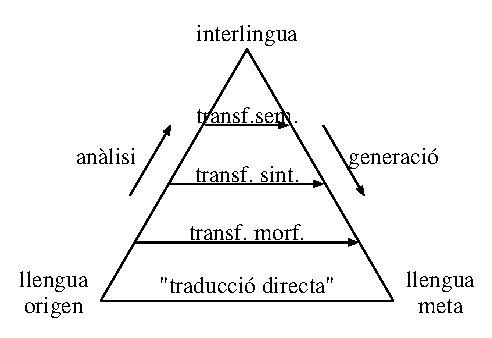
\includegraphics{triangle}
\end{center}
\caption{Com més profunda i complexa és l'anàlisi del text origen, més
  senzilla és (menys esforç comporta) la transferència a la
  representació corresponent de la llengua meta i més complexa la
  generació.  L'anàlisi del text origen és tan profunda en els
  sistemes d'interlingua clàssics que no és necessària la
  transferència.}
\label{fg:triangle}
\end{figure}

Les interlingües poden ser de molts tipus. Els sistemes clàssics usen
representacions estructurals més o menys complexes per a representar
les relacions semàntiques entre els elements de la frase. 
% (de l'estil de les de la solució a l'exercici~\ref{exer:agradar}).  
Però les interlingües no han de ser necessàriament el resultat d'una
anàlisi profunda: el que han de ser necessàriament és \emph{neutrals};
per exemple, alguns sistemes històrics com DLT
\citep[cap.~17]{hutchins92b} usen com a \emph{interlingua} una llengua
\emph{pivot} ``natural'' com l'esperanto, amb anotacions que resolen
algunes ambigüitats típiques.\footnote{Aquesta aproximació pot ser
  particularment útil quan les llengües entre les quals ha de traduir
  el sistema tenen una gran similitud sintàctica i semàntica, com en
  el cas de les llengües romàniques, amb l'excepció, potser, del
  romanés.}

En l'intent de representar els significats de totes les frases de
totes les llengües, les interlingües clàssiques acabarien per ser
``models del món''. Això fa que, actualment, només s'hagen
desenvolupat sistemes d'interlingua clàssics per a àmbits temàtics
molt concrets.

Un dels avantatges més importants dels sistemes d'interlingua respecte
dels sistemes de transferència és la facilitat amb què es pot afegir
una llengua nova a un sistema de traducció automàtica multilingüe.
Imaginem tres llengües que anomenarem $L_1$, $L_2$ i $L_3$. Un sistema
complet de transferència que traduïra entre aquestes tres llengües en
els dos sentits tindria tres mòduls d'anàlisi (que anomenarem $A_1$,
$A_2$ i $A_3$), tres mòduls de generació (que anomenarem $G_1$, $G_2$
i $G_3$) i sis mòduls de transferència (que anomenarem $T_{12}$,
$T_{13}$, $T_{23}$, $T_{31}$, $T_{32}$ i $T_{21}$).\footnote{En
  general, per a $N$ llengües $L_1, L_2, \ldots, L_N$ hi hauria $N$
  mòduls d'anàlisi, $N$ mòduls de generació i $N(N-1)$ mòduls de
  transferència.} Afegir un quart idioma $L_4$ al sistema comporta:
\begin{itemize}
\item Crear un nou mòdul d'anàlisi ($A_4$).
\item Crear un nou mòdul de generació ($G_4$).
\item Construir 6 nous mòduls de transferència ($T_{14}$, $T_{24}$,
  $T_{34}$, $T_{41}$, $T_{42}$ i $T_{43}$). Notem que per a aquesta
  última fase són necessaris diversos experts bilingües en sistemes de
  transferència.\footnote{En el cas general d'afegir una llengua a un
    conjunt de $N$ llengües, calen $2N$ nous mòduls de transferència.}
\end{itemize}
La figura~\ref{fg:afetran} il·lustra el cost d'afegir $L_4$ al sistema
de transferència;
\begin{figure}
\begin{center}
%TexCad Options
%\grade{\off}
%\emlines{\off}
%\beziermacro{\on}
%\reduce{\on}
%\snapping{\off}
%\quality{2.00}
%\graddiff{0.01}
%\snapasp{1}
%\zoom{1.00}
{\scriptsize 
\unitlength 0.80mm
\linethickness{0.4pt}
\begin{picture}(155.00,100.00)
\put(110.00,10.00){\makebox(0,0)[cc]{$L_3$}}
\put(110.00,25.00){\makebox(0,0)[cc]{$RA_3$}}
\put(110.00,85.00){\makebox(0,0)[cc]{$RA_1$}}
\put(110.00,100.00){\makebox(0,0)[cc]{$L_1$}}
\put(80.00,55.00){\makebox(0,0)[cc]{$RA_2$}}
\put(65.00,55.00){\makebox(0,0)[cc]{$L_2$}}
\put(140.00,55.00){\makebox(0,0)[cc]{$RA_4$}}
\put(155.00,55.00){\makebox(0,0)[cc]{$L_4$}}
%\vector(152.00,57.00)(143.00,57.00)
\put(143.00,57.00){\vector(-1,0){0.2}}
\put(152.00,57.00){\line(-1,0){9.00}}
%\end
%\vector(143.00,53.00)(152.00,53.00)
\put(152.00,53.00){\vector(1,0){0.2}}
\put(143.00,53.00){\line(1,0){9.00}}
%\end
%\vector(108.00,97.00)(108.00,88.00)
\put(108.00,88.00){\vector(0,-1){0.2}}
\put(108.00,97.00){\line(0,-1){9.00}}
%\end
%\vector(112.00,88.00)(112.00,97.00)
\put(112.00,97.00){\vector(0,1){0.2}}
\put(112.00,88.00){\line(0,1){9.00}}
%\end
%\vector(68.00,53.00)(77.00,53.00)
\put(77.00,53.00){\vector(1,0){0.2}}
\put(68.00,53.00){\line(1,0){9.00}}
%\end
%\vector(77.00,57.00)(68.00,57.00)
\put(68.00,57.00){\vector(-1,0){0.2}}
\put(77.00,57.00){\line(-1,0){9.00}}
%\end
%\vector(108.00,22.00)(108.00,13.00)
\put(108.00,13.00){\vector(0,-1){0.2}}
\put(108.00,22.00){\line(0,-1){9.00}}
%\end
%\vector(112.00,13.00)(112.00,22.00)
\put(112.00,22.00){\vector(0,1){0.2}}
\put(112.00,13.00){\line(0,1){9.00}}
%\end
\put(104.00,93.00){\makebox(0,0)[cc]{$A_1$}}
\put(116.00,93.00){\makebox(0,0)[cc]{$G_1$}}
\put(72.00,61.00){\makebox(0,0)[cc]{$G_2$}}
\put(72.00,49.00){\makebox(0,0)[cc]{$A_2$}}
\put(148.00,49.00){\makebox(0,0)[cc]{$G_4$}}
\put(148.00,61.00){\makebox(0,0)[cc]{$A_4$}}
\put(116.00,17.00){\makebox(0,0)[cc]{$A_3$}}
\put(104.00,17.00){\makebox(0,0)[cc]{$G_3$}}
\put(108.00,82.00){\vector(0,-1){47.00}}
\put(83.00,53.00){\vector(1,0){47.00}}
\put(137.00,57.00){\vector(-1,0){47.00}}
\put(112.00,28.00){\vector(0,1){47.00}}
\put(137.00,57.00){\vector(-1,1){21.00}}
\put(108.00,81.67){\vector(-1,-1){21.00}}
\put(83.00,53.00){\vector(1,-1){21.00}}
\put(112.00,28.00){\vector(1,1){21.00}}
\put(83.00,53.00){\vector(1,1){21.00}}
\put(112.00,28.00){\vector(-1,1){22.00}}
\put(137.00,57.00){\vector(-1,-1){21.00}}
\put(108.00,82.00){\vector(1,-1){22.00}}
\put(130.00,70.00){\makebox(0,0)[cc]{$T_{41}$}}
\put(125.00,35.00){\makebox(0,0)[cc]{$T_{34}$}}
\put(90.00,40.00){\makebox(0,0)[cc]{$T_{23}$}}
\put(95.00,75.00){\makebox(0,0)[cc]{$T_{12}$}}
\put(100.00,65.00){\makebox(0,0)[cc]{$T_{21}$}}
\put(120.33,45.33){\makebox(0,0)[cc]{$T_{43}$}}
\put(120.00,65.00){\makebox(0,0)[cc]{$T_{14}$}}
\put(100.00,45.00){\makebox(0,0)[cc]{$T_{32}$}}
\put(100.00,50.00){\makebox(0,0)[cc]{$T_{24}$}}
\put(120.00,60.00){\makebox(0,0)[cc]{$T_{42}$}}
\put(116.00,45.33){\makebox(0,0)[cc]{$T_{31}$}}
\put(105.00,65.00){\makebox(0,0)[cc]{$T_{13}$}}
\put(45.00,10.00){\makebox(0,0)[cc]{$L_3$}}
\put(45.00,25.00){\makebox(0,0)[cc]{$RA_3$}}
\put(45.00,85.00){\makebox(0,0)[cc]{$RA_1$}}
\put(45.00,100.00){\makebox(0,0)[cc]{$L_1$}}
\put(15.00,55.00){\makebox(0,0)[cc]{$RA_2$}}
\put(0.00,55.00){\makebox(0,0)[cc]{$L_2$}}
%\vector(43.00,97.00)(43.00,88.00)
\put(43.00,88.00){\vector(0,-1){0.2}}
\put(43.00,97.00){\line(0,-1){9.00}}
%\end
%\vector(47.00,88.00)(47.00,97.00)
\put(47.00,97.00){\vector(0,1){0.2}}
\put(47.00,88.00){\line(0,1){9.00}}
%\end
%\vector(3.00,53.00)(12.00,53.00)
\put(12.00,53.00){\vector(1,0){0.2}}
\put(3.00,53.00){\line(1,0){9.00}}
%\end
%\vector(12.00,57.00)(3.00,57.00)
\put(3.00,57.00){\vector(-1,0){0.2}}
\put(12.00,57.00){\line(-1,0){9.00}}
%\end
%\vector(43.00,22.00)(43.00,13.00)
\put(43.00,13.00){\vector(0,-1){0.2}}
\put(43.00,22.00){\line(0,-1){9.00}}
%\end
%\vector(47.00,13.00)(47.00,22.00)
\put(47.00,22.00){\vector(0,1){0.2}}
\put(47.00,13.00){\line(0,1){9.00}}
%\end
\put(39.00,93.00){\makebox(0,0)[cc]{$A_1$}}
\put(51.00,93.00){\makebox(0,0)[cc]{$G_1$}}
\put(7.00,61.00){\makebox(0,0)[cc]{$G_2$}}
\put(7.00,49.00){\makebox(0,0)[cc]{$A_2$}}
\put(51.00,17.00){\makebox(0,0)[cc]{$A_3$}}
\put(39.00,17.00){\makebox(0,0)[cc]{$G_3$}}
\put(43.00,82.00){\vector(0,-1){47.00}}
\put(47.00,28.00){\vector(0,1){47.00}}
\put(43.00,81.67){\vector(-1,-1){21.00}}
\put(18.00,53.00){\vector(1,-1){21.00}}
\put(18.00,53.00){\vector(1,1){21.00}}
\put(47.00,28.00){\vector(-1,1){22.00}}
\put(25.00,40.00){\makebox(0,0)[cc]{$T_{23}$}}
\put(30.00,75.00){\makebox(0,0)[cc]{$T_{12}$}}
\put(35.00,65.00){\makebox(0,0)[cc]{$T_{21}$}}
\put(35.00,45.00){\makebox(0,0)[cc]{$T_{32}$}}
\put(51.00,45.33){\makebox(0,0)[cc]{$T_{31}$}}
\put(40.00,65.00){\makebox(0,0)[cc]{$T_{13}$}}
\end{picture}
}
\end{center}
\caption{Cost d'afegir una quarta llengua $L_4$ a un sistema de
  transferència. Les entitats $RA_1$ a $RA_4$ són les representacions
  abstractes (tant RALO com RALM) que usen els mòduls de
  transferència.}
\label{fg:afetran}
\end{figure}
En canvi, en un sistema d'interlingua no hi ha mòduls de
transferència; un sistema trilingüe basat en una interlingua tindria
només sis mòduls: tres d'anàlisi ($A'_1$, $A'_2$ i $A'_3$) i tres de
generació ($G'_1$, $G'_2$ i $G'_3$). Queda clar que els mòduls
d'anàlisi i de generació en aquests sistemes són més complexos que en
el cas de transferència (ja que han de fer transformacions cap a
estructures lingüísticament neutrals), però també és clar l'avantatge
del sistema d'interlingua a l'hora d'afegir-hi la llengua $L_4$: només
cal dissenyar dos mòduls nous, $A'_4$ i $G'_4$, i per a dissenyar-los
només necessitem una persona que conega bé la llengua $L_4$ i la
interlingua $I$ que usa el sistema. La figura~\ref{fg:afeinte}
il·lustra el cost d'afegir $L_4$ al sistema.
\begin{figure}
\begin{center}
%TexCad Options
%\grade{\off}
%\emlines{\off}
%\beziermacro{\on}
%\reduce{\on}
%\snapping{\off}
%\quality{2.00}
%\graddiff{0.01}
%\snapasp{1}
%\zoom{1.00}
\unitlength 1.00mm
\linethickness{0.4pt}
\begin{picture}(100.00,50.00)
\put(60.00,30.00){\makebox(0,0)[cc]{$L_2$}}
\put(80.00,10.00){\makebox(0,0)[cc]{$L_3$}}
\put(80.00,50.00){\makebox(0,0)[cc]{$L_1$}}
\put(100.00,30.00){\makebox(0,0)[cc]{$L_4$}}
\put(80.00,30.00){\makebox(0,0)[cc]{$I$}}
%\vector(78.00,33.00)(78.00,45.00)
\put(78.00,45.00){\vector(0,1){0.2}}
\put(78.00,33.00){\line(0,1){12.00}}
%\end
%\vector(82.00,47.00)(82.00,35.00)
\put(82.00,35.00){\vector(0,-1){0.2}}
\put(82.00,47.00){\line(0,-1){12.00}}
%\end
%\vector(83.00,32.00)(95.00,32.00)
\put(95.00,32.00){\vector(1,0){0.2}}
\put(83.00,32.00){\line(1,0){12.00}}
%\end
%\vector(97.00,28.00)(85.00,28.00)
\put(85.00,28.00){\vector(-1,0){0.2}}
\put(97.00,28.00){\line(-1,0){12.00}}
%\end
%\vector(82.00,27.00)(82.00,15.00)
\put(82.00,15.00){\vector(0,-1){0.2}}
\put(82.00,27.00){\line(0,-1){12.00}}
%\end
%\vector(78.00,13.00)(78.00,25.00)
\put(78.00,25.00){\vector(0,1){0.2}}
\put(78.00,13.00){\line(0,1){12.00}}
%\end
%\vector(77.00,28.00)(65.00,28.00)
\put(65.00,28.00){\vector(-1,0){0.2}}
\put(77.00,28.00){\line(-1,0){12.00}}
%\end
%\vector(63.00,32.00)(75.00,32.00)
\put(75.00,32.00){\vector(1,0){0.2}}
\put(63.00,32.00){\line(1,0){12.00}}
%\end
\put(70.00,36.00){\makebox(0,0)[cc]{$A'_2$}}
\put(90.00,36.00){\makebox(0,0)[cc]{$G'_4$}}
\put(90.00,24.00){\makebox(0,0)[cc]{$A'_4$}}
\put(70.00,24.00){\makebox(0,0)[cc]{$G'_2$}}
\put(74.00,40.00){\makebox(0,0)[cc]{$G'_1$}}
\put(74.00,20.00){\makebox(0,0)[cc]{$A'_3$}}
\put(86.00,20.00){\makebox(0,0)[cc]{$G'_3$}}
\put(86.00,40.00){\makebox(0,0)[cc]{$A'_1$}}
\put(10.00,30.00){\makebox(0,0)[cc]{$L_2$}}
\put(30.00,10.00){\makebox(0,0)[cc]{$L_3$}}
\put(30.00,50.00){\makebox(0,0)[cc]{$L_1$}}
\put(30.00,30.00){\makebox(0,0)[cc]{$I$}}
%\vector(28.00,33.00)(28.00,45.00)
\put(28.00,45.00){\vector(0,1){0.2}}
\put(28.00,33.00){\line(0,1){12.00}}
%\end
%\vector(32.00,47.00)(32.00,35.00)
\put(32.00,35.00){\vector(0,-1){0.2}}
\put(32.00,47.00){\line(0,-1){12.00}}
%\end
%\vector(32.00,27.00)(32.00,15.00)
\put(32.00,15.00){\vector(0,-1){0.2}}
\put(32.00,27.00){\line(0,-1){12.00}}
%\end
%\vector(28.00,13.00)(28.00,25.00)
\put(28.00,25.00){\vector(0,1){0.2}}
\put(28.00,13.00){\line(0,1){12.00}}
%\end
%\vector(27.00,28.00)(15.00,28.00)
\put(15.00,28.00){\vector(-1,0){0.2}}
\put(27.00,28.00){\line(-1,0){12.00}}
%\end
%\vector(13.00,32.00)(25.00,32.00)
\put(25.00,32.00){\vector(1,0){0.2}}
\put(13.00,32.00){\line(1,0){12.00}}
%\end
\put(20.00,36.00){\makebox(0,0)[cc]{$A'_2$}}
\put(20.00,24.00){\makebox(0,0)[cc]{$G'_2$}}
\put(24.00,40.00){\makebox(0,0)[cc]{$G'_1$}}
\put(24.00,20.00){\makebox(0,0)[cc]{$A'_3$}}
\put(36.00,20.00){\makebox(0,0)[cc]{$G'_3$}}
\put(36.00,40.00){\makebox(0,0)[cc]{$A'_1$}}
\end{picture}
\end{center}
\caption{Cost d'afegir una quarta llengua $L_4$ a un sistema
  d'interlingua.}
\label{fg:afeinte}
\end{figure} 

\section{Sistemes de traducció automàtica basats en corpus}
\label{ss:induc}
Totes les tècniques de traducció automàtica descrites fins ara són de
naturalesa \emph{deductiva}, és a dir, estan basades en teories i
coneixements lingüístics sobre la traducció. Però recentment (sobretot
en els primers anys del tercer mil·lenni) s'està produint un
creixement espectacular de tècniques \emph{inductives} de traducció
automàtica, en les quals el sistema \emph{aprén} automàticament a
traduir entre dues llengües a partir d'un corpus paral·lel
suficientment gran d'oracions en LO acompanyades de la seua traducció
a la LM (vegeu l'apartat~\ref{ss:bitextos}). Aquestes aproximacions
inductives també reben el nom de \emph{traducció automàtica basada en
  corpus}.

\subsection{Sistemes de traducció automàtica estadística}
\label{ss:tae}
La principal tècnica de traducció automàtica basada en corpus es la
\emph{traducció automàtica estadística} (en anglés \emph{statistical
  machine translation}; SMT), la qual va ser inventada cap a finals
dels huitanta per un grup d'investigadors d'IBM \citep{brown90j}; els
sistemes actuals són una evolució d'aquests.

A l'hora de traduir hi ha una diferència fonamental entre els sistemes
basats en regles o coneixement i els sistemes estadístics: mentres que
els sistemes basat en regles produeixen únicament una traducció, els
sistemes estadístics generen una gran quantitat d'\emph{hipòtesis de
  traducció} (idealment totes les possibles) i utilitzen models
estadístics per \emph{puntuar} les hipòtesis generades i escollir la
millor de totes. Els principals models estadístics que s'usen per
puntuar les hipòtesis de traducció són el \emph{model de traducció} i
el \emph{model de llengua}, els quals s'expliquen més avall. La
combinació d'aquests models fa que la hipòtesi de traducció que rep
la puntuació \emph{global} més alta no siga necessàriament la hipòtesi
de traducció millor segons cada model per separat.

\begin{figure}
\centering
\begin{tabular}{p{6cm}|p{6cm}}
  \multicolumn{1}{c|}{\textbf{Anglés}} & \multicolumn{1}{c}{\textbf{Espanyol}}\\
  \hline
  It has been exciting in many ways . &
  Ha sido un trabajo apasionante en varios sentidos . \\
  \hline
  As the shadow rapporteurs know , this has been my first report
  during my time in Parliament and it has been a good learning
  experience . &
  Como bien saben los ponentes alternativos , éste ha sido el primer
  informe en el que he trabajado durante mi mandato parlamentario , y
  me ha venido muy bien como experiencia formativa . \\
  \hline
  It has also been very challenging to work on three reports and
  therefore also with other rapporteurs . &
  También ha sido un gran desafío trabajar en tres informes , y por lo
  tanto con otros ponentes . \\
  \hline
  It has been exciting . &
  Ha sido emocionante . \\
  \hline
\end{tabular}
\caption{Oracions paral·leles anglés-espanyol extretes del corpus
  paral·lel Europarl (\texttt{http://www.statmt.org/europarl/}) amb
  les actes del Parlament Europeu de període 1996--2011.}
\label{fg:alinora}
\end{figure}


\begin{figure}
\centering
\includegraphics[scale=0.5]{alin-paraules}
\caption{Alineament entre les paraules de l'oració en anglés
  \emph{The white bird decided to fly.} and les paraules de l'oració en
català \emph{El pardal blanc va decidir volar.}}
\label{fg:alinpar}
\end{figure}

El \textbf{model de traducció} s'aprén a partir d'un corpus paral·lel
amb les oracions ja alineades com el que es mostra en la figura
\ref{fg:alinora}. Primerament, s'han d'obtenir els \emph{alineaments
  entre els mots} (vegeu-ne un exemple en la figura \ref{fg:alinpar})
per a després estimar el model de traducció a partir d'aquests
alineaments.

\begin{figure}[tb]
  \centering %
  \subfigure[\label{fg:pasosalin1}Inicialització: Tots els alineament
  són igualment probables.]{\includegraphics[scale=0.5]{ibm1/ibm2}} 

  \subfigure[\label{fg:pasosalin2}Primera iteració: El alineament
  entre \emph{yn} i \emph{gur} guanya
  força.]{\includegraphics[scale=0.5]{ibm1/ibm3}}

  \subfigure[\label{fg:pasosalin3}Segona iteració: El alineament entre
  \emph{pifo} i \emph{ubhfo} guanya
  força.]{\includegraphics[scale=0.5]{ibm1/ibm4}}

  \subfigure[\label{fg:pasosalin4}Tercera i última iteració:
  L'estructura d'alineament que estava ``oculta'' queda al
  descobert.]{\includegraphics[scale=0.5]{ibm1/ibm5}}
  \caption{Exemple que il·lustra el procés iteratiu que permet obtenir
    l'alineament entre les paraules de les oracions d'un corpus
    paral·lel. En aquest exemple el corpus consta de tres oracions
    paral·leles en dos llengües inventades. Aquestes oracions
    paral·leles són: \emph{yn pifo}--\emph{gur ubhfo}, \emph{yn pifo
      oynapi}--\emph{gur juvga ubhfo} i \emph{yn sybe}--\emph{gur
      subjre}. El gruix de les línies que connecten les paraules
    representa la probabilitat de l'alineament.}
\label{fg:pasosalin}
\end{figure}

Tot i que sembla una tasca difícil per a un ordinador, els alineaments
entre els mots es poden obtenir automàticament sense usar cap
coneixement sobre les llengües dels textos a alinear mitjançat un
procés iteratiu. La figura \ref{fg:pasosalin} il·lustra aquest procés
amb un corpus menut de tres oracions paral·leles; si us fixeu, sense
tenir cap coneixement de les llengües (perquè han estat inventades)
les persones també som capaces d'obtenir aquests alineaments. El
procés comença assumint que, per a cada oració paral·lela, tots els
mots de l'oració en LM poden ser traducció de cadascun dels mots de
l'oració en LO, i per tant, els assigna la mateixa probabilitat.  En
cada iteració el programa alineador visita totes les oracions
paral·leles del corpus i va refinant aquestes probabilitats fins que
l'estructura d'alineament queda definida. Aquest refinament es
produeix perquè en cada iteració les probabilitats de la iteració
anterior s'usen per acumular evidència en tot el corpus sobre la
probabilitat de les correspondències entre mots i, a més, perquè els
mots que són traducció mútua solen aparéixer junts en les mateixes
oracions paral·leles, la qual cosa no succeeix si dos mots no són
traducció un de l'altre.

Una vegada obtinguts els alineaments entre els mots, podem aprendre
models probabilístics que indiquen, per exemple, la probabilitat que
la traducció d'un determinat mot en una llengua siga la traducció d'un
determinat mot en l'altra (un model de traducció de paraules o
diccionari bilingüe probabilístic), o la probabilitat que la traducció
d'una seqüència (segment) de mots en una llengua siga la traducció
d'una seqüència (segment) de mots en l'altra (un model de traducció de
segments). Aquest últim model l'usen els sistemes de traducció
automàtica estadística basats en segments bilingües (en anglés
\emph{phrase-based statistical machine translation}; \cite{koehnbook}),
els quals són els més usats en l'actualitat.

Però per produir bones traduccions no podem usar el model de traducció
únicament perquè les traduccions serien poc naturals, gramaticals i
fluides. El motiu és que el model de traducció no té en compte l'ordre
en què apareixen els segments traduïts en la LM, ni el context en què
apareixen els segments en LO a l'hora de puntuar les seues possibles
traduccions. Aquestes deficiències es mitiguen parcialment amb l'ús
d'un model de la LM.

Un \textbf{model de llengua} és un model probabilístic que serveix per
a mesurar la versemblança d'una oració o text en LM; és a dir, la seua
fluïdesa o gramaticalitat.\footnote{S'assumeix que el model de llengua
  s'aprén de textos naturals i gramaticalment correctes en LM.}
Aquests models s'aprenen de forma automàtica a partir d'un corpus de
text en LM i es basen en comptar la freqüència de segments de longitud
fixa, normalment segments de fins a cinc paraules, per evitar assignar
una versemblança nul·la a oracions que, tot i que són correctes, no
apareixen en els corpus d'entrenament.\footnote{Per evitar assignar
  versemblances nul·les a una oració, a més d'utilitzar segments de
  poques paraules, aquests models també usen tècniques de suavitzat
  (en anglés \emph{smoothing}) de les probabilitat.} El model de
llengua té en compte l'ordre de les paraules i per tant assigna una
versemblança major a l'oració \emph{M'agrada menjar pernil del bo} que
a l'oració \emph{del bo menjar pernil M'agrada}, tot i que contenen
els mateixos segments de text (\emph{del bo}, \emph{menjar pernil} i
\emph{M'agrada}). A més té en compte, tot i que indirectament, el
context en què apareixen les paraules en LM, de manera que assigna
una versemblança major a l'oració en espanyol (LM) \emph{No piensa con
  la cabeza} que a l'oració \emph{No piensa con el cabo}, on els
segments \emph{la cabeza} i \emph{el cabo} són dues possibles
traduccions del segment en català \emph{el cap} que apareix en
l'oració en LO \emph{No pensa amb el cap}.

\begin{persabermes}{sistemes de traducció automàtica estadística}
  A més dels models de traducció i de la LM els sistemes de traducció
  automàtica estadística basats en segments bilingües combinen altres
  models per a establir la puntuació global d'una hipòtesi de
  traducció. A continuació es descriuen molt breument aquests models i
  per a què s'usen:
  \begin{description}
  \item[Model de reordenament lèxic:] La seua funció és modelar
    diferents operacions de reordenament que es poden fer a l'hora de
    disposar les traduccions dels segments en LO. Les probabilitats
    d'aquestes operacions depenen dels segments concrets que s'estan
    reordenant i són tres: traducció monòtona (quan no hi ha
    reordenament), reordenament (quan la posició de la traducció del
    segment en qüestió i la de l'anterior s'intercanvien) i traducció
    discontinua (qual la traducció del segment es mou a una altra
    posició en l'oració en LM; es a dir, quan no és cap de les altres
    dues operacions).
  \item[Ponderació lèxica:] Els segments usats per traduir poden ser
    molt llargs (normalment fins a 7 paraules), la qual cosa fa molt
    difícil estimar bé la seua probabilitat de traducció perquè els
    segments llargs solen aparéixer poques vegades en els corpus
    d'entrenament; això fa necessari l'ús d'un altre model per estimar
    la qualitat dels segments bilingües. Aquest model usa les
    probabilitats de traducció entre els mots (un diccionari bilingüe
    probabilístic) per obtenir un indicador de la qualitat d'els
    segments bilingües. Per exemple, la qualitat del segment bilingüe
    (\emph{la comissió de balanços de finançament}, \emph{the funding
      balance comission}), on l'alineament entre els mots és
    \emph{la}--\emph{the}, \emph{comissió}--\emph{comission},
    \emph{balanços}--\emph{balance} i
    \emph{finançament}--\emph{funding}, depén de les probabilitats de
    traducció dels mots que han estat alineats.
  \item[Nombre total de paraules de l'oració:] Quan es puntuen les
    hipòtesis de traducció es multipliquen moltes probabilitats, és a
    dir valors entre 0 i 1, de manera que com més llarga siga una
    traducció més probabilitats es multipliquen i més fàcil és arribar
    a tenir una puntuació molt prop de zero. Això fa que els sistemes
    preferisquen les traduccions curtes. Per a evitar això
    s'introdueix un model que compta el nombre de paraules en la
    hipòtesi de traducció i que fa que tinga relació amb el nombre de
    paraules de l'oració origen.
  \item[Nombre de segments:] Aquest model és similar a l'anterior, però
    comptant el nombre de segments bilingües que s'han usat per a
    produir una hipòtesi de traducció. Com més llargs siguen els
    segments, menys segments s'usaran i més context tindran; i a
    l'inrevés, com més curts siguen els segments més segments faran
    falta per produir la hipòtesi de traducció.
  \end{description}

  Tots aquests models (i els anteriors) es combinen per a obtenir una
  puntuació global per a cada hipòtesi de traducció i poder escollir
  així la millor. Aquesta combinació es fa assignant un pes
  (importància) a cada model que s'obté mitjançat un procés automàtic
  (\emph{tuning}) que intenta maximitzar la \emph{qualitat} de les
  traduccions proporcionades pel sistema en traduir un corpus de
  \emph{desenvolupament}.  

  Consulteu el llibre de \citet{koehnbook} per saber més sobre els
  models que s'usen per a traduir, el procés de \emph{tuning} i les
  mesures automàtiques de la qualitat que usen.
\end{persabermes}


\begin{persabermes}{sistemes basats en corpus}
  Hi ha hagut altres aproximacions inductives a la traducció
  automàtica, com ara els sistemes de \emph{traducció automàtica
    basada en exemples}, tot i que a hores d'ara ja no s'usen.  La
  \emph{traducció automàtica basada en exemples} intenta construir
  \emph{plantilles} de traducció a partir dels exemples observats en
  el corpus d'oracions paral·leles i \emph{generalitzar-les} perquè
  servisquen en noves situacions. Per exemple, si sabem que el
  substantiu anglés \emph{ski} es tradueix per \emph{esquí} i que la
  locució substantiva \emph{ski station} es tradueix per \emph{estació
    d'esquí} podem generalitzar aquesta última locució substituint
  \emph{ski} per qualsevol altres substantiu $N$, de manera que la
  traducció de ``$N$ \emph{station}'' és ``estació de $N$''; així, si
  la traducció de \emph{train} és \emph{tren}, la traducció de
  \emph{train station} és \emph{estació de tren}, etc. (exemple pres
  de \citealt{carl01j}). Fixeu-vos que la traducció automàtica basada
  en exemples pot necessitar que la mostra de frases i traduccions
  estiga, a més, anotada lingüísticament (en l'exemple, indicant quins
  mots o estructures funcionen com un nom).
\end{persabermes}


\section{Qüestions i exercicis}
Els exercicis marcats amb (*) són més difícils.

\begin{enumerate}
\item Els sistemes de traducció mot per mot poden cometre, per
  exemple, errors en la concordança de gènere o de nombre.  Elegiu
  dues llengües $L_1$ i $L_2$ i poseu almenys dos exemples de
  traduccions mot per mot de $L_1$ a $L_2$ amb problemes de
  concordança.

\item (*) \label{ex:cascat} CasCat és un sistema de traducció
  automàtica de l'espanyol al català que usa regles que reordenen
  seqüències de formes lèxiques segons les categories lèxiques. Les
  regles s'apliquen de la manera usual: d'esquerra a dreta, reordenant
  la seqüència més llarga possible, i sense que se solapen les àrees
  reordenades.  Heus ací algunes frases espanyoles amb {\em cuyo}, les
  traduccions produïdes per CasCat, i, on la traducció és incorrecta,
  una alternativa acceptable.
  \begin{enumerate}
  \item \emph{La chica cuyos compañeros murieron es china} \newline
    {\em La noia els companys de la qual van morir és xinesa}
  \item \emph{La chica cuyos compañeros de clase murieron es china}
    \newline \emph{La noia els companys de classe de la qual van morir
      és xinesa}
  \item \emph{La chica cuyos compañeros mayores murieron es china}
    \newline \emph{La noia els companys grans de la qual van morir és
      xinesa}
  \item \emph{La chica cuyos compañeros de clase de francés murieron
      es china} \newline \emph{*La noia els companys de classe de la
      qual de francès van morir és xinesa} \newline (\emph{La noia els
      companys de classe de francès de la qual van morir és xinesa})
  \item \emph{La chica cuyos compañeros mayores de classe murieron es
      china} \newline \emph{*La noia els companys grans de la qual de
      classe van morir és xinesa} \newline (\emph{La noia els companys
      grans de classe de la qual van morir és xinesa})
  \item \emph{La chica cuyos compañeros mayores de clase de francés
      murieron es china} \newline \emph{*La noia els companys grans de
      la qual de classe de francès van morir és xinesa} \newline
    (\emph{La noia els companys grans de classe de francès de la qual
      van morir és xinesa})
  \end{enumerate}
  Les traduccions inacceptables estan marcades amb un asterisc.
  Proposeu un conjunt de regles de reordenament que expliquen el
  conjunt de traduccions observat. En quins casos es ``trenquen''
  sintagmes?

\item La multinacional WorldTrans ha decidit ampliar el seu sistema de
  traducció automàtica multilingüe LetTrans (que tradueix
  correspondència comercial entre qualssevol dues llengües d'un grup
  de quinze) i afegir-hi la capacitat de traduir del suahili a les
  quinze llengües i de les quinze llengües cap al suahili. En una
  oferta de treball, WorldTrans demana experts en suahili però no
  demana cap expert en traducció entre suahili i cap de les quinze
  llengües. Quina classe de sistema de traducció automàtica és
  LetTrans?  Justifiqueu la resposta.

\item (*) Imagineu que teniu un sistema de traducció automàtica que
  treballa amb dues llengües, diguem-ne $A$ i $B$, en els dos sentits
  de traducció: $A{\rightarrow}B$ i $B{\rightarrow}A$, que traduïm un
  text origen $T$ en llengua $A$ a la llengua $B$ mitjançant aquest
  traductor automàtic, generant un text $T'$, i que després usem
  aquest mateix sistema per a traduir $T'$ de nou a la llengua $A$;
  anomenarem $T''$ el nou text en llengua $A$.
  \begin{equation}
    T \stackrel{\scriptsize A\rightarrow
      B}{\longrightarrow}T'\stackrel{\scriptsize B\rightarrow
      A}{\longrightarrow} T''
  \end{equation}
  El text $T''$ serà previsiblement diferent del text $T$.  Trieu dues
  llengües $A$ i $B$ i indiqueu quins canvis són previsibles,
  classificant-los segons la naturalesa lingüística dels fenòmens que
  han causat els canvis, explicant la raó del resultat si cal amb un
  exemple. Heu d'indicar \emph{tres tipus diferents} de canvi.

\item (*) Imagineu que sou part d'un equip de desenvolupament d'un
  sistema de traducció automàtica de l'anglés al català basat en
  l'estratègia de transferència morfològica avançada
  (apartat~\ref{s3:STMorf}). Els informàtics del projecte us demanen
  consell sobre les regles de reordenament del sistema, ja que, per
  motius tècnics, només poden afegir-n'hi tres.
      
  Indiqueu quines serien les 3 regles que proposaríeu, tenint en
  compte que han de produir, com a mínim, tres oracions ben traduïdes
  en el corpus d'oracions següents (la traducció ideal s'indica entre
  parèntesis, tot i que no sempre podrà ser aconseguida):
  \begin{enumerate}
  \item \emph{A dark autumn night} (\emph{Una nit fosca de
      tardor})
  \item \emph{A high tide} (\emph{Una marea alta}) 
  \item \emph{A magic dark silhouette} (\emph{Una silueta fosca
      màgica})
  \item \emph{An autumn tide} (\emph{Una marea de tardor})
  \item \emph{A dark magic silhouette} (\emph{Una silueta màgica
      fosca})
  \item \emph{A dark autumn high tide} (\emph{Una marea alta de
      tardor fosca})
  \item \emph{A dark night} (\emph{Una nit fosca})
  \end{enumerate}
    
  Deixeu de banda la concordança i centreu-vos només en els
  reordenaments. Assenyaleu quina seria la traducció del sistema per a
  totes les oracions anteriors usant el conjunt de regles que heu
  proposat.

\item Quina és l'operació inversa de l'anàlisi morfològica?
  \begin{enumerate}
  \item L'obtenció de la forma lèxica d'un mot a partir de la forma
    superficial.
  \item La generació morfològica.
  \item La transferència morfològica.
  \end{enumerate}

\item La traducció automàtica per transferència és sempre...
  \begin{enumerate}
  \item ... morfològica.
  \item ... directa.
  \item ... indirecta.
  \end{enumerate}

\item (*) Dues traduccions possibles del mot català \emph{cap} a
  l'espanyol són \emph{cabe} o \emph{cabeza}. Com podria fer l'elecció
  adequada un sistema de traducció automàtica?
  \begin{enumerate}
  \item Posant-hi la traducció més probable, basada en les freqüències
    d'ús dels mots.
  \item Usant informació morfosintàctica, ja que en la posició
    concreta de la frase podria anar només un verb o un substantiu.
  \item No podria, perquè les dues traduccions són sempre possibles en
    qualsevol frase.
  \end{enumerate}

\item Quines de les següents representacions intermèdies son més
  costoses d'obtenir a partir de les frases?
  \begin{enumerate}
  \item Els arbres d'anàlisi sintàctica corresponents.
  \item Les seqüències de categories morfològiques corresponents.
  \item Les estructures semàntiques superficials corresponents.
  \end{enumerate}

%\item Només una d'aquestes operacions és esperable en una situació
%  normal de traducció automàtica. Quina?
%  \begin{enumerate}
%  \item La postedició en un sistema de traducció automàtica usat per a
%    l'assimilació.
%  \item Una fase complexa de transferència en un sistema
%    d'interlingua.
%  \item La preedició en un sistema de traducció automàtica usat per a
%    la disseminació.
%  \end{enumerate}
      
\item L'anàlisi morfològica pren una oració i...
  \begin{enumerate}
  \item ... produeix un arbre d'anàlisi.
  \item ... produeix, per a cada mot, totes les formes superficials
    corresponents.
  \item ... produeix, per a cada mot, totes les tripletes
    lema--categoria--informació morfològica possibles.
  \end{enumerate}

\item Quines són les fases bàsiques d'un sistema de traducció
  automàtica indirecta?
  \begin{enumerate}
  \item Anàlisi, generació i traducció.
  \item Anàlisi, transferència i generació.
  \item Anàlisi i transferència.
  \end{enumerate}

\item Quin dels següents tipus de sistema de traducció automàtica
  faciliten més l'addició d'una nova llengua?
  \begin{enumerate}
  \item Els sistemes de transferència morfològica avançada.
  \item Els sistemes de transferència semàntica superficial.
  \item Els sistemes d'\emph{interlingua}.
  \end{enumerate}

\item Quin dels següents tipus de sistema de traducció automàtica
  tenen la fase de transferència més senzilla possible?
  \begin{enumerate}
  \item Els sistemes de transferència morfològica avançada.
  \item Els sistemes de transferència semàntica superficial.
  \item Els sistemes d'\emph{interlingua}.
  \end{enumerate}

\item Primerament, elegiu un idioma meta (francés, anglés o alemany) i
  un idioma origen (català o espanyol). Després, per als idiomes
  elegits, doneu un exemple de traducció mot a mot inacceptable en
  \emph{tres} d'aquests cinc casos:
  \begin{enumerate}
  \item homografia mal resolta d'un mot
  \item polisèmia mal resolta d'un mot
  \item problemes de concordança
  \item ambigüitat estructural mal resolta
  \item problemes amb l'ordre dels mots
  \end{enumerate}
      
\item \emph{Interlingua}, a més de ser el nom de la representació
  intermèdia dels sistemes indirectes sense transferència, és el d'una
  llengua artificial bàsicament d'arrel llatina, amb una flexió
  simplificada, i amb un vocabulari dissenyat per a ser comprensible a
  molts europeus.  Una característica important d'interlingua és que
  els determinants (\emph{un}, \emph{le}, \emph{alcun}, \emph{iste},
  \emph{mi}, \emph{tu}, etc.) i els adjectius són invariables. Els
  plurals dels noms es fan amb \emph{-s} o \emph{-es}.  Imagineu que
  tenim un sistema de transferència morfològica avançada que tradueix
  d'interlingua al català (o a l'espanyol) usant aquestes quatre
  regles:
  \begin{itemize}
  \item[$R_1$] detecta \textbf{det}--\textbf{n} i escriu
    \textsf{trad}(\textbf{det})--\textsf{trad}(\textbf{n}), fent
    concordar \textsf{trad}(\textbf{det}) en gènere i en nombre amb
    \textsf{trad}(\textbf{n})
  \item[$R_2$] detecta \textbf{det}--\textbf{n}--\textbf{adj} i escriu
    \textsf{trad}(\textbf{det})--\textsf{trad}(\textbf{n})-\textsf{trad}(\textbf{adj}),
    fent concordar \textsf{trad}(\textbf{det}) i
    \textsf{trad}(\textbf{adj})en gènere i en nombre amb
    \textsf{trad}(\textbf{n})
  \item[$R_3$] detecta \textbf{n}--\textbf{adj} i escriu
    \textsf{trad}(\textbf{n})--\textsf{trad}(\textbf{adj}), fent
    concordar \textsf{trad}(\textbf{adj}) en gènere i en nombre amb
    \textsf{trad}(\textbf{n})
  \item[$R_4$] detecta \textbf{adj}--\textbf{n} i escriu
    \textsf{trad}(\textbf{n})--\textsf{trad}(\textbf{adj}), fent
    concordar \textsf{trad}(\textbf{adj}) en gènere i en nombre amb
    \textsf{trad}(\textbf{n})
  \end{itemize}
  Si no es pot usar informació de concordança, la traducció dels
  determinants i els adjectius es fa en masculí singular.  Indica
  quines traduccions al català (o a l'espanyol) produirà aquest
  sistema per a les frases següents i per què:
  \begin{enumerate}
  \item \emph{Un longe viage}
  \item \emph{Un longe viages}
  \item \emph{Un viages longe}
  \item \emph{Longe viages}
  \item \emph{Un governamento non democratic}
  \item \emph{Un governamentos non democratic}
  \item \emph{Tu melior ideales}
  \item \emph{Un bon solution}
  \end{enumerate}

\item (*) La traducció d'una oració es pot veure com una interpretació
  d'aquesta (és a dir, com l'expressió en la llengua meta del seu
  significat). El \emph{principi de composicionalitat semàntica}
  postula que la interpretació d'una oració es construeix combinant
  les interpretacions dels mots seguint precisament les agrupacions
  successives (constituents) que indica l'arbre d'anàlisi sintàctica
  de l'oració, partint dels mots i anant cap a l'arrel de
  l'arbre. Indiqueu en quin (o quins) tipus de sistema de traducció
  automàtica trobem un disseny que aplica, exactament o
  aproximadament, el principi de composicionalitat. Raoneu breument la
  resposta.
      
\item \label{ex:zkanagg} El programari que porten instal·lat les naus
  de la confederació galàctica inclou un programa que tradueix una de
  les llengües majoritàries del planeta Zkanagg, el tazkannwat, al
  català. El sistema és un sistema de transferència morfològica
  avançada estàndard, que llegeix els textos d'esquerra a dreta, mot a
  mot, busca en l'entrada els patrons de categories lèxiques que conté
  en el seu catàleg, selecciona el més llarg, reordena i concorda els
  mots del patró, els escriu, i continua després de la zona
  reordenada. Algunes traduccions són errònies perquè el sistema no té
  un catàleg massa complet de regles. Fixeu-vos en els exemples i
  digueu quins són els patrons que detecta i quines les regles de
  reordenament associades.
     \begin{example}
     \gll Thlong u knaar uw phlagyw.
          {Va adquirir} el navegant el-OBJ control-OBJ
     \glt TA: El navegant va adquirir el control (correcta).
     \glend
     \end{example}
     \begin{example}
     \gll Thlong u knaar qimratt uw phlagyw.
          {Va adquirir} el navegant estelar el-OBJ control-OBJ
     \glt TA: El navegant estelar va adquirir el control (correcta).
     \glend
     \end{example}
     \begin{example}
     \gll Thlong u knaar na Zkannag uw phlagyw.
          {Va adquirir} el navegant de Zkannag el-OBJ control-OBJ
     \glt TA: El navegant de Zkannag va adquirir el control (correcta).
     \glend
     \end{example}
     \begin{example}
     \gll Thlong u knaar qimratt na Zkannag uw phlagyw.
          {Va adquirir} el navegant estelar de Zkannag el-OBJ control-OBJ
     \glt TA: *El navegant estelar va adquirir de Zkannag el control.
     \glt Correcta: El navegant estelar de Zkannag va adquirir el control.
     \glend
     \end{example}

% \item \label{exer:agradar} Les estructures sintàctiques usades per diverses llengües a
%   l'hora d'expressar el fet que alguna acció agrada a algú són molt
%   diverses. La frase ``m'agrada nadar'' té una estructura sintàctica molt
%   diferent en anglés (\ref{ex:angles}) i en alemany (\ref{ex:alemany}).
% \begin{example}
% \gll Peter likes swimming.
%      Peter s'estima nadant.
% \glt\glend
% \label{ex:angles}
% \end{example}
% \begin{example}
% \gll Peter schwimmt gern.
%      Peter nada {amb gust}.
% \glt\glend
% \label{ex:alemany}
% \end{example}
% Altre exemple el tenim en la frase  ``li diuen Joan'':
% \begin{example}
% \gll He is called Joan.
%      Ell és anomenat Joan.
% \glt\glend
% \label{ex:angles2}
% \end{example}
% \begin{example}
% \gll Er hei{\ss}t Joan.
%      Ell {s'anomena}  Joan.
% \glt\glend
% \label{ex:alemany2}
% \end{example}
% En canvi, les estructures que serveixen per a expressar altres
% conceptes poden ser completament paral·leles. Quines conseqüències té
% això per al disseny d'un sistema de traducció automàtica de
% transferència sintàctica entre llengües amb aquestes característiques?
% Com es podrien evitar els problemes observats?

\item Els mots no són tots igualment freqüents en els textos. De fet,
  si ordenem els mots d'un gran corpus de text real (de qualsevol
  tipus i de qualsevol idioma) pel nombre de vegades que hi apareixen,
  començant pel més freqüent, el nombre d'aparicions es redueix
  dramàticament segons que anem baixant per la llista. Típicament, el
  mot més freqüent pot arribar a constituir el 10\% de tot el text,
  però el segon només cobreix al voltant del 5\%, el tercer al voltant
  del 3\%, etc.; quan arribem al 100é mot més freqüent ja hem de
  parlar del 0,1\% (una vegada cada 1.000 mots), i si arribem a la
  posició 1000, del 0,01\% (una vegada cada 10.000 mots).  En resum,
  la distribució no és gens homogènia: uns pocs mots són els més
  freqüents i la majoria són moltíssim menys freqüents. De fet, és
  típic que la majoria dels mots siguen \emph{hapax legomena}, és a
  dir, mots que han aparegut només una vegada en tot el corpus. Si
  haguéreu de supervisar la construcció dels diccionaris d'un sistema
  de traducció automàtica, per a què us podrien servir aquestes
  constatacions estadístiques?

\item (*) \label{ex:postres} Els sistemes de traducció automàtica
  entre dues llengües amb sintaxi similar no necessiten fer massa
  reordenaments perquè l'ordre dels mots no varia massa d'una llengua
  a altra. A pesar d'això, la traducció mot per mot no és practicable
  perquè el gènere i el nombre gramatical d'alguns substantius varia i
  els adjectius, articles, etc., que l'acompanyen no concordarien
  correctament: cast. {\em una señal muy clara\/} $\rightarrow$
  cat. *{\em una senyal molt clara} (correcte: {\em un senyal molt
    clar\/}); cast. {\em me gusta la leche fría} $\rightarrow$
  ital. *{\em mi piace la latte fredda\/} (correcte: {\em mi piace il
    latte freddo}). Una manera d'identificar zones on s'ha d'establir
  la concordança és detectar seqüències de mots, de manera similar a
  com es fa en els sistemes de transferència morfològica, però sense
  reordenar-les. Per exemple, detectar la seqüència {\bf art}--{\bf
    subst} pot servir per propagar el gènere i el nombre del
  substantiu a l'article. Fixeu-vos en les frases espanyoles següents
  i les traduccions al català fetes per un sistema que usa aquesta
  estratègia i deduïu quines són les seqüències que detecta i quines
  no. Justifiqueu la vostra resposta.
  \begin{enumerate}
  \item \emph{Nos ofreció un postre} $\rightarrow$ \emph{Ens va oferir
      unes postres\/}
  \item \emph{Nos ofreció un postre buenísimo} $\rightarrow$ \emph{Ens
      va oferir unes postres boníssimes\/}
  \item \emph{Nos ofreció un buen postre} $\rightarrow$ \emph{*Ens va
      oferir un bon postres\/}
  \item \emph{Nos ofreció un postre típico buenísimo\/} $\rightarrow$
    \emph{*Ens va oferir unes postres típiques boníssim\/}
  \item \emph{Nos ofreció un postre muy bueno} $\rightarrow$ \emph{*Ens
      va oferir unes postres molt bo\/}
  \end{enumerate}

\item Indiqueu quina d'aquestes afirmacions és falsa.   
  \begin{enumerate}
  \item Els sistemes de transferència sintàctica fan anàlisi
    sintàctica sense fer anàlisi morfològica.
  \item Els sistemes de transferència sintàctica només usen informació
    bilingüe en una de les tres fases.
  \item La fase de transferència d'un sistema de transferència
    sintàctica realitza transformacions d'arbres d'anàlisi sintàctica
    d'acord amb regles determinades.
  \end{enumerate}

\item Elegeix la seqüència que està en l'ordre temporal correcte:
  \begin{enumerate}
  \item Preedició, postedició, traducció per transferència,
    disseminació.
  \item Preedició, traducció per transferència, disseminació,
    postedició.
  \item Preedició, traducció per transferència, postedició,
    disseminació.
\end{enumerate}

\item En quin tipus de sistema de traducció automàtica tindrien
  bàsicament la mateixa representació les frases \emph{David és vist per
  Lluc} i \emph{Lluc veu David}?  
  \begin{enumerate}
  \item En un sistema de transferència morfològica.
  \item En un sistema de transferència semàntica o d'interlingua
    clàssic.
  \item En un sistema de transferència sintàctica.
  \end{enumerate}

\item Quantes llengües naturals ha de conéixer l'equip d'experts que
  ha d'incorporar una nova llengua a un sistema de traducció
  automàtica basat en interlingua que ja en té 7?   
  \begin{enumerate}
  \item Set.
  \item Una.
  \item Vuit.
  \end{enumerate}

\item Com més profunda és l'anàlisi en un sistema de traducció
  automàtica{\ldots}   
  \begin{enumerate}
  \item {\ldots}més complexa és la transferència.
  \item {\ldots}més senzilla és la generació.
  \item {\ldots}més senzilla és la transferència.
  \end{enumerate}

\item Si una oració té només una ambigüitat lèxica pura, té només un
  arbre únic d'anàlisi sintàctica. Per tant, si es tradueix aquesta
  oració amb un sistema de traducció automàtica indirecta per
  transferència sintàctica{\ldots}
  \begin{enumerate}
  \item {\ldots}el sistema es bloquejarà perquè només opera a nivell
    sintàctic
  \item {\ldots}l'ambigüitat lèxica no afecta el resultat perquè no
    afecta la sintaxi
  \item {\ldots}pot encara produir-se un error en la traducció per
    causa de l'ambigüitat lèxica de transferència
  \end{enumerate}

% \item Indiqueu quina d'aquestes afirmacions és certa.
%   \begin{enumerate}
%   \item Els sistemes de transferència semàntica fan anàlisi semàntica
%     sense fer anàlisi sintàctica.
%   \item Els sistemes de transferència sintàctica usen únicament
%     informació monolingüe en dues de les tres fases.
%   \item La fase de transferència d'un sistema de transferència
%     sintàctica es realitza basant-se en el fet que els arbres
%     d'anàlisi sintàctica són invariables.
%   \end{enumerate}

\item Un sistema de traducció automàtica per transferència tradueix en
  qualsevol sentit entre quatre llengües. Si volem afegir-hi una
  cinquena llengua perquè traduïsca en qualsevol sentit entre cinc
  llengües, quants mòduls nous cal escriure?
  \begin{enumerate}
  \item 4 de transferència, un d'anàlisi i un de generació
  \item 5 de transferència, un d'anàlisi i un de generació
  \item 8 de transferència, un d'anàlisi i un de generació
  \end{enumerate}

\item En quina de les tres fases d'un sistema de transferència s'usen
  els diccionaris bilingües?
  \begin{enumerate}
  \item En la d'anàlisi.
  \item En la de generació
  \item En la de transferència.
  \end{enumerate}

\item Un amic meu ha dissenyat un sistema de traducció automàtica
  entre l'espanyol i el portugués, però tot i que m'assegura que no ha
  programat cap tractament de l'ambigüitat estructural, el seu sistema
  tradueix perfectament un munt d'oracions amb aquest tipus 
  d'ambigüitat. És açò possible?
  \begin{enumerate}
  \item No. Probablement ha dissenyat també un mòdul de preedició i el
    sistema elimina automàticament qualsevol causa d'ambigüitat.
  \item Sí, açò pot ocòrrer quan es donen els anomenats \emph{passis
      gratuïts}; de segur que, si insistim, trobarem alguna oració que
    hi serà traduïda malament.
  \item Sí, si es tracta d'oracions en què aquesta ambigüitat es deu
    a mots polisèmics i el programa té un diccionari prou complet.
  \end{enumerate}

\item Els informàtics que participen en el disseny d'un sistema de
  traducció per interlingua t'informen que cada una de les fases del
  sistema s'ha d'executar en un ordinador diferent. Quants ordinadors
  hem de comprar?
  \begin{enumerate}
  \item Dos, un per a la fase d'anàlisi i un altre per a la de
    generació.
  \item Dos, un per a la fase d'anàlisi i un altre per a la de
    transferència.
  \item Tres, un per a la fase d'anàlisi, un altre per a la de
    transferència i un tercer per a la de generació.
  \end{enumerate}

\item Quants mòduls d'anàlisi i de generació hem d'afegir en total a
  un sistema basat en transferència que ara mateix permet traduir
  entre 4 llengües, si volem incorporar-hi una llengua més de manera
  que el sistema puga traduir (tant en un sentit com en l'altre) entre
  totes les llengües existents i la nova?
  \begin{enumerate}
  \item 2
  \item 4
  \item 6
  \end{enumerate}

\item Si una forma superficial té només una forma lèxica, però dues
  possibles traduccions a una altra llengua{\ldots}   
  \begin{enumerate}
  \item {\ldots} es tracta d'un mot homòfon.
  \item {\ldots} es tracta d'un mot homògraf.
  \item {\ldots} probablement un sistema autòmatic haurà de recórrer a
    informació estadística o regles sobre el context per triar una de
    les solucions.
  \end{enumerate}

\item (*) En un corpus de textos en espanyol sobre economia de 925.461
  mots estudiem quan apareixen mots conjuntament. En concret, i per
  posar un exemple, estudiem parells de mots gramaticalment vàlids on
  el primer mot apareix unes 400 vegades en total en el corpus i el
  segon mot hi apareix unes 200.  Fixeu-vos en la
  taula~\ref{tb:corpus} de freqüències d'aparició d'alguns parells. A
  pesar que tant el primer mot com el segon mot de cada parell tenen
  freqüències similars, en algun cas les freqüències d'aparició
  conjunta són molt elevades i en uns altres casos són molt més
  reduïdes.  Podríeu explicar la causa d'aquesta variació? Per a quina
  aplicació de la informàtica a la traducció podrien servir els
  resultats d'un estudi numèric com aquest?
  \begin{table*}
  \begin{center}
  \begin{tabular}{lr|lr|lr}
  \hline\hline
  \multicolumn{2}{c|}{\textsf{Primer mot}} &
  \multicolumn{2}{c|}{\textsf{Segon mot}} & 
  \multicolumn{2}{c}{\textsf{Expressió}}
   \\
  \hline
  \emph{fondos} & (410) & \emph{estructurales} & (203) & \emph{fondos
  estructurales} & (63) \\
  \emph{precio} & (415) & \emph{máximo} & (202) & \emph{precio máximo}
  & (2) \\
  \emph{algunos} & (403) & \emph{sectores} & (211) & \emph{algunos
  sectores} & (1) \\
  \emph{hacia} & (409) & \emph{ellos} & (204) & \emph{hacia ellos} &
  (0) \\
  \emph{otra} & (411) & \emph{crisis} & (203) & \emph{otra crisis} &
  (0) \\
  \hline
  \end{tabular}
  \end{center}
  \caption{Freqüències d'aparició de parells de mots sobre economia.}
  \label{tb:corpus}
  \end{table*}

\item Elegeix una llengua origen (català, espanyol, anglés, francés o
  alemany) i una llengua meta (català, espanyol, anglés, francés o
  alemany) i dóna \emph{tres} exemples de frases que es poden traduir
  acceptablement \emph{mot per mot} però tals que si canviem \emph{un
    mot} de les frases per un altre de la mateixa categoria, la
  traducció \emph{mot per mot} resulta incorrecta. En cada una de les
  frases, la raó lingüística per la qual la segona traducció és
  incorrecta ha de ser diferent.

\item (*) Estudieu els següents sintagmes nominals en maori (una
  llengua polinèsia parlada en Nova Zelanda):

     \begin{example}
     \gll Te whare .
          \textsf{Art.\ def.\ sg.} casa .
     \glt La casa.
     \glend
     \end{example}

     \begin{example}
     \gll Ng\={a} whare  .
          \textsf{Art.\ def.\ pl.} casa .
     \glt Les cases.
     \glend
     \end{example}

     \begin{example}
     \gll Te whare nui .
          \textsf{Art.\ def.\ sg.} casa gran .
     \glt La casa gran.
     \glend
     \end{example}

     \begin{example}
     \gll Te whare nui o te aroha .
          \textsf{Art.\ def.\ sg.} casa gran de \textsf{Art.\ def.\
          sg.} amor .
     \glt La casa gran de l'amor.
     \glend
     \end{example}

     \begin{example}
     \gll Ng\={a} whare nui . 
          \textsf{Art.\ def.\ pl.} casa gran .
     \glt Les cases grans.
     \glend
     \end{example}
     
  Com en els exemples, en maori la majoria dels noms i adjectius són
  invariables.  Imagineu que sou part d'un equip de desenvolupament
  d'un sistema de traducció automàtica del maori al català (o a
  l'espanyol) basat en l'estratègia que hem anomenat en
  l'apartat~\ref{s3:STMorf} \emph{transferència morfològica
    avançada}.\footnote{És a dir, llig les oracions mot a mot
    d'esquerra a dreta i fa l'anàlisi morfològica de cada mot, prova
    de detectar la seqüència més llarga de mots que concorda amb
    alguna seqüència de categories lèxiques que té en el seu catàleg,
    processa la seqüència, i continua immediatament després de la
    seqüència processada.}  Especifica completament \emph{dues}
  regles (indicant possibles reordenaments i operacions per a
  assegurar la con\-cordança) que permeten donar la traducció correcta
  de les oracions de dalt i de les següents.  No us preocupeu de la
  contracció preposició--article.

  \begin{example}
    \emph{Ng\={a} whare nui o te aroha} (Les cases grans de l'amor)
  \end{example}
  \begin{example}
    \emph{Te hau o te aroha} (El vent de l'amor)
  \end{example}
  \begin{example}
    \emph{Ng\={a} pukapuka o te whare} (El llibre de la casa)
  \end{example}
  \begin{example}
    \emph{Ng\={a} ingoa o te pukapuka nui} (Els noms del llibre gran)
  \end{example}
  \begin{example}
    \emph{Te ingoa o ng\={a} whare} (El nom de les cases)
  \end{example}
     
\item Es vol construir un sistema de traducció automàtica que
  traduïsca entre qualssevol dues llengües del grup format pel
  portugués, el gallec, el català, l'espanyol i l'italià. A més, es
  requereix que es puguen afegir fàcilment altres llengües com
  l'occità, el sard o l'asturià. No es busca la perfecció sinó més
  aviat traduccions en brut ràpides i fàcils d'entendre o de corregir
  (és a dir, amb pocs errors). Tenint en compte les llengües
  implicades, argumenteu a favor i en contra d'usar un sistema
  d'interlingua clàssic (amb anàlisi semàntica profunda) o un sistema
  de transferència, indicant en cada cas com haurien de ser les
  representacions intermèdies usades.

\item Tenim un sistema de traducció automàtica multilingüe que
  tradueix en qualsevol direcció entre les llengües que considera. Per
  a afegir-hi una nova llengua hem escrit 6 mòduls. Com era el sistema
  abans de l'addició de la nova llengua?   
  \begin{enumerate}
  \item D'interlingua amb 4 llengües (hem afegit la quinta).
  \item De transferència amb 2 llengües (hem afegit la tercera)
  \item De transferència amb 4 llengües (hem afegit la quinta)
  \end{enumerate}

\item Quin dels tres mòduls d'un sistema de traducció automàtica de
  transferència espanyol--anglés conté les regles que indiquen que el
  passat de \emph{bring} és \emph{brought} i que el plural de
  \emph{foot} és \emph{feet}?
  \begin{enumerate}
  \item El de transferència.
  \item El d'anàlisi.
  \item El de generació.
  \end{enumerate}

\item Quin tipus de sistema de traducció automàtica per transferència
  analitza els textos originals fins arribar a categories com ara
  \emph{agent}, \emph{pacient}, \emph{destinatari}, \emph{instrument},
  \emph{experimentador}, etc.?
  \begin{enumerate}
  \item Els de transferència morfològica avançada.
  \item Els de transferència sintàctica.
  \item Els de transferència semàntica.
  \end{enumerate}

\item Tenim un sistema basat en interlingua que tradueix entre 6
  idiomes ($L_1$, $L_2$, \ldots, $L_6$) i volem incorporar l'idioma
  $L_7$. Els experts que hi treballaran\ldots
  \begin{enumerate}
  \item \ldots han de saber traduir entre la llengua $L_7$ i les
    altres sis.
  \item \ldots no necessiten saber res de les llengües $L_1$ a $L_6.$
  \item \ldots han d'escriure 12 mòduls de transferència més, 6 des de
    la llengua $L_7$ i 6 cap a la llengua $L_7$.
  \end{enumerate}

% \item Teníem un sistema de traducció automàtica que traduïa entre 4
%   llengües diferents en totes direccions (de cada una de les 4 a les
%   altres tres). Hem afegit una quinta llengua al sistema de manera que
%   ara es pot traduir en qualsevol direcció entre les 5 llengües. Hem
%   hagut d'afegir 8 mòduls bilingües i 2 monolingües. Quina de les
%   afirmacions següents és correcta?
%   \begin{enumerate}
%   \item El sistema és de transferència.
%   \item El sistema és d'interlingua.
%   \item Aquesta situació és impossible.
%   \end{enumerate}

\item Quin dels tres mòduls d'un sistema de traducció automàtica
  indirecta per transferència és monolingüe i tracta amb la llengua
  meta?
  \begin{enumerate}
  \item El de generació.
  \item Tots els mòduls són bilingües, no n'hi ha cap de monolingüe.
  \item El de transferència.
  \end{enumerate}

\item En quin dels tres mòduls d'un sistema de traducció automàtica
  indirecta per transferència es fan els reordenaments dels mots de la
  llengua original perquè l'ordre siga l'adequat en la llengua meta?
  \begin{enumerate}
  \item En el d'anàlisi.
  \item En el de transferència.
  \item En el de generació.
  \end{enumerate}

\item Un traductor automàtic per transferència morfològica avançada
  \ldots 
  \begin{enumerate}
  \item \ldots resol la polisèmia mitjançant l'ús d'un analitzador
    morfològic.
  \item \ldots resol la polisèmia mitjançant l'ús d'un desambiguador
    lèxic categorial.
  \item \ldots no pot resoldre la polisèmia amb cap dels programes
    esmentats en les altres dues opcions.
  \end{enumerate}

\item Indiqueu quina de les afirmacions següents és certa. Per norma
  general, els sistemes de traducció automàtica \ldots
  \begin{enumerate}
  \item \ldots tradueixen cadascuna de les oracions una per una sense
    tenir en compte la resta d'oracions del text a traduir.
  \item \ldots tradueixen directament (mot per mot) de la llengua
    origen a la llengua meta.
  \item \ldots necessiten construir una interpretació completa del
    text abans de traduir-ho.
 \end{enumerate}

\item Els sistemes de traducció automàtica estadística \ldots
  \begin{enumerate}
  \item \ldots aprenen a traduir a partir de diccionaris bilingües
    fets a mà i de textos monolingües en la llengua meta.
  \item \ldots aprenen a traduir a partir de textos \emph{comparables}
    en ambdues llengües (textos que parlen del mateix però no són
    traducció mutua) i de textos monolingües en la llengua meta.
  \item Cap de les altres respostes es correcta.
  \end{enumerate} 

\item Per a què usen els sistemes de traducció automàtica estadística
  el \emph{model de llengua}? 
  \begin{enumerate}
  \item Per a mesurar la versemblança (fluïdesa) de les traduccions.
  \item Per a emmagatzemar les diferents alternatives de traducció
    d'un segment de text.
  \item Els sistemes de traducció automàtica estadística no fan servir
    cap \emph{model de llengua}.
  \end{enumerate}
\end{enumerate}

\section{Solucions}
\begin{enumerate}
\item Per exemple, $L_1$=espanyol i $L_2$=català: \emph{un buen
    postre} $\rightarrow$ \emph{*un bon postres} (\emph{unes bones
    postres}); \emph{una señal inequívoca} $\rightarrow$ \emph{*una
    senyal inequívoca} (\emph{un senyal inequívoc}).

\item Les traduccions observades es poden explicar amb les tres regles
  següents:
  \begin{itemize}
  \item $R_1$: {\bf cuyo} {\bf n} $\rightarrow$ {\bf art} {\bf n} {\bf
      de} {\bf art} {\bf qual}
  \item $R_2$: {\bf cuyo} {\bf n}$_1$ {\bf de} {\bf n}$_2$
    $\rightarrow$ {\bf art} {\bf n}$_1$ {\bf de} {\bf n}$_2$ {\bf de}
    {\bf art} {\bf qual}
  \item $R_3$: {\bf cuyo} {\bf n} {\bf adj} $\rightarrow$ {\bf art}
    {\bf n} {\bf adj} {\bf de} {\bf art} {\bf qual}
  \end{itemize}
  Les regles que s'apliquen en cada cas són:
  \begin{enumerate}
  \item $R_1$
  \item $R_2$
  \item $R_3$
  \item $R_2$; no abraça el segment \emph{de francés} i trenca el
    sintagma;
  \item $R_3$; no abraça el segment \emph{de clase} i trenca el
    sintagma;
  \item $R_3$; no abraça el segment \emph{de clase de francés} i
    trenca el sintagma.
  \end{enumerate}

\item LetTrans és un sistema d'interlingua: per a afegir el suahili
  només es necessiten experts en suahili i en la interlingua de
  LetTrans. Si fóra un sistema de transferència seria necessària la
  participació d'experts bilingües en suahili i cada una de les quinze
  llengües que ja hi ha en el sistema.

\item Tipus de canvis (per exemple, català$\to$espanyol$\to$català):
  \begin{itemize}
  \item Canvi d'un mot per un sinònim per causa de l'elecció diferent
    d'equivalents en un sentit i en un altre,
    \emph{darrer}$\to$\emph{último}$\to$\emph{últim} o fins i tot per
    un que no ho és,
    \emph{direcció}$\to$\emph{dirección}$\to$\emph{adreça}.
  \item Canvi d'un mot per un altre per causa d'una homografia en
    alguna de les dues llengües \emph{com aquest}$\to$\emph{como
      este}$\to$\emph{menjo aquest}; \emph{riu sec}$\to$\emph{río
      seco}$\to$\emph{ric sec}.
  \item Pèrdua de mots: \emph{en tinc dos}$\to$\emph{tengo
      dos}$\to$\emph{tinc dos}; \emph{hi van arribar
      tard}$\to$\emph{llegaron tarde}$\to$\emph{van arribar tard}.
  \item Canvis de concordança: \emph{La dona cosia el coixí
      cansada}$\to$\emph{La dona cosía la almohada
      cansada}$\to$\emph{La dona cosia el coixí cansat.} Quan tradueix
    del català a l'espanyol, \emph{cansada} no concorda amb coixí i es
    tradueix independentment, però a la tornada \emph{almohada} sí que
    concorda amb \emph{cansada} i el sistema els tradueix com si
    formaren un sintagma.
  \end{itemize}

\item Per exemple, amb les regles
  \begin{itemize}
  \item $R_1:$ $a\; n\;\to\; n\; a$,
  \item $R_2:$ $a_1\; a_2\; n\;\to\; n\; a_2\;
    a_1$ 
  \item $R_3:$  $n_1\; n_2\;\to\; n_2\; \mbox{``de''}\; n_1$
  \end{itemize}
  es tradueixen bé totes excepte la (a) i la (f), que quedarien:
  ``*Una $[$tardor fosca$]_{R_1}$ nit'' i ``*Una $[$tardor
  fosca$]_{R_1}$ $[$marea alta$]_{R_1}$'' perquè les regles són
  incapaces de reconéixer els sintagmes complets.

% 5

\item (b)
\item (c)
\item (b), vegeu l'apartat~\ref{s3:reshom}.
\item (c)
%%\item (c), vegeu l'apartat~\ref{ss:preedposted}.
\item (c)
\item (b)
\item (c)
\item (c)

\item (només a tall d'exemple) Si la llengua origen és el català i la
  llengua meta és l'anglés, tenim:
  \begin{enumerate}
  \item homografia mal resolta d'un mot: \emph{ara rius} $\to$
    \emph{now *rivers} en comptes de \emph{now you laugh}.
  \item polisèmia mal resolta d'un mot: \emph{rebrem el president a
      l'estació} $\to$ \emph{we will welcome the president at the
      *season} en comptes de \emph{at the station}.
  \item problemes de concordança: \emph{aquella gent estava feliç}
    $\to$ \emph{*that people *was happy} en comptes de \emph{those
      people were happy}.
  \item ambigüitat estructural mal resolta: \emph{Dona'm la clau
      d'aquell sistema} $\to$ \emph{give me the key *from that system}
    en comptes de \emph{give me the key to that system}.
  \item problemes amb l'ordre dels mots: \emph{Jo he estat sempre un
      professional responsable} $\to$ \emph{*I have been always a
      professional responsible} en comptes de \emph{I have always been
      a responsible professional}
  \end{enumerate}

\item S'hi indiquen les traduccions i, entre claudàtors, la regla
  aplicada en cada cas:
  \begin{enumerate}
  \item \emph{Un $[_{R_4}$ longe viage $]$} $\to$ \emph{Un viatge llarg}
  \item \emph{Un $[_{R_4}$ longe viages $]$} $\to$ *\emph{Un viatges
    llargs}
  \item \emph{$[_{R_2}$ Un viages longe $]$} $\to$ \emph{Uns viatges
    llargs}
  \item \emph{$[_{R_4}$ Longe viages $]$} $\to$ \emph{Viatges llargs}
  \item \emph{$[_{R_1}$ Un governamento $]$ non democratic} $\to$ \emph{Un
    govern no democràtic}
  \item \emph{$[_{R_1}$ Un governamentos $]$ non democratic} $\to$
    *\emph{Uns governs no democràtic}
  \item \emph{Tu $[_{R_4}$ melior ideales $]$} $\to$ *\emph{El teu millors
    ideals}
  \item \emph{Un $[_{R_4}$ bon solution $]$} $\to$ *\emph{Un bona solució}
  \end{enumerate}


\item Entre els tipus de sistemes de traducció automàtica indirectes,
  el primer que comença a aplicar, almenys parcialment, el principi de
  composicionalitat és el de transferència sintàctica, ja que
  construeix la traducció usant com a pas intermedi un arbre d'anàlisi
  sintàctica de l'oració original. Per tant, els sistemes amb anàlisis
  més avançades (transferència semàntica, interlingua) també
  l'apliquen.

  Però els sistemes de transferència sintàctica no apliquen exactament
  el principi de composicionalitat semàntica, ja que es basen en
  l'aproximació que es poden traduir separadament: d'una banda, els
  mots (transferència lèxica) substituint-los pels seus equivalents i,
  d'altra banda, els arbres, transformant-ne l'estructura. Aquesta
  aproximació pot no funcionar perquè de vegades les transformacions
  dels arbres depenen de la interpretació de mots concrets i de parts
  de l'oració. En aquest sentit, els sistemes de transferència
  semàntica i d'interlingua proven de construir una representació
  semàntica a partir de l'arbre i de la semàntica dels mots, de manera
  que fan una interpretació més general del principi.

\item
     \begin{example}
     \gll Thlong u knaar uw phlagyw.
          {Va adquirir} el navegant el-OBJ control-OBJ
     \glt TA: El navegant va adquirir el control (correcta).
     \glend
     \end{example}
     $R_1$: \textbf{verb} \textbf{art} \textbf{nom} $\rightarrow$
     \textbf{art} \textbf{nom} \textbf{verb}

     Resultat correcte.

     \begin{example}
     \gll Thlong u knaar qimratt uw phlagyw.
          {Va adquirir} el navegant estelar el-OBJ control-OBJ
     \glt TA: El navegant estelar va adquirir el control (correcta).
     \glend
     \end{example}
     $R_2$: \textbf{verb} \textbf{art} \textbf{nom} \textbf{adj} $\rightarrow$
     \textbf{art} \textbf{nom} \textbf{adj} \textbf{verb} 
     \begin{example}
 
     Resultat correcte.

     \gll Thlong u knaar na Zkannag uw phlagyw.
          {Va adquirir} el navegant de Zkannag el-OBJ control-OBJ
     \glt TA: El navegant de Zkannag va adquirir el control (correcta).
     \glend
     \end{example}
     $R_3$: \textbf{verb} \textbf{art} \textbf{nom} \textbf{prep}
     \textbf{nompropi} $\rightarrow$ \textbf{art} \textbf{nom}
     \textbf{prep} \textbf{nompropi} \textbf{verb}

     Resultat correcte.

     \begin{example}
     \gll Thlong u knaar qimratt na Zkannag uw phlagyw.
          {Va adquirir} el navegant estelar de Zkannag el-OBJ control-OBJ
     \glt TA: *El navegant estelar va adquirir de Zkannag el control.
     \glt Correcta: El navegant estelar de Zkannag va adquirir el control.
     \glend
     \end{example}

     No ha estat capaç de detectar el patró \textbf{verb} \textbf{art}
     \textbf{nom} \textbf{adj} \textbf{prep}
     \textbf{nompropi} i aplica la regla $R_2$ que és la més llarga
     que concorda. El resultat és que el sintagma preposicional
     \emph{de Zkannag} queda darrere del verb.

  %  \item El problema és que moltes vegades les funcions que assigna
  %    l'estructura sintàctica no es corresponen de la mateixa manera en
  %    totes les llengües amb els rols o els actors semàntics de
  %    l'acció. La semàntica de les frases del primer exemple es podria
  %    representar així:

  % \begin{parsetree}
  %   ( .{\texttt{ACCIÓ=DONAR\_PLAER}}.
  %     (.{\texttt{AGENT=}}.
  %       (.{\texttt{ACCIÓ=NADAR}}.
  %         `\texttt{AGENT=JO}' ) )
  %     `\texttt{DESTINATARI=JO}'
  %     `\texttt{TEMPS=PRESENT}' )
  % \end{parsetree} 

  % Per exemple, en català, l'agent de l'acció de donar plaer es
  % representa com a subjecte, però en anglés com a objecte. El cas de
  % l'alemany és encara més complicat perquè l'acció de donar plaer es
  % representa com a adverbi.
  
  % Si es vol mantenir el disseny de transferència sintàctica, l'única
  % solució és que les regles per a aquestes transformacions depenguen
  % del component lèxic (en aquest cas, un verb) concret. Això només és
  % viable si n'hi ha poques excepcions d'aquesta mena, com sembla que
  % és el cas.
  
  % Alternativament, es pot aprofundir en l'anàlisi i baixar a un nivell
  % semàntic de l'estil del representat més amunt, i generar en cada cas
  % la traducció a partir d'aquesta representació semàntica, que ja no
  % depén tant de la llengua concreta.

  % La representació anàloga per al segon exemple podria ser:

  % \begin{parsetree}
  %   ( .{\texttt{ACCIÓ=DONAR\_NOM}}.
  %     `{\texttt{AGENT=?}}'
  %     `{\texttt{DESTINATARI=ELL}}'
  %     `{\texttt{OBJECTE=JOAN}}'
  %   )
  % \end{parsetree}
    
  %   On no s'especifica l'agent de l'acció de donar nom; la casella
  %   d'agent podria ser útil per a representar frases de l'estil de `Jo
  %   l'anomene Joan'.

\item Com que l'objectiu de l'equip que dissenya els diccionaris és
  que tinguen la cobertura més alta possible (és a dir, que deixen el
  mínim possible de mots sense traduir), l'única estratègia raonable
  és la d'ordenar els mots de la llengua original per freqüències
  d'aparició i anar introduint-los en el diccionari en aquest ordre,
  de manera que en cada moment sempre estem augmentant la cobertura
  del diccionari tan ràpidament com és possible.

\item Vegem que passa amb cada una de les oracions:
  \begin{enumerate}
  \item {\sf Nos ofreció un postre} $\rightarrow$ {\em Ens va oferir
      unes postres\/}: La traducció és correcta. Sembla que reconeix
    la seqüència (1)~{\bf art}--{\bf subst} i propaga el nombre i el
    gènere del substantiu a l'adjectiu.
  \item {\sf Nos ofreció un postre buenísimo} $\rightarrow$ {\em Ens
      va oferir unes postres boníssimes\/}: La traducció és correcta.
    Sembla que reconeix la seqüència (2)~{\bf art}--{\bf subst}--{\bf
      adj} i propaga el nombre i el gènere del substantiu tant a
    l'article com a l'adjectiu,
  \item {\sf Nos ofreció un buen postre} $\rightarrow$ {\em *Ens va
      oferir un bon postres}: No funciona. No reconeix la seqüència
    {\bf art}--{\bf adj}--{\bf subst}, i tradueix mot per mot.
  \item {\sf Nos ofreció un postre típico buenísimo\/} $\rightarrow$
    {\em *Ens va oferir unes postres típiques boníssim}: funciona
    incorrectament perquè no reconeix la seqüència completa {\bf
      art}--{\bf subst}--{\bf adj}--{\bf adj}; en canvi, sí reconeix
    la seqüència més curta (2)~{\bf art}--{\bf subst}--{\bf adj} i
    propaga el gènere del substantiu només a l'article i al primer
    adjectiu. Després, el sistema continua traduint mot per mot.
  \item {\sf Nos ofreció un postre muy bueno} $\rightarrow$ {\em *Ens
      va oferir unes postres molt bo\/}: funciona incorrectament
    perquè no reconeix la seqüència completa {\bf art}--{\bf
      subst}--{\bf adv}--{\bf adj}; en canvi, sí reconeix la seqüència
    més curta (1)~{\bf art}--{\bf subst} i propaga el gènere del
    substantiu només a l'article. Després, el sistema continua
    traduint mot per mot.
\end{enumerate}
El sistema només ha usat dues seqüències (1: {\bf art}--{\bf subst} i
2: {\bf art}--{\bf subst}--{\bf adj}) per a intentar fer la
concordança.

\item (a)
\item (c), vegeu l'apartat~\ref{ss:preedposted}.
\item (b)
\item (b)
\item (c)
\item (c)
%\item (b)
\item (c)
\item (c)
\item (b)
\item (a)
\item (a)
\item (c)
\item Si la distribució dels mots fóra al atzar, la freqüència de tots
  els parells de mots seria la mateixa i molt baixa. Però hi ha mots
  que tendeixen a estar junts (col·locacions, unitats lèxiques
  multimot, unitats terminològiques) més que l'atzar.

  Per exemple, el mot ``fondos'' apareix davant del mot
  ``estructurales'' 63 vegades de les 203 vegades que apareix
  ``estructurales'', és a dir, unes 3 de cada 10 vegades, quan a
  l'atzar apareixeria 410 vegades per cada 925.461, és a dir, unes 4
  vegades cada 10.000. Per tant, apareix quasi mil vegades més
  freqüentment que l'atzar.

  Es pot demostrar que, a pesar de ser menys freqüents, ``precio
  máximo'' o ``algunos sectores'' també tendeixen a estar junts per
  damunt de l'atzar, pot ser per ser col·locacions pròpies del tema
  econòmic.

  Un estudi de bigrames (parelles) com aquests pot servir:

  \begin{itemize}
  \item primàriament, per a identificar unitats terminològiques
    (``fondos estructurales'', ``Real Decreto'', ``política
    monetaria''), col·lo\-cacions (``hacer frente'', ``tomar
    posiciones''), o noms d'entitat (``Nueva York'', ``Rodrigo Rato'',
    ``Unión Europea'') pròpies del text en qüestió.
   
  \item secundàriament, per a decidir automàticament, per a un mot que
    té diverses traduccions, quina és la traducció que ``sona més
    natural'' davant o darrere de la traducció d'una altra.
   \end{itemize}

 \item Els següents exemples estan presos per al parell
   espanyol--català; en cada cas, la primera frase és un exemple de
   traducció correcta i el segon d'incorrecta:
   \begin{description}
   \item[Homografia:] Le traje un [sombrero] $\rightarrow$ 
     Li vaig portar un [barret]; 
     Le traje un [traje] $\rightarrow$ Li vaig portar un [vaig
     portar]$^*$ (correcte: vestit). 
    \item[Polisèmia:] El [canto] de la sirena $\rightarrow$ 
     El [cant] de la sirena;
     El [canto] de la moneda $\rightarrow$ El [cant] de la moneda$^*$.
     (correcte: cantell, viu)
     \item[Concordança de gènere o nombre]: 
     [La] indicación era [inequívoca]
     $\rightarrow$ [La] indicació era [inequívoca]; 
     [La] señal era [inequívoca]
     $\rightarrow$ [La] senyal era [inequívoca]$^*$ (correcte: 
     el, inequívoc)
     \item[Anàfora:] Cualquier [indicación] es importante para quien la
     comprenda $\rightarrow$ Qualsevol [indicació] és important per a qui [la]
     comprenga; Cualquier [señal] es importante para quien la
     comprenda $\rightarrow$ Qualsevol [senyal] és important per a qui [la]
     comprenga.$^*$
 \end{description}

\item Dues regles són suficients (la resta va bé mot per mot):
 
  \begin{description}
  \item[$R_1$:] 

    \begin{itemize}
    \item detectar ``determinant nom'';
    \item propagar el nombre (sing./pl.) del determinant maori
      (te/ng\={a}) al nom català;
    \item propagar el gènere (masc./fem.) del nom català al determinant
      català.
    \end{itemize}
  \item[$R_2$:]
    \begin{itemize}
    \item detectar ``determinant nom adjectiu'';
    \item propagar el nombre (sing./pl.) del determinant maori
      (te/ng\={a}) al nom i a l'adjectiu catalans;
    \item propagar el gènere (masc./fem.) del nom català al
      determinant i a l'adjectiu catalans.
    \end{itemize}
  \end{description}
\item
  \begin{itemize}
  \item Avantatges d'interlingua:
    \begin{itemize}
    \item són necessaris menys mòduls nous quan s'afig una llengua
      nova al sistema (només un d'anàlisi i un de generació).
    
    \item no calen experts bilingües per a construir mòduls de
      transferència (és poc versemblant que existisquen experts
      asturià-català o asturià-sard).
    \end{itemize}
\item Desavantatges d'interlingua:
  \begin{itemize}
  \item Vista la semblança sintàctica entre les llengües involucrades,
    sembla excessivament costós fer l'esforç de dissenyar una
    representació d'interlingua, fer l'anàlisi i la generació completa
    dels textos (lèxica, sintàctica, semàntica) quan una transferència
    morfològica completa i sintàctica parcial seria suficient.
  \end{itemize}
\item Avantatges de transferència:
  \begin{itemize}
  \item Les llengües són prou similars perquè un sistema de
    transferència morfològica completa i sintàctica parcial amb poques
    regles done resultats acceptables.
  \end{itemize}
\item Desavantatges de transferència:
  \begin{itemize}
  \item Per descomptat, cada vegada que s'afig una llengua a un
    sistema amb $N$ llengües s'han d'escriure $2N$ mòduls de
    transferència i calen experts bilingües per a construir-los tots.
  \end{itemize}
\end{itemize}
  
Els desavantatges d'interlingua s'atenuarien si en comptes d'una
representació interlingual semàntica (basada en nocions com ara
\emph{agent}, \emph{pacient}, \emph{destinatari}, \emph{temps}, etc.)
fóra més aviat de naturalesa lèxica. Fins i tot, podria ser similar a
una llengua humana. El llatí clàssic no, perquè a pesar de ser
l'origen de totes les llengües del sistema té una sintaxi ---verb
final--- i morfologia --declinació--- molt diferents; la llengua
artificial anomenada interlingua ---``le lingua international facile e
de aspecto natural elaborate per linguistas professional como
denominator commun del linguas le plus diffundite in le
mundo''\footnote{URI: \url{http://www.interlingua.com}.}--- amb
anotacions sintàctiques i marques de desambiguació podria ser una
millor opció.

\item (b)
\item (c)
\item (c)
\item (b)
%\item (a)
\item (a)
\item (b)
\item (c)
\item (a)
\item (c)
\item (a)
\end{enumerate}



\newpage
\chapter{Avaluació dels sistemes de traducció automàtica}
\label{se:ASTA}

Aquest capítol pretén enunciar i descriure molt breument alguns dels
aspectes rellevants de l'avaluació dels sistemes de traducció
automàtica i donar algunes referències que puguen ser d'interés per a
qui vulga aprofundir en aquest tema.

\section{Qüestions bàsiques} 
Quan ens plantegem l'avaluació dels sistemes de traducció automàtica
(TA), hi ha algunes preguntes bàsiques que cal
respondre. \citet{arnold94b} plantegen el problema així:
\begin{itemize}
\item Com es pot decidir si un sistema de TA és \emph{bo}?
\item Com es pot decidir si un sistema de TA és \emph{millor} que un
  altre?
\end{itemize}
i afegeixen la pregunta clau: ``Què vol dir \emph{bo} o \emph{millor}
en aquest context?'' La resposta a totes aquestes preguntes és molt
difícil, com diu \citet{minnis94j}: ``el fet que no s'haja proposat
cap métode d'avaluació o de mesurament estàndard és un bon indicador
de la magnitud del problema''.

Un concepte clau és el d'\emph{utilitat}. La traducció automàtica serà
\emph{millor} o \emph{de més qualitat} com més \emph{útil} siga per a
un propòsit previst. La \emph{utilitat} depén de l'aplicació. Si la
traducció automàtica s'usa per a la disseminació, és a dir, com a base
per a produir un text adequat per a ser publicat, serà més útil com
menys esforç siga necessari per a convertir-la en adequada
(posteditar-la). Però si la traducció automàtica s'usa tal com és per
a una aplicació d'assimilació, és a dir, per a comprendre un text
escrit en una altra llengua, la utilitat augmenta amb la seua
intel·ligibilitat.

\section{Tipus d'avaluació}
\label{ss:tipusaval}
La naturalesa de l'avaluació d'un sistema de TA depén de diversos
factors:
\begin{enumerate}
\item \emph{Per a què} es fa l'avaluació? \citet{hutchins96u}
  distingeix entre tres tipus bàsics d'avaluació:
  \begin{itemize}
  \item l'\textbf{avaluació d'adequació}, que serveix per a
    ``determinar la idoneïtat [utilitat] dels sistemes de TA en un
    context operacional especificat'' ---per exemple, per a decidir si
    el sistema de TA és útil per a traduir el correu comercial d'una
    empresa alimentària---;
  \item l'\textbf{avaluació diagnòstica}, que serveix per a ``identificar
    limitacions, errors o deficiències, les quals poden ser corregides
    o millorades'' ---per exemple, defectes en el tractament de la
    concordança verbal de les oracions subordinades---, i
  \item l'\textbf{avaluació de funcionament}, ``per a valorar l'estat
    de desenvolupament del sistema o les diferents realitzacions
    tècniques'' ---per exemple, si el programa és robust, ràpid, fa un
    ús racional de la memòria del sistema, etc.
  \end{itemize}

\item \emph{Qui} fa l'avaluació? L'avaluació la poden fer:
  \begin{enumerate}
  \item les persones que presumiblement usaran el sistema o
    l'adquiriran per a una empresa (avaluació d'adequació) o
    professionals externs (\emph{consultors}) contractats a l'efecte;
  \item els investigadors, equips de desenvolupament, programadors
    (avaluació diagnòstica), molt especialment durant el
    desenvolupament d'un sistema de TA;
  \item qualsevol dels dos grups anteriors (avaluació del
    funcionament).
  \end{enumerate}
\item \emph{Com} es fa l'avaluació? Quan s'avalua un sistema de TA es
  tenen en compte:
  \begin{enumerate}
  \item \emph{La qualitat de les traduccions en brut} produïdes pel
    sistema. Tradicionalment, la qualitat s'ha considerat de manera
    relativament desconnectada de les aplicacions concretes, i s'ha
    vist com una combinació (en proporcions difícils de
    determinar\footnote{\citet{minnis94j} diu: ``La raó per la qual el
      mesurament de la qualitat és difícil és, per descomptat, el fet
      que la qualitat siga un concepte tan polifacètic i
      intangible''.})  de diversos factors, com ara:
    l'\emph{intel·ligibilitat} dels documents traduïts per part dels
    usuaris; la \emph{precisió} o \emph{fidelitat} amb què el text
    traduït comunica el significat del document original (les quals
    han de ser jutjades per part de persones bilingües coneixedores de
    la temàtica dels documents); la \emph{naturalitat} o
    \emph{gramaticalitat} del text; l'adequació de l'estil o del
    registre dels documents traduïts, etc.

    Aquesta avaluació se sol fer mitjançant l'ús de col·leccions de
    documents típics o representatius (com se sol fer en les
    avaluacions d'adequació) o mitjançant sèries de proves objectives
    (en anglés \emph{test suites}), usades en les avaluacions
    diagnòstiques\footnote{Però no únicament, com indica
      \citet{lewis97j}, ja que també poden servir perquè els usuaris
      jutgen l'adequació de l'eixida produïda pel sistema.} i
    dissenyades per a abraçar conjunts complets de fenòmens
    lingüístics que es manifesten en la traducció.\footnote{Per
      exemple, el reordenament dels mots dels sintagmes nominals quan
      es tradueix de l'anglés a l'espanyol
      \citep{mira98j,forcada00p}.}

    D'altra banda, sempre s'ha de tenir en compte que els mètodes
    d'avaluació de la qualitat depenen de l'ús que es pensa donar al
    sistema de TA \citep{arnold93j}; com s'ha discutit en el
    capítol~\ref{se:TiTA}, la noció central és la de \emph{propòsit}
    de la traducció:
    \begin{itemize}
    \item L'\textbf{avaluació} d'un sistema que s'usa \textbf{per a la
        \emph{disseminació}} de textos s'ha de fer estimant d'alguna
      manera l'esforç de postedició ja que el sistema serà més útil
      com més reduït siga aquest esforç.  

      Una possible mesura quantitativa de la qualitat que aproxima
      \cite[p.~264]{sager93b} l'esforç de postedició per part de
      professionals de la traducció és la \emph{taxa d'error per mot}
      (o taxa de mots corregits). Aquesta mesura s'ha de calcular
      sobre un conjunt suficientment gran de textos
      \emph{representatius} de la tasca de traducció i es calcula com
      el percentatge d'insercions, esborraments i substitucions de
      mots estrictament necessaris per a transformar la traducció
      automàtic en brut en una traducció adequada al propòsit. Aquesta
      mesura té l'inconvenient que dóna la mateixa importància a totes
      les operacions de correcció, independentment del mot i això pot
      no ser adequat perquè l'esforç necessari per a corregir tots els
      mots no és el mateix.\footnote{Per exemple, no és el mateix
        corregir un article que ha estat mal concordat amb el
        substantiu a què acompanya, que un terme d'especialitat que
        per a poder corregir-lo potser ens em de documentar abans.}
     
      Un altra mesura de l'esforç de postedició és el temps que es
      tarda en posteditar una traducció automàtica per fer-la adequada
      al propòsit previst. Mesurar el temps de postedició té
      l'inconvenient que no tots els posteditors són igualment
      eficients ni tenen la mateix experiència posteditant.

    \item L'\textbf{avaluació} d'un sistema usat \textbf{per a
        l'\emph{assimilació}} d'informació s'ha de fer de manera
      diferent: ací la utilitat està relacionada més amb la
      intel·ligibilitat, i es podria determinar directament a través
      de qüestionaris de comprensió \citep{jones2007} o similars
      \citep{oregan13p,ageeva15p} o indirectament, per exemple,
      estudiant l'èxit a l'hora d'executar una tasca amb les
      instruccions traduïdes automàticament \citep{doherty12p}.
    \end{itemize}
  \item \emph{La facilitat d'ús del sistema de TA mateix}: per
    exemple, ``la facilitat amb què es poden crear i actualitzar
    diccionaris, posteditar els textos, controlar el llenguatge
    d'entrada'' o ``l'extensibilitat [del sistema] a parells nous
    d'idiomes o a noves temàtiques'' \citep{hutchins96u}.
  \end{enumerate}
\end{enumerate}

\begin{persabermes}{els problemes de posteditar per determinar la qualitat}
  La determinació de la qualitat d'una traducció en brut per còmput
  del nombre de correccions necessàries no està exempta de problemes:
\begin{itemize}
\item Si suposem que existeix una única traducció acceptable del text
  origen (el que és suposar molt) i l'usem com a referència, hi ha més
  d'una manera de corregir la traducció en brut de manera que el
  resultat siga idèntic al de referència. Per a poder fer
  comparacions, estem interessats en la correcció produïda amb el
  nombre mínim d'operacions d'inserció, esborrament i substitució de
  mots; aquest nombre mínim es pot considerar una \emph{distància}, i,
  de fet, matemàticament, ho és: s'anomena \emph{distància d'edició}
  (en anglés \emph{edit distance}). La recerca d'aquesta manera òptima
  de corregir pot no ser trivial per a una persona, especialment si
  els errors apareixen junts i agrupats.
\item Però és que, a més, la traducció de referència pot no estar
  disponible; a més, en la majoria dels casos no hi ha una única
  traducció acceptable. De nou, si volem comparar, voldríem trobar la
  traducció acceptable més pròxima a la traducció en brut, és a dir,
  la que s'obté amb el mínim de correccions possibles. Avaluar
  (corregir) la traducció en brut comporta per tant fer una doble
  recerca: la persona que corregeix ha de buscar mentalment la
  traducció acceptable més propera (tot tenint en compte els criteris
  que fan acceptable una traducció, els quals poden no ser fàcils
  d'aplicar), però la \emph{distància} entre els dos textos també es
  calcula fent una recerca mental del nombre mínim de correccions
  necessàries.
\end{itemize}
El fet que és possible que l'avaluació per recompte de correccions no
siga òptima en vista d'aquests problemes fa que, a més, siga
especialment difícil comparar les avaluacions fetes per persones
diferents. A més, aquest tipus d'avaluació és bastant costós, ja que
per a obtenir una medició fiable de la qualitat és necessari corregir
textos de milers de paraules.  
\end{persabermes}

\subsection{Anàlisi de costos i beneficis}
\label{ss:costdetall} En el cas concret d'una aplicació de
disseminació, finalment, des d'un punt de vista econòmic, el que és
rellevant a l'hora de decidir si s'adopta o no un sistema de traducció
automàtica és \emph{una comparació dels costos i dels beneficis}
d'usar aquest sistema de TA en comptes d'usar exclusivament els
serveis de professionals de la traducció: per exemple, si costa més
(en despeses de personal) la postedició (revisió) dels textos meta
produïts pel sistema (afegint-hi el cost d'usar el sistema de TA) que
la traducció completa dels textos origen per part de professionals,
l'adopció del sistema de TA no convé a una empresa. Per ampliar la
primera aproximació esmentada en la pàgina~\pageref{pg:cost},
$$\textbf{cost}\left(\mbox{\begin{tabular}{c}traducció automàtica\\ +\\
      postedició\end{tabular}}\right) <
\textbf{cost}(\mbox{traducció professional}),
$$
hauríem de considerar altres factors, és a dir, totes les despeses en
què s'incorre quan s'adopta la traducció automàtica seguida de
postedició:
  \begin{itemize}
  \item \textbf{Costos de \emph{funcionament}} (cost efectiu per mot),
    que ha de tenir en compte:
    \begin{itemize}
    \item l'amortització del traductor automàtic (en cas d'adquisició)
    \item el servei tècnic i el manteniment del sistema
    \item la migració (adaptació dels programes que s'usen,
      l'adquisició de sistemes informàtics)
    \end{itemize}

  \item \textbf{Costos de \emph{preedició} i de preparació}: cal
    preparar i potser preeditar (vegeu l'apartat~\ref{ss:preedposted})
    els textos que s'han de traduir

  \item \textbf{Costos de postedició}: depén de la \emph{qualitat} del
    text en brut i de la formació dels posteditors, als quals se'ls
    pot pagar per hores de treball, per quantitat de text corregit,
    etc.

  \item \textbf{Costos de formació}, ja que els professionals han
    d'aprendre a usar una nova tecnologia:
    \begin{itemize}
    \item \textbf{Formació en l'ús del programa de traducció
        automàtica}: els professionals han d'aprendre a usar,
      configurar i potser mantenir el nou programari associat
    \item \textbf{Formació en postedició,} la qual ha de permetre que
      els professionals
      \begin{itemize}
      \item coneguen el comportament del programa de traducció
        automàtica (per exemple, quins són els errors típics que
        comet);
      \item aprenguen tècniques de correcció, com ara l'ús avançat del
        processador de textos (macroinstruccions, substitució de
        patrons, etc.)
      \end{itemize}
    \end{itemize}
  \end{itemize}

%Z%Z%

  \section[Traducció automàtica i traducció humana]{Sobre la
    comparació entre traducció auto\-mà\-tica i traducció humana}
\label{ss:humaut}
Una visió predominant de l'avaluació dels sistemes de TA és
l'anomenada \emph{metàfora del traductor humà}, segons la qual
\citep{krauwer93j} la tasca consisteix a ``determinar fins a quin punt
els constructors del sistema han aconseguit imitar el comportament
d'un traductor humà''. \citet[p.~262]{sager93b} ho formula dient que
``s'ha argumentat que la qualitat dels documents produïts mitjançant
traducció automàtica s'hauria d'avaluar en termes de la identitat amb
productes humans''.
  
Tant \citet{krauwer93j} com \citet{sager93b} qüestionen aquesta visió;
aquest últim argumenta que ``s'ha d'acceptar que no hi ha cap situació
que puga servir com a punt de comparació entre la traducció humana i
l'automàtica, i que potser no hi ha cap situació en la qual la
traducció humana i l'automàtica siguen igualment adequades''
\citep[p.~261]{sager93b} i proposa que, en canvi, les traduccions
poden ser comparades per a veure ``si satisfan, i fins a quin punt,
les expectatives de l'usuari final [dels documents traduïts]'', ja que
la traducció és una ``activitat de mediació, la forma particular de la
qual està determinada tant pel text com per les circumstàncies
comunicatives que requereixen aquesta mediació''
\citep[p.~261]{sager93b}.  En concret, la traducció automàtica pot ser
la més adequada en algunes circumstàncies, en vista de l'enorme
demanda general existent i, més concretament, de la demanda de
traduccions ràpides i barates que no poden ser produïdes per
professionals.


\begin{persabermes}{avaluació: avaluació predictiva}
  Hi ha un tipus d'avaluació que es pot considerar com a cas
  particular de l'avaluació diagnòstica definida en
  l'apartat~\ref{ss:tipusaval}, encara que no s'use estrictament per a
  millorar el funcionament d'un sistema, sinó només per a predir el
  comportament del sistema en situacions noves.  L'anomenarem ací
  \emph{avaluació predictiva}, i s'aplica principalment als sistemes
  de TA basats en regles.

  Per a poder fer l'avaluació predictiva, és crucial que els
  avaluadors tinguen, en primer lloc, un model que descriga
  aproximadament el funcionament del sistema de traducció automàtica
  (relacionat amb la tipologia del sistema, és a dir, de transferència
  morfològica, sintàctica, etc., vegeu el cap.~\ref{se:TdTA}), i, en
  segon lloc, un conjunt de textos o frases d'avaluació (en anglés,
  \emph{test suite}) que els permeta obtenir detalls concrets sobre
  les dades lingüístiques (p.ex., les regles) que usa aquell model.
  Les prediccions serien de l'estil de ``com que sembla usar regles
  patró--acció de l'estil de ``si troba un patró $X$ farà l'acció
  $Y$'' i en una sèrie de casos troba el patró $X_1$ i fa l'acció
  $Y_1$, podem predir que sempre que trobe aquest mateix patró farà la
  mateixa acció''. Com que la majoria dels sistemes comercials no ens
  donen suficient informació sobre la naturalesa del model, els haurem
  de tractar com una \emph{caixa negra}; la intuïció de la persona
  avaluadora, el seu coneixement d'altres sistemes o de la història de
  les empreses involucrades (per exemple, quant a l'adquisició de
  tecnologia d'altres empreses) i la seua habilitat per a elegir
  exemples reveladors li permetran determinar aspectes bàsics del
  model de traducció (normalment els exemples on el sistema no
  tradueix adequadament donen molta més informació que els exemples
  que es tradueixen adequadament). En particular, qualsevol avaluació
  predictiva necessita tenir una idea clara sobre el nivell d'anàlisi
  que es fa en el sistema de TA, ja que el nivell d'anàlisi és el que
  determina més la naturalesa d'un sistema (vegeu
  l'apartat~\ref{ss:classtrans}).
  % L'avaluació predictiva pot tenir, a més, un paper fonamental en
  % l'educació dels futurs traductors \citep{mira98j,forcada00p}, en
  % vista de la disponibilitat creixent de sistemes comercials (per
  % exemple, a través d'Internet).

  D'altra banda, perquè l'avaluació siga útil els conjunts de prova
  haurien d'estar dissenyats de manera que abraçaren conjunts complets
  de fenòmens lingüístics que es manifesten amb freqüència rellevant
  en les situacions reals de traducció que es volen avaluar, ja que es
  vol predir el comportament del sistema en aquestes situacions
  concretes.

  Hi ha una relació molt estreta entre les tècniques descrites i
  l'anomenada \emph{enginyeria inversa}, o determinació detallada de
  l'estratègia usada per un programa (en aquest cas, de traducció
  automàtica) per a reprogramar-la en un altre.
\end{persabermes}

\section{Qüestions i exercicis}

\begin{enumerate}
\item Quina característica d'un sistema de traducció automàtica s'ha
  de considerar com a especialment important quan s'avalua l'aplicació
  del sistema a l'\emph{assimilació}?  
  \begin{enumerate}
  \item els seus útils de postedició assistida.
  \item els seus útils de preedició assistida.
  \item la velocitat de resposta.
  \end{enumerate}

\item Per què és difícil avaluar la qualitat d'una traducció
  automàtica comptant la quantitat mínima de postedició necessària per
  fer-lo adequat quan no hi ha una traducció de referència?
  \begin{enumerate}
  \item No és que siga difícil; sense traducció de referència és
    absolutament impossible.
  \item Perquè aquesta tasca no es pot fer sense conéixer profundament
    l'estratègia usada pel sistema de traducció automàtica.
  \item És relativament senzill corregir el text perquè siga adequat
    però és molt difícil fer-ho fent-hi el mínim nombre de canvis
    necessaris.
  \end{enumerate}

\item Quan es vol usar un sistema de traducció automàtica per a
  l'\emph{assimilació} d'informació, a què donaríeu \emph{menys} pes
  en l'avaluació?
  \begin{enumerate}
  \item Facilitat de postedició de la traducció en brut.
  \item Intel·ligibilitat de la traducció en brut.
  \item Velocitat.
  \end{enumerate}

\item Trieu la resposta errònia. A l'hora de decidir l'adopció d'un
  sistema de traducció automàtica per a la postedició \ldots
  \begin{enumerate}
  \item \ldots haurem de fer una avaluació amb textos semblants als
    que cal traduir.
  \item \ldots els textos a usar en l'avaluació hauran de tenir un
    nombre de mots suficient que ens permeta extrapolar els resultats
    a la resta de texts.
  \item \ldots haurem d'avaluar, mitjançant qüestionaris o un mètode
    equivalent, la intel·ligibilitat dels textos traduïts en brut.
  \end{enumerate}

\item Esteu avaluant un sistema de traducció automàtica. Indiqueu
  quina d'aquestes tres magnituds no usaríeu com a indicador directe
  de l'esforç de postedició.
  \begin{enumerate}
  \item La intel·ligibilitat del text meta en brut.
  \item El nombre mínim de mots que cal canviar en el text meta en
    brut per a fer-lo adequat al propòsit previst, expressat com a
    percentatge respecte al nombre total de mots.
  \item El temps necessari que cal invertir per a convertir el text
    meta en brut en un text adequat al propòsit previst, expressat com
    a minuts per cada 1.000 paraules.
  \end{enumerate}

\end{enumerate}

Quant al concepte d'\emph{avaluació predictiva}, mireu a més els
exercicis~\ref{ex:cascat}, \ref{ex:zkanagg} i \ref{ex:postres} del
capítol~\ref{se:TdTA}.


\section{Solucions}

\begin{enumerate}
\item (c)
\item (c)
\item (a)
\item (c)
\item (a)
\end{enumerate}




\newpage
\chapter{Memòries de traducció}
\label{se:memtrad}

\begin{quote}
  \textsl{Existing translations contain more solutions to more
    translation problems than any other existing resource}
  \citep{isabelle93p}
\end{quote}

\section{Introducció}

Una aproximació a la traducció humana assistida per ordinador (és a
dir, semiautomàtica) que està molt relacionada amb la traducció
directa és la que s'usa en les anomenades \emph{memòries de
  traducció}.\footnote{Com veurem més avall, en comptes de traduir mot
  a mot fent una simple substitució de cada mot origen pel(s) mot(s)
  meta corresponents, les memòries de traducció fan substitucions de
  fragments de més d'un mot, i, en lloc d'usar un diccionari bilingüe,
  usen una base de dades de fragments de més d'un mot prèviament
  traduïts.}  La noció bàsica \citep{somers96b,samuelson-brown96b} és
la utilitat de tenir a mà, quan s'està traduint un text nou, exemples
de frases similars i de les traduccions corresponents, provinents de
traduccions realitzades anteriorment. De fet, certs tipus de textos
com ara documents tècnics, informes anuals o manuals d'instruccions,
els quals se solen revisar freqüentment, sovint tenen moltes
repeticions. En aquests casos, la comparació de versions diferents del
que és essencialment el mateix text i la traducció repetitiva de
textos similars és innecessàriament laboriosa. A més, moltes vegades
el treball de traducció comporta un esforç creatiu considerable, com
ara quan es tracta de trobar una equivalència adequada a alguna
expressió especialment difícil de traduir; les memòries de traducció
permetrien no haver de repetir aquest esforç en el futur.

L'\textbf{objectiu} és, per tant, aprofitar traduccions anteriors per
a no repetir l'esforç quan s'han de fer traduccions noves. Ha de
quedar clar que, per a poder fer-ho, els textos originals i les
traduccions han d'estar en format informatitzat (fitxers de text).

\section{Bitextos}
\label{ss:bitextos}

Suposarem que, com a resultat del treball anterior de traducció, tenim
parells de textos $(E,D)$ on $E$ és el \emph{text esquerre} (en la
\emph{llengua esquerra}) i $D$ és el \emph{text dret} (en la
\emph{llengua dreta}), i volem traduir de la llengua esquerra a la
llengua dreta.\footnote{Parlem d'\emph{esquerra} i \emph{dreta} perquè
  pot ser que no siga important (o que no se sàpia) quin dels dos
  textos és l'original i quin és la traducció.}  De fet, quan dos
textos $E$ i $D$ són equivalents (és a dir, traducció un de l'altre)
direm que el parell $(E,D)$ és un \emph{bitext} o \emph{text
  paral·lel}.

Vegeu aquest exemple on la llengua esquerra és el català i la llengua
dreta, l'espanyol:
\begin{quote}
  $E$: ``Tenim textos equivalents i els volem aprofitar per a fer
  noves traduccions. Quan dos textos són equivalents diem que formen
  un bitext.''

  $D$: ``Tenemos textos equivalentes y los queremos aprovechar para
  hacer nuevas traducciones. Cuando dos textos son equivalentes
  decimos que forman un bitexto.''
\end{quote}

Però els bitextos complets no es poden aprofitar tal com estan perquè
és molt improbable que ens encarreguen de nou exactament la mateixa
tasca de traducció, és a dir, que ens encarreguen traduir de nou un
text $E'$ quan tenim ja el bitext $(E',D')$. El que sí que és probable
és que algunes parts del text nou $E'$ apareguen també en la part
esquerra d'alguns dels bitextos que ja tenim. Per això, necessitem
obtenir a partir d'ells bitextos més menuts, amb parts esquerres que
tinguen possibilitat d'aparéixer de nou en el futur.

\subsection{Segmentació de bitextos}
La primera operació consisteix a \emph{segmentar} o \emph{dividir}
automàticament cada un dels dos textos en unitats més menudes, que
anomenarem \emph{segments}, usant algun criteri programable (vegeu més
avall).  La figura~\ref{fg:segmentat} mostra el resultat de la
segmentació dels textos $E$ i $D$. Com s'hi veu, pot ser que
inicialment el nombre de segments del text esquerre $E$ siga diferent
del nombre de segments del text dret $D$.
\begin{figure}
  \begin{center}
    \begin{tabular}{p{3cm}p{3cm}}
           $E$ & $D$      
    \end{tabular}
    \begin{tabular}{|p{3cm}|p{3cm}|}
\hline
        $e_1$ & $d_1$ \\\hline
        $e_2$ & $d_2$ \\\hline
        $e_3$ & $d_3$ \\\hline
        \ldots & \ldots \\\hline
        \ldots  & $d_M$ \\\hline
        \ldots \\\cline{1-1}
        $e_L$ \\\cline{1-1}
    \end{tabular}
  \end{center}
  \caption{Els bitextos $E$ i $D$, segmentats, respectivament, en $L$
    i $M$ segments: $E=e_1e_2\ldots e_L$ i $D=d_1d_2\ldots d_M$. En
    l'exemple, el text esquerre té dos segments més (és a dir, $L=M+2$).}
  \label{fg:segmentat}  
\end{figure}


\subsection{Alineament de bitextos. Unitats de traducció}

El resultat de la segmentació encara no és útil: no queda clara la
correspondència entre els segments esquerres i els segments
drets. Necessitem \emph{revisar la segmentació}, és a dir, ajuntar
segments o partir segments, en un costat o en altre, fins que tinguem
el mateix nombre de segments i siguen traducció mútua. D'aquesta
operació se'n diu \emph{alinear} el bitext.

Direm que un bitext $(E,D)$ està \emph{alineat} si les dues parts
tenen el mateix nombre $N$ de segments, $E= e_1 e_2 e_3 \ldots e_N$ i
$D= d_1 d_2 d_3 \ldots d_N$, i els seus segments són traducció mútua:
$e_1$ és traducció de $d_1$ (o viceversa), $e_2$ és traducció de
$d_2$, etc. És a dir, el text alineat ens proporciona $N$ bitextos
(segments paral·lels) $(e_1,d_1)$, $(e_2,d_2)$, $(e_3,d_3)$, etc., més
menuts (per això els escrivim amb minúscula); aquests bitextos
s'anomenen normalment \emph{unitats de traducció} (UT): vegeu la
figura~\ref{fg:alineat}.
\begin{figure}
  \begin{center}
    \begin{tabular}{p{3cm}p{3cm}}
           $E$ & $D$      
    \end{tabular}
    \begin{tabular}{|p{3cm}|p{3cm}|}
\hline
        $e_1$ & $d_1$ \\\hline
        $e_2$ & $d_2$ \\\hline
        $e_3$ & $d_3$ \\\hline
        \ldots & \ldots \\\hline
        $e_N$ & $d_N$ \\\hline
    \end{tabular}
  \end{center}
  \caption{Els bitextos $E$ i $D$, segmentats i alineats, en $N$
    unitats de traducció $(e_1,d_1), (e_2,d_2), \ldots (e_N,d_N)$}
  \label{fg:alineat}
\end{figure}



Així és més probable que quan ens donen un text nou $E'$ tinguem
traduccions per a alguns dels seus fragments. El bitext de més amunt
es podria alinear per a formar les unitats de traducció
\begin{center}
\pair{\em Tenemos}{\em Tenim}\\ 
\pair{\em textos equivalents}{\em textos  equivalents}\\ 
\pair{\em i els volem aprofitar}{\em y los queremos  aprovechar}\\ 
\ldots\\ 
\pair{\em formen un bitext}{\em forman un bitexto}
\end{center}

Com ja s'ha dit més amunt, una operació molt important per a la
reutilització o el \emph{reciclatge} de traduccions antigues és la
d'\emph{alinear} els textos i les traduccions existents per a
identificar fragments o \emph{unitats de traducció} que es puguen
reutilitzar posteriorment.  Una \emph{memòria de traducció} és una
base de dades en la qual cada fitxa (registre) conté una unitat de
traducció, i té, per tant, com a mínim dos camps: el text esquerre i
el text dret.

L'operació d'alineament de bitextos existents és una de les tasques
que es pot realitzar amb l'ajuda d'un programa de memòries de
traducció. La figura~\ref{fg:aliMT} mostra un esquema del procés.
\begin{figure}
{\small
$$
\mbox{\textsf{bitext}}\;\;\left\{\begin{array}{rcl}
\mbox{\textsf{text esquerre $E$}} &\to \mbox{\framebox{\parbox{1.25cm}{\textsf{segmen-
      tació}}}} 
\to \\
\mbox{\textsf{text dret $D$}} &\to \mbox{\framebox{\parbox{1.25cm}{\textsf{segmen- tació}}}} 
\to \\
\end{array}
\right.
\mbox{\framebox{\parbox{1.6cm}{\textsf{alineador- corrector assistit}}}}
\to \mbox{\parbox{1cm}{\textsf{UTs} $(e,d)$}} \to \mbox{\framebox{\parbox{1.4cm}{\textsf{Memòria de traducció}}}}
$$
}
\caption{Esquema del procés d'\emph{alineament} d'un bitext existent per a alimentar
  una memòria de traducció.}
\label{fg:aliMT}
\end{figure}

\subsubsection{Alineament automàtic}

L'alineament automàtic de textos traduïts no és una tasca senzilla;
són necessaris coneixements previs sobre les llengües involucrades
(per exemple, correspondències entre mots o alineaments prèviament
validats per una persona experta\footnote{O obtingut mitjançant
  mètodes estadístics com els descrits en l'apartat~\ref{ss:induc}.}),
per això, la majoria dels sistemes de memòria de traducció usen
mecanismes molt senzills per a segmentar els textos, tant per a
alinear bitextos com per a dividir un text esquerre nou en segments
per a cercar-los en la base de dades.\footnote{És important usar el
  mateix mètode per a segmentar el bitext abans d'alinear-lo i per
   a segmentar el nou text esquerre a traduir.} Per tant, els segments
obtinguts no són en general els \emph{ideals} (vegeu més avall).  Els
mecanismes de segmentació usuals intenten identificar unitats similars
a l'oració usant la puntuació i el format com a indicadors, amb la
idea que el nombre d'oracions serà bàsicament el mateix en el text
dret i l'esquerre (això pot fallar). Però és que, al contrari del que
podria semblar, no és gens senzill distingir quan un punt representa
el final d'una oració:
\begin{verbatim}
     [...] molt tard.   Després van anar [...] 
     [...] per CC.OO.   Els d'UGT no van [...] 
     [...] per CC.OO.   i per UGT [...]          
     [...] per al Sr.   Martínez [...]             
\end{verbatim}
En els dos primers casos el punt és el final de l'oració però en els
dos últims no. Cal definir clarament les regles de segmentació; els
programes de memòries de traducció solen permetre que la persona
usuària modifique o refine aquestes regles. De fet, hi ha un format
XML estàndard per a especificar i intercanviar regles de segmentació,
anomenat
SRX\footnote{\url{http://www.unicode.org/uli/pas/srx/srx20.html}}
(\emph{segmentation rules exchange}).

Convé, a més, esmentar un altre aspecte addicional important. Els
documents de text, a més de caràcters i paraules, contenen informació
de \emph{format} que cal considerar en el procés de segmentació i
alineament.  Quan es tracta de traduir documents de text, la persona
usuària vol alinear \emph{text} i en molts casos probablement no
necessita veure els codis de format per a validar o corregir un
alineament.\footnote{La situació és diferent quan s'estan traduint els
  missatges o textos inclosos en \emph{programes} d'ordinador, com a
  part de les tasques anomenades genèricament de \emph{localització}
  (adaptació de programes d'ordinador als usuaris d'una regió i idioma
  concrets); en aquest cas, pot ser molt útil veure tot el programa a
  més dels textos.}  A més, les unitats de traducció que se
n'obtinguen de l'alineament haurien de ser independents del format del
document. Els programes més recents resolen això amb \emph{filtres} o
\emph{conversors} per als formats de text més freqüents, filtres que
tracten d'ocultar al màxim possible a la persona usuària les
característiques de format dels documents perquè puguen concentrar-se
en les textuals.\footnote{A voltes, qui tradueix ha de gestionar
  explícitament les etiquetes de format per assegurar una bona
  traducció: tots els programes ofereixen la possibilitat
  d'\emph{editar etiquetes} manualment: les etiquetes s'agrupen i
  simplifiquen per fer més fàcil la faena.} Els professionals valoren
molt la capacitat de gestionar el format de manera senzilla i
eficient, ja que la preservació del format de les traduccions és una
de les tasques que els fa perdre més temps.

\subsubsection{Alineament assistit}

És possible que els dos textos no tinguen el mateix nombre
d'``oracions'' o que l'estratègia per a segmentar-los falle per alguna
causa i l'alineament no siga perfecte. La majoria dels programes de
memòria de traducció ofereixen a la persona usuària la possibilitat de
validar o modificar (unint o dividint segments en el text esquerre o
en el text dret) l'alineament automàtic inicial usant una interfície
senzilla i intuïtiva abans d'incorporar els segments resultants a la
memòria de traducció.

\begin{persabermes}{l'alineament ideal}
  Hem descrit un tipus d'alineament possible, basat en unitats fonamentalment equivalent a les oracions, però, quin seria l'alineament òptim d'un bitext? És a dir, quina seria la millor manera de
  dividir-lo en unitats de traducció?  La longitud de les unitats de
  traducció pot anar des dels mots fins a les oracions senceres. La
  probabilitat que un fragment esquerre (procedent dels bitextos ja
  existents) $e$ aparega en un nou text $E'$ és tant més gran com més
  menut és el fragment. Però si el fragment és massa menut és més
  probable que la traducció present en la memòria de traducció siga
  més imprecisa per ambigua (poden aparéixer correspondències
  múltiples entre les quals s'hauria d'elegir: per exemple a una part
  esquerra $e$ li poden correspondre dues parts dretes $d$ i $d'$
  diferents en unitats de traducció diferents).  D'altra banda, si els
  fragments són massa llargs, és més improbable que siguen ambigus,
  però és molt menys probable que es repetisquen exactament en textos
  futurs. Per exemple, el fragment espanyol \emph{las
      decepciones} es pot correspondre en català amb \emph{les
      decebes} o \emph{les decepcions} però el fragment \emph{las
      decepciones sufridas} només pot aparéixer alineat amb \emph{les
      decepcions patides}. El \emph{fragment ideal} seria el que és
  suficientment menut per a aparéixer sovint però suficientment
  complet com per a tenir una traducció constant. És a dir, per una
  banda, es dóna un compromís entre la \emph{cobertura} (fracció d'un
  text nou que podria ser traduït usant els fragments alineats) i la
  \emph{precisió} (correcció de les traduccions resultants).  La
  grandària ideal és, per tant, un compromís entre la cobertura dels
  fragments menuts i la precisió dels fragments més grans.
\end{persabermes}


\subsection{La memòria de traducció com a base de dades}

Una vegada alineats els bitextos les unitats de traducció s'organitzen
perquè tant el programa com la persona usuària hi puguen accedir
eficientment; per exemple, com una base de dades. S'ha de tenir en
compte que la utilitat de les memòries de traducció millora
considerablement amb la grandària del corpus de traduccions usades per
a omplir-les; per tant, no és estrany que una memòria de traducció
haja de gestionar una gran quantitat d'unitats de traducció. Molts
programes marquen les unitats de traducció amb un codi que indica la
temàtica o la naturalesa o el nom del bitext del qual s'ha extret les
unitats de traducció, de manera que la temàtica del nou document
servisca per a localitzar les unitats de traducció més adequades en
cada cas.

\section{Traducció amb memòries de traducció}

L'organització de les UT en una base de dades permet, a més,
\emph{recuperar} de la memòria de traducció, quan s'està traduint un
text nou $E'$, els segments esquerres, $e'_1, e'_2, \ldots$ i
\emph{construir}, partint dels segments drets corresponents, la
traducció desitjada $D'$.

La memòria de traducció pot contenir unitats de traducció amb segments
esquerres idèntics o similars. En cas de trobar un segment idèntic
(\emph{concordança exacta}, en anglés \emph{exact match}) per al qual
només hi haja una traducció disponible, només cal inserir-ne la
traducció directament.


Però, com que això succeeïx poques vegades, ja que els segments són
normalment oracions i és difícil que es repetisquen \emph{exactament},
la major part dels sistemes comercials usen estratègies per a no
desaprofitar unitats de traducció que continguen parts esquerres
\emph{similars} a la nova (les anomenades \emph{concordances
  parcials}, o, en anglés, \emph{fuzzy matches}).


Alguns programes, si no troben una UT que té la part esquerra idèntica
a l'observada en el nou text ($e'$), però troben una, $(e,d)$, la part
esquerra $e$ de la qual es diferencia en un mot o en un cert
percentatge dels mots de $e'$, presenten com a \emph{traducció
  aproximada} la part dreta ($d$) corresponent a $e$.  Normalment, els
sistemes, quan troben un segment similar però no idèntic, destaquen
gràficament les diferències (per exemple, amb colors); així, la
persona usuària pot fer-hi les modificacions necessàries perquè la
traducció resultant siga correcta. Normalment, se sol establir un
\emph{llindar} (en anglés \emph{fuzzy match threshold}) de manera que
no es presenten propostes per davall d'una certa \emph{puntuació de
  concordança parcial} mínima (en anglés \emph{fuzzy match
  score}). Les puntuacions de concordança parcial se solen expressar
com a percentatges, on el 0\% indica falta total de concordança i el 100\%
concordança exacta, i el llindar se sol establir per damunt del 60\%.

Alguns sistemes, fins i tot, són capaços d'usar les bases de dades
lèxiques o terminològiques de la persona usuària per a proposar
traduccions per als mots discordants.  Per exemple, si a la memòria hi
ha la UT \pair{\emph{Connecteu l'ordinador a la
    impressora}}{\emph{Conecte el ordenador a la impresora}} però el
nou text conté la frase \emph{Connecteu l'ordinador a la
  \underline{xarxa}}, el programa pot trobar les correspondències
\pair{\emph{xarxa}}{\emph{red}} i
\pair{\emph{impressora}}{\emph{impresora}} en una base de dades lèxica
i usar-les per a proposar la traducció correcta (\emph{Conecte el
  ordenador a la red}).  D'altres programes usen estratègies pròpies
(no descrites) per a construir traduccions usant fragments de parts
dretes de més d'una UT.  En general, la utilitat d'una memòria de
traducció depén en gran part de la capacitat del sistema per a
proposar traduccions per a segments \emph{similars} (i per a això
s'han de definir i usar criteris adequats de \emph{similitud}).

Hi ha dues modalitats d'ús de les memòries de traducció:
\begin{description}
\item[Interactiva:] Qui està traduint rep diverses propostes per a
  cada nou segment $e'$, entre les quals elegeix la més adequada per a
  produir la traducció corresponent $d'$. Aquesta modalitat comporta
  l'accés per part de qui tradueix a la memòria de traducció.
\item[Pretraducció:] Qui està traduint rep com a molt una única
  proposta per a cada nou segment $e'$, elegida automàticament. En
  aquesta modalitat, qui tradueix no té accés a la memòria de
  traducció.
\end{description}
\begin{figure}
  \begin{center}
    \begin{tabular}{p{3cm}p{4cm}}
           $E'$ & $D'$ en construcció      
    \end{tabular}
    \begin{tabular}{|p{3cm}|p{4cm}|}
\hline
        $e'_1=e_{234}$ (100\%)& $d'_1=d_{234}$ \\\hline
        $e'_2\simeq e_{112}$ (87\%) & posteditar $d_{112} \to d'_2$ \\\hline
        $e'_3\simeq e_{47}$ (93\%) & posteditar $d_{47} \to d'_3$ \\\hline
        $e'_4$ & generar $d'_4$ des de zero \\\hline
        $e'_5=e_{51}$ (100\%) & $d'_5=d_{51}$ \\\hline
        \ldots & \ldots \\\hline
    \end{tabular}
  \end{center}
  \caption{Traducció d'un nou bitext $E'$ i els tipus de situacions de concordança que s'hi poden donar: concordança exacta per a $e'_1$ i $e'_5$, concordança parcial per a $e'_2$ i $e'_3$, i absència de concordança raonable per a $e'_4$.}
  \label{fg:pretrad}
\end{figure}
Tant en un cas com en l'altre, poden passar tres coses, tal com es veu
en l'exemple de la figura~\ref{fg:pretrad}:
\begin{itemize}
\item Que es done una concordança exacta, com en el cas dels segments
  $e'_1$ i $e'_5$ i per tant, només calga comprovar que la proposta de
  la memòria es pot usar com la seua traducció.
\item Que es done una concordança parcial, com en el cas dels segments
  $e'_2$ (similar a $e_{112}$) i $e'_3$ (similar a $e_{47}$), i calga
  posteditar, respectivament, les propostes $d_{112}$ i $d_{47}$ de la
  memòria de traducció, per a produir $d'_2$ i $d'_3$.
\item Que no es done cap concordança raonable, com en el cas del
  segment $e'_4$, i calga generar la traducció $d'_4$ des de zero.
\end{itemize}

Tant en el cas interactiu com en el de la pretraducció, qui tradueix
ha d'acabar la traducció. El procés es mostra en la
figura~\ref{fg:preMT}.
\begin{figure}
{\small
$$
\begin{array}{rcl}
\mbox{\textsf{text esquerre}} \to
\mbox{\framebox{\textsf{segmentació}}} \to &
\mbox{\framebox{\parbox{1.9cm}{\textsf{concordança i selecció de propostes}}}} & \to \mbox{\framebox{\textsf{postedició}}} \to \mbox{\parbox{1.4cm}{\textsf{text dret
    traduït i segmentat}}} \\[0.8cm]
& \uparrow \downarrow \mbox{\textsf{UTs}}& \\[0.5cm]
& \mbox{\framebox{\parbox{1.9cm}{\textsf{Memòria de traducció}}}} & \\
\end{array}
$$
}
\caption{Esquema del procés de traducció d'un nou text esquerre usant
  una memòria de traducció.}
\label{fg:preMT}
\end{figure}

\subsection{Ampliació de la memòria}

Una vegada feta la pretraducció o la selecció interactiva de propostes
de traducció para cada un dels segments del text esquerre $E'$, el
programa les mostra alineades amb els segments del text esquerre
perquè la persona usuària les puga posteditar i produir el text dret
correcte $D'$. Les noves unitats de traducció $(e',d')$ que s'hagen
produït en el procés es poden enviar a la memòria de traducció.  La
repetició del cicle pretraducció--correcció--enviament de noves UT a
la memòria enriqueix la memòria de traducció i permet traduir cada
vegada amb menys esforç, ja que la cobertura de la memòria augmenta.

% FIGURA ELIMINADA POR CONFUSA
% \begin{figure}
% $$
% \begin{array}{r}
% \mbox{\textsf{text esquerre segmentat}} \to \\
% \mbox{\textsf{text dret pretraduït i segmentat}} \to \\ \end{array}
% \mbox{\framebox{\parbox{1.6cm}{\textsf{alineador- corrector assistit}}}}
% \begin{array}{l}\to \mbox{\textsf{UTs}} \to
%   \mbox{\framebox{\parbox{2.1cm}{\textsf{Memòria de traducció}}}} \\
%   \to \mbox{\textsf{text dret corregit}}\end{array}
% $$
% \caption{Esquema del procés de \emph{correcció} del text pretraduït i
%   \emph{actualització} de la memòria de traducció.}
% \label{fg:corMT}


% \end{figure}


% TEXT que n'he eliminat...
%  També es pot donar el cas que una frase nova es
% puga traduir de més d'una manera perquè hi haja més d'una combinació
% de fragments pretraduïts que la cobrisca; en aquest cas, es pot usar
% un sistema d'avaluació (per exemple, estadístic) per a elegir la
% millor fragmentació o donar a la persona usuària la possibilitat de
% triar entre les possibles fragmentacions.

\section{Productes}

En l'actualitat, hi ha molts programes de traducció assistida per
ordinador basats en memòries de traducció disponibles comercialment
(\emph{SDL Trados} de SDL International, \emph{Déjà Vu} d'Atril,
\emph{IBM Translation Manager}, \emph{Transit} de Star, etc., per
nomenar algunes de les més conegudes). També hi ha una alternativa
interessant de codi obert i distribució gratuïta, anomenada
OmegaT.\footnote{\url{http://www.omegat.org}} Aquests programes de
traducció assistida són molt populars entre les persones que es
dediquen professionalment a la traducció, molt més populars que els
programes de traducció automàtica. Això pot ser, d'una banda, perquè
els professionals tenen així la impressió que el programa no tradueix
i els relega a un mer paper de correctors, sinó que \emph{organitza} i
fa més eficient el treball de traducció professional i, d'altra banda,
perquè les memòries de traducció \emph{conserven l'estil} i \emph{les
  decisions terminològiques} de traduccions anteriors, que poden
variar d'un equip a altre, mentre que els sistemes de traducció
automàtica solen basar-se en seleccions terminològiques i d'estil de
propòsit general, encara que siga dins d'una temàtica concreta.

S'ha de tenir en compte que la traducció automàtica pot constituir una
alternativa acceptable en aquells segments on la memòria de traducció
no pot fer una proposta raonable, i, de fet, molts programes de
traducció assistida per ordinador combinen l'accés a memòries de
traducció amb l'accés a la traducció automàtica. La puntuació de concordança parcial per davall de la qual  
propostes de la memòria de traducció comencen a ser menys útils que la
traducció automàtica depén de la cobertura de la memòria de traducció
per al tipus de text, de la llengua origen i la llengua meta, i, per
descomptat, del sistema concret de traducció automàtica: per a
llengües molt similars com ara l'espanyol i el català, podria passar
que només les concordances millors que, diguem-ne, el 95\% foren
acceptables, mentre que si les llengües són més distants, com
l'espanyol i el turc, podria passar que la traducció automàtica només
fóra útil per a puntuacions de concordança molt baixes.

Hi ha tecnologies de traducció automàtica que s'assemblen molt al
funcionament de les memòries de traducció, com ara la traducció
automàtica estadística (vegeu l'apartat \ref{ss:induc}). Un exemple
clàssic és l'edició bilingüe (espanyol--català) d'\emph{El Periódico
  de Catalunya} (vegeu l'epígraf~\ref{ss:ePdC}), que es prepara
diàriament amb un mètode completament automàtic que funciona en molts
aspectes de manera similar a una memòria de traducció.

% no són completament automàtiques, però no és imposible una
%automatització total del procés, especialment quan es disposa d'una
%gran quantitat de documents pretraduïts.  


\section{Intercanvi de memòries de traducció}

\subsection{El format d'intercanvi TMX}

Freqüentment, els traductors formen equips que col·laboren a l'hora de
produir les traduccions; quan usen memòries de traducció, és possible
que hi haja traductors que preferisquen un programa i uns altres que
en preferisquen un altre. Vol dir això que no podran compartir les
memòries de traducció que hagen anat construint? Per sort, no. En
agost de 1998 es va aprovar la versió 1.1 d'un format estàndard
anomenat TMX (\emph{Translation Memory eXchange}, ``intercanvi de
memòries de traducció''); quasi tots els programes gestors de memòries
de traducció poden escriure i llegir memòries en aquest format.  El
format TMX segueix les especificacions XML (vegeu
l'apartat~\ref{s3:SGML}); és a dir, les memòries TMX són un tipus de
document XML, definit, per tant, per una DTD
concreta.\footnote{\url{http://www.ttt.org/oscarstandards/tmx/tmx14b.html}}

\begin{figure}
\begin{center}
\begin{alltt}
<?xml version='1.0' encoding='ISO-8859-1' ?>
<!DOCTYPE tmx SYSTEM 'tmx13.dtd'>
<\textbf{tmx} version='1.3'>
 <\textbf{header} creationtool='Waikoloa' 
                  creationtoolversion='1.00'
                  datatype='plaintext'
                  segtype='paragraph'
                  adminlang='EN-US'
                  srclang='EN-US'
                  o-tmf='okLiteTM'>
 </\textbf{header}>
 <\textbf{body}>
 <!-- ... -->
   <\textbf{tu} tuid='511'>
   <\textbf{prop} type='tmkey'>a thesaurus error occurred word 
   is ending the current session</\textbf{prop}>
   <\textbf{tuv} xml:lang='EN-US'> 
    <\textbf{seg}>A thesaurus error occurred. Word is ending 
    the current session.</\textbf{seg}>
   </\textbf{tuv}>
   <\textbf{tuv} xml:lang='FR-FR'> 
    <\textbf{seg}>Une erreur s'est produite pendant l'exécution 
    du dictionnaire des synonymes. Word met fin à la 
    session en cours.</\textbf{seg}>
   </\textbf{tuv}>
  </\textbf{tu}>
  <\textbf{tu} tuid='512'>
   <\textbf{prop} type='tmkey'>a thumbnail preview is not 
    available for this file</\textbf{prop}>
   <\textbf{tuv} xml:lang='EN-US'>
    <\textbf{seg}>A thumbnail preview is not available for
         this file.</\textbf{seg}>
   </\textbf{tuv}>
   <\textbf{tuv} xml:lang='FR-FR'>
    <\textbf{seg}>Il n'y a pas d'aperçu disponible pour
         cette image.</\textbf{seg}>
   </\textbf{tuv}>
  </\textbf{tu}>
  <!-- ... -->
</\textbf{body}>
</\textbf{tmx}>
\end{alltt}
\end{center}
\caption{Exemple de memòria de traducció en TMX; s'hi mostren només
  dues unitats de traducció.}
\label{fg:tmx}
\end{figure}

La figura \ref{fg:tmx} mostra part d'una memòria de traducció en el
format TMX. S'hi mostren només dues unitats de traducció (\texttt{tu})
dins del cos (\texttt{body}), cada una amb el seu identificador únic
(\texttt{tuid}). Cada unitat de traducció conté dues variants
(\texttt{tuv}), cada una en una llengua
(\texttt{xml:lang="}\ldots\texttt{"}), a més d'un element
\texttt{prop} que conté la clau (\texttt{key}) per a cercar la unitat
de traducció en la base de dades. Abans del cos, l'element arrel
\texttt{tmx} conté una capçalera (\texttt{header}) amb informació
sobre la creació i les característiques de la memòria.

\subsection{Altres problemes}
Però, fins i tot quan ja s'ha resolt aquest problema tècnic,
l'intercanvi de memòries de traducció entre traductors o equips de
traducció diferents no està exempt de problemes. D'una banda, es poden
produir incoherències terminològiques i d'estil entre els fragments
procedents de grups diferents; les decisions en cas de conflicte
comporten mecanismes complexos de reconeixement d'autoritat o de
prestigi, que poden ser difícils de consensuar. D'altra banda,
l'organització, el manteniment i l'explotació de grans memòries de
traducció distribuïdes (en les diverses màquines d'una xarxa) està
lluny de ser trivial. Per exemple, en el cas de l'espanyol i el
català, una gran memòria de traducció alimentada amb les traduccions
fetes només en l'àmbit de les administracions autonòmiques i locals
estalviaria grans quantitats de temps i diners a l'hora de mantenir la
documentació bilingüe d'aquestes institucions, però encara no s'ha
substanciat un recurs d'aquesta mena, malgrat la gran quantitat de
veus que n'han expressat la necessitat i la conveniència.

\section{Qüestions i exercicis}

\begin{enumerate}

\item Indica quina d'aquestes afirmacions és certa:
  \begin{enumerate}
  \item Les memòries de traducció són bàsicament sistemes de traducció
    directa i, per tant, la unitat bàsica de traducció que usen és el
    mot.
  \item Les memòries de traducció usen informació sobre les categories
    lèxiques dels mots per a decidir els alineaments.
  \item Per a no haver de traduir un text nou des de zero amb un
    sistema de ajuda a la traducció basat en memòries de traducció, és
    necessari que hi haja textos originals i traduïts que hagen estat
    alineats.
  \end{enumerate}

\item Una memòria de traducció es pot veure com una base de dades
  \ldots
  \begin{enumerate}
  \item \ldots on cada registre és una llengua i cada camp una unitat
    de traducció.
  \item \ldots on cada registre és una oració i cada camp un mot.
  \item \ldots on cada registre és una unitat de traducció i la
    variant en cada llengua es guarda en un camp diferent.
  \end{enumerate}

\item Quina característica dels textos que s'han de traduir fa que
  l'ús de memòries de traducció siga la solució adequada?
  \begin{enumerate}
  \item El fet que els textos estiguen escrits amb un lèxic monosèmic,
    és a dir, precís i no gens ambigu.
  \item La repetitivitat.
  \item La similitud entre les llengües origen i meta.
  \end{enumerate}

\item Quant al funcionament, a quins sistemes de traducció automàtica
  s'assemblen més les memòries de traducció?
  \begin{enumerate}
  \item Als sistemes de traducció automàtica directes o mot per mot.
  \item Als sistemes de traducció automàtica per interlingua.
  \item Als sistemes de traducció automàtica per transferència.
  \end{enumerate}

\item Les memòries de traducció comercials actuals segmenten i alineen
  els textos {\ldots}
  \begin{enumerate}
  \item {\ldots} fent un balanç òptim entre cobertura i precisió.
  \item {\ldots} usant la informació sintàctica com a pista.
  \item {\ldots} usant regles que analitzen la puntuació i el format.
  \end{enumerate}

\item Indica quina d'aquestes afirmacions és falsa:
  \begin{enumerate}
  \item Els resultats produïts per una memòria de traducció no
    necessiten revisió, ja que es basen en traduccions correctes
    realitzades anteriorment per professionals.
  \item Les memòries de traducció poden organitzar els segments i les
    traduccions corresponents en bases de dades similars a les bases
    de dades lèxiques o terminològiques.
  \item Una memòria de traducció és un sistema de traducció directa
    amb equivalències entre segments de text observades en textos
    anteriorment traduïts.
  \end{enumerate}

\item Les memòries de traducció usen els signes de puntuació per a
  segmentar les oracions abans d'alinear els textos. En particular,
  l'aparició d'un punt (``\texttt{.}'') és moltes vegades un bon
  indicador del final d'una oració, però no sempre. Quan no? Doneu
  almenys \emph{quatre} excepcions diferents a aquesta regla i
  descrigueu, en cada cas, una regla senzilla que permeta decidir amb
  seguretat raonable quan ens trobem en cada una d'aquestes
  excepcions, usant el mínim possible d'anàlisi lingüística del text.

\item La majoria de les memòries de traducció comercials divideixen
  els bitextos en unitats de traducció {\ldots}
  \begin{enumerate}
  \item {\ldots} aproximadament equivalents a una oració, usant regles
    senzilles i relativament independents de la llengua per a
    segmentar (dividir) cada text en oracions.
  \item {\ldots} en mots i petites unitats multimot (entre dos i
    quatre mots) de gran repetitivitat.
  \item {\ldots} equivalents a una oració, usant una anàlisi
    lingüística detallada del text per a determinar l'extensió de cada
    oració.
  \end{enumerate}

\item Que hem de fer amb els bitextos existents per a poder
  reutilitzar la informació que contenen per a fer noves traduccions
  amb una memòria de traducció?
  \begin{enumerate}
  \item Passar-los a XML.
  \item Segmentar cada un dels dos textos en oracions.
  \item Segmentar els dos textos i alinear-los.
  \end{enumerate}

\item Estem traduint un segment en un programa de traducció assistida
  (com ara OmegaT) i el programa ens dóna una sèrie de propostes que
  vénen de la memòria de traducció. Quin d'aquests indicadors indica
  millor l'esforç que haurem de fer per acabar de traduir el segment?
  \begin{enumerate}
  \item El percentatge de concordança parcial de la millor proposta.
  \item El nombre de propostes.
  \item La longitud en paraules de la millor proposta (com més llarga,
    millor).
  \end{enumerate}

\item La majoria dels programes de traducció assistida basats en
  memòries de traducció no donen una de les tres informacions
  següents:
  \begin{enumerate}

  \item El percentatge de coincidència entre el nou segment a traduir
    i el segment origen de la unitat de traducció proposada.
  \item Els mots que cal canviar en el segment meta de la unitat de
    traducció proposada.
  \item Els mots del segment origen de la unitat de traducció
    proposada que es diferencien de les del nou segment a traduir.
  \end{enumerate}

\item Quina d'aquestes característiques d'un treball de traducció el
  fa més tractable amb memòries de traducció?
  \begin{enumerate}
  \item La repetitivitat dels textos.
  \item La proximitat entre les llengües origen i meta.
  \item Que els textos origen i meta estiguen codificats en ISO-8859-1
    (\emph{Latin-1}).
  \end{enumerate}

\item Per poder explotar les traduccions presents en un bitext (o text
  paral·lel) en un programa d'ajuda a la traducció basat en memòries
  de traducció \ldots 
  \begin{enumerate} 
  \item \ldots hi ha prou amb incloure els bitexts com a font
    d'unitats de traducció per al seu ús.
  \item \ldots és necessari alinear els segments prèviament; aquesta
    operació es pot fer automàticament, encara que pot requerir
    supervisió.
  \item \ldots primer cal convertir el bitext al format binari que use
    el programa d'ajuda a la traducció que estiguem utilitzant.
  \end{enumerate}

\item En general, l'ús d'un programa gestor de memòries de traducció
  fa que el procés de traducció siga més eficient quan \ldots
  \begin{enumerate}
  \item \ldots els textos a traduir són curts.
  \item \ldots els textos a traduir són molt repetitius.
  \item \ldots la llengua origen i meta de la traducció pertanyen a la
    mateixa família de llengües.
  \end{enumerate}

\item Com podem generar una memòria de traducció a partir d'un text i
  de la seua traducció? 
  \begin{enumerate}
  \item Cal segmentar i alinear els segments.
  \item Cal segmentar el text, però l'alineament no és necessari
    perquè ja sabem que un text és traducció de l'altre.
  \item No es pot, les memòries de traducció es creen en anar traduint
    els segments.
  \end{enumerate}

\item Podem usar una memòria de traducció amb segments en anglés i
  espanyol per traduir de l'alemany a l'espanyol? 
  \begin{enumerate}
  \item Sí, si tracten del mateix tema.
  \item Sí, si la longitud dels segments és la mateixa.
  \item No.
  \end{enumerate}
\end{enumerate}

\section{Solucions}
\begin{enumerate}
\item (c)
\item (c)
\item (b)
\item (a)
\item (c)
\item (a)
\item El punt apareix en moltes construccions que no indiquen el final
  de una oració. Heus ací uns exemples i com detectar-los per a no
  segmentar.
  \begin{enumerate}
  \item Punts de milers (1.259), milions (1.032.200), decimals saxons
    (3.4), números de telèfon francesos (01.10.23.87.49), dates
    (20.01.1999), etc. \emph{Solució:} Si detectem [xifra] ``.''
    [xifra] (sense blancs), no segmentem.
     
  \item Punts en mig de sigles: CC(.)OO., EE(.)UU.,
    etc. \emph{Solució:} si detectem [majúscula] ``.'' [majúscula]
    (sense blancs), no segmentem.
     
  \item Punts al final d'abreviatura de cortesia: Sr(.), Dra(.),
    Excm(.), etc. o d'altres que precedeixen noms propis (Avda., Pça.)
    o números (Tel.). \emph{Estratègia de solució:} si detectem ``.''
    [blanc] [minúscula], no segmentem; si detectem ``.'' [blanc]
    [número], no segmentem; si detectem ``.'' [blanc] [majúscula], què
    fem?: depén de l'abreviatura (la decisió és impracticable sense
    vocabularis de noms propis).
  
  \item Punts al final de sigles: CC.OO(.), O.N.U(.). \emph{Solució:}
    si detectem [majúscules] ``.'' [majúscules] ``.'', no segmentar.
     
  \item Punts en URIs i adreces de correu electrònic.  \emph{Solució:}
    la millor seria una regla general (patró o expressió regular) que
    detectara aquestes entitats i evitara segmentar-les.  Possibles
    escapatòries: si detectem [minúscula] ``.'' [minúscula] (sense
    blancs), no segmentem.
     
  \item Punts suspensius (``...''). \emph{Solució:} no segmentar mai
    ``...'' si es troba.     
  \end{enumerate}

\item (a)
\item (c)
\item (a)
\item (b)
\item (a)
\item (b)
\item (b)
\item (a)
\item (c)

\end{enumerate}



\appendix
\newpage
\chapter{Traducció automàtica espanyol--català}
\label{se:PdTACC}

La inclusió d'aquest apèndix en el llibre té tres objectius:
\begin{enumerate}
\item Estudiar amb una miqueta més de detall els problemes que
  planteja la traducció automàtica entre dues llengües
  emparentades. Podríeu pensar que, sent l'espanyol i el català tan
  similars sintàcticament, els problemes serien poc importants: el
  capítol intenta convéncer-vos que les coses no són tan senzilles com
  podrien semblar a primera vista.
\item Il·lustrar, amb un parell de llengües concret, alguns dels
  conceptes tractats en els capítols anteriors.
\item Donar una breu notícia de les experiències de traducció
  automàtica espanyol--català existents.
\end{enumerate}



\section{Problemàtica de la traducció automàtica espanyol--català}

\subsection{Introducció}

Les aplicacions potencialment més interessants de la TA
espanyol--català s'em\-mar\-quen dins de l'anomenada {\em
  normalització lingüística}, és a dir, l'esforç de les societats de
parla catalana per promoure'n l'ús normal en tots els àmbits; un
exemple actual el constitueixen els servidors d'Internet
d'institucions públiques i d'empreses privades dels territoris de
parla catalana, on la presència del català és encara minoritària. Quan
la llengua original dels documents és l'espanyol, es podria usar un
sistema de TA per a generar esborranys de documents catalans (o, fins
i tot, documents pràcticament correctes si els documents espanyols
estan escrits en un llenguatge controlat).

En el cas concret de l'espanyol i el català, la proximitat lingüística
entre les dues llengües fa que siga abordable el disseny de sistemes
de traducció automàtica que generen textos d'un nivell de correcció
tal que resulte més rendible revisar el resultat en brut produït pel
programa que fer la traducció completa (mireu la p.~\ref{pg:cost}).


En aquest capítol es presenten alguns dels problemes més importants
amb què es pot trobar qui vulga dissenyar un sistema de traducció
automàtica per a traduir textos de l'espanyol al català. A la vista de
la notable similitud lingüística existent entre les dues llengües, es
podria pensar que la tasca de traducció automàtica podria, en la
majoria dels casos, ser tan senzilla com substituir un a un els mots
espanyols pels seus equivalents catalans. De fet, el model de
traducció automàtica \emph{mot per mot} (definit en la
pàg.~\pageref{pg:mpm}, i que no s'ha de confondre amb el que se sol
anomenar \emph{traducció literal}) és el model de referència que
usarem en aquest capítol: els tres grups de {\em problemes} que es
presenten en aquest capítol són alguns ---no tots--- dels que no resol
el model mot per mot: la segmentació del text origen, l'homografia i
les divergències sintàctiques.

\subsection{Segmentació del text origen}

La segmentació d'un text en mots sol ser normalment molt senzilla: el
programa pot usar els blancs, els tabuladors, els finals de línia o
els signes de puntuació com a fronteres entre mots. Però de vegades no
és tan fàcil: per exemple, l'espanyol uneix moltes vegades diversos
mots en un sol mot, sense que s'hi puguen distingir els mots
components; en català, llevat de contraccions com \emph{al},
\emph{pels}, i \emph{del}, sempre queda alguna indicació d'aquesta
unió, com ara un apòstrof o un guionet. Per exemple, en espanyol, els
pronoms enclítics s'uneixen a l'imperatiu, a l'infinitiu i al gerundi,
i moltes voltes fan que en canvie la forma (vegeu
l'epígraf~\ref{s3:STMorf}). Per sort, aquests problemes es poden
resoldre de manera senzilla usant analitzadors morfològics com els que
es descriuen en l'epígraf~\ref{s3:anmor}.

\subsection{Homografia}

L'homografia pot produir ambigüitat lèxica categorial o fins i tot
aparéixer entre mots de la mateixa categoria lèxica. L'homografia
apareix quan un mot (anomenat usualment \emph{homògraf}) té més d'una
anàlisi morfològica possible (vegeu
l'apartat~\ref{ss:amblex}). L'espanyol ---com les altres llengües
romà\-ni\-ques--- té molts homògrafs. Una de les fonts més importants
d'homografia és la coincidència entre algunes terminacions de la
flexió verbal i algunes terminacions de la flexió nominal i adjectival
(\emph{-a}, \emph{-as}, \emph{-o}, \emph{-e}, \emph{-es}), ja que
involucra categories lèxiques obertes amb molts membres.\footnote{De
  vegades, els mots homògrafs comparteixen una semàntica relacionada,
  com \emph{ahorro}, i altres vegades no, com \emph{oso}.} Però hi ha,
a més, altres fonts menys productives d'ambigüitat, com ara la
coincidència d'algunes de les terminacions del present d'indicatiu
dels verbs en \emph{-ar} amb les del present de subjuntiu dels verbs
en \emph{-er} i \emph{-ir} i al revés. Finalment, hi ha algunes
homografies fortuïtes (algunes particularment freqüents, com ara
\emph{para}, preposició i verb; \emph{una}, determinant i verb, i \emph{como}, radverbi relatiu, preposició i verb).

Per a il·lustrar aquest fet, es presenta un assaig de classificació 
---no exhaustiva---  dels homògrafs espanyols:

\begin{enumerate}
\item Homografia verb conjugat--substantiu:
 \begin{enumerate}

   \item En \emph{-a}: 
   \begin{itemize}
   \item Pres.\ ind., 3a pers.\  sing.\ (1a conj.) / subst.\ fem.\ sing.: \emph{casa}, \emph{pinta},
   \emph{ sala}, \emph{toma}, \emph{entrega}, \emph{osa}.
   \item Pres. subj., 1a i 3a pers.\ sing.\ (2a i 3a conj.) / subst.\ fem.\ sing.:
       \emph{bata}, \emph{tema}, \emph{meta}
   \item Altres: \emph{era} (verb \emph{ser}, 1a i 3a pers.\ sing.\
     pretèrit imperf. i subst.\ fem\. sing.).
   \end{itemize} 

   \item En \emph{-as}:
   \begin{itemize}
   \item Pres.\ ind. 2a pers.\ sing. (1a conj.) / subst.\ fem.\ pl.:
       \emph{casas}, \emph{salas}, \emph{tomas}, \emph{entregas}, \emph{osas};
   \item Pres.\ ind. 2a pers.\ sing (2a i 3a  conj.) / subst.\ fem.\ pl.:
       \emph{batas}, \emph{temas}, \emph{metas}.
   \item Altres: \emph{eras}.
   \end{itemize}

   \item En \emph{-e}:
   \begin{itemize}
   \item Pres.\ subj., 1a/3a pers.\ sing.\ (1a conj.) / subst.\ masc.\  i fem.\
sing.:
       \emph{cante}, \emph{deje}, \emph{sobre}, \emph{pose}, \emph{apunte}
   \item Pres. ind., 3a pers.\ sing.\ (1a conj.) / subst.\ masc.\  i fem.\
sing.: \emph{vale}.
   \item Altres: \emph{traje} (verb \emph{traer}, 1a pers.\ sing.\
     pretèrit indefinit i subst.\ masc.\ sing.)
   \end{itemize}

   \item En \emph{-es}:
   \begin{itemize}
   \item Pres.\ subj., 2a pers.\ sing.\ (1a conj.) / subst.\ masc.\  i fem.\
pl.: \emph{sales} (verb \emph{salar}), \emph{ases} (verb \emph{asar}), 
     \emph{cantes}, \emph{dejes}, \emph{sobres}, \emph{poses}, \emph{apuntes}
   \item Pres. ind., 2a pers.\ sing.\ (1a conj.) / subst.\ masc.\  i fem.\
pl.: \emph{vales}, \emph{sales} (verb \emph{salir}), \emph{ases} (verb
\emph{asir}).
   \end{itemize}
 

   \item En \emph{-o}: 
   \begin{itemize}
     \item 1a pers.\ del
      present d'indicatiu / subst.\ masc.\ sing.: \emph{oso}, \emph{remiendo}, \emph{riego}, \emph{mando}, 
      \emph{canto}, \emph{cardo}, \emph{recibo}, \emph{abono}, \emph{saldo};
     \item altres: \emph{vino}.
   \end{itemize}  

   \item En \emph{-os}:
       marchamos (1a pers.\ pl. present i pretèrit perfet simple
       d'indicatiu i subst.\ masc.\ pl.).

   \item Altres terminacions: \emph{sal} (verb \emph{salir})
       \emph{mentís}, \emph{pagaré}.
  
   
\end{enumerate}
\item Homografia verb conjugat--adjectiu:
 \begin{enumerate}

   \item En \emph{-a}: 
   \begin{itemize}
   \item Pres.\ ind., 3a pers.\  sing.\ (1a conj.) / adj.\ fem.\ sing.: {\em
       pinta}, \emph{monda},
   \emph{ baja}, \emph{linda}.
   \item Pres. subj., 1a i 3a pers.\ sing.\ (2a i 3a conj.) / adj.\ fem.\ sing.:
       \emph{viva}.
   \end{itemize} 

   \item En \emph{-as}:
   \begin{itemize}
   \item Pres.\ ind. 2a pers.\ sing. (1a conj.) / adj.\ fem.\ pl.:
       \emph{pintas}, \emph{bajas}, \emph{mondas}, \emph{lindas};
   \item Pres.\ ind. 2a pers.\ sing (2a i 3a  conj.) / adj.\ fem.\ pl.:
       \emph{vivas}.
   \end{itemize}

   \item En \emph{-e}: 
   \begin{itemize}
   \item Pres.\ subj.\ 1a/3a. pers.\ sing. (1a conj.) / adj.\ masc.\ i fem.\
     sing.: \emph{leve},  \emph{ausente}, \emph{presente}.
   \end{itemize}

   \item En \emph{-es}: 
   \begin{itemize}
   \item Pres.\ subj.\ 2a pers.\ sing. (1a conj.) / adj.\ masc.\ i fem.\
     sing.: \emph{leves}, \emph{ausentes}, \emph{presentes}.
   \end{itemize}

   \item En \emph{-o}: 
   \begin{itemize}
     \item 1a pers.\ del
      present d'indicatiu / adj.\ masc.\ sing.: \emph{pinto}, \emph{mondo}, \emph{bajo}, \emph{lindo},  \emph{vivo}.
   \end{itemize}  

\end{enumerate}

\item Homografia verb conjugat--verb conjugat (molt difícil de resoldre):
\begin{enumerate}
\item Entre verbs de la 1a conj.\ i verbs de la 2a o 3a conj.:
  \begin{itemize}
  \item \emph{sentir}/\emph{sentar}: \emph{siento}, \emph{sientes}, {\em
      siente}, \emph{sienten}, \emph{sienta}, \emph{sientas}, \emph{ sientan}.
  \item \emph{mentir}/\emph{mentar}: com \emph{sentir}/\emph{sentar}
  \item \emph{vendar}/\emph{vender}: \emph{vendo}, \emph{venda}, {\em
      vendas}, \emph{vendamos}, \emph{vendáis}, \emph{vendan},
    \emph{vende}, \emph{vendes}, \emph{vendemos}, \emph{vendéis}, {\em
      venden}.
  \item \emph{salir}/\emph{salar}: \emph{sales}, \emph{sale}, \emph{salen}
  \item \emph{asir}/\emph{asar}: como \emph{salir}/\emph{salar}
  \item \emph{poder}/\emph{podar}: \emph{podamos}, \emph{podáis}, {\em
      podemos}, \emph{podéis}.
  \item \emph{vengar}/\emph{venir}: \emph{vengo}, \emph{vengas}, {\em
      venga}, \emph{vengamos}, \emph{vengáis}, \emph{vengan}.
  \end{itemize}

\item  Entre la 1a pers.\ pl. del present d'indicatiu i del pretèrit perfet
     simple (``pretèrito indefinido'') dels verbs regulars de la 1a i
     3a conjs.: {\em
       amamos}, \emph{cantamos}, \emph{conseguimos}, etc.
\item Altres casos: \emph{amase},  \emph{amasen}, \emph{amases} ({\em
    amar}, \emph{amasar}); fui, fuiste, ... (\emph{ir} i \emph{ser}),
  \emph{ven} (\emph{ver} i \emph{venir}), etc.
\end{enumerate}


\item Homògrafs verb conjugat--preposició: \emph{bajo}, {\em
    cabe}, \emph{entre}, \emph{para}, \emph{sobre}.

\item Homògrafs adjectiu--preposició: \emph{bajo}.

\item Homògrafs substantiu--preposició: \emph{ante}, \emph{sobre}.

\item Homògrafs verb conjugat--determinant:  \emph{uno}, \emph{una},
  \emph{unas} (\emph{unir})
    
\item Homògrafs verb conjugat--adverbi: \emph{así} (\emph{asir}),
    \emph{fuera} (\emph{ser}, \emph{ir}), \emph{ arriba} (\emph{arribar}), {\em
      adelante} (\emph{adelantar}), \emph{cerca} (\emph{cercar}).

\item Homògrafs adjectiu--adverbi: \emph{mucho}, \emph{poco}, {\em
    fuerte}...

\item Homògrafs substantiu--adverbi: \emph{antes}, \emph{tanto},
  \emph{mal}, \emph{bien}...

\item Homògrafs adjectiu--substantiu: \emph{complejo}, {\em
    impreso}, \emph{derecho}...

\item Homògrafs determinant--pronom
    \emph{la}, \emph{los}, \emph{las}, \emph{lo} (en ``lo que'', ``lo grande'')

\item Altres homògrafs: \emph{como} (conjunció i forma de \emph{comer}), \emph{ora} 
  (conjunció i forma de \emph{orar}), \emph{bien} (conjunció, substantiu i
adverbi)

\end{enumerate}


\subsection{Divergències de traducció}

Imaginem que hem pogut segmentar el text espanyol i que hem resolt 
correctament les ambigüitats
lèxiques; si encara decidim fer la traducció mot per mot, ens
trobarem que hi ha certes construccions per a les quals la
traducció no és correcta, ja que els mots catalans no es
corresponen mot per mot amb els espanyols. Vegem quins són 
alguns dels problemes:

\begin{description}
\item[Concordança de gènere i nombre:] De vegades el gènere i el
  nombre d'un mot varien de l'espanyol al català. La dificultat per a
  un sistema de traducció automàtica apareix a l'hora de propagar el
  gènere i el nombre del nucli d'un sintagma als modificadors que hi
  hagen de concordar: \emph{su único amparo} $\rightarrow$ \emph{la
    seua única empara}; \emph{un buen postre} $\rightarrow$ \emph{unes
    bones postres}. Els problemes augmenten si la concordança s'ha
  de produir entre sintagmes distants: \emph{el calor producido por el
    motor ha resultado ser nefasto} $\rightarrow$ \emph{la calor
    produïda pel motor ha resultat ser nefasta}. Un problema similar
  el presenta l'establiment (opcional) de la concordança del
  participi, inexistent en espanyol en situacions com ara
  \emph{todavía no la hemos estudiado con profundidad} $\rightarrow$
  \emph{encara no l'hem estudiada amb profunditat}.
\item[L'article neutre:] L'espanyol posseeix l'anomenat {\em
    article neutre}, que no té correspondència en  català estàndard
  (\emph{lo que me dijiste} $\rightarrow$ \emph{el que em vas dir});
  presenten dificultat especial les construccions usades per a
  expressar l'abstracció o la intensitat: 
  \emph{recibirá el informe lo más pronto posible}
  $\rightarrow$ \emph{rebrà l'informe el més aviat possible};
  \emph{me asusta lo grande que es} $\rightarrow$ \emph{m'espanta com
    és de gran}.
\item[Els possessius:] De vegades, el català usa articles
  determinats i construccions amb el pronom feble \emph{en} 
  on l'espanyol usa possessius: \emph{cuando hagas cosas así
    debes valorar sus consecuencias} $\rightarrow$ \emph{quan
    faces coses així n'has de valorar les
    conseqüències}. 
\item[Els relatius:]
El principal problema apareix quan es volen traduir oracions que
contenen 
el relatiu possessiu \emph{cuyo},
inexistent en català, on el més senzill és 
usar una construcció amb {\em
  qual}, que, a més, presenta un esquema de concordança
diferent (\emph{qual} ha de concordar amb l'antecedent, mentre {\em
  cuyo} concorda amb el nom que el segueix):
\emph{el contribuyente cuyos informes hemos solicitado llegará tarde} 
$\rightarrow$ \emph{el contribuent els informes del qual hem
  sol·licitat 
arribarà tard} (vegeu el final de l'apartat~\ref{s3:transyn}).
\item[Els pronoms febles:]
Els principals problemes es troben en la traducció de \emph{lo}, ja que
pot correspondre 
en català a alguna forma del pronom masculí singular {\em
  lo} o a alguna forma del
pronom neutre \emph{ho}; en la traducció de 
\emph{se}, el qual correspon normalment al reflexiu 
català \emph{se} però
en les combinacions espanyoles \emph{se la}, \emph{se lo}, etc. pot
correspondre de vegades a alguna forma de \emph{li} o \emph{els}, i en
el fet que l'espanyol no té equivalents dels pronoms catalans
adverbials \emph{en} i \emph{hi}  (\emph{me $\emptyset$ dio uno}
$\rightarrow$
\emph{me'n va donar un}); \emph{$\emptyset$ había dos salidas}
$\rightarrow$ \emph{hi havia dues eixides}; \emph{no $\emptyset$
  $\emptyset$ dejó una} $\rightarrow$ \emph{no n'hi va deixar cap}).
\item[Règim preposicional:] Hi ha diferències notables entre
  els règims preposicionals espanyol i català: les
  preposicions espanyoles davant de \emph{que} completiu no apareixen
  en català (\emph{el hecho de que me hable} $\rightarrow$ \emph{el
    fet que em parle}); algunes preposicions no són possibles en català
  davant d'infinitiu (\emph{el juego consiste en ganar...}
  $\rightarrow$ \emph{el joc consisteix a guanyar...}), etc.
\end{description}

\section{Experiències de TA espanyol--català}
\label{se:ETACC}

En aquesta secció es descriuen breument quatre experiències de
traducció automàtica de l'espanyol al català (SALT, el traductor
espanyol--català de Lucy Software, els traductors Automatictrans i el
del \textit{El Periòdico de Catalunya}, interNOSTRUM), i una d'elles
(Apertium) amb més detall.

\subsection{SALT, de la Generalitat Valenciana}


El programa SALT (la versió actual és la 4.0) porta el nom de
l'antic\emph{Servei d'Assessorament Lingüístic i Traducció} de la
Conselleria de Cultura, Educació i Ciència (ara Conselleria
d'Educació, Investigació, Cultura i Esport) de la Generalitat
Valenciana; es tracta d'un programa que s'executa en els sistemes
operatius Windows, GNU/Linux i MacOS. El desenvolupament del programa
el va iniciar a finals dels noranta per part d'un equip de
programadors dirigit per Rafael Pinter sota la direcció lingüística de
Josep Lacreu, en aquell moment responsable d'aquest servei.
Inicialment, la disponibilitat del programa va ser més aviat reduïda i
el seu llançament es va retardar per les discussions quant a
l'estàndar de valencià que havia de produir; actualment es pot
descarregar gratuïtament de diversos servidors d'Internet\footnote{com
  ara \url{http://www.ceice.gva.es/polin/val/salt/apolin_salt4.htm} i
  \url{https://www.softcatala.org/wiki/Rebost:Salt}} i també el
distribueixen els serveis de normalització lingüística d'algunes
universitats.  SALT 4.0 s'executa com una extensió dels processadors
de textos LibreOffice i OpenOffice.org, tradueix textos en espanyol a
la variant valenciana del català i està concebut també com una ajuda a
les persones que volen començar a generar documents en valencià (entre
altres eines, inclou diccionaries i guies de consulta completíssimes).
L'Acadèmia Valenciana de la Llengua va declarar \emph{oficials} ``els
continguts'' del programa SALT 2 (acord de 20 de maig del
2002). \footnote{L'any 2000, l'empresa Autotrad de València va llançar
  el programa Ara, llançat. El gerent de l'empresa era Rafael Pinter,
  responsable informàtic de SALT. Ara era bàsicament una versió
  bastant millorada de la primera versió de SALT, amb una aparença
  molt similar però amb algunes diferències: p.e., produïa textos en
  català oriental estàndard, podia dialogar amb la persona usuària en
  espanyol i en català, i permetia programar tasques de traducció
  perquè s'executaven sense necessitat que la persona usuària les
  atenguera. El cost (l'any 2004) era de 45 euros per llicència. El
  lloc web de l'empresa\footnote{\url{http://www.ara-autotrad.es}} no
  sembla funcionar correctament, i és possible que el programa ja
  s'estiga comercialitzant.}

\subsection{El traductor espanyol--català de Lucy Software}

El sistema de traducció automàtica espanyol--català de Lucy Software,
originalment desenvolupat per l'empresa Incyta de Cornellà en
col·laboració amb la Universitat Autònoma de Barcelona és un sistema
de transferència sintàctica estàndard (vegeu
l'apartat~\ref{s3:transyn}), hereu del sistema METAL de l'empresa
Siemens. El seu desenvolupament va anar passant d'una empresa a altra:
en l'actualitat el desenvolupa la multinacional Sail Labs i el
distribueix l'empresa Incyta, S.L.. El programa es pot usar en
Internet\footnote{\url{http://www.lucysoftware.com/catala/traduccio-automatica/kwik-translator-/}}
i els resultats son de gran qualitat.

\subsection{El traductor d'\emph{El Periódico de Catalunya} i AutomaticTrans}
\label{ss:ePdC}

Una experiència interessant \citep{fiteperiodico} de traducció
espanyol--català per a la disseminació és l'edició bilingüe del diari
\emph{El Periódico de Catalunya};\footnote{Disponible per Internet:
  \url{http://www.elperiodico.es}.} el text original ---en espanyol
la major part de les vegades--- es tradueix usant un sistema de
traducció automàtica basat en corpus combinat en tècniques similars a
les \emph{memòries de traducció} (vegeu el capítol~\ref{se:memtrad}) i
després és revisat pels redactors de tancament del mateix periòdic
abans de ser publicat.

Un programa similar (i, segons les nostres notícies, d'origen comú) a
l'usat per \emph{El Periódico de Catalunya} s'anomenava abans
AutomaticTrans i ara probablement el comercialitza l'empresaAT
Language
Solutions\footnote{\url{https://www.at-languagesolutions.com/}}

\todo{Reduce the description of interNOSTRUM and describe Apertium better}

\subsection{interNOSTRUM}

Un equip d'investigadors de la Universitat d'Alacant, finançat per la
Caja de Ahorros del Mediterràneo i la mateixa Universitat, està
desenvolupant actualment sota la direcció d'un dels autors d'aquest
llibre un sistema de traducció automàtica espanyol--català anomenat
\textsf{interNOSTRUM} \citep{canals01a,canals01b}. Més concretament
l'objectiu del projecte (vigent des de novembre de 1998) és
desenvolupar un sistema de traducció automàtica de l'espanyol a les
variants estàndards del català i el sistema invers corresponent.

La versió actual d'{\sf interNOSTRUM} (accessible de forma gratuïta a
través d'Internet, \url{http://www.internostrum.com}) no és encara un
producte acabat, però ja pot ser usat per a generar, quasi
instantàniament, esborranys de traduccions al català llestes per a ser
corregides (posteditades).

Actualment, {\sf interNOSTRUM} tradueix textos en formats ANSI, HTML i
RTF de l'espanyol al català oriental i al revés (sobre formats, vegeu
l'epígraf~\ref{ss:formats}) i permet la navegació traduïda per
Internet (és a dir, permet la traducció instantània dels documents que
es vagen visitant sense haver d'invocar explícitament el traductor).
Al final del projecte, es disposarà de traductors que produïsquen i
accepten altres variants estàndard del català\footnote{En l'actualitat
  el traductor accepta nombroses variants balears i valencianes quan
  tradueix del català a l'espanyol.}. El traductor català--espanyol
està menys desenvolupat que el traductor espanyol--català.

\subsubsection{Característiques informàtiques}

El traductor s'executa actualment sobre el sistema operatiu GNU/Linux i és
accessible, com ja s'ha dit, a través d'un servidor
d'Internet;\footnote{També hi ha disponible una versió per a servidors
  basats en el sistema operatiu Windows.} está constituït per 8
subprogrames independents que s'executen simultàniament (en
paral·lel), elaboren la traducció per etapes i es comuniquen
mitjançant canals de text ANSI legible\footnote{El sistema operatiu
  GNU/Linux permet construir una canonada (\emph{pipeline}) o cadena de
  muntatge en la qual el text d'eixida d'un programa s'envia com a
  entrada a un altre (en comptes d'enviar-lo a la pantalla), i així
  successivament.} (cosa que facilita enormement el diagnòstic dels
errors de traducció). Sis dels 8 subprogrames es generen
automàticament a partir de les dades lingüístiques
corresponents,\footnote{Característica que permet estendre fàcilment
  el producte a altres idiomes} mitjançant ferramentes informàtiques
desevolupades en el projecte; els altres dos mòduls (el primer i
l'últim de la cadena de muntatge) s'encarreguen, el primer
(\emph{desformatador}), de separar els codis de format HTML o RTF del
text, i l'últim (\emph{reformatador}), de tornar a combinar-los per
tal que la traducció conserve el format del text origen.  La
figura~\ref{fg:modules} mostra un diagrama de blocs del traductor. La
velocitat actual del sistema és de l'ordre de milers de mots per segon
sobre un PC estàndard (molt més ràpida que SALT o Ara, que tradueixen
a velocitats de l'ordre de desenes de molts per segon).

\begin{figure}
{\small
\setlength{\tabcolsep}{0.5mm}
\begin{center}
\begin{tabular}{cccccccccc}
\\
\parbox{0.7cm}{text LO} $\rightarrow$ &
\framebox{\parbox{1.4cm}{desfor\-matador}} $\rightarrow$ &
\framebox{\parbox{0.8cm}{anal. morf.}}  $\rightarrow$ &
\framebox{\parbox{1.2cm}{desamb. categ.}} $\rightarrow$ & \framebox{\parbox{1.1cm}{transf.\ estruc.}} $\rightarrow$ &
\framebox{\parbox{0.8cm}{gen. morf.}} 
$\rightarrow$ & \framebox{\parbox{1.0cm}{post\-genera\-dor}}
$\rightarrow$ & \framebox{\parbox{1.2cm}{reforma\-tador}} $\rightarrow$ &
\parbox{0.7cm}{text LM}\\\\
& &  & & $\updownarrow$   & \\\\
& &
 &  & \framebox{\parbox{1.0cm}{transf.\ lèxica}}                &   \\
\end{tabular}
\end{center}
}
\caption{Els 8 mòduls que formen la cadena de muntatge d'interNOSTRUM.}
\label{fg:modules}
\end{figure}


\subsubsection{Característiques lingüístiques}

{\sf interNOSTRUM} és un sistema clàssic de traducció indirecta per
transferència morfològica avançada (vegeu l'epígraf~\ref{s3:STMorf}),
amb les fases lingüístiques següents:
\begin{enumerate}
\item ANÀLISI: \begin{itemize}
      \item Anàlisi morfològica
      \item Desambiguació lèxica categorial
      \end{itemize}
\item TRANSFERÈNCIA:\begin{itemize}
      \item Transferència lèxica: consulta del diccionari bilingüe
      \item Transferència estructural: tractament de patrons
        (concordança, reordenament, canvis lèxics)\end{itemize}
\item GENERACIÓ:\begin{itemize}
                \item Generació morfològica
                \item Postgeneració (apostrofació, etc.)
                \end{itemize}
\end{enumerate}

\paragraph{Subprogrames basats en tècniques d'estats finits:} 
Els subprogrames d'\emph{anàlisi morfològica}, \emph{consulta del
  diccionari bilingüe}, \emph{generació morfològica} i {\em
  postgeneració} estan basats en \emph{transductors d'estats finits},
similars als descrits en l'epígraf~\ref{s3:anmor}. Aquesta
tecnologia permet velocitats de processament de l'ordre de 10.000 mots
per segon, velocitats que pràcticament no depenen de la grandària dels
diccionaris. Els \emph{transductors d'estats finits} usats en
interNOSTRUM lligen l'entrada símbol a símbol; cada vegada que es
llegeix una lletra canvien d'estat i van produint, també lletra a
lletra, una o més sortides.
\begin{description}
\item[Anàlisi morfològica:] El subprograma d'anàlisi morfològica, que es
  genera automàticament a partir d'un \emph{diccionari morfològic} de
  la llengua origen (LO), el qual conté els lemes, els paradigmes de flexió
  i les connexions entre ells. L'entrada són les formes superficials
  del text i la sortida, formes lèxiques consistents en lema, categoria
  lèxica i informació de flexió. 
\item[Consulta del diccionari bilingüe] (transferència lèxica): El subprograma de consulta del
  diccionari bilingüe és invocat pel subprograma de tractament de patrons
  (vegeu més avall); es genera automàticament a partir d'un fitxer que
  conté les correspondències bilingües. L'entrada és la forma lèxica
  de la LO i la sortida, la forma lèxica corresponent en
  la llengua meta (LM).
\item[Generació morfològica:] El generador morfològic fa l'operació
  inversa a l'analitzador morfològic però amb formes de la LM i es
  genera automàticament a partir d'un diccionari morfològic de la LM.
\item[Postgeneració:] Les formes superficials que estan implicades en
  processos d'apostrofació i guionatge (pronoms febles, articles,
  algunes preposicions, etc.) activen aquest subprograma, que
  normalment es troba inactiu. El postgenerador es genera a partir de
  regles senzilles d'apostrofació, guionatge i combinació de pronoms febles.
\end{description}
Com ja s'ha discutit en el capítol~\ref{se:PdTACC}, la divisió d'un
text en mots presenta alguns aspectes no trivials; se n'esmenten dos:
les \emph{locucions} (o \emph{girs}) i els pronoms enclítics.

\paragraph{Locucions i girs:} Hi ha nombroses locucions i girs que es poden tractar com a \emph{unitats
  multimot} i s'estan incorporant gradualment als diccionaris
morfològics de les dues llengües i al diccionari bilingüe:
\begin{itemize}
\item \emph{con cargo a} $\rightarrow$ \emph{a càrrec de}
\item \emph{por adelantado} $\rightarrow$ \emph{per endavant}, \emph{a la bestreta}
\item \emph{el abajo firmante} $\rightarrow$ \emph{el sotasignat}
\item \emph{{\bf echar} de menos} $\rightarrow$ \emph{{\bf trobar} a faltar}
\end{itemize}
En l'últim exemple, el gir no és invariable sinó que té un element que
es flexiona (en negretes).

\paragraph{Pronoms enclítics:} El subprograma d'anàlisi morfològica també és capaç de resoldre les
combinacions de verbs i pronoms febles enclítics en espanyol, les
quals presenten variacions ortogràfiques com ara canvis d'accentuació
o pèrdua de consonants:
\begin{itemize}
\item \emph{d\'{a}melo} = \emph{da} $+$ \emph{me} $+$ \emph{lo} $\rightarrow$
\emph{dóna} $+$ \emph{me} $+$ \emph{lo} = \emph{dóna-me'l}
\item \emph{pong\'{a}monos} = \emph{pongamos} $+$ \emph{nos} $\rightarrow$ {\em
posem} $+$ \emph{nos} = \emph{posem-nos}.  
\end{itemize}

El sistema interNOSTRUM tracta aquests dos problemes amb l'analitzador
morfològic, el qual és capaç de decidir quan un grup de mots s'ha de
tractar conjuntament o per separat. 

\paragraph{El subprograma de desambiguació lèxica categorial:} 
Aquest subprograma usa un model de llenguatge basat en trigrames
(se\-qüèn\-cies de tres categories lèxiques), de l'estil del descrit
en la secció~\ref{s3:reshom}. Aquest model es basa en les freqüències
observades per a aquests trigrames en un corpus de referència, i
assigna una probabilitat a cada possible desambiguació de la frase que
conté mots amb ambigüitat categorial. La desambiguació més probable
(la més versemblant) és l'elegida. En l'actualitat, les prestacions
d'aquest subprograma són molt millorables perquè els corpus de
referència actualment en ús no són encara suficientment
representatius.

Els pocs errors en homògrafs \emph{difícils} i \emph{freqüents}, com
ara \emph{una} (article/verb, freqüència 0,77\%), \emph{para}
(verb/prep., freqüència 0,77\%) i \emph{como} (conj./verb, freqüència
0,43\%) degraden actualment molt la qualitat de la traducció. Altres
homògrafs freqüents no són tan difícils de desambiguar.

Les ambigüitats lèxiques no categorials s'aborden amb estratègies {\em
  ad hoc} provisionals. En el futur, molts d'aquests homògrafs
s'inclouran en la definició d'un \emph{llenguatge controlat},
alternativa a la preedició consistent en l'aplicació de restriccions
lèxiques, sintàctiques i d'estil als textos de la LO. La CAM ha
encarregat també el disseny d'un espanyol controlat per a textos
financers i dels \emph{assistents d'estil} corresponents per als
autors.


\paragraph{El subprograma de tractament de patrons (transferència
  estructural):} 
Malgrat la gran semblança entre l'espanyol i el català, hi ha
divergències gramaticals considerables (vegeu el capítol~\ref{se:PdTACC}):
\begin{itemize}
\item perífrasis modals: \emph{tienen que firmar}
$\rightarrow$ \emph{han de firmar}; 
\item canvis de gènere i nombre: \emph{la deuda
  contraída} $\rightarrow$ \emph{el deute contret} (masc.);
\item caiguda de preposicions: \emph{la intención de que el cliente} $\rightarrow$ \emph{la
intenció $\emptyset$ que el client}; 
\item construccions relatives: \emph{la cuenta cuyo titular es} $\rightarrow$ \emph{el compte el
    titular del qual és}.
\end{itemize}
Aquestes divergències s'han de tractar amb les regles gramaticals
escaients.  

\com{Fer referència a les seccions corresponents de la resta del llibre!!!}
La solució elegida (estàndard en sistemes comercials, vegeu
\citet{mira98j}, \citet{forcada00p}) es basa en la detecció i el
tractament de seqüències predefinides de categories lèxiques
(anomenades \emph{patrons}), és a dir, una mena de sintagmes
rudimentaris, com ara {\bf art}--{\bf nom} o {\bf art}--{\bf
  nom}--{\bf adj}. Les seqüències considerades pel subprograma en
formen el \emph{catàleg} de patrons. El funcionament del subprograma es
basa en un esquema patró--acció:
\begin{itemize}
\item Llegeix el text (analitzat i desambiguat) d'esquerra a dreta,
  categoria lèxica a categoria lèxica.
\item Busca, en la posició actual de la frase, el patró més llarg que
  concorda amb un patró del seu catàleg (per exemple, si en la posició
  actual es llegeix ``un senyal inequívoc\ldots'', tria {\bf
    art}--{\bf nom}--{\bf adj} en comptes de {\bf art}--{\bf nom}).
\item Opera sobre aquest patró (propagació de gènere i nombre,
  reordenament, canvis lèxics) seguint les regles associades a ell.
\item Continua immediatament darrere del patró tractat (no torna a
  visitar els mots sobre els quals ha operat).
\end{itemize}
Quan no es detecta cap patró en la posició actual, es tradueix
literalment un mot i es torna a iniciar el procés.  Els fenòmens ``a
la llarga'' com la concordança subjecte--predicat són una mica més
difícils de tractar; s'usa un registre \emph{estat} o  \emph{memòria}
que recorda certes informacions al llarg del procés.

El subprograma de tractament de patrons es genera automàticament a
partir d'un fitxer de regles que especifica els patrons i les accions
associades \citep{garridoalenda01j}.  Aquest és molt probablement el
subprograma més lent (uns 5.000 mots/segon).

% \subsection{Eines de suport a {\sf interNOSTRUM}}
% \com{Fa temps que ``es projecta'' i no fem res: llevar?}

% Es projecta construir les eines següents:
% \begin{itemize}
% \item Un assistent d'estil que permetrà l'autor d'un text en espanyol
%   evitar moltes ambigüitats difícils de resoldre usant regles
%   lèxiques, sintàctiques i d'estil (un  \emph{llenguatge controlat},
%   vegeu la secció~\ref{ss:llecon}).
% \item Un assistent de preedició, que permetrà una desambiguació manual
%   de mots i estructures problemàtiques (simplement fent-hi clic per
%   accedir als menús corresponents) quan els mètodes estadístics
%   indicats més amunt siguen incapaços de fer les tries correctes.
% \item Un assistent de postedició, que permetrà fer clic sobre un mot
%   sospitós de ser una traducció incorrecta i substituir-lo per altres
%   alternatives tenint en compte el text original i farà possible en
%   general qualsevol canvi del text meta.
% \end{itemize}


\section{Qüestions i exercicis}
Aquests exercicis poden servir per a repassar els conceptes tractats en aquest apèndix.
\begin{enumerate}
\item Quina d'aquestes tres tasques és més difícil en un sistema de
  traducció automàtica espanyol--català?
\begin{enumerate}
\item Decidir la traducció del pronom espanyol \emph{se} (pot ser \emph{se},
\emph{li} o \emph{els}).
\item Detectar les formes de \emph{tener que} i traduir-les per \emph{haver de}.
\item Fer l'anàlisi morfològica de verbs seguits d'enclítics 
com ara \emph{estudiémonoslos} o \emph{dándoselo}.
\end{enumerate}

\item Indica quina d'aquestes tres 
és la font més important d'homografia (ambigüitat lèxica
categorial) de l'espanyol:
\begin{enumerate}
\item Les coincidències d'algunes formes d'alguns  
noms i d'alguns adjectius amb certes formes conjugades d'alguns verbs.
\item Les coincidències d'algunes formes de noms amb preposicions.
\item Les coincidències d'algunes formes de noms amb adverbis.
\end{enumerate}

\item El català no té cap construcció equivalent al \emph{cuyo}
  espanyol. En traducció automàtica de l'espanyol al català, una
  alternativa interessant és posar primer el sintagma nominal que
  segueix al \emph{cuyo} i després, una forma de \emph{del
    qual} que concorde amb l'antecedent. Es pot fer sempre
  correctament aquesta operació 
  en un sistema de traducció automàtica que no faça anàlisi
  sintàctica?
\begin{enumerate}
\item Sí, hi ha prou amb fer l'anàlisi morfològica.
\item No, perquè cal determinar bé la longitud del sintagma nominal
  que segueix a \emph{cuyo} per a poder posar \emph{del qual} en la
  posició correcta.
\item No, perquè \emph{cuyo} no té un equivalent morfològic en
  espanyol.
\end{enumerate}


% < QT12

\end{enumerate}

\section{Solucions}
\begin{enumerate}
\item (a)
\item (a)
\item (b)

% < SL12

\end{enumerate}


%\newpage
%\chapter{Experiències de TA espanyol--català}
\label{se:ETACC}
\com{Actualitzar totes les descripcions. Explicar la raó d'aquest
  capítol (com a exemple)}

En aquest capítol es descriuen breument cinc experiències de traducció
automàtica de l'espanyol al català: SALT, Ara, Es-Ca, els traductors
Automatictrans i el del \textit{El Periòdico de Catalunya} i una
altra, interNOSTRUM, amb una miqueta més de detall.

\section{SALT, de la Generalitat Valenciana}

\comprof{Estudiar i descriure SALT 2}

El programa SALT (versió actual, 2.0) porta el nom del \emph{Servei d'Assessorament
  Lingüístic i Traducció} de la Conselleria de Cultura, Educació i
Ciència de la Generalitat Valenciana; es tracta d'un programa per al
sistema operatiu Windows que ha desenvolupat un equip de programadors
dirigit per Rafael Pinter sota la direcció lingüística de Josep
Lacreu, que va ser responsable d'aquest servei fins fa poc.
Inicialment, la disponibilitat del programa va ser més aviat reduïda;
actualment es pot descarregar gratuïtament de diversos servidors
d'Internet (per exemple,
\url{http://www.edu.gva.es/polin/val/salt/apolin_salt.htm}
o \url{www.softcatala.org}) i també el distribueixen els serveis
de normalització lingüística d'algunes universitats.  SALT tradueix
textos (ANSI, RTF o documents de Microsoft Word) en espanyol a la
variant valenciana del català ---l'estàndard lingüístic dels textos
meta es pot regular usant un menú molt senzill--- o corregeix una bona
part de les errades típiques dels textos valencians. El programa pot
ser interactiu i preguntar (al final de la traducció o durant el
procés) a la persona usuària com ha de resoldre algunes ambigüitats, i
dialoga sempre en català; a més, l'usuari pot seguir visualment el
procés de traducció (mot a mot amb modificacions locals) en dues
passades. Els resultats són molt interessants. El programa està
bàsicament concebut com una ajuda a les persones que volen
començar a generar documents en valencià (entre altres eines,
inclou una completíssima guia interactiva de gramàtica i estil).

L'Acadèmia Valenciana de la Llengua ha declarat \emph{oficials} ``els
continguts'' del programa SALT 2 (acord de 20 de maig del 2002).

\section{Ara, d'Autotrad}

El programa Ara, llançat l'any 2000 per l'empresa Autotrad de
València\footnote{URI \url{http://www.ara-autotrad.com}} ---el
gerent de la qual és Rafael Pinter, responsable informàtic de SALT---
és bàsicament una versió bastant millorada del SALT, amb una aparença
molt similar però amb algunes diferències: p.e., produeix textos en
català oriental estàndard, pot dialogar amb la persona usuària en
espanyol i en català, i permet programar tasques de traducció perquè
s'executen sense necessitat que la persona usuària les atenga. El cost
(l'any 2004) és de 45 euros per llicència.

\section{Es-Ca, de Incyta}

El sistema de traducció automàtica Es-Ca, originalment desenvolupat
per l'empresa Incyta de Cornellà (que després d'una etapa en la qual
va formar part de l'extinta multinacional Sail Labs, ha renascut amb
el nom d'Incyta Multianguage, S.L.) en col·laboració amb la
Universitat Autònoma de Barcelona és un sistema de transferència
sintàctica estàndard, hereu del sistema METAL de l'empresa Siemens. El
sistema no es distribueix com a programa, sinó que es troba en
Internet (\url{http://www.incyta.com}): l'usuari inscrit envia el
text i el servidor li'l retorna traduït; els costos en 1999 eren de 3
pessetes per paraula.  Els resultats del traductor, quan tenia una
demostració disponible en Internet, eren molt acceptables en la major
part dels casos (en l'actualitat no és possible avaluar el programa
gratuïtament).

\section{El traductor d'\emph{El Periódico de Catalunya} i AutomaticTrans}
\label{ss:ePdC}

Una experiència interessant de traducció espanyol--català per a la
disseminació és l'edició bilingüe del diari \emph{El Periódico de
  Catalunya}\footnote{Disponible per Internet:
  \url{http://www.elperiodico.es}.}; el text original ---en
espanyol la major part de les vegades--- es tradueix usant una tècnica
similar a les \emph{memòries de traducció} (vegeu el
capítol~\ref{se:memtrad}) i després és revisat per un equip de
posteditors del mateix periòdic abans de ser publicat.

Un programa similar (i, segons les nostres notícies, d'origen comú) a
l'usat per \emph{El Periódico de Catalunya} s'anomena AutomaticTrans i
es pot provar (sobre textos de 50 paraules) en
Internet.\footnote{\url{http://www.automatictrans.es}}


\section{interNOSTRUM}


Un equip d'investigadors de la Universitat d'Alacant, finançat per la
Caja de Ahorros del Mediterràneo i la mateixa Universitat, està
desenvolupant actualment sota la direcció d'un dels autors d'aquest
llibre un sistema de traducció automàtica espanyol--català anomenat
\textsf{interNOSTRUM} \citep{canals01a,canals01b}. Més concretament
l'objectiu del projecte (vigent des de novembre de 1998) és
desenvolupar un sistema de traducció automàtica de l'espanyol a les
variants estàndards del català i el sistema invers corresponent.

La versió actual d'{\sf interNOSTRUM} (accessible de forma gratuïta a
través d'Internet, \url{http://www.internostrum.com}) no és
encara un producte acabat, però ja pot ser usat per a generar, quasi
instantàniament, esborranys de traduccions al català llestes per a ser
corregides (posteditades).

Actualment, {\sf interNOSTRUM} tradueix textos en formats ANSI, HTML i
RTF de l'espanyol al català oriental i al revés (sobre formats, vegeu
l'epígraf~\ref{ss:formats}) i permet la navegació traduïda per
Internet (és a dir, permet la traducció instantània dels documents que
es vagen visitant sense haver d'invocar explícitament el traductor).
Al final del projecte, es disposarà de traductors que produïsquen i
accepten altres variants estàndard del català\footnote{En l'actualitat
  el traductor accepta nombroses variants balears i valencianes
  quan tradueix del català a l'espanyol.}. El traductor
català--espanyol està menys desenvolupat que el traductor
espanyol--català.

\subsection{Característiques informàtiques}

El traductor s'executa actualment sobre el sistema operatiu GNU/Linux i és
accessible, com ja s'ha dit, a través d'un servidor
d'Internet;\footnote{També hi ha disponible una versió per a servidors
  basats en el sistema operatiu Windows.} está constituït per 8
subprogrames independents que s'executen simultàniament (en
paral·lel), elaboren la traducció per etapes i es comuniquen
mitjançant canals de text ANSI legible\footnote{El sistema operatiu
  GNU/Linux permet construir una canonada (\emph{pipeline}) o cadena de
  muntatge en la qual el text d'eixida d'un programa s'envia com a
  entrada a un altre (en comptes d'enviar-lo a la pantalla), i així
  successivament.} (cosa que facilita enormement el diagnòstic dels
errors de traducció). Sis dels 8 subprogrames es generen
automàticament a partir de les dades lingüístiques
corresponents,\footnote{Característica que permet estendre fàcilment
  el producte a altres idiomes} mitjançant ferramentes informàtiques
desevolupades en el projecte; els altres dos mòduls (el primer i
l'últim de la cadena de muntatge) s'encarreguen, el primer
(\emph{desformatador}), de separar els codis de format HTML o RTF del
text, i l'últim (\emph{reformatador}), de tornar a combinar-los per
tal que la traducció conserve el format del text origen.  La
figura~\ref{fg:modules} mostra un diagrama de blocs del traductor. La
velocitat actual del sistema és de l'ordre de milers de mots per segon
sobre un PC estàndard (molt més ràpida que SALT o Ara, que tradueixen
a velocitats de l'ordre de desenes de molts per segon).

\begin{figure}
{\small
\setlength{\tabcolsep}{0.5mm}
\begin{center}
\begin{tabular}{cccccccccc}
\\
\parbox{0.7cm}{text LO} $\rightarrow$ &
\framebox{\parbox{1.4cm}{desfor\-matador}} $\rightarrow$ &
\framebox{\parbox{0.8cm}{anal. morf.}}  $\rightarrow$ &
\framebox{\parbox{1.2cm}{desamb. categ.}} $\rightarrow$ & \framebox{\parbox{1.1cm}{transf.\ estruc.}} $\rightarrow$ &
\framebox{\parbox{0.8cm}{gen. morf.}} 
$\rightarrow$ & \framebox{\parbox{1.0cm}{post\-genera\-dor}}
$\rightarrow$ & \framebox{\parbox{1.2cm}{reforma\-tador}} $\rightarrow$ &
\parbox{0.7cm}{text LM}\\\\
& &  & & $\updownarrow$   & \\\\
& &
 &  & \framebox{\parbox{1.0cm}{transf.\ lèxica}}                &   \\
\end{tabular}
\end{center}
}
\caption{Els 8 mòduls que formen la cadena de muntatge d'interNOSTRUM.}
\label{fg:modules}
\end{figure}


\subsection{Característiques lingüístiques}

{\sf interNOSTRUM} és un sistema clàssic de traducció indirecta per
transferència morfològica avançada (vegeu l'epígraf~\ref{s3:STMorf}),
amb les fases lingüístiques següents:
\begin{enumerate}
\item ANÀLISI: \begin{itemize}
      \item Anàlisi morfològica
      \item Desambiguació lèxica categorial
      \end{itemize}
\item TRANSFERÈNCIA:\begin{itemize}
      \item Transferència lèxica: consulta del diccionari bilingüe
      \item Transferència estructural: tractament de patrons
        (concordança, reordenament, canvis lèxics)\end{itemize}
\item GENERACIÓ:\begin{itemize}
                \item Generació morfològica
                \item Postgeneració (apostrofació, etc.)
                \end{itemize}
\end{enumerate}

\subsubsection{Subprogrames basats en tècniques d'estats finits} 

Els subprogrames d'\emph{anàlisi morfològica}, \emph{consulta del
  diccionari bilingüe}, \emph{generació morfològica} i {\em
  postgeneració} estan basats en \emph{transductors d'estats finits},
similars als descrits en l'epígraf~\ref{s3:anmor}. Aquesta
tecnologia permet velocitats de processament de l'ordre de 10.000 mots
per segon, velocitats que pràcticament no depenen de la grandària dels
diccionaris. Els \emph{transductors d'estats finits} usats en
interNOSTRUM lligen l'entrada símbol a símbol; cada vegada que es
llegeix una lletra canvien d'estat i van produint, també lletra a
lletra, una o més sortides.
\begin{description}
\item[Anàlisi morfològica:] El subprograma d'anàlisi morfològica, que es
  genera automàticament a partir d'un \emph{diccionari morfològic} de
  la llengua origen (LO), el qual conté els lemes, els paradigmes de flexió
  i les connexions entre ells. L'entrada són les formes superficials
  del text i la sortida, formes lèxiques consistents en lema, categoria
  lèxica i informació de flexió. 
\item[Consulta del diccionari bilingüe] (transferència lèxica): El subprograma de consulta del
  diccionari bilingüe és invocat pel subprograma de tractament de patrons
  (vegeu més avall); es genera automàticament a partir d'un fitxer que
  conté les correspondències bilingües. L'entrada és la forma lèxica
  de la LO i la sortida, la forma lèxica corresponent en
  la llengua meta (LM).
\item[Generació morfològica:] El generador morfològic fa l'operació
  inversa a l'analitzador morfològic però amb formes de la LM i es
  genera automàticament a partir d'un diccionari morfològic de la LM.
\item[Postgeneració:] Les formes superficials que estan implicades en
  processos d'apostrofació i guionatge (pronoms febles, articles,
  algunes preposicions, etc.) activen aquest subprograma, que
  normalment es troba inactiu. El postgenerador es genera a partir de
  regles senzilles d'apostrofació, guionatge i combinació de pronoms febles.
\end{description}
Com ja s'ha discutit en el capítol~\ref{se:PdTACC}, la divisió d'un
text en mots presenta alguns aspectes no trivials; se n'esmenten dos:
les \emph{locucions} (o \emph{girs}) i els pronoms enclítics.

\paragraph{Locucions i girs:} Hi ha nombroses locucions i girs que es poden tractar com a \emph{unitats
  multimot} i s'estan incorporant gradualment als diccionaris
morfològics de les dues llengües i al diccionari bilingüe:
\begin{itemize}
\item \emph{con cargo a} $\rightarrow$ \emph{a càrrec de}
\item \emph{por adelantado} $\rightarrow$ \emph{per endavant}, \emph{a la bestreta}
\item \emph{el abajo firmante} $\rightarrow$ \emph{el sotasignat}
\item \emph{{\bf echar} de menos} $\rightarrow$ \emph{{\bf trobar} a faltar}
\end{itemize}
En l'últim exemple, el gir no és invariable sinó que té un element que
es flexiona (en negretes).

\paragraph{Pronoms enclítics:} El subprograma d'anàlisi morfològica també és capaç de resoldre les
combinacions de verbs i pronoms febles enclítics en espanyol, les
quals presenten variacions ortogràfiques com ara canvis d'accentuació
o pèrdua de consonants:
\begin{itemize}
\item \emph{d\'{a}melo} = \emph{da} $+$ \emph{me} $+$ \emph{lo} $\rightarrow$
\emph{dóna} $+$ \emph{me} $+$ \emph{lo} = \emph{dóna-me'l}
\item \emph{pong\'{a}monos} = \emph{pongamos} $+$ \emph{nos} $\rightarrow$ {\em
posem} $+$ \emph{nos} = \emph{posem-nos}.  
\end{itemize}

El sistema interNOSTRUM tracta aquests dos problemes amb l'analitzador
morfològic, el qual és capaç de decidir quan un grup de mots s'ha de
tractar conjuntament o per separat. 

\subsubsection{El subprograma de desambiguació lèxica categorial} 

Aquest subprograma usa un model de llenguatge basat en trigrames
(se\-qüèn\-cies de tres categories lèxiques), de l'estil del descrit
en la secció~\ref{s3:reshom}. Aquest model es basa en les freqüències
observades per a aquests trigrames en un corpus de referència, i
assigna una probabilitat a cada possible desambiguació de la frase que
conté mots amb ambigüitat categorial. La desambiguació més probable
(la més versemblant) és l'elegida. En l'actualitat, les prestacions
d'aquest subprograma són molt millorables perquè els corpus de
referència actualment en ús no són encara suficientment
representatius.

Els pocs errors en homògrafs \emph{difícils} i \emph{freqüents}, com
ara \emph{una} (article/verb, freqüència 0,77\%), \emph{para}
(verb/prep., freqüència 0,77\%) i \emph{como} (conj./verb, freqüència
0,43\%) degraden actualment molt la qualitat de la traducció. Altres
homògrafs freqüents no són tan difícils de desambiguar.

Les ambigüitats lèxiques no categorials s'aborden amb estratègies {\em
  ad hoc} provisionals. En el futur, molts d'aquests homògrafs
s'inclouran en la definició d'un \emph{llenguatge controlat},
alternativa a la preedició consistent en l'aplicació de restriccions
lèxiques, sintàctiques i d'estil als textos de la LO. La CAM ha
encarregat també el disseny d'un espanyol controlat per a textos
financers i dels \emph{assistents d'estil} corresponents per als
autors.


\subsubsection{El subprograma de tractament de patrons (transferència
  estructural)} 
Malgrat la gran semblança entre l'espanyol i el català, hi ha
divergències gramaticals considerables (vegeu el capítol~\ref{se:PdTACC}):
\begin{itemize}
\item perífrasis modals: \emph{tienen que firmar}
$\rightarrow$ \emph{han de firmar}; 
\item canvis de gènere i nombre: \emph{la deuda
  contraída} $\rightarrow$ \emph{el deute contret} (masc.);
\item caiguda de preposicions: \emph{la intención de que el cliente} $\rightarrow$ \emph{la
intenció $\emptyset$ que el client}; 
\item construccions relatives: \emph{la cuenta cuyo titular es} $\rightarrow$ \emph{el compte el
    titular del qual és}.
\end{itemize}
Aquestes divergències s'han de tractar amb les regles gramaticals
escaients.  

\com{Fer referència a les seccions corresponents de la resta del llibre!!!}
La solució elegida (estàndard en sistemes comercials, vegeu
\citet{mira98j}, \citet{forcada00p}) es basa en la detecció i el
tractament de seqüències predefinides de categories lèxiques
(anomenades \emph{patrons}), és a dir, una mena de sintagmes
rudimentaris, com ara {\bf art}--{\bf nom} o {\bf art}--{\bf
  nom}--{\bf adj}. Les seqüències considerades pel subprograma en
formen el \emph{catàleg} de patrons. El funcionament del subprograma es
basa en un esquema patró--acció:
\begin{itemize}
\item Llegeix el text (analitzat i desambiguat) d'esquerra a dreta,
  categoria lèxica a categoria lèxica.
\item Busca, en la posició actual de la frase, el patró més llarg que
  concorda amb un patró del seu catàleg (per exemple, si en la posició
  actual es llegeix ``un senyal inequívoc\ldots'', tria {\bf
    art}--{\bf nom}--{\bf adj} en comptes de {\bf art}--{\bf nom}).
\item Opera sobre aquest patró (propagació de gènere i nombre,
  reordenament, canvis lèxics) seguint les regles associades a ell.
\item Continua immediatament darrere del patró tractat (no torna a
  visitar els mots sobre els quals ha operat).
\end{itemize}
Quan no es detecta cap patró en la posició actual, es tradueix
literalment un mot i es torna a iniciar el procés.  Els fenòmens ``a
la llarga'' com la concordança subjecte--predicat són una mica més
difícils de tractar; s'usa un registre \emph{estat} o  \emph{memòria}
que recorda certes informacions al llarg del procés.

El subprograma de tractament de patrons es genera automàticament a
partir d'un fitxer de regles que especifica els patrons i les accions
associades \citep{garridoalenda01j}.  Aquest és molt probablement el
subprograma més lent (uns 5.000 mots/segon).

% \subsection{Eines de suport a {\sf interNOSTRUM}}
% \com{Fa temps que ``es projecta'' i no fem res: llevar?}

% Es projecta construir les eines següents:
% \begin{itemize}
% \item Un assistent d'estil que permetrà l'autor d'un text en espanyol
%   evitar moltes ambigüitats difícils de resoldre usant regles
%   lèxiques, sintàctiques i d'estil (un  \emph{llenguatge controlat},
%   vegeu la secció~\ref{ss:llecon}).
% \item Un assistent de preedició, que permetrà una desambiguació manual
%   de mots i estructures problemàtiques (simplement fent-hi clic per
%   accedir als menús corresponents) quan els mètodes estadístics
%   indicats més amunt siguen incapaços de fer les tries correctes.
% \item Un assistent de postedició, que permetrà fer clic sobre un mot
%   sospitós de ser una traducció incorrecta i substituir-lo per altres
%   alternatives tenint en compte el text original i farà possible en
%   general qualsevol canvi del text meta.
% \end{itemize}
 % serà inclòs en l'anterior, que canviarà de nom


\newpage

\backmatter

\bibliographystyle{apalikecat}
\bibliography{llibrett}

\end{document}
